% ---
% sunlu
% ---
\documentclass[krantz1,ChapterTOCs]{krantz} 
\usepackage{fix-cm}
\usepackage{amssymb}
\usepackage{amsmath}
\usepackage{graphicx}
\usepackage{subfigure}
\usepackage{makeidx}
\usepackage{multicol}
\usepackage{multirow}
\usepackage{tabularx}
\usepackage{arydshln}
\usepackage{listings}
\lstset{
	backgroundcolor=\color{lightgray},
}
\usepackage[shortlabels]{enumitem}
\usepackage{footnote}
\usepackage{color}
\usepackage{flexisym}
\usepackage{url}
%\usepackage{undertilde}
\usepackage{matlab-prettifier}
\usepackage{flexisym}
\usepackage{mdframed}
\usepackage{lipsum}

\usepackage{expl3}
\newcommand\norm[1]{\left\lVert#1\right\rVert}

\ExplSyntaxOn
% Define sequences to track used concepts and abbreviations
\seq_new:N \g_used_concepts_seq
\seq_new:N \g_used_abbreviations_seq

% Unified command for concepts with optional abbreviation
\NewDocumentCommand{\mync}{m o}
 {
  % Check if the concept has already been introduced
  \seq_if_in:NnTF \g_used_concepts_seq {#1}
   {
    % If already introduced, raise an error
    \GenericError{}{The concept "#1" is already defined.}{Please check your usage.}{}
   }
   {
    % If not introduced, add to the list
    \seq_gput_right:Nn \g_used_concepts_seq {#1}
    
    % Check if an abbreviation is provided
    \IfValueTF {#2}
     {
      % If abbreviation is provided, check for abbreviation conflicts
      \seq_if_in:NnTF \g_used_abbreviations_seq {#2}
       {
        \GenericError{}{The abbreviation "#2" is already defined.}{Please check your usage.}{}
       }
       {
        % Add the abbreviation and print the full name with abbreviation
        \seq_gput_right:Nn \g_used_abbreviations_seq {#2}
        \textbf{#1}~(#2)
       }
     }
     {
      % If no abbreviation, print only the concept in bold
      \textbf{#1}
     }
   }
 }

% Command for abbreviations
\NewDocumentCommand{\myabb}{m m}
 {
  % Check if the full name has already been used
  \seq_if_in:NnTF \g_used_abbreviations_seq {#1}
   {
    % If already used, raise an error
    \GenericError{}{The abbreviation for "#1" is already defined.}{Please check your usage.}{}
   }
   {
    % If not used, add the abbreviation to the list
    \seq_gput_right:Nn \g_used_abbreviations_seq {#1}
    \textbf{#1}~(#2)
   }
 }
\ExplSyntaxOff
\newtheorem{theorem}{Theorem}
\newtheorem{exercise}{Exercise}[chapter]
\newtheorem{example}{Example}
\newtheorem{definition}{Definition}
\newtheorem{proof}{Proof}

\lstset{
basicstyle=\small\ttfamily,
columns=flexible,
breaklines=true
} 

\frenchspacing
\tolerance=5000 

\makeindex

\begin{document}

\frontmatter

\title{A Notebook on Linux Operating System}
\author{Lu Sun, and many more.}

\maketitle

\include{../frontmatter/dedication}
\tableofcontents
\include{../frontmatter/foreword}
\chapter*{Preface}

References of this notebook include the Linux Bible (10th edition) that I borrowed from National Library Singapore, and also many Bilibili and YouTube videos which I will cite as going through the notebook. 
\listoffigures
\listoftables

\mainmatter\_

\part{Linux Basics}
%\chapterauthor{Author Name}{Author Affiliation}
%\chapterauthor{Second Author}{Second Author Affiliation}
\chapter{Brief Introduction to Linux}

This chapter gives a brief introduction to Linux, including its key features, advantages and disadvantages over other operating systems (OS).

\section{Linux as an Operating System}

Linux is an OS. An OS is essentially a special piece of software running on a machine (desktop, laptop, server, mobile devices, edge device, etc.) that manages hardware resources and supports application software in the system. An OS shall be able to:
\begin{itemize}
  \item Detect and prepare hardware
  \item Manage process
  \item Manage memory
  \item Manage storage and files
  \item Provide user and application interface, and associated authentication methods
  \item Provide software development kits (SDK) for developing applications
\end{itemize}

Linux has been overwhelmingly successful and adopted in many areas. For example, Android operating system for mobile phones is developed using Linux. Google Chrome is also backed by Linux. Many websites such as Facebook are also running on Linux servers.

Some of the most favorable features of Linux, especially to large-size enterprises, are as follows.
\begin{itemize}
  \item Clustering. It is possible to group multiple Linux machines and let them work as a whole. The group of machines appears to be a single powerful machine to the upper layer.
  \item Visualization. It is possible to share a server among multiple users and applications in a logically separated manner, so that each of the users thinks that he is working on a dedicated machine.
  \item Cloud computing. Cloud computing is an advanced usage of Linux clustering and virtualization features. Linux servers can be configured flexibly to support cloud computing functions. It is convenient to manage and audit the users and the resources they deploy. 
  \item Real-time computing and edge computing. Embedded Linux can be implemented on micro-controllers or micro-computers for real-time edge control.
\end{itemize}
This list can go on and on.

Linux differs from Microsoft Windows and MacOS in many ways, though they are all very successful OSs. Among the three OSs, Linux is the only one that is completely open-source, in the sense that its source code can be viewed and customized by the users per requested.

\section{A Brief History of Linux}

The initial motivation of Linux is to create a UNIX-like operating system that can be freely distributed in the community.

Many modern OSs including MacOS and Linux are inspired by UNIX. UNIX operating system was created by AT\&T in 1969 as a software development environment that it used internally. In 1973, UNIX was rewritten in C language, thus gaining useful features such as portability. Today, C is still the primary language used to create UNIX and Linux kernels.

AT\&T, who originally owned UNIX, tried to make money from it. Back then AT\&T was restricted from selling computers per required by the government. Therefore, AT\&T decided to license UNIX source code to universities for a nominal fee. Researchers from universities started learning and improving UNIX, which speeded up the development of UNIX. In 1976, UNIX V6 became the first UNIX that was widely spread. UNIX V6 was developed at UC Berkeley and was named the Berkeley Software Distribution (BSD) of UNIX.

From then on, UNIX moved towards two separated directions. While BSD remained ``open'', AT\&T started steering UNIX towards commercialization. By 1984 AT\&T was pretty ready to start selling commercialized UNIX, namely ``AT\&T: UNIX System Laboratories (USL)''. USL did not sell very well. As AT\&T was not allowed to sell PCs, the only thing it could do was to license the source code to other PC manufactures. For this reason the price for the source code had to be set high as it was targeting PC manufactures, not end users. This effectively prevented an end user from procuring UNIX source code from AT\&T directly. The PC manufactures were more profitable than AT\&T just by selling UNIX-based PCs and workstations to the end users. Overall, although the community acknowledged that UNIX was useful, UNIX source code was extremely costly and was not popular among the end users.

In 1984, Richard Stallman started the GNU project as part of the Free Software Foundation. It is recursively named by phrase ``GNU is Not UNIX'', intended to become a recording of the entire UNIX that could be open and freely distributed. The community started to ``recreate'' UNIX based on the defined interface protocols published by AT\&T.

Linus Trovalds started creating his version of UNIX, i.e. Linux, in 1991. He managed to publish the first version of the Linux kernel on August 25, 1991, which only worked on a 386 processor. Later in October, Linux 0.0.2 was released with many parts of the code rewritten in C language, making it more suitable for cross-platform usage. This Linux kernel was the last and the most important piece of code to complete a UNIX-like system under GNU General Public License (GPL). It is so important that people call this operating system ``Linux OS'' instead of ``GNU OS'', although GNU is the host of the project and Linux kernel is just a part (the most important part) of it.

\section{Linux Distributions}

As casual Linux users, people do not want to understand and compile the Linux source code to use Linux. In response to this need, different Linux distributions have emerged. They share the same Linux OS kernel but differ from each other in many ways such as software management tools and user interfaces.

Today, there are hundreds of Linux distributions in the community. The most famous two categories of distributions are as follows. The major difference is the way they manage software applications.
\begin{itemize}
  \item Red-Hat-Based Distributions
  \begin{itemize}
    \item Red Hat Enterprise Linux (RHEL)
    \item Fedora
    \item CentOS
  \end{itemize}
  \item Debian-Based Distributions
  \begin{itemize}
    \item Debian
    \item Ubuntu
    \item Linux Mint
    \item Elementary OS
    \item Raspberry Pi OS
  \end{itemize}
\end{itemize}

Notice that although the source code of all the distributions above is publicly available as required by GPL license (GPL requires that any modified versions of a GPL-licensed product shall also be made open-source with a GPL license, as long as the modifications spread in the community), some of the distributions may come with a ``subscription fee''. The subscription fee is not for the OS source code, but for the technical support, paid maintenance, and other add-on services that the developers of the distributions provide to the end users.
 
\subsection{Red-Hat-Based Distributions}

Red Hat created the Red Hat Package Manager (RPM) to manage software applications. The RPM packaging contains not only the software files but also its metadata, including version tracking, the creator, the configuration files, etc. In the OS, a local RPM database is used to track all software on the machine. Yellow Dog Updater Modified (YUM) is an open-source Linux package management application that uses RPM plus additional features for enhanced user experience. YUM is very popular among Red-Hat-based distributions.

Red Hat Enterprise Linux (RHEL) is a commercial, stable and well-supported OS that can host mission-critical applications for big business and governments. To use RHEL, customers pay for subscriptions which allow them to deploy any version of RHEL as desired. Different tiers of supports are available depending on the subscriptions. Many add-on features are available for the customers such as the cloud computing integration.

CentOS is a ``recreation'' version of RHEL using freely available RHEL source code. In this sense, CentOS experience should be very similar with RHEL and it is free of charge, but the users will not enjoy the professional technical support from RHEL engineers. Recently, Red Hat took over the development of CentOS project.

Fedora is a free, cutting-edge Linux distribution sponsored by Red Hat. It is less stable than RHEL, and plays as the ``testbed'' for Red Hat to interact with the community. From this perspective, Fedora is very similar to RHEL, just with more dynamics and uncertainties. Some functions, especially server related functions, will be tested on Fedora before implemented on RHEL.

\subsection{Debian-Based Distributions}

Different from Red-Hat-based distributions that use RPM, Debian and Debian-based distributions use Advanced Packaging Tool (APT) to manage software applications. ATP simplifies the process of managing software by automating the retrieval, configuration and installation of software packages. Among all the Debian-based distributions, Ubuntu is the most successful and popular one. Ubuntu has a variety of graphical tools and focuses on full-featured desktop system while still offering popular server packages. It has a very active community to support its development.

Ubuntu has larger software pool than Fedora. Ubuntu and its associated software usually have a longer ``lifespan'' than Fedora because Ubuntu servers as a stable platform while Fedora is more of a ``testbed''. Ubuntu is more for casual users and beginners, while Fedora more for advanced users or developers, especially developers for RHEL.

\section{Linux Graphical Desktop}

Graphical user interface is not necessary to run Linux OS. Yet, many Linux distributions support graphical desktops to convene the end users. When installing these distributions, the user can choose whether or not to install a graphical desktop environment along with the OS. The most popular desktop environment is GNOME. There are other choices such as KDE, LXDE and Xfce desktops. GNOME and KDE are more for regular PCs while LXDE and Xfce, being light in size, more for low-power-demanding systems.

Figures \ref{ch:bitl:fig:gnomedemo}, \ref{ch:bitl:fig:kdedemo}, \ref{ch:bitl:fig:lxdedemo} and \ref{ch:bitl:fig:xfcedemo} give the flavors of each desktop environment mentioned above. From the figures we can see that GNOME adopts a more Linux/MacOS style desktop environment, while KDE ``Windows 7'' style. LXDE and Xfce are more simple in graphics presentations and they are more for embedded systems.

\begin{figure}[htbp]
	\centering
	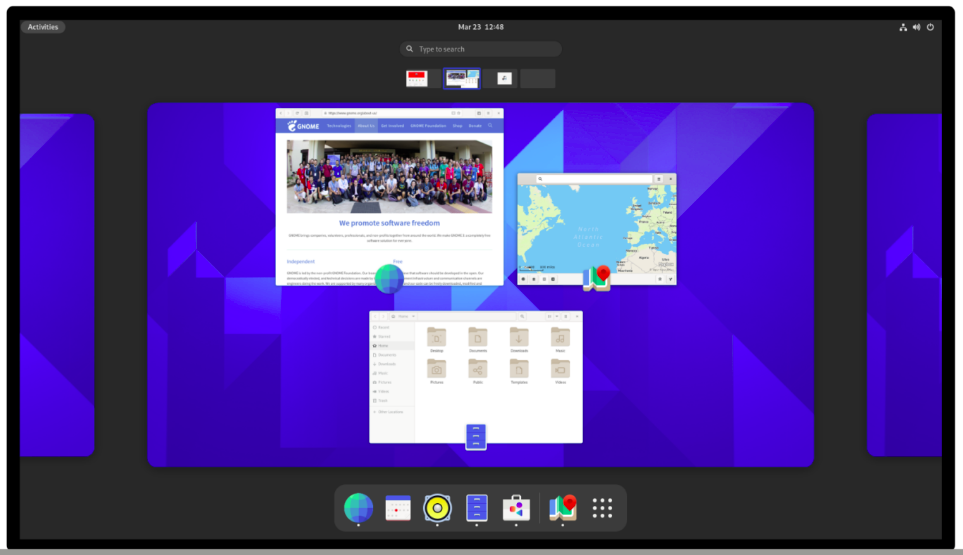
\includegraphics[width=250pt]{chapters/part-1/figures/gnome_demo.png}
	\caption{GNOME desktop environment.} \label{ch:bitl:fig:gnomedemo}
\end{figure}

\begin{figure}[htbp]
	\centering
	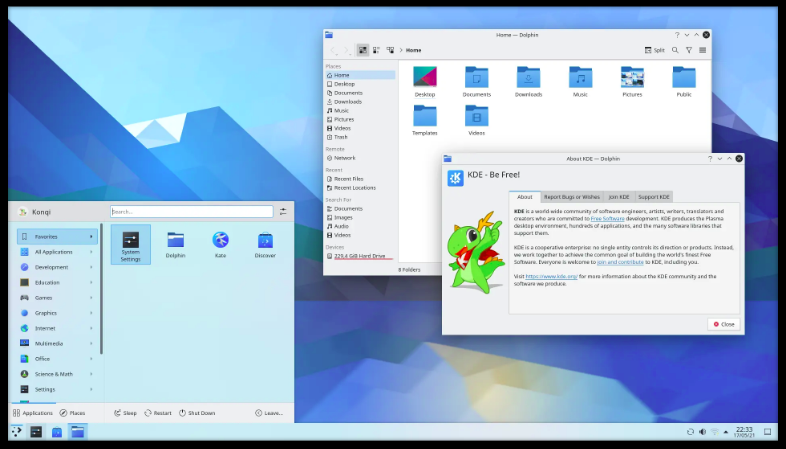
\includegraphics[width=250pt]{chapters/part-1/figures/kde_demo.png}
	\caption{KDE desktop environment.} \label{ch:bitl:fig:kdedemo}
\end{figure}

\begin{figure}[htbp]
	\centering
	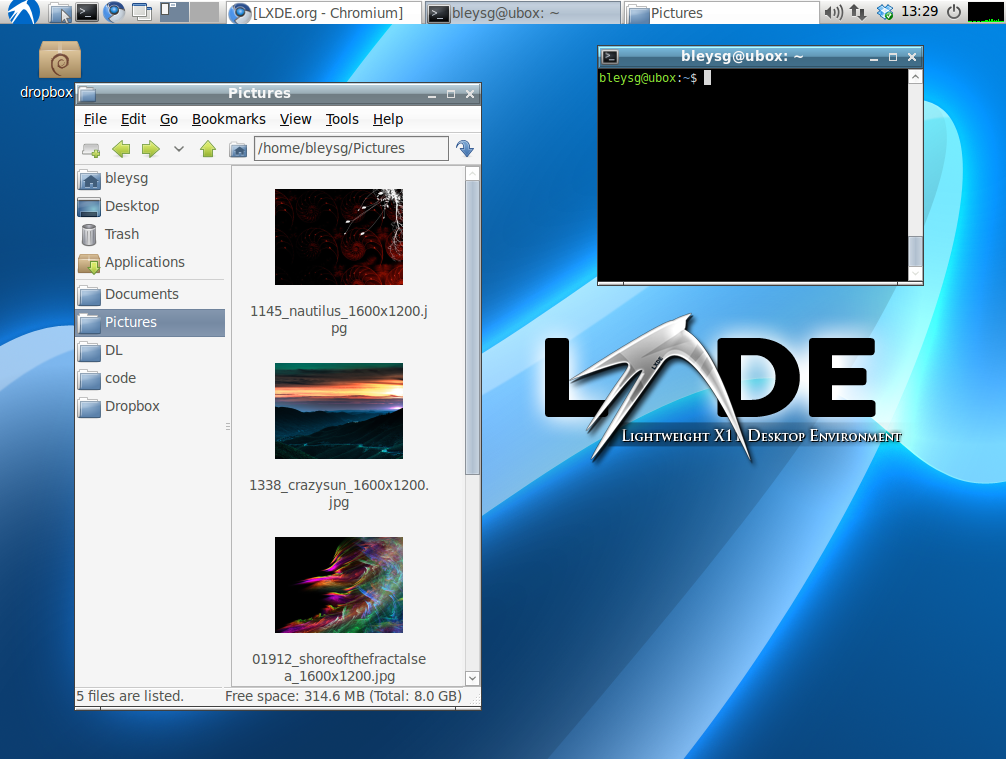
\includegraphics[width=250pt]{chapters/part-1/figures/lxde_demo.png}
	\caption{LXDE desktop environment.} \label{ch:bitl:fig:lxdedemo}
\end{figure}

\begin{figure}[htbp]
	\centering
	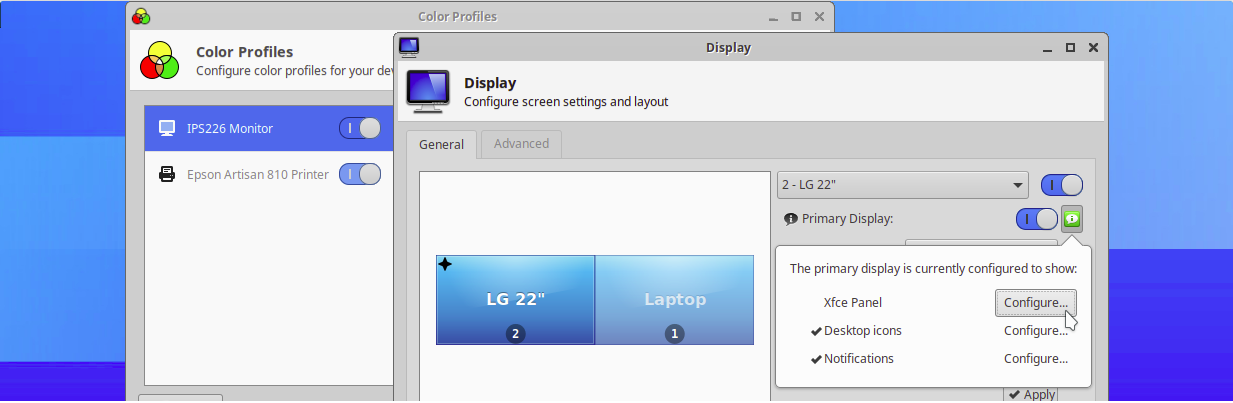
\includegraphics[width=250pt]{chapters/part-1/figures/xfce_demo.png}
	\caption{Xfce desktop environment.} \label{ch:bitl:fig:xfcedemo}
\end{figure}

It is possible to install multiple desktop environments on one machine, in which case the user can choose which desktop environment to use each time the computer is started.

\section{Linux Installation}

Linux can be installed both on a fixed hard drive or on a mobile storage such as a thumb drive. The installation of different distributions may differ. Thanks to the graphical installation tools for the popular distributions, the installations can be done fairly easily.

Instructions of installing Ubuntu is given by \textit{https://ubuntu.com}. Instructions of installing Fedora is given by \textit{https://getfedora.org}. For the use of RHEL, consult with Red Hat at \textit{https://www.redhat.com}. Red Hat provides different types of RHEL licenses for different using purpose, including developer license, which is cheaper than a standard enterprise-level license and serves well for learning purpose.

\chapter{Shell} \label{ch:sb}

Linux command line interface (CLI), usually known as the ``shell'' (also known as ``terminal''), is the most available, flexible and powerful tool for the users and programs to interact with the OS and perform certain actions.

Notice that the use of the shell is not compulsory for casual users when the graphical desktop is present. Still, it is strongly recommended that the users shall understand at least the basics of the shell since it is more flexible and powerful than the graphical desktop and hence can become handy time to time when configuring certain software.

Linux shell will be used rapidly in the remaining of this notebook.

\section{Shell as a Command Line Interface}

Linux's default CLI, usually known as the ``shell'', was invented before the graphical tools, and it has been more powerful and flexible than the graphical tools from the first day. On those machines where no graphical desktops are installed, the use of shell is critical.

\subsection{Shell Types}

There are different types of shells for Linux. The most commonly used shell is the ``bash shell'' which stands for ``Bourne Again Shell'', derived from the ``Bourne Shell'' used in UNIX. Unless otherwise mentioned, the shell we refer to in the remaining of the notebook is bash shell. An example of a shell that calculates Fibonacci series is given below. Notice that in practice shell is mainly used for interaction with the OS and not for software development, data processing or numerical calculation. The example is only for demonstration.

\begin{lstlisting}
#!/usr/bin/bash
n=10
function fib
{
  x=1; y=1
  i=2
  echo "$x"
  echo "$y"
  while [ $i -lt $n ]
  do
      i=`expr $i + 1 `
      z=`expr $x + $y `
      echo "$z"
      x=$y
      y=$z
  done
}
r=`fib $n`
echo "$r"
\end{lstlisting}

Some other shells such as ``C Shell'' and ``Korn Shell'' are also popular among certain users or certain Linux distributions. For example, C Shell supports C-like shell programming, which is sometimes more convenient than the shell. In case where the Linux distribution does not have these shells pre-installed, the user can install and use these shells just like installing any other software.

\subsection{Prompt}

With a newly started shell, a string (usually containing username, hostname, current working directory, etc.) followed by either a \verb|$| or \verb|#| should appear. Following the string, the user can key in the shell commands. The string may look different on different machines. An example is given below.
\begin{lstlisting}
<username>@<hostname>:~$
\end{lstlisting}

The above string is called a \textit{prompt}, indicating the start of a user command. By default, for regular users the ending of the prompt is \verb|$|, while for the root user the ending is \verb|#|. The prompt can be customized by changing the environment variable \verb|PS1|. See Sections \ref{ch:sb:subsec:shellenvvar} and \ref{ch:sb:subsec:customizeshell} for details about environment variables and shell customization methods respectively. Commonly used variables in \verb|PS1| are summarized in Table \ref{ch:sb:tab:promptvariable}.

\begin{table}
	\centering \caption{Commonly used variables in prompt.}\label{ch:sb:tab:promptvariable}
	\begin{tabularx}{\textwidth}{lX}
		\hline
		Variable & Description \\ \hline
		\verb|\!| & Command number of the current command in the command history. \\ 
		\verb|\#| & Command number of the current command in the active shell. \\ 
		\verb|\$| & User prompt ``\verb|$|'' for a regular user, or ``\verb|#|'' for the root user. \\
		\verb|\w| & Current working directory entire path. \\ 
		\verb|\W| & Current working directory base name. \\ 
		\verb|\h| & Host name. \\ 
		\verb|\d| & Current date. \\ 
		\verb|\t| & Current time. \\ 
		\verb|\u| & Username. \\ 
		\verb|\s| & Shell name, for example ``\verb|bash|''. \\ 
		\hline
	\end{tabularx}
\end{table}

For the term ``root user'', we are referring to a special user with username and user ID (UID) ``root'' and 0 respectively. This UID gives him the administration privilege over the machine, such as adding/removing users, changing ownership of files, etc. To avoid fatal damage to the entire system by human error, root user shall not be used unless absolutely necessary. For this reason, the root user's authentication is often deactivated by default (by setting its login password to invalid).

Notice that the root user is different from a ``sudoer'', later of which is basically a regular user equipped with \textit{sudo privilege}. A sudoer can temporarily switch to root user by using \verb|sudo su| as follows.
\begin{lstlisting}
<username>@<hostname>:~$ sudo su
[sudo] password for <username>:
root@<hostname>:/home/<username>#
\end{lstlisting}
More about sudo privilege, \verb|sudo| and \verb|su| commands are introduced in Chapter \ref{ch:administration}.

Key in a command and press \verb|Enter| to execute the command. A Linux shell command looks like the following in general
\begin{lstlisting}
$ <command> [<option>] [<input>]
\end{lstlisting}

The shell comes with built-in commands supported by Linux. Different Linux distributions may support different commands. Shell can also trigger the execution of applications installed in the system. More about commonly used commands and applications will be introduced in the remaining of the notebook.

\section{Basic Operations}

Some basic operations of the shell such as setting alias to commands, adding comments, running commands in the background, etc., are introduced here. More are to be covered in the remaining chapters of this notebook.

\subsection{Displaying User/Machine Information}

When login to a new system, the first step is often to check the basic system information, such as hardware configuration, OS version, username, hostname, etc. While there are many ways to do them, each with some features different than others, some handy commands are introduced here.

The following commands show basic information of a user.
\begin{lstlisting}
$ whoami
<username>
$ grep <username> /etc/passwd
<username>:x:<uid>:<gid>:<gecos>:<home-directory>:<shell>
\end{lstlisting}
In the above, \verb|whoami| is used to display the current login user's username. Command \verb|grep| is used to search content from files or folders, in this case the user name from \verb|/etc/passwd| file which stores user information. This should return the username, the password (for encrypted password, an ``x'' is returned), UID, group id (GID), user id info (GECOS), home directory and default shell location of the user.
Another command \verb|id| also returns the UID and GID information of the current user. More about commands such as \verb|grep| will be introduced in later chapters.

The following commands show the date and hostname of the machine.
\begin{lstlisting}
$ date
<date, time and timezone>
$ hostname
<hostname>
\end{lstlisting}

The following command \verb|lshw| lists down hardware information in details. Sudo privilege is recommended when using this command, to give more detailed and accurate information of the system. Sometimes the displayed information can be too detailed. Use \verb|-short| argument with the command to shorten the output.
\begin{lstlisting}
$ sudo lshw
\end{lstlisting}

\subsection{Set Alias and Shortcuts}

Command \verb|alias| is used to create short-cut keys for commands and associated options, which makes it more convenient for the system operators to work on the shell. Some alias has already been created automatically when the shell is started. Use \verb|alias| to check the existing alias in the shell. An example is given below.

\begin{lstlisting}
$ alias
alias egrep='egrep --color=auto'
alias fgrep='fgrep --color=auto'
alias grep='grep --color=auto'
alias l='ls -CF'
alias la='ls -A'
alias ll='ls -alF'
alias ls='ls --color=auto'
\end{lstlisting}

A temporary alias can be added to the shell by using
\begin{lstlisting}
$ alias <shortcut command>='<original command and options>'
\end{lstlisting}
for example
\begin{lstlisting}
$ alias pwd='pwd; ls -CF'
\end{lstlisting}

To permanently add alias to the shell, the alias needs to be added to the shell start scripts such as \verb|~/.bashrc|.

\subsection{Check Manuals of a Command}

Many commands can be used flexibly and it is impossible to illustrate all their details. Consider use the following two methods to check the detailed manual about a command.
\begin{lstlisting}
$ man <command>
$ <command> --help
\end{lstlisting}

\subsection{Use Comments}

Use \verb|#| to lead a single-line comment. For multi-line comment, use \verb|:' ... '|. Examples are given below.
\begin{lstlisting}
# this is a single-line comment
:'
this is a multi-line comment
this is a multi-line comment
this is a multi-line comment
'
\end{lstlisting}

\subsection{Others}

Use \verb|history| to check history commands. Use \verb|!<history command index>| to repeat a history command, or use \verb|!!| to repeat the latest previous command. It is possible to disable history recording function for privacy purpose.

Use \verb|&| after a command to run it in the background.

Use \verb|;| to write two commands in a single row, and execute them sequentially with one click of \verb|Enter|.

Use \verb|\| to break a single-line command into multiple rows when the command is very long.

\section{Shell Environment Variables}\label{ch:sb:subsec:shellenvvar}

To execute a command by its name, the OS needs to know where the command is located at. Commonly used commands shall be included in the PATH environment of the shell, so that they can be executed anytime from any working directory. The PATH environment is a collection of directories in the system, and it is initialized automatically when the shell is started. Check the PATH environment by
\begin{lstlisting}
$ echo $PATH
<directory-1>:<directory-2>:<directory-3>: ...
\end{lstlisting}
where \verb|echo| displays a line of text, and \verb|$PATH| is a built-in environment variable that records the PATH environment of the current shell. 

The default PATH environment often contains the following directories. 
\begin{itemize}
\item \verb|/bin|, \verb|/usr/bin|: commonly used Linux built-in commands
\item \verb|/sbin|, \verb|/usr/sbin|: commonly used Linux built-in commands for administrators
\item \verb|/home/<username>/bin|: commands defined by a user
\end{itemize}
To determine the location of a particular command, use \verb|type| if the command can be found in the PATH environment. Alternatively, use \verb|locate|, \verb|mlocate| to search all the accessible files in the system to find a command. The syntax is demonstrated below.
\begin{lstlisting}
$ type <command>
<command-location>
\end{lstlisting}

In addition to \verb|PATH|, there are other shell environment variables for the user to monitor and control the OS. Table \ref{ch:sb:tab:shellenvironmentvars} summarizes commonly used shell environment variables. Command \verb|echo $<variable-name>| can be used to check the values of these variables. Use command \verb|env| to check a list of environment variables in the shell.

\begin{table}
	\centering \caption{Commonly used shell environment variables.}\label{ch:sb:tab:shellenvironmentvars}
	\begin{tabularx}{\textwidth}{lX}
		\hline
		Variable & Description \\ \hline
		\verb|BASH| & Full pathname of the \verb|bash| command. \\ 
		\verb|BASH_VERSION| & Current version of the \verb|bash| command. \\ 
		\verb|EUID| & Effective user ID number of the current user, which is assigned when the shell starts, based on the user's entry in \verb|/etc/passwd|. \\ 
		\verb|HISTFILE| & Location of the history file. \\ 
		\verb|HISTFILESIZE| & Maximum number of history entries. \\ 
		\verb|HISTCMD| & The number index of the current command. \\ 
		\verb|HOME| & Home directory of the current user. \\ 
		\verb|PATH| & Path to available commands. \\ 
		\verb|PWD| & Current directory. \\ 
		\verb|OLDPWD| & Previous directory. \\ 
		\verb|SECONDS| & Number of seconds since the shell starts. \\ 
		\verb|RANDOM| & Generating a random number between 0 and 99999. \\
		\hline
	\end{tabularx}
\end{table}

The environmental variables can be created or updated as follows.
\begin{lstlisting}
<variable-name> = <variable-value> ; export <variable-name>
\end{lstlisting}
For example,
\begin{lstlisting}
PATH = $PATH:/getstuff/bin ; export PATH
\end{lstlisting}
adds a new directory \verb|/getstuff/bin| to the \verb|PATH| environmental variable. This allows temporary change to the PATH environment variable. Notice that each time the shell is restarted, the environmental variables are also reset. 

To permanently change the value of an environmental variable, consider customizing the shell. Shell customization is introduced in Section \ref{ch:sb:subsec:customizeshell}.

\section{Customization of Shell} \label{ch:sb:subsec:customizeshell}

Shell configuration files are loaded each time a new shell starts. User-defined permanent configurations (such as useful alias) can be put into these files so that the configurations can be implemented automatically. Some useful files are summarized in Table \ref{ch:sb:tab:shellconfig}.

\begin{table}
	\centering \caption{Shell configuration files.}\label{ch:sb:tab:shellconfig}
	\begin{tabularx}{\textwidth}{lX}
		\hline
		File pathname & Description \\ \hline
		\verb|/etc/profile| & The environment information for every user, which executes upon any user logs in. Root privilege is required to edit this file.  \\ 
		\verb|/etc/bashrc| & Bash configuration for every user, which executes upon any user starts a shell. Root privilege is required to edit this file. \\ 
		\verb|~/.bash_profile| & The environment information for current user, which executes upon the user logs in. \\ 
		\verb|~/.bashrc| & Bash configuration for current user, which executes upon the user starts a shell. \\ 
		\verb|~/.bash_logout| & Bash log out configuration for current user, which executes upon the user logs out or exit the last bash shell. \\ \hline
	\end{tabularx}
\end{table}

To customize the shell behavior for a user, the most commonly method is to edit his \verb|~/.bashrc| which is executed automatically each time he starts a shell.

\section{Shell Script Programming Basics}

A truly power feature of the shell is its ability to redirect inputs/outputs of commands, thus to chain the commands together. Meta-characters pipe (\verb?|?), ampersand (\verb|&|), semicolon (\verb|;|), dollar (\verb|$|), parenthesis (\verb|()|), square bracket (\verb|[]|), less than sign (\verb|<|), greater than sign (\verb|>|), double greater than sign (\verb|>>|), error greater than sign (\verb|2>|) and a few more more, are used for this feature. Details are given below.

The pipe (\verb$|$) connects the output of the first command to the input of the second command. The following example searches keyword ``function'' in \verb|calculate_fib.sh| which was given previously.
\begin{lstlisting}
$ cat calculate_fib.sh | grep function
function fib
\end{lstlisting}
where \verb|cat| concatenates files and print on the standard output, and \verb|grep| prints lines that match patterns in each file.

The semicolon (\verb|;|) allows inputting multiple commands in the same line in the script. The commands are then executed one after another from left to right.

The ampersand (\verb|&|) can be put in the end of a line so that the command on that line will run in the background. The commands or process running in the background does not occupy the shell standard display, and the users can continue working on other commands in parallel. This is particularly useful when a task is going to take a long time to be executed. To manage the tasks running in the background, check more details in Chapter \ref{ch:pm}.

Use the dollar sign \verb|$| (not the prompt) to indicate a command expansion. The command in \verb|$(<command>)| will be executed as a whole, then treated as a single argument. The content in \verb|()| is sometimes called sub-shell. For example, to display the function defined in \verb|calculate_fib.sh| previously,
\begin{lstlisting}
$ echo Display functions: $(cat calculate_fib.sh | grep function)
Display functions: function fib
\end{lstlisting}
Below is another example to count the number of files/folders in the current directory.
\begin{lstlisting}
$ echo There are $(ls -a | wc -w) files in this directory.
There are 69 files in this directory.
\end{lstlisting}
where \verb|wc| counts the number of lines, words or bytes in a file.

Use \verb|$[<arithmetic expression>]| for simple calculations, such as
\begin{lstlisting}
$ echo 1+1=$[1+1]
1+1=2
\end{lstlisting}

The dollar sign \verb|$| is also used to expand the value of a variable, either environmental variable or self-defined variable, as explained previously in \ref{ch:sb:subsec:shellenvvar}. An example is \verb|$PATH| which returns the PATH environment.

The less than sign \verb|<| and greater than sign \verb|>| are used to map the input/output of a command to a file instead of the standard input and output. An example using command \verb|sort| together with input direction \verb|<| is given as follows. Considering sorting characters ``a'', ``c'', ``b'', ``g'', ``e'', ``f'', ``d'' using \verb|sort| command. The letters are input from the console as follows. Use \verb|ctrl+D| to quit the input, and the output after sorting will be displayed in the console as follows.
\begin{lstlisting}
$ sort
a
c
b
g
e
f
d
a
b
c
d
e
f
g
\end{lstlisting}
For demonstration purpose, create a file \verb|before_sort| in the current working directory. Inside \verb|before_sort| are letters ``a'', ``c'', ``b'', ``g'', ``e'', ``f'', ``d'', each occupying a separate row. There are several ways to prepare the file which will be explained shortly. For now, just assume that the file already exists. Use \verb|cat| to quickly check its content as follows.
\begin{lstlisting}
$ cat before_sort
a
c
b
g
e
f
d
\end{lstlisting}

Use \verb|sort| to sort \verb|before_sort| as follows. In this case, the input to \verb|sort| becomes a file, rather than the standard input from the keyboard. Notice that in this example, \verb|sort before_sort| also works, as \verb|sort| will by default take its first argument as the location of the file to be sorted.
\begin{lstlisting}
$ sort < before_sort
a
b
c
d
e
f
g
\end{lstlisting}

Use \verb|>| to redirect the output of a command to a file as given in the following example.
\begin{lstlisting}
$ sort < before_sort > after_sort
$ cat after_sort
a
b
c
d
e
f
g
\end{lstlisting}
where \verb|sort| does not output the result to the console, but instead saves the result in a file named \verb|after_sort|. The double greater sign \verb|>>| works similarly with \verb|>| except that \verb|>>| will append the output to an existing file, while \verb|>| overwrites the existing file.

With the above been said, it is possible to use the following to create the \verb|before_sort| file that has been used in the example.
\begin{lstlisting}
$ echo -e "a\nc\nb\ng\ne\nf\nd\n" > before_sort
\end{lstlisting}

The error greater sign \verb|2>|, \verb|2>>| works similarly with \verb|>|, \verb|>>| except that instead of redirecting standard output messages, it redirects the error messages.





%\chapterauthor{Author Name}{Author Affiliation}
%\chapterauthor{Second Author}{Second Author Affiliation}
\chapter{Text File Editing} \label{ch:tfe}

Many text editors are supported in Linux, to name a few, Vim, Emacs, gedit, Visual Studio Code. These text editors come with different features. Some of the text editors even provide \myabb{Integrated Development Environment}{IDE} features.

Among the vast number of choices, Vim is probably the most popular one. It works perfectly in a shell environment without relying on graphical desktop, thus is adopted by many Linux distributions as the built-in text editor. Vim is introduced in this chapter, followed by a brief review of some other commonly used text editors.

\section{General Introduction to Vim}

\mync{Vi IMproved}[Vim] is a free and open-source software developed by Bram Moolenaar et al. It is an expansion to the \mync{Vi} text editor to include features such as syntax highlighting, etc., and has become the default text editor of many Unix/Linux based operating systems.

Some people claim Vim to be the most powerful text file editor and IDE for programming on a Linux machine (and potentially on all computers and servers). The main reasons are as follows.
\begin{itemize}
  \item Vim is usually built-in to Linux during the operating system installation, making it the most available and cost-effective text editor.
  \item Vim can work on machines where graphical desktop is not supported.
  \item Vim is light in size and is suitable to run even on an embedded system.
  \item Vim operations are done mostly via mode switch and shortcut keys; as a result, \textbf{the brain does not need to halt and wait for the hand to grab and move the mouse}, thus speeding up the text editing.
  \item Vim is highly flexible and can be customized according to the user's habit (for example, through \verb|~/.vimrc|), and it allows the users to define shortcut keys.
  \item Vim can automate repetitive operations by defining macros.
  \item Vim can be integrated with third-party tools which boost its features to a higher level.
\end{itemize}

Vim can become very powerful and convenient for the user if he is very used to it. However, Vim is not as intuitive as other text editors such as gedit, and there might be a learning curve for the beginners.

Bram Moolenaar, the original inventor of Vim, passed away on August 3, 2023 at the age of 62. His project Vim has been taken over by the contributors from community. 

\section{Vim Modes} \label{ch:tfe:subsec:vimgeneralintro}

Unlike other text editors, Vim defines different ``modes'' during the operation, each mode has some unique features. For example, in the \textbf{insert} mode, Vim maps keyboard inputs with the text file just like an conventional text editor. In the \textbf{normal} mode (this is the default mode when opening Vim), Vim uses useful and customizable shortcut keys to quickly navigate the document and perform operations such as cut, copy, paste, replace, search, and macro functions. In the \textbf{virtual} mode, Vim allows the user to select a block of content for further editing. In the \textbf{cmdline} mode, Vim takes order from command lines and interact with Linux to perform tasks such as save and quit.

The following Table \ref{ch:tfe:tab:vimmodes} summarizes the commonly used modes in Vim.
\begin{table}
  \centering \caption{Commonly used modes in Vim.}\label{ch:tfe:tab:vimmodes}
  \begin{tabularx}{\textwidth}{lX}
    \hline
    Mode & Description \\ \hline
    Normal & Default mode. It is used to navigate the cursor in the text, search and replace text pieces, and run basic text operations such as undo, redo, cut (delete), copy and paste. \\ 
    Insert & It is used to insert keyboard inputs into the text, just like commonly used text editors today. \\ 
    Visual & It is similar to normal mode but areas of text can be highlighted. Normal mode commands can be used on the highlighted text. \\ 
    Cmdline & It takes in a single line command input and perform actions accordingly, such as save and quit. \\
    \hline
  \end{tabularx}
\end{table}

As a start, the following basic commands can be used to quickly create, edit and save a text file using vim. In home directory, start a shell and key in
\begin{lstlisting}
$ vim testvim
\end{lstlisting}
to create a file named ``testvim'' and open the file using Vim. Notice that in some Linux versions, Vi might be aliased to Vim by default.

In the opened file, use \verb|Esc| and \verb|i|/\verb|a| (insert/append) to switch between normal mode and insert mode. Notice that in the normal mode, the cursor is on a character. When using the insert command, the insertion cursor is put to the left of that character, whereas when using the append command, the insertion cursor is put to the right of that character. 

In the normal mode, use \verb|h|, \verb|j|, \verb|k|, \verb|l| to navigate the position of the cursor. 

Finally, in the normal mode, use \verb|:w| to save the file, and \verb|:q| to quit Vim, or use \verb|:wq| to save and quit Vim.

The above basic commands and their relationships are summarized in Fig.~\ref{ch:tfe:fig:vimbasicmodeswitching}. A flowchart to create/open, edit, save, and quit a text file using the aforementioned commands are given in Fig.~\ref{ch:tfe:fig:vimbasicoperationflowchart}.

\begin{figure}[htbp]
\centering
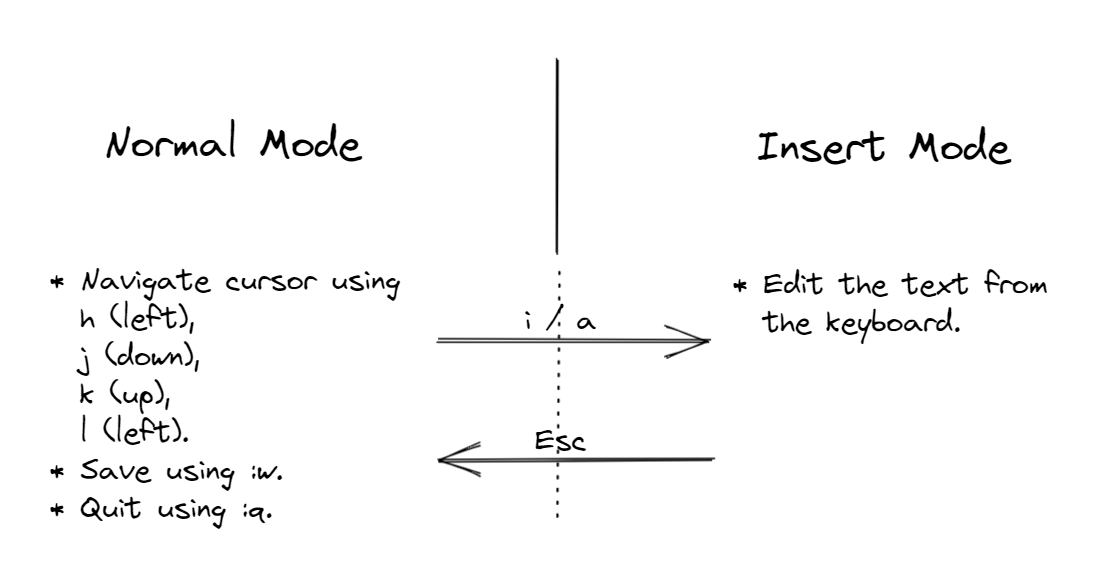
\includegraphics[width=250pt]{chapters/part-1/figures/vimbasicmodeswitching.png}
\caption{Mode switching between normal mode and insert mode, and basic functions associated with the modes.} \label{ch:tfe:fig:vimbasicmodeswitching}
\end{figure}

\begin{figure}[htbp]
\centering
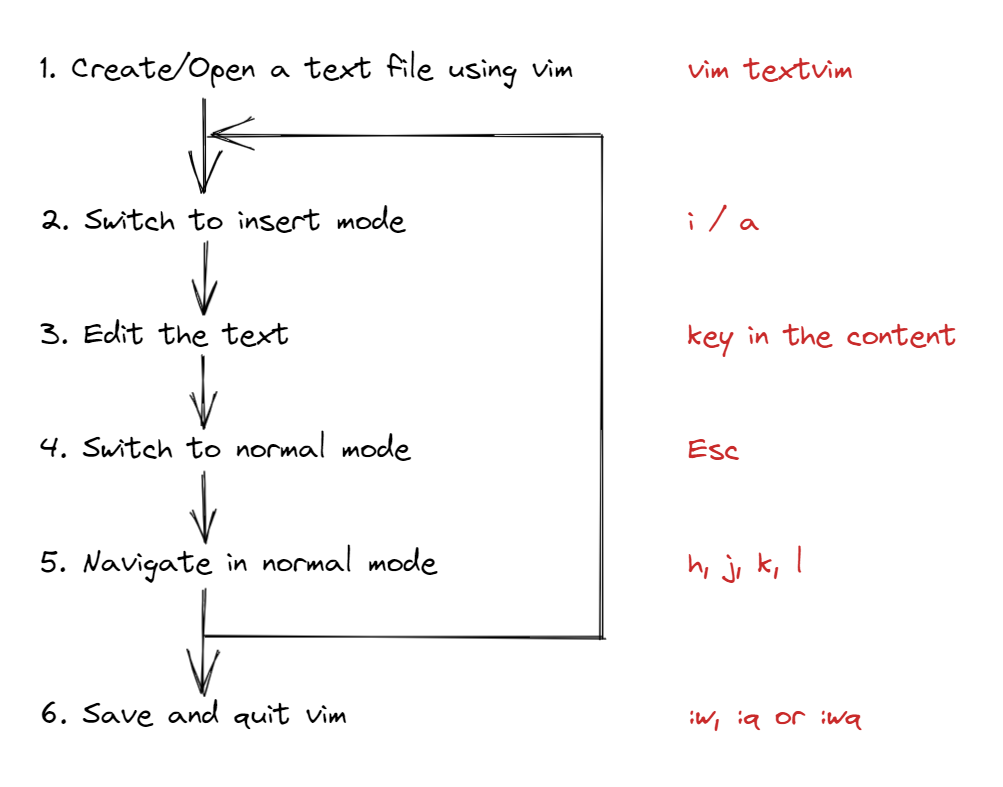
\includegraphics[width=250pt]{chapters/part-1/figures/vimbasicoperationflowchart.png}
\caption{A flowchart for simple creating, editing and saving of a text file using Vim.} \label{ch:tfe:fig:vimbasicoperationflowchart}
\end{figure}

There are other shortcuts to switch from normal mode to insert mode. Some of them are summarized in Table \ref{ch:tfe:tab:switchtoinsert}.

\begin{table}
  \centering \caption{Commonly used shortcuts to switch from normal mode to insert mode.}\label{ch:tfe:tab:switchtoinsert}
  \begin{tabularx}{\textwidth}{lX}
    \hline
    Operator & Description \\ \hline
    \verb|i| & Insert before the character at the cursor. \\ 
    \verb|I| & Insert at the beginning of the row at the cursor. \\ 
    \verb|a| & Insert after the character at the cursor. \\ 
    \verb|A| & Insert at the end of the row at the cursor. \\ 
    \verb|o| & Create a new row below the cursor and switch to insert mode. \\ 
    \verb|O| & Create a new row above the cursor and switch to insert mode. \\
    \hline
  \end{tabularx}
\end{table}

\section{Vim Profile Configuration}

With the basic operations introduced in Section \ref{ch:tfe:subsec:vimgeneralintro}, we are able to create and edit a text file as we want to, just like using any other text editor. Though at this point the advantages of using Vim over other text editors are not obvious yet, the Vim editor is at least useable.

Before introducing more advanced features of Vim, for better user experience we can now customize the user profile to suit our individual habit. Notice that the customization is completely optional and personal. This section only introduces the idea and basic methods such as re-mapping keys and creating user-defined shortcuts. Everything introduced here are merely examples and it is completely up to the user how to design and implement his own profile.

In Linux, navigate to home directory. Create the following path and file \verb|~/.vim/vimrc| or \verb|~/.vimrc|. Open the \verb|vimrc| file as a blank file using Vim. The individual user profile can be customized here.

There are many readily available \verb|vimrc| profiles shared in the community. Feel free to use them as a reference when creating a new profile.

\subsection{Mapping Shortcuts}

It is desirable to re-map some keys to speed up the text editing. For example, by mapping \verb|jj| to \verb|Esc| in insert mode, one can switch from insert mode to normal mode more quickly (notice that consequent ``jj'' is rarely used in English). Another example coud be mapping \verb|j|, \verb|k|, \verb|i| to \verb|h|, \verb|j|, \verb|k| respectively in normal and visual modes, making the navigation more intuitive. In that case, another key needs to be mapped to \verb|i| because insert command is very useful and we do not want to lose it.

The mapping of keys and keys combinations can be done as follows in \verb|vimrc|.
\begin{lstlisting}
inoremap jj <Esc>
noremap j h
noremap k j
noremap i k
noremap h i
\end{lstlisting}
where \verb|inoremap| is used to map keys (combinations) in insert mode, and \verb|noremap| in normal and visual modes.

The upper case letter \verb|S| and lower case letter \verb|s| in normal mode are originally used to delete and substitute texts, and they are rarely used due to the more powerful shortcut \verb|c| which does similar tasks. We can re-map \verb|S| to saving, and disable \verb|s|. Similarly, upper case letter \verb|Q| is mapped to quitting Vim.
\begin{lstlisting}
noremap s <nop>
map S :w<CR>
map Q :q<CR>
\end{lstlisting}
where \verb|<nop>| stands for ``no operation'' and \verb|CR| stands for the ``enter'' key on the keyboard. The keyword \verb|map| differs from \verb|noremap| in the sense that \verb|map| is for recursive mapping.

\subsection{Syntax and Color Scheme}

By default Vim displays white colored contents on a black background. Use the following command in \verb|vimrc| to enable syntax highlighting or change color schemes. Use \verb|:colorscheme| in cmdline mode in Vim to check for available color schemes.
\begin{lstlisting}
syntax on
colorscheme default
\end{lstlisting}

The following setups in \verb|vimrc| displays the row index and cursor line (a underline at cursor position) of the text, which can become handy during the programming. Furthermore, it sets auto-wrap of text when a single row is longer than the displaying screen.
\begin{lstlisting}
set number
set cursorline
set wrap
\end{lstlisting}

The following command opens a ``menu'' when using cmdline mode, making it easier to key in commands.
\begin{lstlisting}
set wildmenu
\end{lstlisting}

\subsection{Other Useful Setups}

Use \verb|scrolloff| to make sure that when scrolling in Vim, there are always margins lines in the top and bottom of the screen, so that the cursor is always close to the centre of the screen.
\begin{lstlisting}
set scrolloff=3
\end{lstlisting}

Enable spell check in Vim as follows.
\begin{lstlisting}
map sc :set spell!<CR>
\end{lstlisting}
where \verb|sc| can be used to quickly turn on and off the spell check function. In addition, when the cursor is put on the wrongly spelled word, use \verb|z=| to open a list of possible corrections.

\subsection{Plug Tools}

In the Linux community, many plug tools have been created to add useful features for Vim. As a demonstration, in this section \textit{vim-plug}, a light-size vim plugin management tool created on GitHub, is used to install selected Vim plugins. Details about \textit{vim-plug} can be found at GitHub under \textit{junegunn/vim-plug}.

Following the instructions given by GitHub under \textit{junegunn/vim-plug}, to use \textit{vim-plug} on Linux, the very first step is to use \textit{cURL}, a command-line tool for transferring data specified with URL syntax, to download \textit{vim-plug}. To install \textit{cURL} if it has not been installed, use
\begin{lstlisting}
$ sudo yum install curl # red-hat-based distributions
$ sudo apt install curl # debian-based distributions
\end{lstlisting}

With \textit{cURL} installed, use the following in the shell to install \textit{vim-plug}
\begin{lstlisting}
$ curl -fLo ~/.vim/autoload/plug.vim --create-dirs \
    https://raw.githubusercontent.com/junegunn/vim-plug/master/plug.vim
\end{lstlisting}
In the very beginning of \verb|vimrc|, add the following to specify the plugins to be installed. As an example, \textit{vim-airline/vim-airline} and \textit{joshdick/onedark.vim} are to be installed, the first of which adds a status line at the bottom of the Vim window, and the second adds a popular color scheme ``onedark''.
\begin{lstlisting}
call plug#begin()
Plug 'vim-airline/vim-airline'
Plug 'joshdick/onedark.vim'
call plug#end()
\end{lstlisting}
Finally, reload \verb|vimrc|, then run \verb|:PlugInstall| in cmdline mode to install the plugins. Use \verb|colorscheme onedark| instead of \verb|colorscheme default| in \verb|vimrc| to enjoy the onedark color scheme.

Notice that instead of setting up configurations permanently in \verb|vimrc|, the user can also apply a setup in cmdline mode for temporary use in an open session. A full list of \verb|vimrc| configurations used in this chapter can be found in the appendix.

\section{Basic Operations in Vim}

In normal mode, the most frequently used operation is probably \verb|u| for undo. Other commonly used operations, such as delete, cut, copy, paste, replace and search, are mostly done in normal mode through shortcut keys. For example, \verb|dd| deletes (cuts) the entire row at the cursor and \verb|p| pastes the content in the clipboard to the cursor position. For beginners, remembering shortcut keys can be difficult. Therefore, it is suggested looking for the consistent patterns of the different commands, rather than brute-force remembering all the operations.

Many Vim shortcut keys in normal mode has the following pattern: an operator command directly followed by a motion command without space in between.
\begin{lstlisting}
<operator><motion>
\end{lstlisting}
The operator command tells Vim what to do (say, copy), and the motion command tells the applicable range of the operation (say, a row, or a word, or a character). Some operator commands may work alone without motion commands.

\subsection{Cut, Change, Copy and Paste}

The following lines taken from Wikipedia under ``William Shakespeare'' is used as an example to demonstrate delete/cut, change, copy and paste functions. In the text file, each sentence takes a separate row as shown in Figure \ref{ch:tfe:fig:vimdemo1}.

\begin{shortbox}
William Shakespeare (bapt. 26 April 1564 – 23 April 1616) was an English playwright, poet and actor, widely regarded as the greatest writer in the English language and the world's greatest dramatist.

He is often called England's national poet and the ``Bard of Avon'' (or simply ``the Bard'').
\end{shortbox}

\begin{figure}[htbp]
\centering
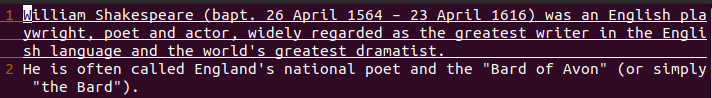
\includegraphics[width=250pt]{chapters/part-1/figures/vimdemo1.png}
\caption{A piece of text of ``William Shakespeare'', for demonstration.} \label{ch:tfe:fig:vimdemo1}
\end{figure}

Use either \verb|x| or \verb|X| to delete the character at the cursor or previous to the cursor, respectively. To delete multiple characters, one way is to press \verb|x| or \verb|X| multiple times (or hold the keys). Alternatively, it is possible for Vim to automatically repeat the procedure. For example, \verb|20x| tells Vim to perform \verb|x| for 20 times. The same applies for other operators or motions commands. For example, \verb|10l| executes \verb|l| for 10 times, moving the cursor to the right for 10 characters.

Operator \verb|d|, similar with \verb|dd|, deletes the contents of the text, but it requires a motion command and can be used more flexibly. The motion shall tell Vim the applicable range to delete/cut.

For example, \verb|dl| deletes one character to the right, i.e. deletes the character at the cursor just like \verb|x|. Likewise, \verb|dh| deletes one character to the left just like \verb|X|. Similarly, \verb|d20l| deletes 20 characters to the right, where ``20l'' as a whole plays as the motion of ``20 characters to the right''. A combination by using things like \verb|5d4l| also works and leads to the same result as $20=5\times 4$.

Command \verb|d| can be used even more flexibly. For example, by using word-related motions, \verb|d| can delete/cut by words instead of by characters. Move the cursor to the beginning of a word, (for example, ``S'' in ``Shakespeare''), use \verb|dw| to delete the word. The word motion \verb|w| is similar with \verb|l|, except that \verb|l| directs to the next character, while \verb|w| directs to the beginning of next word. Similarly, \verb|b| directs to the beginning of the current/previous word. Thus, \verb|db| can be used to delete word to the left. Examples \verb|d10b|, \verb|10db|, \verb|d20w|, \verb|5d4w| can be used to delete multiple words at a time. Motions \verb|w| and \verb|b| can also be used to navigate in the text just like \verb|l| and \verb|h|.

When in the middle of a word, \verb|dw| will delete the characters from the cursor to the beginning character of the next word. For example, if the cursor is currently at ``k'' in ``Shakespeare'', \verb|dw| will delete ``kespeare '' (notice that the space between ``Shakespeare'' and ``(bapt.'' will also be deleted). To delete from the beginning of the word instead, you can use \verb|b| first to navigate back to the beginning of the word, then apply \verb|dw|. Alternatively, use ``inner-word'' motion \verb|iw| to indicate that the whole word of the cursor shall be deleted, i.e., \verb|diw| to delete ``Shakespeare''. The space after ``Shakespeare'' will stay. To remove that space together with the word ``Shakespeare'', use \verb|daw| instead. More about motions \verb|aw| will be introduced shortly.

In addition to character-related motions \verb|h|, \verb|l| and word-related motions  \verb|b|, \verb|w|, there are similar motions for sentence \verb|(| (previous), \verb|)| (next) and paragraph \verb|{| (previous), \verb|}| (next). There are also inner-sentence motion \verb|is|, inner-paragraph motion \verb|ip|, inner-quotation motion \verb|i'|, \verb|i"|, \verb|i`| and inner-block motion \verb|i(|, \verb|i<|, \verb|i{|, and many more. For example, when the cursor is at ``A'' of ``26 April 1564'', \verb|di(| will delete everything inside ``()'', i.e. deleting ``bapt. 26 April 1564 - 23 April 1616''.

The operators and motions introduced so far are summarized in Tables \ref{ch:tfe:tab:deletecut} and \ref{ch:tfe:tab:motion}. Notice that motions \verb|aw|, \verb|as|, \verb|ap| are also given in the table. They are similar with their corresponding \verb|iw|, \verb|is|, \verb|ip| except that when deleting, the sequential blank space (for word and sentence) or blank row (for paragraph) will also be deleted.

\begin{table}
  \centering \caption{Commonly used operators related to delete/cut, change, copy and paste.}\label{ch:tfe:tab:deletecut}
  \begin{tabularx}{\textwidth}{lX}
    \hline
    Operator & Description \\ \hline
    \verb|x| & Delete/Cut the character at cursor. \\ 
    \verb|X| & Delete/Cut the character before cursor. \\ 
    \verb|dd| & Delete/Cut the entire row. \\ 
    \verb|d| & Delete/Cut selected text according to the motion command. \\ 
    \verb|cc| & Change the entire row. \\ 
    \verb|c| & Change selected text according to the motion command. \\ 
    \verb|yy| & Copy the entire row. \\ 
    \verb|y| & Copy selected text according to the motion command. \\ 
    \verb|p| & Paste clipboard to the cursor. \\
    \hline
  \end{tabularx}
\end{table}

\begin{table}
  \centering \caption{Commonly used motions.}\label{ch:tfe:tab:motion}
  \begin{tabularx}{\textwidth}{lX}
    \hline
    Motion & Description \\ \hline
    \verb|h|, \verb|l| & One character to the left or right. \\ 
    \verb|j|, \verb|k| & One row to the up or down. \\ 
    \verb|b| & First character of the current word, or fist character of the previous word. \\ 
    \verb|e| & Last character of the current word. \\ 
    \verb|w| & First character of the next word. \\ 
    \verb|(|, \verb|)| & One sentence to the previous or next. \\ 
    \lstinline{\{}, \lstinline{\}} & One paragraph to the previous or next. \\ 
    \verb|iw|, \verb|is|, \verb|ip| & Inner-word, inner-sentence, inner-paragraph. \\ 
    \verb|aw|, \verb|as|, \verb|ap| & A word, a sentence, a paragraph (including the end blank). \\ 
    \verb|i'|, \verb|i"|, \verb|i`| & Inner-quotation for different types of quotations. \\ 
    \verb|i(|, \verb|i<|, \verb|i[|, \lstinline{\}} & inner-block for different types of brackets. \\ 
    \verb|0| (zero) & Beginning of the row. \\ 
    \verb|$| & Ending of the row. \\ 
    \verb|gg| & Beginning of the text. \\ 
    \verb|G| & Beginning of the last row of the text. \\
    \hline
  \end{tabularx}
\end{table}

To change contents, use operator \verb|c|, which works the same way as \verb|d| but it automatically switch to insert mode after removing the content. To copy a piece of text to clipboard, use \verb|y| (stands for ``yank'') followed by its associated motion to indicate the range of text. The motions also follow Table \ref{ch:tfe:tab:motion}. To paste the text in the clipboard to the cursor, use \verb|p|. No motion is required.

In addition to Table \ref{ch:tfe:tab:motion}, another commonly used type of motion is to ``find by character''. For example, consider the following row of text. The cursor is currently at letter ``A''.
\begin{lstlisting}
ABCDEFG;HIJKLMN;OPQ;RST;UVW;XYZ
\end{lstlisting}
In normal mode, using \verb|f| followed by a character will navigate the cursor to the nearest corresponding character that appears in the text. For example, \verb|fG| will move the cursor to letter ``G''. Similarly, \verb|f;| will move the cursor to the ``;'' between ``G'' and ``H''. Key in \verb|f;| again and the cursor will move to ``;'' between ``N'' and ``O''. From here key in \verb|2f:| and the cursor will go to ``;'' between ``T'' and ``U'', as it is equivalent to executing \verb|f;| twice. If \verb|df;| is used when the cursor is at letter ``A'', ``ABCDEFG;'' will be deleted.

\subsection{Search in the Text}

In normal mode, use \verb|/<content>| to search a keyword or a phrase. The following customization in \verb|vimrc| shall give a better searching experience.

When searching in the text for a particular word or phrase (searching in the text will be will be covered in a later of the chapter), to make the searching result highlighted, add the following line to the user profile \verb|vimrc|.
\begin{lstlisting}
set hlsearch
exec "nohlsearch"
set incsearch
noremap <Space> :nohlsearch<CR>
set ignorecase
noremap = nzz
noremap - Nzz
\end{lstlisting}
where \verb|hlsearch| enables highlighting all matching results in the text, and \verb|incsearch| enables highlighting texts along with typing the keyword. Vim remembers the keyword from the previous search and may automatically highlight them in the text on a new session. This can be confusing sometimes. To tackle the issue, use command \verb|exec "nohlsearch"| (\verb|exec| in \verb|vimrc| executes a command when starting a new session) after \verb|set hlsearch| to force Vim to clear its searching memory on a new session. Finally, to quit searching, use \verb|:nohlsearch| in cmdline mode and the highlights shall be gone. For convenience, consider mapping it with a customized shortcut key as well, for example to \verb|Space|. As a bonus, set \verb|ignorecase| to ignore case-sensitive during the searching.

Keys \verb|n| and \verb|N| is used to navigate through the searching result, and \verb|zz| is used to pin cursor position in the central of the screen. They are mapped to \verb|-| and \verb|=| in \verb|vimrc|. Notice that they can also be used as motion together with delete/cut, change and copy as given in Table \ref{ch:tfe:tab:deletecut}.

With the above setup, searching for ``he'' using \verb|/he| leads to the following result given in Fig.~\ref{ch:tfe:fig:vimdemo2}.
\begin{figure}[htbp]
\centering
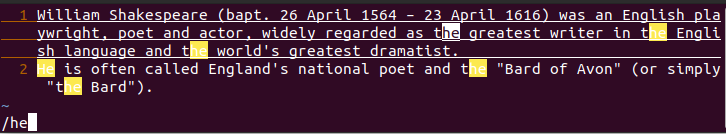
\includegraphics[width=250pt]{chapters/part-1/figures/vimdemo2.png}
\caption{Search ``he'' in the piece of text of ``William Shakespeare''.} \label{ch:tfe:fig:vimdemo2}
\end{figure}
From Fig.~\ref{ch:tfe:fig:vimdemo2}, it can be seen that all appearances of ``he'' (case-insensitive) is highlighted, and the cursor is automatically moved to its first appearance, i.e. ``he'' in ``the greatest writer''. Click \verb|Enter| to enable free move of the cursor.

\subsection{Other Tips}

Use \verb|Ctrl+o|, \verb|Ctrl+i| to ``undo'' and ``redo'' cursor positions, respectively. They only move the cursor position and don't change the actual texts.

To save as a file, use \verb|:w <new path>| in cmdline mode.

In cmdline mode, use \verb|!| to interact with the shell. For example, consider a case where a read-only file needs to be edited and saved by a sudoer who forgot to start Vim using \verb|sudo|. The common \verb|:w| will be rejected. In this case, use \verb|:w !sudo tee %| to perform the save, where \verb|tee| is a Linux command that takes standard input and writes to a file, and \verb|%| stands for the current file. In another example where an existing file's content is to be insert into the current text, navigate the cursor to the place to insert the text, and use \verb|:r !cat <filename>|.

To convert and save the current text into an \textit{html} file, use \verb|:%TOhtml|. From there, the file can be further converted into a PDF file.

\section{Visual Modes}

The use of a mouse makes selecting a block of text very intuitive. In most text editors, the selected text will be highlighted, as if the cursor expands from one character to the entire block of text. Sequentially, operations such as delete and copy can be performed on the selected text.

The three visual modes of Vim, namely ``visual'', ``visual-line'' and ``visual-block'', provide similar experience where the user can select and highlight a block of text.

Use \verb|v| to enter the visual mode, then navigate the cursor to select a block of text. This allows the user to select text between any two characters. An example is given by Fig. \ref{ch:tfe:fig:vimvm1}. Alternatively, use \verb|V| to enter the visual-line mode where multiple lines can be easily selected, and use \verb|<ctrl>+v| to enter visual-block mode to select a rectangular block of text.

\begin{figure}[htbp]
	\centering
	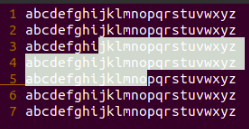
\includegraphics[width=100pt]{chapters/part-1/figures/vimvm1.png}
	\caption{An example of visual mode where a block of text is selected.} \label{ch:tfe:fig:vimvm1}
\end{figure}

In any of the above visual mode, use \verb|:normal + <operation>| to execute operation(s) form the normal mode for each line. This allows convenient editing of multiple lines of text all together. For example, use \verb|V| to select a few lines of contents, followed by \verb|:normal 0iprefix-|. This will insert \verb|prefix-| to all the lines, as if \verb|0iprefix-| is executed in normal mode to all the lines separately. Notice that if \verb|i| has been mapped by another character in normal mode, use that character instead.

Alternatively, in visual-block mode after selecting a block of content, use \verb|I| to enter insert mode and insert content in the first row of the selected block. When existing the insert mode using \verb|<Esc>|, the changes will apply to all selected rows. Similar effect can be achieved.

\section{Vim Macros}

Vim macros is a convenient and power tool for repetitive works. Use \verb|q| in normal mode to start and end a macro recording. The syntax follows
\begin{lstlisting}
q<macro-name><operations>q
\end{lstlisting}
where \verb|<macro-name>| is a single character that labels the macro.

Consider the following example where there is a text file containing the following content
\begin{lstlisting}
apple.jpg
pear.jpg
orange.jpg
banana.jpg
peach.jpg
\end{lstlisting}
and we would like to change the content to
\begin{lstlisting}
image: 'apple.jpg'
ttl: 5
image: 'pear.jpg'
ttl: 5
image: 'orange.jpg'
ttl: 5
image: 'banana.jpg'
ttl: 5
image: 'peach.jpg'
ttl: 5
\end{lstlisting}

In this example, repetitive work is involved and it is time consuming to do it manually if there are thousands of items in the file, and it is better to record a macro to automate the procedure. Navigate the cursor to the first row of the text, and type the following sequence of characters.
\begin{lstlisting}
q<macro name>0iimage: '<Esc>A'<Enter>ttl: 5<Esc>jq
\end{lstlisting}
where \verb|<macro name>| can be any character, for example \verb|s|. The string in the middle \verb|0iimage: '<Esc>A'<Enter>ttl: 5<Esc>j| is the necessary procedure to perform the revision for one row. If everything is done correctly, the file should appear as
\begin{lstlisting}
image: 'apple.jpg'
ttl: 5
pear.jpg
orange.jpg
banana.jpg
peach.jpg
\end{lstlisting}
and the cursor should be at row \verb|pear.jpg|.

To repeat the recorded procedures, use \verb|@<macro-name>|. In this example, just key in \verb|@s| in the normal mode, and the file should appear as
\begin{lstlisting}
image: 'apple.jpg'
ttl: 5
image: 'pear.jpg'
ttl: 5
orange.jpg
banana.jpg
peach.jpg
\end{lstlisting}

Repetitively using \verb|@s| proceeds with the revision. In the case the procedure needs to be repeated for many times, use \verb|<number>@<macro-name>|, in this example \verb|3@s|, to complete the remaining task.

\section{File Explorer and Screen Splitting}

Many IDEs come with project folder navigation and screen splitting features. In these IDEs, there is often a built-in file explorer, from where the user can navigate in the file system, select a file to edit, and the IDE will split the window for the selected file. Vim has similar features that supports file explorer and screen splitting, either via built-in functions or third-party support tools.

In Vim, use \verb|:Explore|, \verb|:Sexplore| or \verb|:Vexplore| (or \verb|:Ex|, \verb|:Sex|, \verb|:Vex| for short) in cmdline mode to open a file explorer, from where the user can navigate the cursor to select a file. Vim will then open the file in a split window that allows the user to further editing the file.

There are many third-party plugin tools that enable convenient file explorer functions. For example, \textit{github.com/scrooloose/nerdtree}. More details can be found in the associated repository on \textit{GitHub}.

Use \verb|:split| and \verb|:vsplit| for horizontal and vertical screen splitting, respectively. A second split window would show up with the same text file opened. For simplicity, these commands can be mapped in \verb|vimrc| as follows.
\begin{lstlisting}
noremap sj :set nosplitright<CR>:vsplit<CR>
noremap sl :set splitright<CR>:vsplit<CR>
noremap si :set nosplitbelow<CR>:split<CR>
noremap sk :set splitbelow<CR>:split<CR>
\end{lstlisting}
where \verb|splitright| and \verb|splitbelow| is used to setup the default cursor position after splitting the screen.

In a split window, open a new file using \verb|:e <path>|. To navigate the cursor across different split windows, use \verb|Ctrl+w| followed by \verb|h|, \verb|j|, \verb|k| and \verb|l|. For simplicity, they can be mapped as follows.
\begin{lstlisting}
noremap <C-j> <C-w>h
noremap <C-l> <C-w>l
noremap <C-i> <C-w>k
noremap <C-k> <C-w>j
\end{lstlisting}
where \verb|<C->| stands for \verb|Ctrl+|.

Resize the selected split window using \verb|:res+<number>|, \verb|:res-<numer>|, \verb|:vertical resize+<number>|, \verb|:vertical resize-<number>|. For simplicity, map these commands as follows.
\begin{lstlisting}
noremap J :vertical resize-2<CR>
noremap L :vertical resize+2<CR>
noremap I :res+2<CR>
noremap K :res-2<CR>
\end{lstlisting}

\section{NeoVim}

Vim being an open-source project allows other to fork and build new projects on top of it. \mync{NeoVim} is one of those projects. Comparing with Vim whose code is almost all from Bram Moolenaar, NeoVim is more of a community-driven project with diversified contributors. 

A potential problem with project codes coming from a single contributor is that the code is often a bit more messy than if it were written and cross-checked by multiple contributors, and that has been the main criticism Vim has received. NeoVim, on the other hand, has cleaner code base. 

It seems that NeoVim is a more cutting-edge version of Vim in the sense that new features usually come sooner in NeoVim than in Vim. NeoVim also has a better and more native support for Lua language. It seems that the entire configuration file for NeoVim, i.e., the counterpart of \verb|vimrc|, can be built by Lua files. Vim is initially a single-thread application, which is fine when it is used as a text editor. However, it limits the ability of Vim calling other shell services. The user needs to wait for the shell services to end before he can start editing the document again. NeoVim, on the other hand, uses multi-thread framework, hence does not pose this issue. Later on Vim added the support to allow plug-ins to trigger multi-thread processes.

The drawback of NeoVim is that it being a younger and more collaborative project seems to be less stable than Vim.

Both Vim and NeoVim are in-development projects, and new commits are being update every day. 

\section{Other Text Editors}

Apart from Vim, many other text editors are also widely used in Linux, each with different features. For demonstration purpose, Vim and other text editors are used to open a shell script that calculates the first 10 elements of Fibonacci series.

\begin{figure}[!htb]
	\centering
	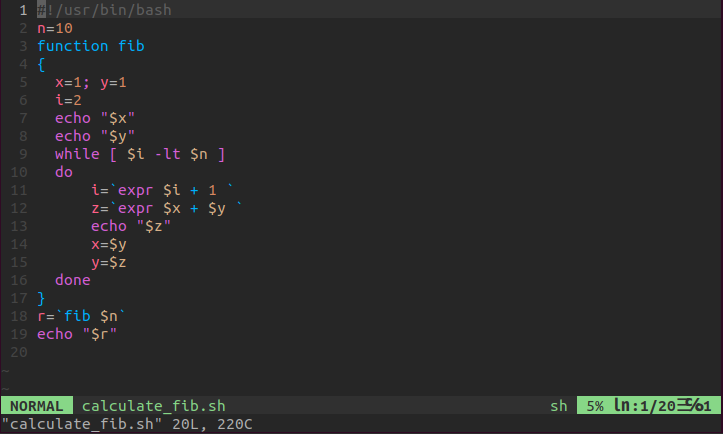
\includegraphics[width=4in]{chapters/part-1/figures/vim_fib.png}
	\caption{Vim (with user's profile customization as introduced in this chapter).}
\end{figure}

\begin{figure}[!htb]
	\centering
	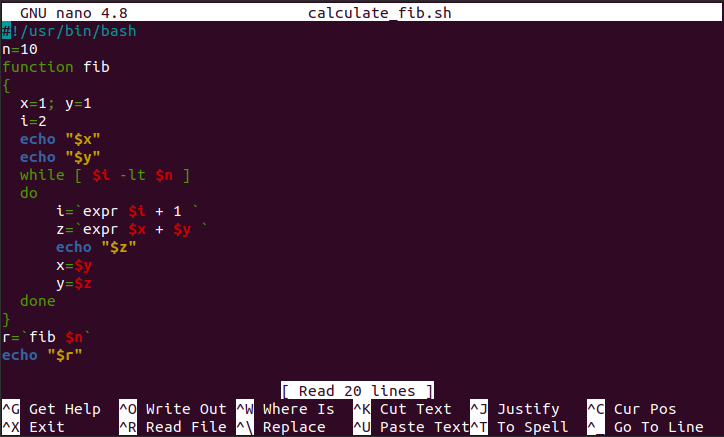
\includegraphics[width=4in]{chapters/part-1/figures/nano_fib.png}
	\caption{The nano editor.}
\end{figure}

\begin{figure}[!htb]
	\centering
	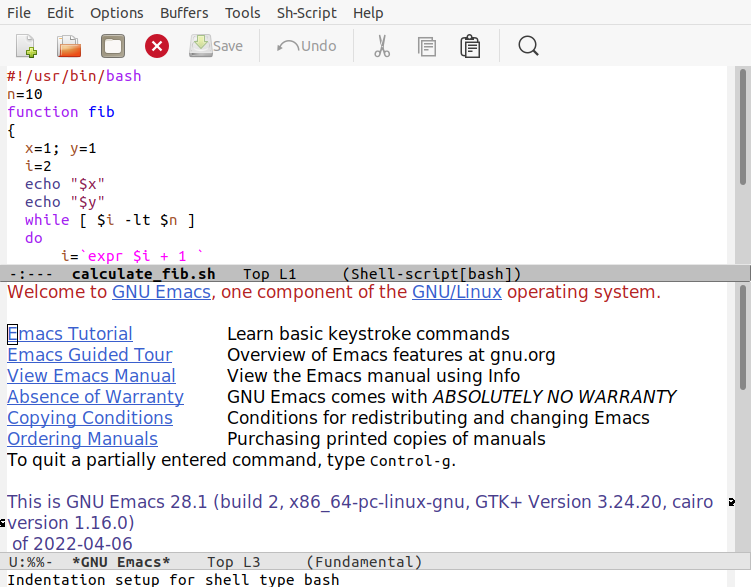
\includegraphics[width=4in]{chapters/part-1/figures/emacs_fib.png}
	\caption{The emacs editor.}
\end{figure}

\begin{figure}[!htb]
	\centering
	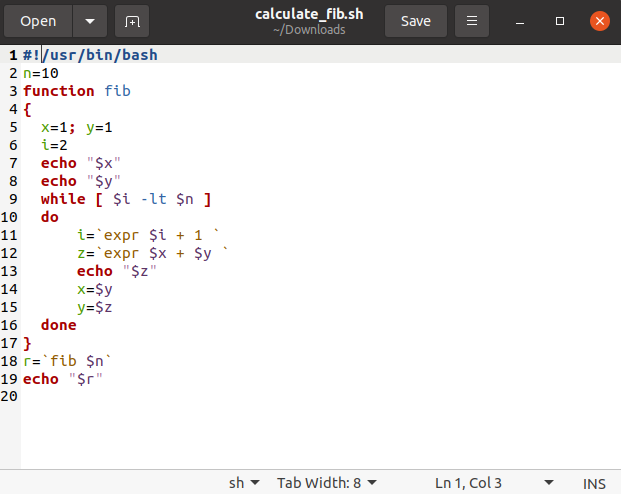
\includegraphics[width=4in]{chapters/part-1/figures/gedit_fib.png}
	\caption{The gedit editor.}
\end{figure}

\begin{figure}[!htb]
	\centering
	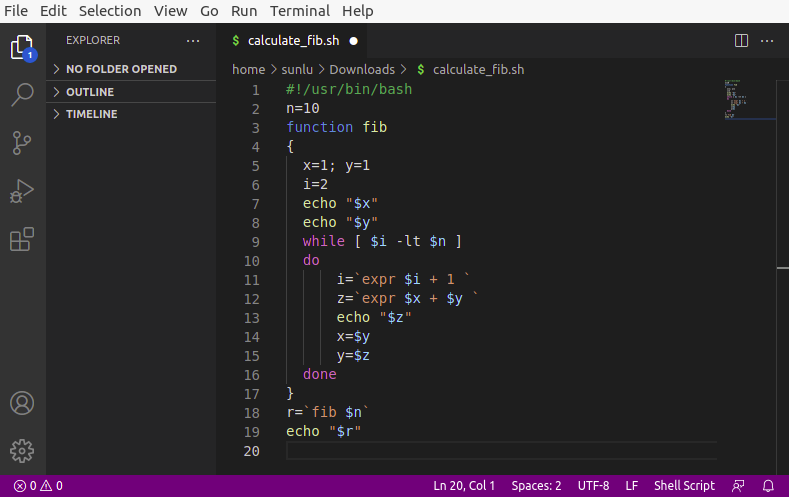
\includegraphics[width=4in]{chapters/part-1/figures/vscode_fib.png}
	\caption{Visual Studio Code.}
\end{figure}

%\chapterauthor{Author Name}{Author Affiliation}
%\chapterauthor{Second Author}{Second Author Affiliation}
\chapter{File Management} \label{ch:fm}

File management is a big portion of OS. In Linux, each device (such as a printer) is treated and managed as a file, and Linux uses a tree hierarchy to manage devices and files. This chapter introduces the filesystem hierarchy and commonly used file management commands.

\section{Filesystem Hierarchy Standard} \label{ch:fm:sec:hierarchy}

The root directory is denoted by a single forward slash ``\verb|/|''. All sub directories or files can be located by its full path, which looks like the following
\begin{lstlisting}
/<directory>/<subdirectory>/.../<directory-name>
/<directory>/<subdirectory>/.../<file-name>
\end{lstlisting}
where the first \verb|/| in each row represents the root directory, and sequential \verb|/| represents entering a subdirectory.

Upon Linux installation, a file hierarchy is created. A user can create new files under this hierarchy framework, but should not change the framework itself. The hierarchy is given in Fig. \ref{ch:fm:fig:hierarchy}. Notice that different Linux distributions may differ slightly on how the architecture looks like. The ``\verb|/|'' in the figure, as introduced, stands for the root directory, and ``\verb|root|'' in the figure is a subdirectory under \verb|/| whose directory name is ``root'' and it is used store root user related documents. They are two different directories.

\begin{figure}[htbp]
	\centering
	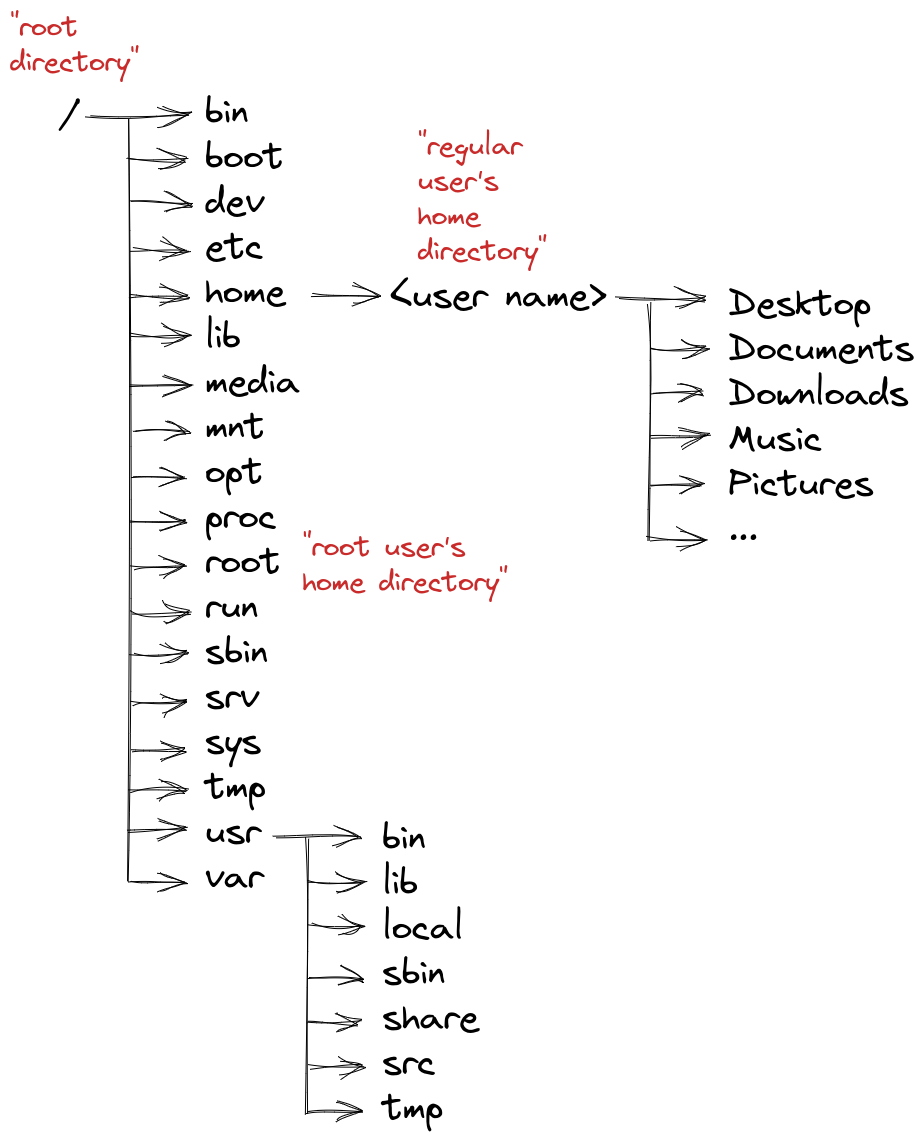
\includegraphics[width=250pt]{chapters/part-1/figures/linux_file_hierarchy.png}
	\caption{An example of Linux file system hierarchy.} \label{ch:fm:fig:hierarchy}
\end{figure}

A regular user's home directory is often located at \verb|/home/<user name>|. When logging in as a regular user, his home directory is stored in the HOME environment and can be retrieved by \verb|$HOME|. A shortcut to \verb|$HOME| is given by the tilde \verb|~| for convenience. Hence, for example \verb|ls ~| lists down the files and directories under his home directory.

As can be seen from Fig. \ref{ch:fm:fig:hierarchy}, the hierarchy contains quite a few pre-determined subdirectories, each serving a different purpose. For the ease of illustration, these subdirectories are roughly categorized by functionalities and accessibility shown in Fig. \ref{ch:fm:fig:directorycate}.

\begin{figure}[htbp]
	\centering
	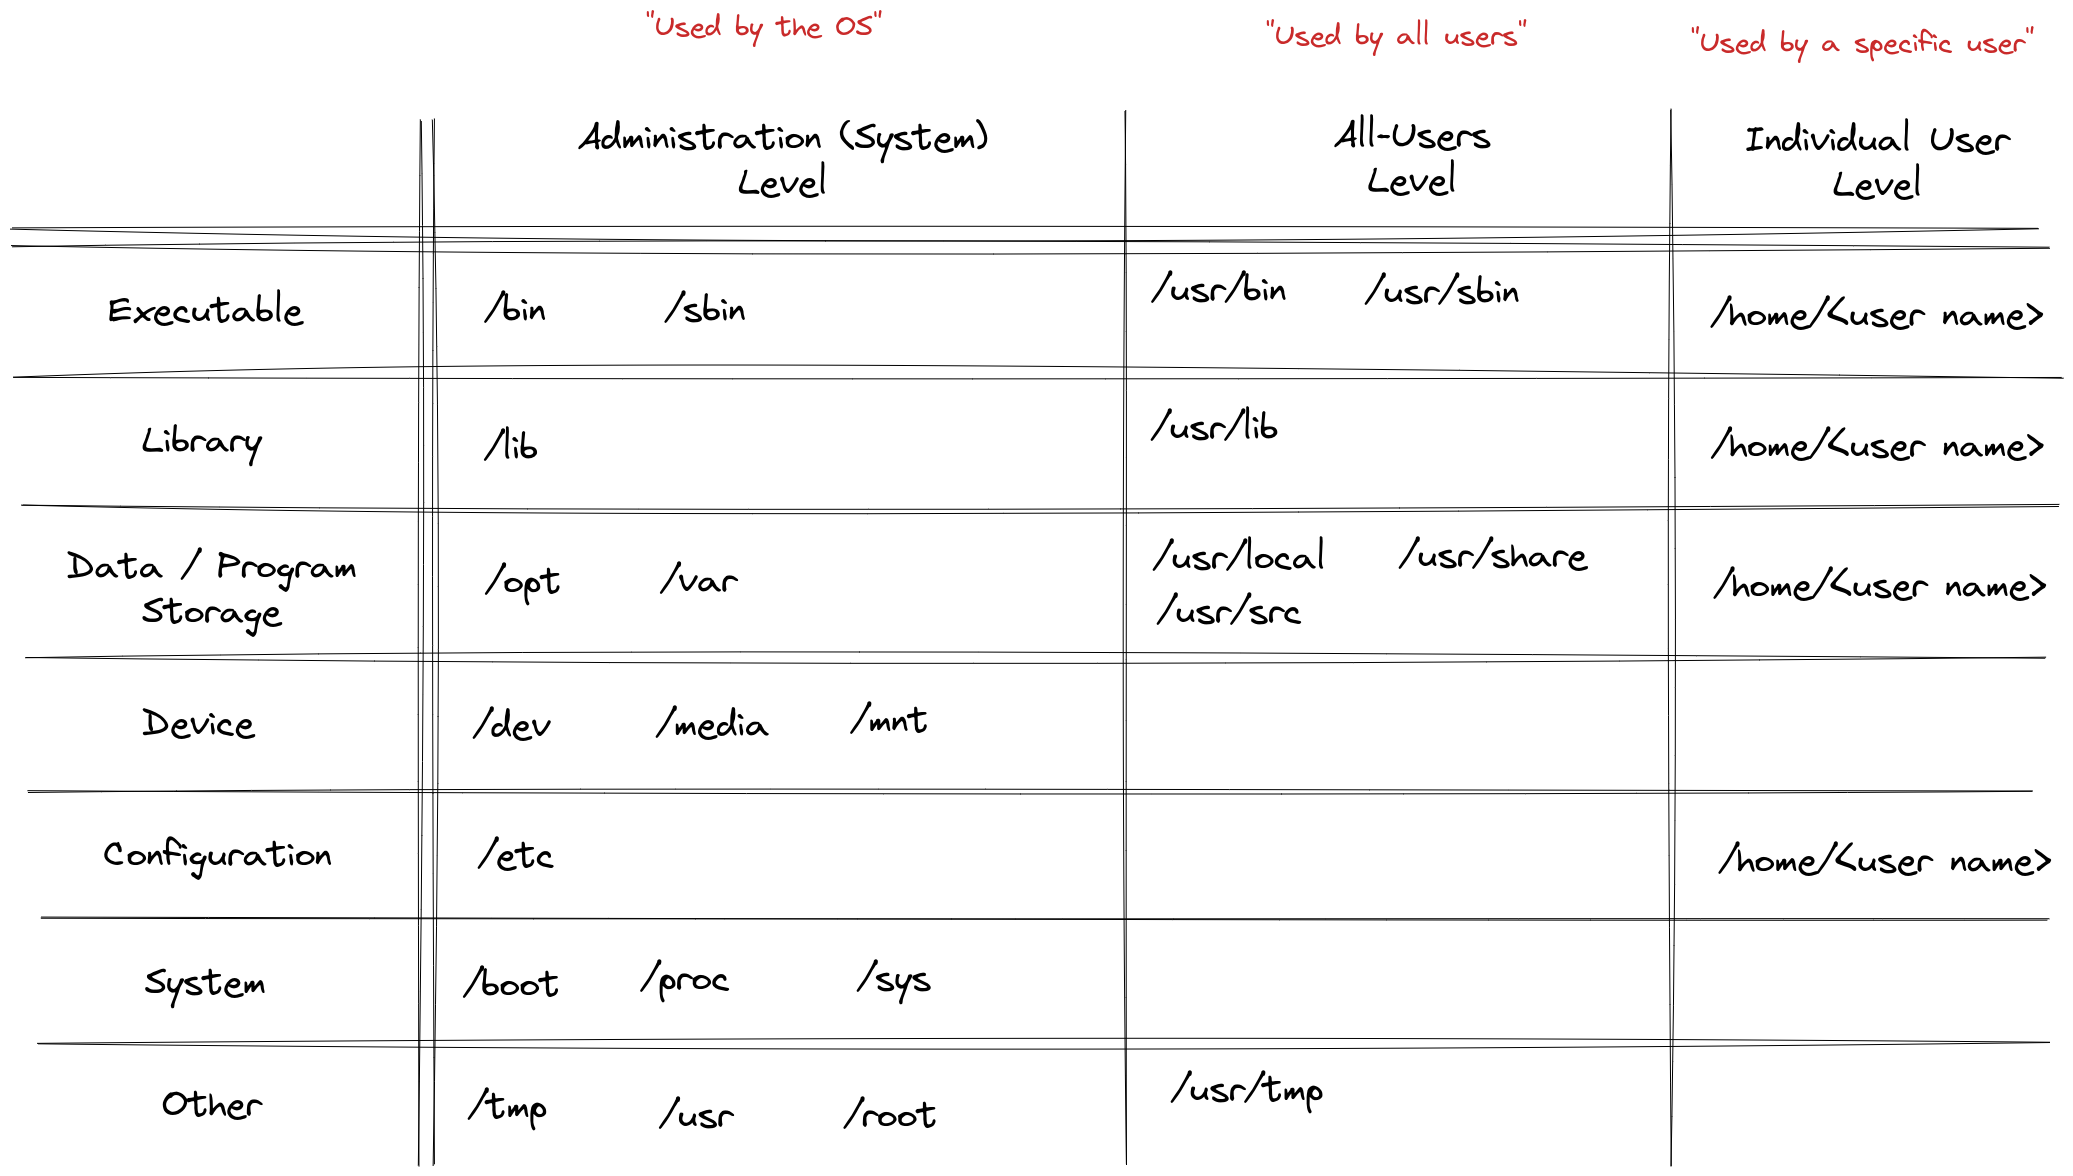
\includegraphics[width=350pt]{chapters/part-1/figures/linux_directory_cate.png}
	\caption{A rough categorization of commonly used directories in Linux file hierarchy standard.} \label{ch:fm:fig:directorycate}
\end{figure}

A brief introduction to the directories are summarized in Table \ref{ch:fm:tab:hierarchyintro}.

\begin{table}
  \centering \caption{Introduction to commonly used directories in Linux file hierarchy standard.}\label{ch:fm:tab:hierarchyintro}
  \begin{tabularx}{\textwidth}{lX}
    \hline
    Directory & Description \\ \hline
    \verb|/bin|, \verb|/sbin| & Executables used by the OS, the administrator, and the regular users. \\ 
    \verb|/lib| & Libraries to support \verb|/bin| and \verb|/sbin|. \\ 
    \verb|/usr/bin|, \verb|/usr/sbin| & Executables used by the administrator and the regular users. \\ 
    \verb|/usr/lib| & Libraries to support \verb|/usr/bin| and \verb|/usr/sbin|. \\ 
    \verb|/opt| & Application software installed by OS and administrator for all users. \\ 
    \verb|/var| & Directories of data used by applications. \\ 
    \verb|/usr/local| & Application software installed by administrator for all users. \\ 
    \verb|/usr/share| & Architecture-independent sharable text files for applications. \\ 
    \verb|/usr/src| & Source files or packages managed by software manager. \\ 
    \verb|/dev| & Files representation of devices, such as CPU, RAM, hard disks. \\ 
    \verb|/media| & System mounts of removable media. \\ 
    \verb|/mnt| & Manual mounts of devices. \\ 
    \verb|/etc| & Configuration files for OS, users, and applications. \\ 
    \verb|/boot| & Linux bootable kernel and initial setups. \\ 
    \verb|/proc| & System resources information. \\ 
    \verb|/sys| & Linux kernel information, including a mirror of the kernel data structure. \\ 
    \verb|/tmp|, \verb|usr/tmp| & Temporary files. \\ 
    \verb|/root| & Root user's home directory. \\ 
    \verb|/home/<user name>| & A regular user's home directory, containing executables, configurations and files specifically belong to this user. \\
    \hline
  \end{tabularx}
\end{table}

Linux file hierarchy standard differs from MS-DOS and Windows in several ways. Firstly, Linux stores all files (regardless of their physical location) under the root directory, while Windows uses drive letters such as \verb|C:\|, \verb|D:\| to distinguish different hard drives. Secondly, Linux uses slash (\verb|/|) to separate directory names, e.g. \verb|/home/username| while Windows uses back slash (\verb|\|), e.g. \verb|C:\Users\username|. Lastly, Linux uses ``magic numbers'' to indicate file types, while Windows often uses suffixes to tell file types. 

Magic numbers of a file refer to the first few bytes of a file that are unique to a particular file type, for example, PNG file is hex \verb|89 50 4e 47|. Linux compare the magic numbers of a file with an internal database to decide the file types and features. Distinguishing file types using magic numbers can be more reliable than using suffixes, though a bit less intuitive.

\section{Commonly Used File Exploring Commands} \label{ch:fm:sec:filemanagement}

Some of the most widely used file exploring and managing commands are summarized in Table \ref{ch:fm:tab:commonfilecommands}. Notice that \verb|chmod| and \verb|chown| are administration related commands that change the accessibility of a directory or a file, and will be introduced in a later sections together with the Linux permission system. The rest commands are categorized and introduced in the following subsections.

\begin{table}
  \centering \caption{Commonly used commands to navigate in the Linux file system.}\label{ch:fm:tab:commonfilecommands}
  \begin{tabularx}{\textwidth}{lX}
    \hline
    Command & Description \\ \hline
    \verb|pwd| & Print working directory. \\ 
    \verb|ls| & List the subdirectories and files (and their detail information) in a given directory. \\ 
    \verb|touch| & Create an empty file. \\ 
    \verb|mkdir| & Create an empty subdirectory. \\ 
    \verb|mv| & Move (cut-and-paste) a directory or a file; change name of a directory or a file. \\ 
    \verb|cp| & Copy-and-paste a directory or a file. \\ 
    \verb|rm|, \verb|rmdir| & Remove a directory or a file (not to Trash, but just gone). \\ 
    \verb|chmod| & Change permission. \\ 
    \verb|chown| & Change ownership. \\
    \hline
  \end{tabularx}
\end{table}

\subsection{Print Working Directory}

As given in Table \ref{ch:sb:tab:shellenvironmentvars}, \verb|$PWD| is the environmental variables to store the current working directory of the shell. Therefore, to print the current working directory in the console, use command 
\begin{lstlisting}
$ echo $PWD
\end{lstlisting}
Alternatively, use \verb|pwd| as follows which has the same effect.
\begin{lstlisting}
$ pwd
\end{lstlisting}

\subsection{List Information about Files and Directories}

As one of the most frequently used commands, \verb|ls| lists down information about the files and subdirectories in the selected directory, and by default sort the entries alphabetically. The syntax is given below.
\begin{lstlisting}
$ ls [<option>] [<path>]
\end{lstlisting}

An example is given in Fig. \ref{ch:fm:fig:lscommandexample}. As shown in the example, command \verb|ls| alone shows only the name of files and subdirectories excluding hidden items and details of each item. With the additional arguments in the option field, the returns can be customized with more details displayed. For example in Fig. \ref{ch:fm:fig:lscommandexample}, the \verb|-l| argument displays the information in long listing form, which includes the owner and access control list information. More details about files and directories access control list are given in later part of this section.

\begin{figure}[htbp]
	\centering
	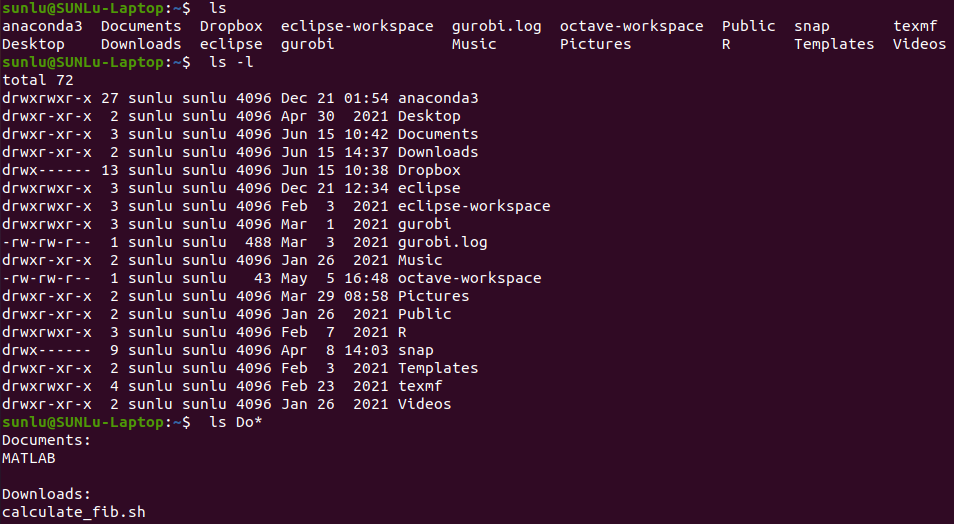
\includegraphics[width=350pt]{chapters/part-1/figures/ls_command_example.png}
	\caption{List down information of files and subdirectories in the current working directory.} \label{ch:fm:fig:lscommandexample}
\end{figure}

More information can be found in the \verb|ls| command manual which is accessible via \verb|ls --help|. Some commonly used \verb|ls| arguments are summarized in Table \ref{ch:fm:tab:lscommandargument}. It is also possible to combine the options. For example, \verb|ls -al| aggregates the effects of using \verb|ls -a| and \verb|ls -l|.

\begin{table}[htbp]
  \centering \caption{Commonly used arguments and their effects for \textit{ls} command.}\label{ch:fm:tab:lscommandargument}
  \begin{tabularx}{\textwidth}{lX}
    \hline
    Directory & Description \\ \hline
    \verb|-a|, \verb|--all| & Include hidden files and subdirectories in the display, including current directory ``\verb|.|'' and parent directory ``\verb|..|'' in the list. \\ 
    \verb|-A|, \verb|--almost-all| & Include hidden files and subdirectories in the display, excluding ``\verb|.|'' and ``\verb|..|''. \\ 
    \verb|-C|, \verb|--color[=WHEN]| & Colorize the output. \\ 
    \verb|-l| & Use a long listing format. \\ 
    \verb|-s|, \verb|--size| & Print the allocated size of each file, in blocks. \\ 
    \verb|-S| & Sort the displayed content. \\ 
    \verb|-t| & Sort by modification time. \\
    \hline
  \end{tabularx}
\end{table}

Notice that some Linux distributions may come by default an alias about \verb|ls|, which usually helps to displays the information in a clearer manner. For example, when \verb|ls='ls --color-auto'| is used, the displayed content will be colored based on the type of the files and subdirectories.

\subsection{Create Files and Directories}

The \verb|touch| command is used to update timestamps of a file. If the file does not exist, \verb|touch| will create that file with empty content. Hence, it is often used to create empty files. To do so, simply use \verb|touch| followed by the full path to the file as follows.
\begin{lstlisting}
$ touch [<option>] <path>
\end{lstlisting}
For example,
\begin{lstlisting}
$ touch ~/test
\end{lstlisting}
will create an empty file ``\texttt{test}'' under the user's home directory. If only the name of the file is given, it will by default create the file under the current working directory. Notice that if a file name starts with ``\verb|.|'', it will be treated as a hidden file or automatically.

\verb|touch| can also be used to create multiple files in a single-line command. For example,
\begin{lstlisting}
$ touch test1 test2
\end{lstlisting}
creates both \texttt{test1} and \texttt{test2} in the current working directory.

To create a file containing a single line of string, consider using \verb|echo| command with \verb|>| as follows. It is more convenient than using \textit{Vim} for the same task, although also possible.
\begin{lstlisting}
$ echo '<content>' > <path>
\end{lstlisting}
For example,
\begin{lstlisting}
$ echo '<html><body><h1>Hello world!</h1></body></html>' > ~/test.html
\end{lstlisting}
creates a simple static HTML web page that says ``Hello world!'' in the home directory.

Similar with \verb|touch|, use \verb|mkdir| followed by the path of the directory (including directory name) to create a directory as follows.
\begin{lstlisting}
$ mkdir [OPTION] <path>
\end{lstlisting}
Specifically, \verb|-p| option of \verb|mkdir| allows it to create nested directories along the given path if the directories do not exist.

\subsection{Move, Copy-and-Paste, and Remove Files and Directories}

To move a file or a directory from an existing directory to another, simply use \verb|mv| command as follows.
\begin{lstlisting}
$ mv [<option>] <source> <target>
\end{lstlisting}
Different from the conventional cut-and-paste, while moving the item, it is possible to also rename the item simultaneously. For example,
\begin{lstlisting}
$ mv ~/dog.png ~/Pictures/puppy.png
\end{lstlisting}
will not only move the file \verb|dog.png| in the home directory to the subdirectory \verb|Pictures|, but also chance the file name to \verb|puppy.png|. For this reason, \verb|mv| can also be used to rename an item rather than moving the item, just by ``move'' it to the same directory but with a different name.

Some commonly used arguments of \verb|mv| is summarized in Table \ref{ch:fm:tab:mvcpcommandargument}, many of which concerns about the case where there is already an existing item with the identical name in the target path.

\begin{table}
  \centering \caption{Commonly used arguments and their effects for \texttt{mv} and \texttt{cp} commands.}\label{ch:fm:tab:mvcpcommandargument}
  \begin{tabularx}{\textwidth}{lX}
    \hline
    Directory & Description \\ \hline
    \verb|-b| & Make a backup before overwrite. \\ 
    \verb|-u| & Overwrite only when source target item is newer than the target path item. \\ 
    \verb|-i| & Prompt before overwrite. \\ 
    \verb|-f| & Do not prompt before overwrite. \\
    \hline
  \end{tabularx}
\end{table}

The copy-and-paste command \verb|cp| works similar with the move command \verb|mv|, except that it will not remove the item from the source path. Similar syntax applies to \verb|cp| as follows, and arguments in Table \ref{ch:fm:tab:mvcpcommandargument} also apply to \verb|cp|.
\begin{lstlisting}
$ cp [<option>] <source> <target>
\end{lstlisting}

To permanently delete an item, use \verb|rm| command as follows.
\begin{lstlisting}
$ rm [<option>] <path>
\end{lstlisting}
For safety, when using \verb|rm| the OS will keep prompting messages asking user to confirm whether to permanently delete an item or not. In some OS setups, it is by default forbidden to delete a directory unless it is empty. The following arguments in Table \ref{ch:fm:tab:rmcommandargument} can be used to change the setup.

\begin{table}
  \centering \caption{Commonly used arguments and their effects for \texttt{rm} command.}\label{ch:fm:tab:rmcommandargument}
  \begin{tabularx}{\textwidth}{lX}
    \hline
    Directory & Description \\ \hline
    \verb|-f| & Ignore nonexistent files and arguments and do not prompt. \\ 
    \verb|-r| & Remove directories and their contents recursively. \\ 
    \verb|-i| & Prompt before every removal. \\ 
    \verb|-d| & Remove empty directories. \\
    \hline
  \end{tabularx}
\end{table}

It is possible though, that removed items using \verb|rm| be recovered by expertise. For greater assurance that the deleted contents are truly unrecoverable, consider using \verb|shred| which can physically overwrite the portion of hardware drive where the item is located. More details of \verb|shred| can be found by
\begin{lstlisting}
$ shred --help
\end{lstlisting}

\subsection{Use of Wildcard Characters}

When performing actions such as listing, moving, copying, removing, wildcard characters can be used in the path. For example, \verb|ls a*| lists all items in the current directory that starts with letter ``a''. Commonly used meta-characters are summarized in Table \ref{ch:fm:tab:metacharacters}.

\begin{table}
  \centering \caption{Commonly used wildcard characters.}\label{ch:fm:tab:metacharacters}
  \begin{tabularx}{\textwidth}{lX}
    \hline
    Directory & Description \\ \hline
    \verb|*| & Matches any number of characters. \\ 
    \verb|?| & Matches one character. \\ 
    \verb|[...]| & Matches characters given in the square bracket, which can include a hyphen-separated range of characters. \\
    \hline
  \end{tabularx}
\end{table}

\section{Access Control List} \label{ch:fm:sec:accesscontrollist}

Each file or directory in the Linux OS is assigned with an owner and a permission list known as the Access Control List (ACL). ACL prevents unauthorized entities to access an item. The ACL of a file can be viewed using \verb|ls -l|. An example has been given in Fig. \ref{ch:fm:fig:lscommandexample} in the earlier section.

The first column of the output in Fig. \ref{ch:fm:fig:lscommandexample} gives the type and permission of the item. The leading \verb|d| and \verb|-| indicate subdirectory and regular file respectively. Other commonly seen indicators are \verb|l| for a symbolic link, \verb|b| for a block device, \verb|c| for a character device, \verb|s| for a socket and \verb|p| for a named pipe.

Following the item type indicator is the ACL of the item in the form of 9-bit permission that looks like \verb|rwxrwxrwx|. The characters \verb|r|, \verb|w| and \verb|x| stand for three types of permissions ``read'', ``write'' and ``execute'' respectively. An explanation to these permissions is summarized in Table \ref{ch:fm:tab:threepermissions} and more details can be found in the \verb|ls| command manual accessible using \verb|ls --help|. The 9-bit permission of an item indicates the permissions of 3 types of users to the item, the first 3 bits the file owner, the middle 3 bits the file group, and the last 3 bits other users. If any bit in the 9-bit permission is overwritten by a dash \verb|-|, it means that the associated permission for the associated users is banned.

\begin{table}
  \centering \caption{Three types of permissions.}\label{ch:fm:tab:threepermissions}
  \begin{tabularx}{\textwidth}{lX}
    \hline
    Directory & Description \\ \hline
    \verb|r| & View what is in the file or directory. \\ 
    \verb|w| & Change file contents; rename file; delete file. Add or remove files or subdirectories in a directory. \\ 
    \verb|x| & Run a file as a program. Change to the directory as the current directory; search through the directory; access metadata (file size, etc.) of files in the directory. \\
    \hline
  \end{tabularx}
\end{table}

Commands \verb|chown| and \verb|chmod| can be used to change the ownership and ACL of an item respectively. Details are given in the following subsections.

\subsection{Change Ownership and Group of a File or Directory}

Administrative privilege is required to run \verb|chown| command to change the ownership and group of a file or a directory as follows.
\begin{lstlisting}
# chown [<option>] <new_owner>[:<new_group>] <path>
\end{lstlisting}
For example, in Fig. \ref{ch:fm:fig:chownexp},
\begin{lstlisting}
$ sudo chown root:root calculate_fib.sh
\end{lstlisting}
is used to change the ownership and group of file \verb|calculate_fib.sh| from \verb|sunlu| to \verb|root|. Notice that elevated privilege is required to change its ownership, otherwise the request will be rejected as shown in Fig. \ref{ch:fm:fig:chownexp}.

\begin{figure}[htbp]
	\centering
	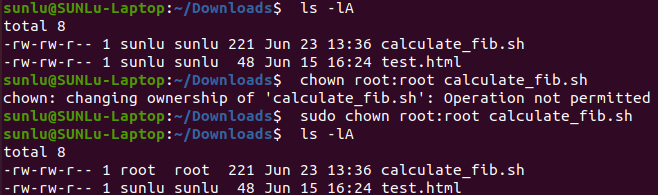
\includegraphics[width=350pt]{chapters/part-1/figures/chownexp.png}
	\caption{Change ownership and group of a file.} \label{ch:fm:fig:chownexp}
\end{figure}

\subsection{Change Permissions of a File or Directory}

Both the owner and the users with administrative privilege can change the ACL of a file or directory using \verb|chmod| as follows. The ACL, in this context, is called the mode of the item.
\begin{lstlisting}
$ chmod [<option>] <new_mode> <path>
\end{lstlisting}
For example, in Fig. \ref{ch:fm:fig:chmodexp}, \verb|g-w| is used to subtract ``writing'' permission from ``group'', and \verb|go+w| is used to add ``writing'' permission to `group'' and ``other'', respectively. Here, \verb|u|, \verb|g| and \verb|o| represents ``user'' (owner), ``group'' and ``other'', and \verb|r|, \verb|w| and \verb|x|, ``read'', ``write'' and ``execute'', respectively.
\begin{figure}[htbp]
	\centering
	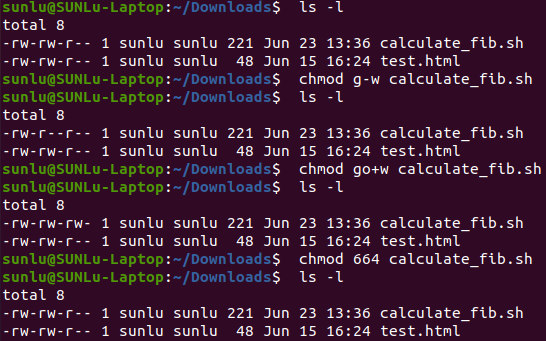
\includegraphics[width=350pt]{chapters/part-1/figures/chmodexp.png}
	\caption{Change 9-bit permission (mode) of a file.} \label{ch:fm:fig:chmodexp}
\end{figure}
Alternatively, 3-digit numbers such as \verb|664| as shown in Fig. \ref{ch:fm:fig:chmodexp} can also represent a permission. The first digit is associated with the permission given to the ``user'', where in this example \verb|6| (\verb|110B|) represents \verb|rw-|. Each ``1'' in the binary number is associated with a permission. The second and third digits are associated with the permission given to ``group'' and ``other'' respectively. Hence, \verb|664| would assign \verb|rw-rw-r--| to the file.

\subsection{Change Default Permissions}

The default ACL for a newly created file or directory is defined by \verb|umask|. Check its value by
\begin{lstlisting}
$ umask
\end{lstlisting}
And change its value temporarily in the opening shell by
\begin{lstlisting}
$ umask <new value>
\end{lstlisting}

The value of \verb|umask|, after converting to binary, represents the bits in the 9-bit permission system that is disabled. For example, a \verb|umask| value of \verb|002| represents \verb|rwxrwxr-x| in the 9-bit permission system, because the binary form of \verb|002|, \verb|000000010|, blocks the $8$-th bit in the permission.

To permanently change the value of \verb|umask|, configure it in \verb|.bashrc| as introduced in Section \ref{ch:sb:subsec:customizeshell}.

\section{Search through the System}

The most frequently used 3 searching actions are as follows.
\begin{itemize}
  \item Look for the location of a command using its name
  \item Look for the location of a file using its name (and other metadata such as size, permission, etc.)
  \item Look for the location of a file using a portion its content
\end{itemize}

Many approaches can be used to achieve the goals, some of which are introduced as follows.

\subsection{Look for a Command}

Use \verb|type| to look for a command as follows.
\begin{lstlisting}
$ type <command>
\end{lstlisting}

For example
\begin{lstlisting}
$ type cd
cd is a shell builtin
$ type python
python is /usr/bin/python
$ type ls
ls is aliased to `ls --color=auto'
\end{lstlisting}

\subsection{Looking for Files by Metadata}

Many Linux distributions come with built-in command \verb|locate| that can be used to quickly locate a file by (a fraction of) its path as follows. Notice that as long as a file or directory's full path contains the searched content, there is a chance that it will appear in the result. As a result, if the name of a directory is used for searching, all the items in that directory will likely to appear in the result (as their full paths contain the name of the directory).
\begin{lstlisting}
$ locate <file or path fraction>
\end{lstlisting}

The mechanism of \verb|locate| is explained as follows. The OS runs \verb|updatedb| in the background usually once a day to update an internal database that gathers the names of files, and \verb|locate| searches that database for the file. Notice that \verb|locate| may fail to find recently added files if it has not been added to the database by \verb|updatedb|. Besides, not all files' name are stored in that database by default, and a configuration file at \verb|/etc/updatedb.conf| determines which files' name to be included. It is also worth mentioning that it will take some time to run \verb|updatedb| for the first time, as it has a lot of things to add to the database during its initial run.

One may get confused by commands \verb|locate| and \verb|mlocate|. The two commands are very similar and they differ only beyond basic usage. Sometimes \verb|locate| is aliased to \verb|mlocate| when both functions are installed. In the scope of our discussion, we do not distinguish \verb|locate| and \verb|mlocate|.

An example of using \verb|locate|/\verb|mlocate| is given in Fig. \ref{ch:fm:fig:locateexp}. It can be seen from this example that the searching is done globally and does not rely on the current working directory.
\begin{figure}[htbp]
	\centering
	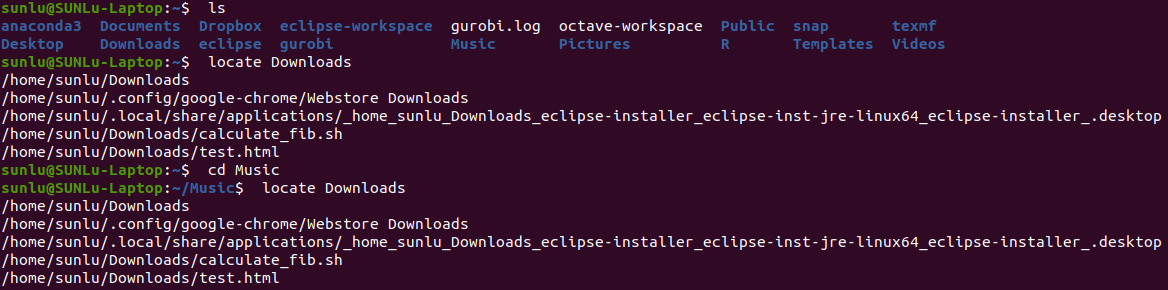
\includegraphics[width=350pt]{chapters/part-1/figures/locateexp.png}
	\caption{Search for files and directories using \textit{locate}.} \label{ch:fm:fig:locateexp}
\end{figure}

\subsection{Looking for Files by Variety of Properties}

It is worth mentioning that for safety and privacy reasons, \verb|mlocate| only shows the items that the user would be able to detect manually using \verb|cd| and \verb|ls| in the first place. Therefore, a regular user cannot locate any file under \verb|/root| our other users' home directory using this method.

A more common and widely accepted way of looking for a file by its variety of attributes is using \verb|find| as follows.
\begin{lstlisting}
$ find [<options>] [<path>] <expression>
\end{lstlisting}

The \verb|<options>| argument can be used to configure how the symbolic links should be handled. Symbolic links are like shortcut in Windows PC. It is a link that points to other directories of files. If \verb|-P| (default option) is used, the symbolic links are treated as the links themselves, but not the files they are linking to, whereas \verb|-L| does the opposite. Debugging modes and query optimization can also be enabled from \verb|<options>|. The \verb|<path>| argument specifies the directory from where the query is conducted. The \verb|<expression>| argument specifies the keyword and the query method.

The following are examples of using \verb|find| in different scenarios. The examples are taken from RedHat at \cite{redhat2022find}.

\vspace{0.1in}
\noindent \textbf{List everything in a directory and its subdirectories}
\vspace{0.1in}

\begin{lstlisting}
$ find ~/Documents -ls
3554235 0 drwxr-xr-x [...] 05:36 /home/seth/Documents/
3554224 0 -rw-rw-r-- [...] 05:36 /home/seth/Documents/Foo
3766411 0 -rw-rw-r-- [...] 05:36 /home/seth/Documents/Foo/foo.txt
\end{lstlisting}

\vspace{0.1in}
\noindent \textbf{Find files by name}
\vspace{0.1in}

Case sensitive: \verb|-name|
\begin{lstlisting}
$ find / -name "*Foo*txt" 2>/dev/null
/home/seth/Documents/Foo.txt
\end{lstlisting}

Case insensitive: \verb|-iname|
\begin{lstlisting}
$ find / -iname "*Foo*txt" 2>/dev/null
/home/seth/Documents/Foo.txt
/home/seth/Documents/foo.txt
/home/seth/Documents/foobar.txt
\end{lstlisting}

Wildcards such as \verb|*| can be used. Commonly used wildcards are given in Table \ref{ch:fm:tab:metacharacters}.

\vspace{0.1in}
\noindent \textbf{Find files by the content}
\vspace{0.1in}

\begin{lstlisting}
$ find ~/Documents/ -name "*txt" -exec grep -Hi penguin {} \;
/home/seth/Documents/Foo.txt:I like penguins.
/home/seth/Documents/foo.txt:Penguins are fun.
\end{lstlisting}
where in this example, \verb|-exec| allows executing a command to the findings. Notice that \verb|grep| by itself can also be used to search files by contents.

\vspace{0.1in}
\noindent \textbf{Find files by type}
\vspace{0.1in}

To find all files,
\begin{lstlisting}
$ find ~ -type f
/home/seth/.bash_logout
/home/seth/.bash_profile
/home/seth/.bashrc
/home/seth/.emacs
/home/seth/.local/share/keyrings/login.keyring
/home/seth/.local/share/keyrings/user.keystore
/home/seth/.local/share/gnome-shell/gnome-overrides-migrated
\end{lstlisting}
Specifically, to find empty files,
\begin{lstlisting}
$ find ~ -type f -empty
random.idea.txt
\end{lstlisting}

To find all subdirectories,
\begin{lstlisting}
$ find ~/Public -type d
find ~/Public/ -type d
/home/seth/Public/
/home/seth/Public/example.com
/home/seth/Public/example.com/www
/home/seth/Public/example.com/www/img
/home/seth/Public/example.com/www/font
/home/seth/Public/example.com/www/style
\end{lstlisting}

Use \verb|-maxdepth| to set the searching depth as follows.
\begin{lstlisting}
$ find ~/Public/ -maxdepth 1 -type d
/home/seth/Public/
/home/seth/Public/example.com
\end{lstlisting}

\vspace{0.1in}
\noindent \textbf{Find files by the timestamp it was accessed / changed / metadata changed}
\vspace{0.1in}

To find files whose latest modified time is at least 30 days ago (30 days ago or earlier), use
\begin{lstlisting}
 find /var/log -mtime +30
\end{lstlisting}
where \verb|-atime|, \verb|-ctime| and \verb|-mtime| search based on the number of days since each file was accessed, changed or had its metadata changed respectively. The alternatives \verb|-amin|, \verb|-cmin| and \verb|-mmin| work similarly in minutes. The \verb|+| indicates ``at least'' whereas \verb|-| indicates ``not more than''.

\section{File Archive}

The \verb|tar|, \verb|gzip| and \verb|zip| commands can all be used in files archive, but with different features, as given in Table \ref{ch:fm:tab:filearchivetools}.

\begin{table}
	\centering \caption{Commonly used file archive tools.}\label{ch:fm:tab:filearchivetools}
	\begin{tabularx}{\textwidth}{lX}
		\hline
		Directory & Description \\ \hline
		\verb|tar| & Save many files together into a single tape or disk archive, and can
		restore individual files from the archive. By default, it does not compress the files. However, \verb|-z| option can be used in combination of the command to add compression feature. \\ 
		\verb|gzip| & Compress or restore files. \\ 
		\verb|zip| & Compress multiple files one-by-one and integrate them together into a single file. \\
		\hline
	\end{tabularx}
\end{table}

Only \verb|tar| command is introduced here, as it is the most commonly used one among the three, and it can satisfy most use cases. A common way of using \verb|tar| is as follows. Use
\begin{lstlisting}
$ tar -cvzf <archive-file> <file1> <file2> <file3> ...
\end{lstlisting}
to archive and zip files, and
\begin{lstlisting}
$ tar -xvzf <archive-file>
\end{lstlisting}
to restore files from the archive file. The commonly used archive file name, in this scenario, is \verb|<filename>.tgz|.

The detailed explanation to all available options for \verb|tar| can be found using \verb|tar --help|. The most commonly used options are \verb|-c|, \verb|-x|, \verb|-z|, \verb|-f| and \verb|-v|, standing for creating compress tape, extracting (restoring) file, adding compressing feature, using file archive, and listing processed files in the console, respectively.
















\chapter{Software Management}

Linux as an OS monitors and maintains the software installed on the system. Different Linux distributions may use different tools to manage the software.

\section{Tasks and Approaches}

The OS should support at least the following tasks.
\begin{itemize}
	\item Install software.
		\begin{itemize}
			\item Install software from the installation package.
			\item If possible, automatically find and download the installation package.
			\item If possible, automatically find, download and install all the dependencies.
		\end{itemize}
	\item Query software.
		\begin{itemize}
			\item Query the software already installed on the system.
			\item If possible, query software online.
		\end{itemize}
	\item Remove software.
	\item Update software.
\end{itemize}

In Linux, software information (dependencies, version, instruction to installation, etc.) are stored in special data structures known as packages. When installing a software, the OS locates the packages and install them according to the instructions that comes with the packages. The OS also traces the software it has installed, monitors their behaviors, performs updates or uninstalls per requested by the user. Different Linux distributions may use different package formats and package management tools. The most well-known ones include:
\begin{itemize}
	\item RPM
	\item \myabb{Debian Package Manager}{DEB}
\end{itemize}
Note that RPM and DEB can refer to both the package formats and the package managing tools. There are proponents on both sides of RPM versus DEB, and both of them are very popular tools in different Linux distributions.

Linux kernel is also a software and needs to be monitored and updated from time to time. Linux kernel management is also briefly introduced in this chapter. Notice that advanced kernel management such as kernel customization goes beyond the scope of this notebook, hence are not included in this chapter.

\section{RPM Package}

\mync{RPM} (\verb|.rpm|) is the preferred package format for Red-Hat-based distributions such as RHEL, Fedora, CentOS and Oracle Linux. It uses \verb|rpm| command to mange RPMs. In a later stage, other tools such as \verb|yum| and \verb|dnf| have been added to the library for better user experience and enhanced RPM facility. 

\subsection{Brief Introduction}

RPM contains rich information, including not only the payload of the software such as commands, configuration files, libraries and documentation, but also metadata such as the source of the package, dependencies, etc.

The name of an RPM should follow the protocol and by itself contains important information about the software. An example is given below. Use \verb|rpm -q| followed by the software name \verb|python3| to query the package as follows. If the package is installed, its full name should be returned.
\begin{lstlisting}
$ rpm -q python3
python3-3.9.18-3.el9_4.1.x86_64
\end{lstlisting}
where in this example the name of the software is \verb|python3|, the version \verb|3.39.18|, the release (build) \verb|4.el9_4.1| with release number \verb|4|, distribution \verb|el9_4| and patch number \verb|1|, and finally architecture \verb|x86_64|. When the package is stored on the machine, it should also come with the suffix \verb|.rpm|. 

To retrieve more details, use \verb|rpm -qi| instead and
\begin{lstlisting}
$ rpm -qi python3
Name        : python3
Version     : 3.9.18
Release     : 3.el9_4.1
Architecture: x86_64
Install Date: Tue 09 Jul 2024 12:48:28 PM +08
Group       : Unspecified
Size        : 33021
License     : Python
Signature   : RSA/SHA256, Tue 21 May 2024 06:30:22 AM +08, Key ID 199e2f91fd431d51
Source RPM  : python3.9-3.9.18-3.el9_4.1.src.rpm
Build Date  : Fri 17 May 2024 10:49:06 PM +08
Build Host  : x86-64-03.build.eng.rdu2.redhat.com
Packager    : Red Hat, Inc. <http://bugzilla.redhat.com/bugzilla>
Vendor      : Red Hat, Inc.
URL         : https://www.python.org/
Summary     : Python 3.9 interpreter
Description :
Python 3.9 is an accessible, high-level, dynamically typed, interpreted
programming language, designed with an emphasis on code readability.
It includes an extensive standard library, and has a vast ecosystem of
third-party libraries.
...
\end{lstlisting}
can be retrieved.

\subsection{Package Management Using \texttt{rpm}}

An RPM package is required to install the software. An RPM package comes from the upstream software provider, who collects source codes, binary files, and other data, builds the software, and signs the package.

The command \verb|rpm| can be used to install the software from an RPM package. Note that installing software using \verb|rpm| requires the precise location of the RPM package and all dependencies to be installed in advance, which can be inconvenient. The \verb|rpm| command can also be used to validate, query, update, and remove software.

When a package is installed on the machine, its information is saved in the RPM database managed by the OS.

\subsection{Package Management Using \texttt{yum} and \texttt{dnf}}

Due to the drawbacks of \verb|rpm| mentioned earlier, other tools have been developed to handle package upstream repositories and dependencies more conveniently. These tools are YUM and its next generation \myabb{Dandified YUM}{DNF}, with their corresponding commands \verb|yum| and \verb|dnf| respectively.

YUM and DNF introduce the concept of repositories, allowing RPM packages to be part of a larger software ``package tree''. It becomes the publisher's responsibility to ensure that all the dependencies of the RPM can be traced from the repositories. If a dependency is not present, YUM and DNF can search the repositories to find the dependencies and install them together. When the user wants to install an RPM that has not been downloaded onto the machine, YUM and DNF can search the repositories for the RPM, download, and install it automatically. As a result, the user does not need to manually install all the dependencies or find and download the RPM themselves. In this sense, YUM and DNF can be taken as a wrapper of \verb|rpm| that come with additional features such as repository resolution and package retrieval. They run \verb|rpm| internally once the packages have been downloaded to the machine.

DNF is a further improvement of YUM with better dependency resolution and less memory usage. In many occasions, command \verb|yum| can be replaced by \verb|dnf| seamlessly. In some Linux distributions such as RHEL 9, \verb|yum| is used as an alias for \verb|dnf|. In the remaining part of the section, only DNF is discussed.

The basic syntax of DNF is
\begin{lstlisting}
$ dnf <operation> <package>
\end{lstlisting}
where \verb|<operation>| include
\begin{itemize}
	\item \verb|install|: install a package
	\item \verb|remove|: remove a package
	\item \verb|search|: search the repositories for a package
	\item \verb|autoremove|: remove dependencies packages irrelevant to currently installed program
	\item \verb|check-update|: check updates of packages from the repositories without downloading or installing the updates
	\item \verb|downgrade|: revert to a previous version
	\item \verb|info|: provide the basic information of a package
	\item \verb|reinstall|: reinstall a package
	\item \verb|upgrade|: upgrade packages
	\item \verb|exclude|: exclude a package from transaction
\end{itemize}

Each time when \verb|dnf| starts, it checks its configuration file which is located at \verb|/etc/dnf/dnf.conf|. Users can edit the configuration file to change the behavior of DNF, for example, to enable / disable GNU Privacy Guard (GPG) key check, the maximum number of different versions of the same software the system can keep, whether to delete dependencies when removing software, where to keep cache and log files, etc.

DNF keeps a list of repositories at \verb|/etc/yum.repos.d| directory as its upstream software provider. The stored repositories are essentially text files named with suffix \verb|.repo|, inside which are the name of the repository, the URL, the GPG key, etc. To install software whose repository is not stored by default in this folder (this could happen when the software provider is a third-party and its software is not registered in the default repositories), users may need to add the repository and GPG key manually. By adding the repository configuration file and importing the GPG key, the user enables DNF to use the new repository to install and update software packages.

Other commonly used commands include
\begin{itemize}
	\item \verb|dnf list --installed [<package>, ...]|: list installed packages
	\item \verb|dnf list --available [<package>, ...]|: list available packages
	\item \verb|dnf list --upgrades [<package>, ...]|: list upgrades available for the installed packages
	\item \verb|dnf list --autoremove|: list dependencies not used by any software
	\item \verb|dnf -q|: query repository for information; this is a powerful and rich command whose details are too many to be covered here
	\item \verb|dnf deplist <package>|: query dependencies of a package
	\item \verb|dnf history|: check historical transactions
	\item \verb|dnf clean all|: clean all the files from cache
\end{itemize}

A full list of \verb|dnf| commands and their explanations can be found elsewhere at \cite{redhat2024dnf}.

\section{DEB Package}

\mync{DEB} (\verb|.deb|) package is developed by Debian GNU/Linux project, and it is used by Debian and other Debian-based distributions such as Ubuntu and Linux Mint. The basic tool to install, remove and query DEB is \verb|dpkg|, but the end users often use \verb|apt*| commands to perform package management, rather than using \verb|dpkg| directly.

Like RPM, DEB contains both the metadata of the software known as the control files as well as the payload of the software. A control file may look like the following (example from \cite{debian2024debianpackagemanagement})
\begin{lstlisting}
Package: hello
Version: 2.9-2+deb8u1
Architecture: amd64
Maintainer: Santiago Vila <sanvila@debian.org>
Installed-Size: 145
Depends: libc6 (>= 2.14)
Conflicts: hello-traditional
Breaks: hello-debhelper (<< 2.9)
Replaces: hello-debhelper (<< 2.9), hello-traditional
Section: devel
Priority: optional
Homepage: https://www.gnu.org/software/hello/
Description: example package based on GNU hello
The GNU hello program produces a familiar, friendly greeting.  It
allows non-programmers to use a classic computer science tool which
would otherwise be unavailable to them.
.
Seriously, though: this is an example of how to do a Debian package.
It is the Debian version of the GNU Project's `hello world' program
(which is itself an example for the GNU Project).
\end{lstlisting}
which is very similar to RPM package information.

More details about DEB as well as the use of \verb|apt*| can be found at \cite{debian2024debianpackagemanagement}.

\section{Linux Kernel Management}

Different Linux distributions, though essentially using the same OS kernel, may differ when comes to how they update and maintain the kernel. In the scope of this notebook, only RHEL is introduced in a very brief manner. A more detailed explanation to how RHEL manages kernel can be found at \cite{redhat2022kernel}, which is not only a handbook of how RHEL manages Linux kernel, but also a good learning material for OS kernels in general.

Notice that RHEL kernel is a modified version of the upstream Linux kernel by Red Hat engineers. Therefore, it may differ from kernels used in other Linux distributions.

Package \verb|kernel*| such as \verb|kernel-core| are the main package of Linux kernel. Just like other packages, \verb|dnf| can be used to query and update that package. It is also possible to install multiple kernels with different versions on the same physical machine, in which case there will be a boot entry for each kernel and the user can select which kernel to boot upon restarting the system.

To query, install and update the kernel, use
\begin{lstlisting}
$ sudo dnf -q kernel-core
$ sudo dnf install kernel-<version>
$ sudo dnf update kernel
\end{lstlisting}
respectively.

Kernel modules are scripts used to extend OS functionality. The user can develop and deploy their own modules to customize the OS.

To list existing modules and to query information of these modules, with \verb|kmod| installed, use
\begin{lstlisting}
$ lsmod
$ modinfo <module name>
\end{lstlisting}
respectively.

With \verb|kernel-devel|, \verb|gcc| and \verb|elfutils-libelf-devel| installed, the user can develop, test and deploy customized modules.

Linux kernel parameters are tunable values relevant to OS behavior. They can be changed in run-time or when system reboots. It is possible to address the kernel parameters via the following approach.
\begin{itemize}
	\item Use \verb|sysctl| command
	\item Edit \verb|/proc/sys/| to change kernel parameters temporarily
	\item Edit configuration files in \verb|/etc/sysctl.d/|
\end{itemize}
For example,
\begin{lstlisting}
$ sysctl -a
\end{lstlisting}
displays all kernel parameters values.









%\chapterauthor{Author Name}{Author Affiliation}
%\chapterauthor{Second Author}{Second Author Affiliation}
\chapter{Process Management} \label{ch:pm}

A process refers to an instance of a computer program that is running in the system. Managing processes is one of the essential tasks of an OS. In a Windows system, the user can use the task manager, a graphical tool, to check and manage all the running processes. In a Linux system, the user can manage process in the prompt console using bash commands.

\section{General Introduction to Process}

A \mync{process}, also known as \mync{task}, represents an instance of a program or an application that is being executed on the machine. The OS manages the applications and their corresponding required resources by managing the processes.
\subsection{Process}

To improve the efficiency of the system, especially \myabb{Central Processing Unit}{CPU}, the OS allows multiple processes to share the computational capability and memory of the system, each thinking that it is exclusively using the all machine resources, as shown in Fig. \ref{ch:pm:fig:processflow}.

\begin{figure}[!htb]
	\centering
	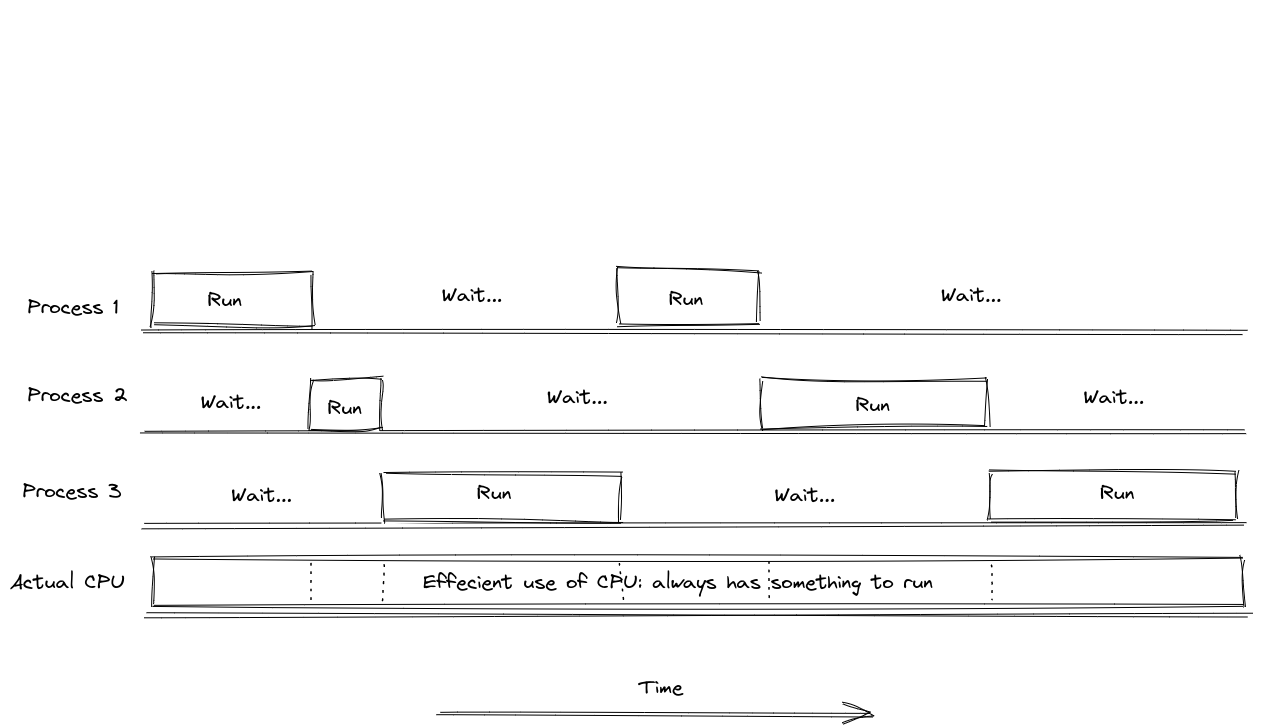
\includegraphics[width=350pt]{chapters/part-1/figures/processflow.png}
	\caption{A demonstration of running multiple processes on a single-core CPU.} \label{ch:pm:fig:processflow}
\end{figure}

The status of a process is stored in its \mync{Process Control Block}[PCB]. The PCB is a special data structure used to describe the metadata and the dynamic of a process. The OS manages the PCBs and control the processes accordingly. Some of the attributes of a PCB are summarized in Table \ref{ch:pm:tab:pcbcontent}.

\begin{table}[!htb]
	\centering \caption{Some attributes of a PCB.}\label{ch:pm:tab:pcbcontent}
	\begin{tabularx}{\textwidth}{lX}
		\hline
		Name & Description \\ \hline
		Process ID & The unique ID of the process.  \\
		State & The state of the process, for example, running, suspended, terminated.  \\
		Priority & Priority level in comparison with other processes. \\
		Program Counter & A pointer to the next line of program to be executed. \\
		Memory regions & A pointer to the RAM where the code and data of the process is stored. \\
		Accounting Information & Time limits, clock time used, etc. \\ \hline
	\end{tabularx}
\end{table}

A process shall at least have the following states. The fundamental states of a process and their transferring are introduced in Fig \ref{ch:pm:fig:processstatetransfer}, where ``blocked'' indicates that the process is waiting for other inputs to carry out the remaining part of the program, and ``suspended'' indicates that the process is hold for some reasons. When a process is offloaded from the CPU, its context is moved from the CPU registers to the PCB of the progress.

\begin{figure}[!htb]
	\centering
	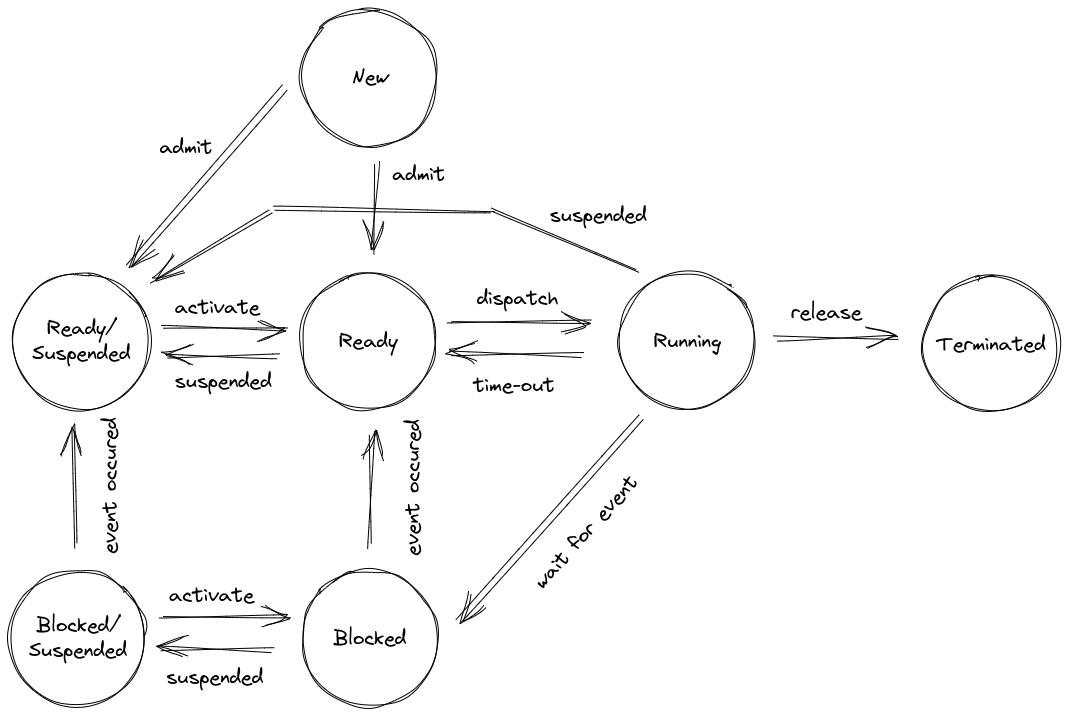
\includegraphics[width=350pt]{chapters/part-1/figures/processstatetransfer.png}
	\caption{Fundamental states of a process and their transferring.} \label{ch:pm:fig:processstatetransfer}
\end{figure}

There are different types of processes. For example, based on the source of the processes, there are OS triggered processes and user triggered processes, the first of which usually has a higher priority. Based on the running environment, there are front-ground processes and background processes. Based on the resources used, there are CPU processes and I/O processes.

A process usually has a relatively isolated environment, and it does not share memory storage with other processes. Special inter process communication mechanism, which is often referred as ``pipe'', is required for processes to talk to each other. Inter process communication requires OS level controls.

\subsection{Thread}

A \mync{thread} is like a work dispatch inside a process. There can be multiple threads in a process, as shown in Fig \ref{ch:pm:fig:threadinprocess}. Each thread has its own CPU register values and stack, but they share the same program, memory and file storage addresses.
\begin{figure}[!htb]
	\centering
	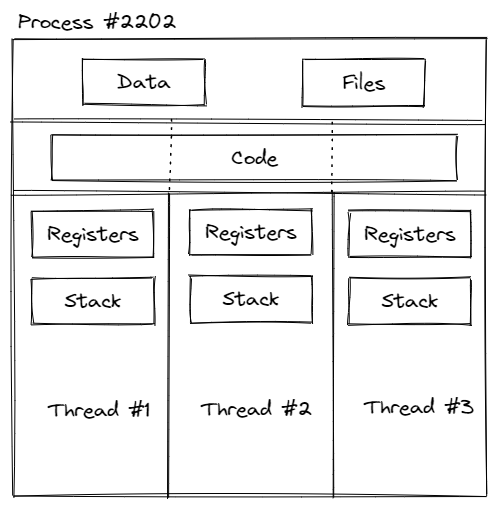
\includegraphics[width=200pt]{chapters/part-1/figures/threadinprocess.png}
	\caption{A demonstration of multiple threads in a process.} \label{ch:pm:fig:threadinprocess}
\end{figure}

Threads differ from processes in the following aspects:
\begin{itemize}
  \item A thread is lighter than a process, occupying less resources to create.
  \item Sharing memories and resources among threads in a process is easier than sharing among processes, because they naturally share address space.
  \item It is easier to enable parallel computation for the threads in the process when it is running on a multi-core CPU.
\end{itemize}

Notice that for many OS, including Linux, the kernel can provide thread level services.

\section{Process Management in Linux}

Basic process management commands including monitoring and terminating a process are given. Switching a process between foreground and background is also introduced.

\subsection{Monitor Process}

Two commands, \verb|ps| and \verb|top|, are widely used in monitoring the running process in the OS. They can be used stand-alone, without additional arguments as follows.
\begin{lstlisting}
$ ps [options]
\end{lstlisting}
or
\begin{lstlisting}
$ top
\end{lstlisting}

The major difference between these two commands is that \verb|ps| provides a snapshot (in a text format) of a list of processes, each with its name, \myabb{Process ID}{PID} and owner, etc., while \verb|top| provides a dynamic and frequently refreshing display of the running processes as well as their associated resources usage. Figs \ref{ch:pm:fig:pscommand} and \ref{ch:pm:fig:topcommand} give a quick demo of how the execution of the two commands look like.

\begin{figure}[!htb]
	\centering
	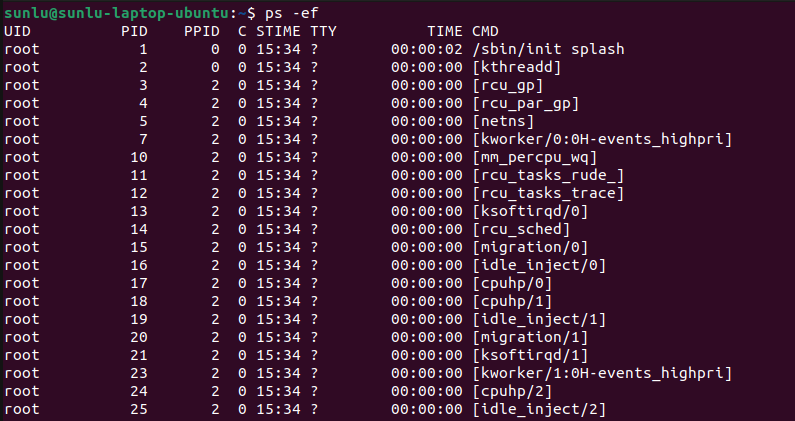
\includegraphics[width=300pt]{chapters/part-1/figures/pscommand.png}
	\caption{Execution of \texttt{ps -ef} command.} \label{ch:pm:fig:pscommand}
\end{figure}

\begin{figure}[!htb]
	\centering
	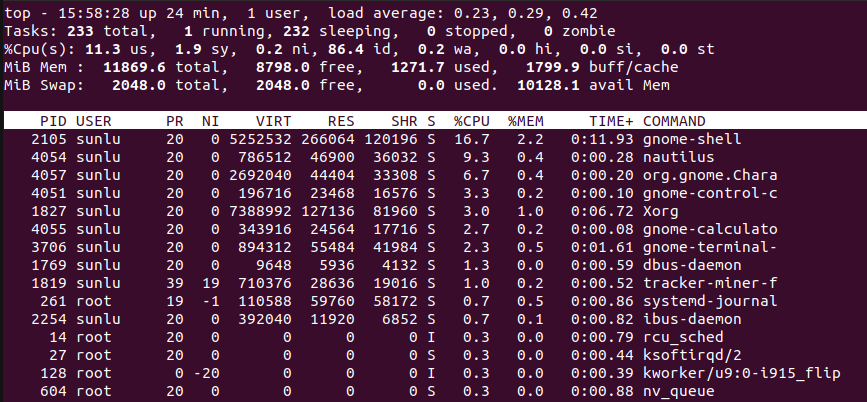
\includegraphics[width=300pt]{chapters/part-1/figures/topcommand.png}
	\caption{Execution of \texttt{top} command.} \label{ch:pm:fig:topcommand}
\end{figure}

Notice that \verb|top| is a running application where the user can keep interacting with to filter for particular processes, while \verb|ps| is more of a one-time command and its output can be saved into a text file for further processing.

Some commonly used options for \verb|ps| are summarized below.
\begin{itemize}
	\item \verb|-e|: list all processes
	\item \verb|-f|: list details of the processes
	\item \verb|-C <command name>| filter by command
	\item \verb|-u <username>| filter by user
\end{itemize}

\subsection{Terminate a Process}

To kill a process, use the \verb|kill| command as follows.
\begin{lstlisting}
$ kill <option> <process ID>
\end{lstlisting}

The \verb|kill| command offers different options to kill a process. Use \verb|kill -l| to list down the options as given below (and many more).
\begin{lstlisting}
1) SIGHUP    2) SIGINT    3) SIGQUIT   4) SIGILL
5) SIGTRAP   6) SIGABRT   7) SIGBUS    8) SIGFPE
9) SIGKILL  10) SIGUSR1  11) SIGSEGV  12) SIGUSR2
13) SIGPIPE 14) SIGALRM	 15) SIGTERM  16) SIGSTKFLT
17) SIGCHLD 18) SIGCONT	 19) SIGSTOP  20) SIGTSTP
...
\end{lstlisting}

Commonly used \verb|kill| options are \verb|kill -9| (SIGKILL) and \verb|kill -15| (SIGTERM) followed by the PID. It is mostly recommended to use \verb|kill -15| over \verb|kill -9|, as it allows the process to clean up and terminate properly. Most well designed software defines the protocol to terminate the process in a safe way. This is also the default termination option. Command \verb|kill -9|, on the other hand, force the OS to terminate the process immediately. It is used mostly when the process is not responding and cannot be terminated using \verb|kill -15|.

Another command \verb|killall| runs similarly as \verb|kill|, except that it kills signals based on the command, not the process ID. As a result, it is possible to use it to kill multiple signals with the same command at a time. Use it with cautions.

Notice that in Linux the process is arranged in a tree structure; killing a parent process will automatically terminate its children processes, and killing a child process may result in its parent process to restart a new child process.

\subsection{Switch between Foreground and Background}

To start a command as a background process, use \verb|&| in the end of the command as follows
\begin{lstlisting}
$ <command> &
\end{lstlisting}
This is useful if a command is time consuming and it does not need additional user interaction while running.

To check commands running in the background, use
\begin{lstlisting}
$ jobs
[1] <status> <command>
[2] <status> <command>
[3]+ <status> <command>
[4]- <status> <command>
...
\end{lstlisting}
A plus sign ``\verb|+|'' indicates that the command was the most recent one placed in the background, and the minus sign ``\verb|-|'', the second most recent one. To bring a background command to the foreground, use
\begin{lstlisting}
$ fg %<job number>
\end{lstlisting}
where \verb|<job number>| is the index given in \verb|jobs| outputs. If no job number is given, the most recent job will be brought to the foreground.

\subsection{Change Process Priority}

The priority of a process is given by an integer between $-100$ and $39$, the smaller the more prioritized. This value can be viewed using \verb|top|, as shown in Fig. \ref{ch:pm:fig:topcommand} under column ``PR''. The process with priority $-100$ is displayed as \verb|rt|, indicating the highest priority.

The entire priority range from $-100$ to $39$ is divided into two portions. The priority between $-100$ and $-1$ is known as ``real-time'', and between $0$ and $39$, ``normal''. In practice, real-time processes are mainly managed by the root user and are not accessible to regular users. A regular user's process typically falls within the normal priority range of $0$ to $39$. 

A ``\mync{NICE value}'' is assigned to the priorities. The priority $0$ corresponds with NICE value of $-20$, and $39$ with $19$. The user can adjust the NICE value of his process and hence change its priority. This is demonstrated by Fig. \ref{ch:pm:fig:priority}.

\begin{figure}[htbp]
	\centering
	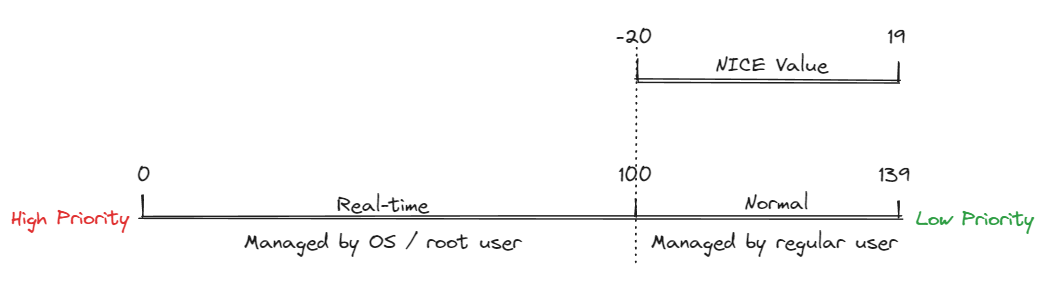
\includegraphics[width=300pt]{chapters/part-1/figures/priority.png}
	\caption{Priority levels in Linux.} \label{ch:pm:fig:priority}
\end{figure}

For normal processes, their NICE values can be viewed using \verb|top| as shown in Fig. \ref{ch:pm:fig:topcommand} under column ``NI''. Real-time processes do not use NICE value, hence NI are displayed as $0$ for these processes.

A properly designed OS should have built-in algorithms to manage process priorities and scheduling. However, tools like \verb|nice| and \verb|renice| are provided to give users and administrators the ability to influence these priorities in specific situations. Examples are given below.

To start a command with a specified NICE value, use
\begin{lstlisting}
$ nice -n <increment> <command>
\end{lstlisting}
and \verb|<increment>| will be the NICE value of the command.

To change the NICE value of an existing process, use
\begin{lstlisting}
$ renice -n <increment> -p <prosess id>
\end{lstlisting}
where \verb|<increment>|, being either positive or negative, will be added to the current NICE value of the process with the specified process ID.

It is also possible to manage the priorities not by individual process ID, but by a group of processes. This is useful when a group of processes belongs to a similar service or to a group of users, and we want to change the priority of the service or users all together.
















\part{Linux Advanced}
%\chapterauthor{Author Name}{Author Affiliation}
%\chapterauthor{Second Author}{Second Author Affiliation}
\chapter{Administration} \label{ch:administration}
...

\section{Introduction to Linux Administration}
...


\section{Root Account Management}

Managing and protecting the root user account is a key portion in Linux administration. It is worth mentioning that the root user is different from a sudoer, i.e., a user that can use \verb|sudo| command, although they both have elevated privileges when comes to system administration. A more detailed explanation is given below.

The root user refers to the user that is created by the system upon first installation of the OS. Its username is by default ``root'', with a UID of 0, and a GID of 0. Its home directory is by default \verb|/root| instead of \verb|/home/<user name>|. The default prompt for the root user is often \verb|#| instead of \verb|$| for other users. The root user has administrative privileges and can do almost anything without being denied or questioned by the system. As a commonly used safety practice, the password for the root user is usually disabled, thus nobody can login to the system as the root user using username and password authentication.

Notice that in theory the root user does not necessarily need to use the username ``root'', although it is a default convention. The administrative  comes with the UID of 0, not the username. Thus, it is possible to assign the administrative account a different username. It is also possible to create multiple accounts with administrative privileges by assigning UID of 0 to multiple accounts, although it is not recommended to share the same UID among different users.

Although the administrative privilege of root user does not come with its username, in some systems, the username ``root'' is given elevated privilege anyway. More details about this is introduced later.

Check the root user information as follows.
\begin{lstlisting}
$ cat /etc/passwd | grep ^root
root:x:0:0:root:/root:/bin/bash
\end{lstlisting}
where the third and fourth column of above give the UID and GID of the root user, respectively.

For comparison, a regular user would have far different UID and GID as shown below.
\begin{lstlisting}
$ cat /etc/passwd | grep ^sunlu
sunlu:x:1000:1000:Sun Lu,,,:/home/sunlu:/bin/bash
\end{lstlisting}

A sudoer refers to the regular users who can temporarily elevate its privileges and execute administration commands using \verb|sudo <privileged-command>|. A sudoer can also switch to root user prompt using \verb|sudo su| (and quit root user prompt using \verb|exit|). Their sudo privilege comes from the fact that they are included in the ``sudo group''.

Use \verb|groups| to check existing defined groups in the system, and \verb|groups <user name>| the groups a user is engaged. An example is given below.
\begin{lstlisting}
$ groups
sunlu adm cdrom sudo dip plugdev lpadmin lxd sambashare docker
$ groups sunlu
sunlu : sunlu adm cdrom sudo dip plugdev lpadmin lxd sambashare docker
\end{lstlisting}

The elevated privilege of the sudoer group is defined in \verb|/etc/sudoers|. A section of the file is given below, where \verb|%| appeared in front of \verb|admin| and \verb|sudo| is used to indicate group name.
\begin{lstlisting}
# User privilege specification
root	ALL=(ALL:ALL) ALL

# Members of the admin group may gain root privileges
%admin ALL=(ALL) ALL

# Allow members of group sudo to execute any command
%sudo	ALL=(ALL:ALL) ALL
\end{lstlisting}

It is possible to give the root account a password, thus enabling root authentication. This approach is sometimes used for troubleshooting and recovering purposes, but it is not a good practice in routine operations.

\section{User Management}

xxx

















%\chapterauthor{Author Name}{Author Affiliation}
%\chapterauthor{Second Author}{Second Author Affiliation}
\chapter{Storage Management}

Upon installation of the system, the OS shall scan the machine, look for hard drives, and either automatically or manually partition it into partitions and mount the partitions to different locations in the OS such as \verb|/| (root directory), \verb|/home/|, swap space, etc.

It is often not necessary for a casual user to manage the partitions and mountings by himself as there is the option to let Linux installation handle them automatically. However, when comes to Linux servers where hardware and storage is scaled up and down frequently, it is recommended that the administrator shall understand how hard drive can be managed. Linux provides flexible tools to monitor and manage the storage of the machine, including manipulating partition table, format partition, and managing its mounting point.

\section{Partitions and Filesystems}

A partition is a logical slice of the hard drive managed by the OS via partition table which is introduced in more details in a later stage. A filesystem, on the other hand, reflects how OS formats data in the partition and where it is mounted in the OS filesystem hierarchy. This is demonstrated by Fig. \ref{ch:dm:fig:partition}.

\begin{figure}[htbp]
	\centering
	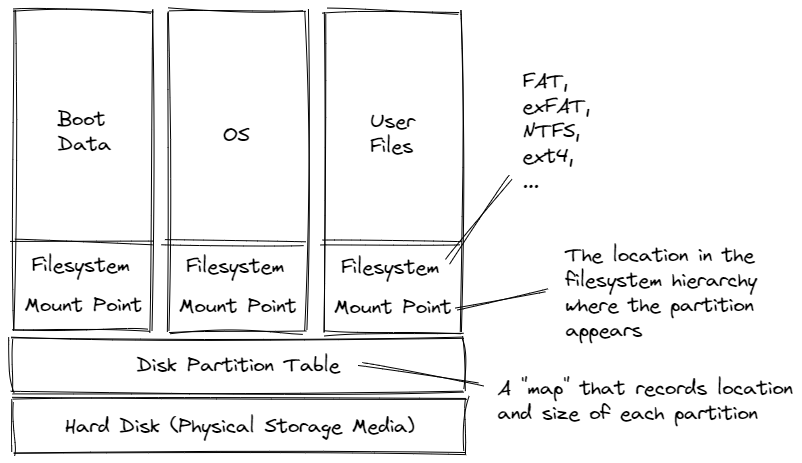
\includegraphics[width=300pt]{chapters/part-2/figures/partition.png}
	\caption{A demonstration of how a hard drive is used in the OS.} \label{ch:dm:fig:partition}
\end{figure}

Usually, each filesystem is associated with a partition. The partition focuses more on the logical separation of the hard drive, while the filesystem focuses more on how the operating system manages the data within that partition. Ideally they are consistent and there should be a clear correspondence. However, it is possible that when the filesystem is not sized correctly, the filesystem is smaller than its associated partition, and a part of the storage becomes unused. A filesystem is only meaningful on a partition because it describes how that partition is formatted and managed. Therefore, a filesystem cannot exist without a partition. However, a partition can exist without a filesystem. It will be an unused storage space that is not useful to the operating system until it is formatted with a filesystem.

A demonstration of partitions versus filesystems is given in Fig. \ref{ch:dm:fig:partitionvsfilesystem}.

\begin{figure}[htbp]
	\centering
	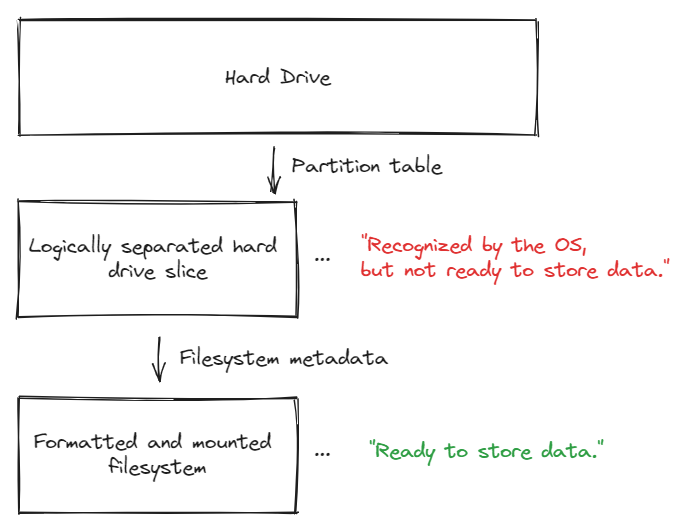
\includegraphics[width=300pt]{chapters/part-2/figures/partitionvsfilesystem.png}
	\caption{A demonstration of how partitions and filesystems relate to each other.} \label{ch:dm:fig:partitionvsfilesystem}
\end{figure}


Use \verb|df| to monitor the status of the mounted storage, including the filesystem name, size, and used percentage. Command \verb|df -h| gives a nice snapshot of the storage usage in a human-readable format. An example is given below.
\begin{lstlisting}
$ df -h
Filesystem      Size  Used Avail Use% Mounted on
tmpfs           1.2G  2.1M  1.2G   1% /run
/dev/sda3       916G   51G  818G   6% /
tmpfs           5.8G     0  5.8G   0% /dev/shm
tmpfs           5.0M  4.0K  5.0M   1% /run/lock
/dev/sda2       512M  5.3M  507M   2% /boot/efi
tmpfs           1.2G  120K  1.2G   1% /run/user/1000
\end{lstlisting}
from where it can be seen that the most of the storage of the system, in this case $818G$, is mounted on the root directory.

Use \verb|lsblk| to list information about block devices in the OS. Block devices refer to nonvolatile mass storage devices whose information can be accessed in any order, such as hard disks and CD-ROMs. An example is given below.
\begin{lstlisting}
$ lsblk
NAME   MAJ:MIN RM   SIZE RO TYPE MOUNTPOINTS
loop0    7:0    0     4K  1 loop /snap/bare/5
loop1    7:1    0    62M  1 loop /snap/core20/1593
loop2    7:2    0    62M  1 loop /snap/core20/1611
loop3    7:3    0 163.3M  1 loop /snap/firefox/1670
loop4    7:4    0   177M  1 loop /snap/firefox/1749
loop5    7:5    0 400.8M  1 loop /snap/gnome-3-38-2004/112
loop6    7:6    0 248.8M  1 loop /snap/gnome-3-38-2004/99
loop7    7:7    0  81.3M  1 loop /snap/gtk-common-themes/1534
loop8    7:8    0  91.7M  1 loop /snap/gtk-common-themes/1535
loop9    7:9    0  45.9M  1 loop /snap/snap-store/575
loop10   7:10   0    47M  1 loop /snap/snapd/16010
loop11   7:11   0  45.9M  1 loop /snap/snap-store/582
loop12   7:12   0    47M  1 loop /snap/snapd/16292
loop13   7:13   0   284K  1 loop /snap/snapd-desktop-integration/10
loop14   7:14   0   284K  1 loop /snap/snapd-desktop-integration/14
sda      8:0    0 931.5G  0 disk
|-sda1   8:1    0     1M  0 part
|-sda2   8:2    0   513M  0 part /boot/efi
|-sda3   8:3    0   931G  0 part /
sr0     11:0    1  1024M  0 rom
\end{lstlisting}
which gives the size, the type and the mount point of all the storages.

Use \verb|blkid| to print block device attributes. An example is given below.
\begin{lstlisting}
$ blkid
/dev/sda3: UUID="d0b15b7c-71f2-41f4-b67a-e7c69446feab" BLOCK_SIZE="4096" TYPE="ext4" PARTUUID="4b570507-6aa0-46c7-ac1b-06cb4c8bdb61"
\end{lstlisting}

\section{Disk Partition Table Manipulation}

Due to the development of computer science and OS, manual disk partition is less necessary than before for a casual user. Nevertheless, Linux provides necessary tools for disk partition table manipulation and they are introduced in this section.

\subsection{Disk Partition}

Disk partitioning refers to the action of creating one or more regions on secondary storage (e.g., disk) so that they can be managed separately, as if they are different ``virtual disks''. An example of disk partitioning on a Windows PC would be to partition a $1TB$ hard drive into $512GB$ of \verb|C:\| drive and $512GB$ of \verb|D:\| drive. Partitioned regions are logically separated. The partitions locations and sizes are stored in the disk partition table.

Some of the reasons for using disk partition include:
\begin{itemize}
  \item Due to capability limitation, OS cannot handle a very large disk storage as a whole (this is less the case nowadays).
  \item Different types of files, for example system data and user data, can be stored separately for easy management.
  \item Different filesystems can be used on different partitions.
  \item Different partitions can be configured differently with unique settings.
  \item Sometimes partitioning can speed up hard disk accessing.
\end{itemize}

\subsection{Disk Partition Table Manipulation}

From the output of \verb|lsblk| command earlier, it is clear that the system's hard disk name is ``\verb|sda|''. To get a bit more details on this disk and its current partitioning status, use
\begin{lstlisting}
$ sudo fdisk -l | grep sda
Disk /dev/sda: 931.51 GiB, 1000204886016 bytes, 1953525168 sectors
/dev/sda1     2048       4095       2048    1M BIOS boot
/dev/sda2     4096    1054719    1050624  513M EFI System
/dev/sda3  1054720 1953523711 1952468992  931G Linux filesystem
\end{lstlisting}

From the above result, it can be seen that the disk registered under \verb|/dev/| (this is where the devices are represented by default) has been partitioned into 3 partitions, and the user space that can be further modified is \verb|/dev/sda3| which is $931GB$.

There are variety of tools that can be used for disk partitioning. A common way of doing that is to use
\begin{lstlisting}
$ sudo fdisk /dev/sda3
\end{lstlisting}
to enter the fdisk utility, and follow the wizard.

Other tools such as \verb|cfdisk| and \verb|parted| can also be used similarly for disk partition.

\section{Mount, Unmount and Format a Partition}

The hard disk can be formatted by partition, from where a new filesystem can be created. To format a partition, double check using \verb|lsblk| to make sure that it is not mounted in the system. Use \verb|sudo umount <partition name>| to unmount a partition.

Use \verb|sudo mkfs| to format and create a new formatted filesystem, then use \verb|mount| to mount it back to the OS. The mount of a partition needs to be recorded into \verb|/etc/fstab| so that the OS would remember it after a reboot.

\chapter{Service Control}
...
\section{Service Control} \label{ch:sa:sec:sc}

There are many services running in the background of the OS, some of which started by the OS while the other by the user. For example, Apache service might be used when the system is hosting a webpage. Other commonly used services include keyboard related services, bluetooth services, etc.

To quickly have a glance of the running services, use
\begin{lstlisting}
$ systemctl --type=service
\end{lstlisting}

These services can be managed using service managing utilities such as \verb|systemctl| and \verb|service|. Some commonly used terminologies are concluded in Table \ref{ch:sa:tab:servicecontroltools} with explanations about their differences.

\begin{table}
	\centering \caption{Commonly seen terminologies regarding service control.}\label{ch:sa:tab:servicecontroltools}
	\begin{tabularx}{\textwidth}{lX}
		\hline
		Term / Tool name & Description \\ \hline
		\verb|systemd| & The \verb|systemd|, i.e., \textit{system daemon}, is a suite of basic building blocks for a Linux system that provides a system and service manager that runs as PID 1 and starts the rest of the system.  \\ \hdashline
		\verb|systemctl| & The \verb|systemctl| command interacts with the \verb|systemd| service manager to manage the services. Contrary to \verb|service| command, it manages the services by interacting with the \verb|Systemd| process instead of running the init script.  \\ \hdashline
		\verb|service| & The \verb|service| command runs a pre-defined wrapper script that allows system administrators to start, stop, and check the status of services. It is a wrapper for \verb|/etc/init.d| scripts, Upstart's \verb|initctl| command, and also \verb|systemctl|. \\ \hline
	\end{tabularx}
\end{table}

In short, \verb|systemd| is the back-end service of Linux that manages the services. Both \verb|systemctl| and \verb|service| are tools to interact with \verb|systemd| (and other back-end services) to manage the services. Generally speaking, \verb|systemctl| is more straightforward, powerful and more complicated to use, while \verb|service| is usually simpler and user-friendly.

Use the following commands to check the status of a service, and start, stop or reboot the service.
\begin{lstlisting}
$ sudo systemctl status <service name>
$ sudo systemctl start <service name>
$ sudo systemctl stop <service name>
$ sudo systemctl restart <service name>
\end{lstlisting}

Use the following commands to enable and disable a service. An enabled service automatically starts during the system boot, and a disabled service does not.
\begin{lstlisting}
$ sudo systemctl enable <service name>
$ sudo systemctl disable <service name>
\end{lstlisting}

Use the following command to mask and unmask a service. A masked service cannot be started even using \verb|systemctl start|.
\begin{lstlisting}
$ sudo systemctl mask <service name>
$ sudo systemctl unmask <service name>
\end{lstlisting}

The \verb|service| command can be used in a similar manner as follows.
\begin{lstlisting}
$ sudo service <service name> status
$ sudo service <service name> start
$ sudo service <service name> stop
$ sudo service <service name> restart
\end{lstlisting}


\part{Widely Used Services}
\chapter{Git}

\mync{Git} is a distributed version-control system for tracking changes during the software development, and it can be used on cross platforms including Windows, Unix/Linux and MacOS. 

This chapter introduces the basic use of Git on a local Linux machine and with a remote repository host server such as GitHub. \mync{Continuous Integration and Continuous Deployment}[CI/CD], an important concept in nowadays software development and operation, is also briefly covered. For CI/CD, \mync{GitHub Action} is introduced.

\section{Introduction}

Git, created by Linus Trovalds in 2005, is a distributed version-control system for tracking changes in source code and files. It is helpful with maintaining data integrity during the collaborative development of a software in distributed non-linear work flows. Git is free and open-source software under GNU general public license.

With Git, all computers participating in the software development store a copy of the full-fledged repository locally with complete history, and it can synchronize with a centralized remote server. It introduces the concept of ``\mync{branch}'', to be more precise ``master'' and ``slave'' branches to manage the concurrent development of different features of the project, where the master branch is the stable and shared repository among everyone, and the slave branches are copies of the master branch where individual features can be developed. For a slave branch, once its developed feature is approved, it can be merged back to the master branch. A demonstration is given in Fig. \ref{ch:sma:fig:gitflow}.
\begin{figure}[htbp]
	\centering
	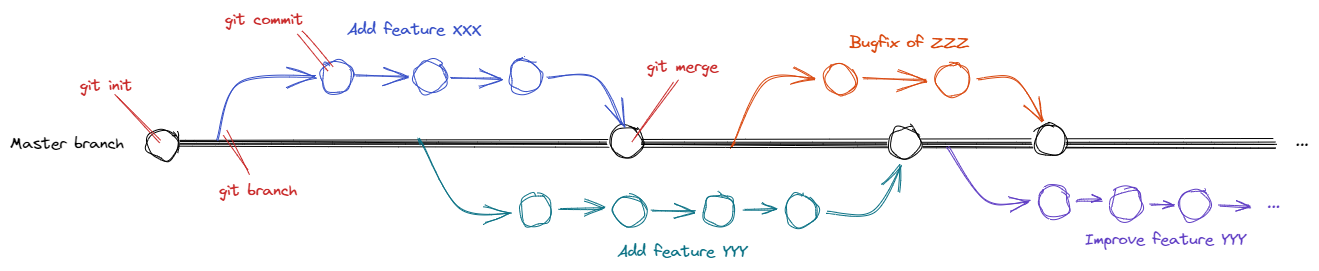
\includegraphics[width=350pt]{chapters/part-3/figures/gitflow.png}
	\caption{Git for software development management.} \label{ch:sma:fig:gitflow}
\end{figure}

CLI is often used to manage a Git repository. Some commonly used commands are shown in Fig. \ref{ch:sma:fig:gitflow} and more to be introduced later. Notice that a graphical user interface is also available to interact with \verb|git|. However, in the scope of this notebook, command line is mostly used.

\section{Setup}

To use Git, follow the instructions to install and configure the software.

\subsection{Installation}

Git and its relevant documents can be obtained from its official website \textit{https://git-scm.com/}. In many Linux distributions, Git is pre-installed. If Git is missing in the machine, follow the instructions on the official website to install it on the computer. Notice that the installation procedure may differ with different OS.

\subsection{Configuration}

Upon successful installation, it is recommended to use \verb|git config| for some basic configurations. Notice that there are two types of configurations, namely the global configurations (apply to the machine and the user), and the repository configurations (apply to a particular Git repository). By default, the global level configurations are stored under \verb|~/.gitconfig| and the repository level configurations \verb|./.git/config| in the repository. A good practice to edit these configurations is to use Git commands rather than editing the files directly.

To add user name and email to the global configuration, use
\begin{lstlisting}
$ git config --global user.name '<user name>'
$ git config --global user.email '<user email>'
\end{lstlisting}
To retrieve the global configuration, use
\begin{lstlisting}
$ git config --global -l
\end{lstlisting}
To revoke a global configuration, use
\begin{lstlisting}
$ git config --global --unset <configuration>
\end{lstlisting}
For example,
\begin{lstlisting}
$ git config --global --unset user.name
\end{lstlisting}
removes the user name.

More details about \verb|git config| can be found at \textit{https://git-scm.com/docs/git-config}. Usually, the user name and email configurations are mandatory, as they are very useful information in developing collaborative projects.

\section{Local Repository Management}

A \mync{Git repository} refers to the ``ecosystem'' Git uses to manage a project. To be more specific, it refers to the \verb|.git| file associated with each Git-managed project, using which Git tracse the development of the project. 

Git manages the repositories locally, and it can also synchronize them with remote upstreams if they have one. This section considers local repository management.

\subsection{Initialization of a Repository}

Navigate to the project directory. Use the following command to create a new Git repository for the project.
\begin{lstlisting}
$ git init
\end{lstlisting}
From this point forward, Git monitors everything that happens inside this directory and its subdirectories and tries to track any change to the files, unless otherwise configured specifically. Many Git-relavent CLI commands, for example \verb|git status| to check the status of the repository, become available. More details are introduced later.

\subsection{Version Tracking}

For simplicity, assume that there is only one branch in the repository, namely the master branch. Notice that when there are multiple branches, the version-tracking works the same for each and every branch in a separate and independent manner.

The mechanism behind version tracking is briefly introduced as follows. This helps the user to better understand how Git works and how the CLI commands are designed.

The project directory is split into two parts, outside \verb|./.git/| the workspace, and inside \verb|./.git/| the Git repository. The workspace has the up-to-date project contents and it is directly managed by the user, while Git repository is managed by Git. The user should not manage the repository directly unless using the Git interface.

Inside the Git repository are metadata of the workspace files such as which files have been changed since the last deployment, etc. It also stores a full back up of every historical versions of the project (with powerful compressing mechanisms, of course). It is worth mentioning that instead of recording the changes of a file from version to version, Git records the snapshot of the file in every version, unless it is left untouched between two consecutive versions.

Figure \ref{ch:sma:fig:gitbasics} gives a demonstration of how Git manages the project directory. Git classifies files in the workspace into different status, as shown in Fig. \ref{ch:sma:fig:gitbasics}. A brief explanation of each types is given in Table \ref{ch:sma:tab:gitbasics}. Detail explanations of ``stage'' and ``commit'' are given later.
\begin{figure}[!htb]
	\centering
	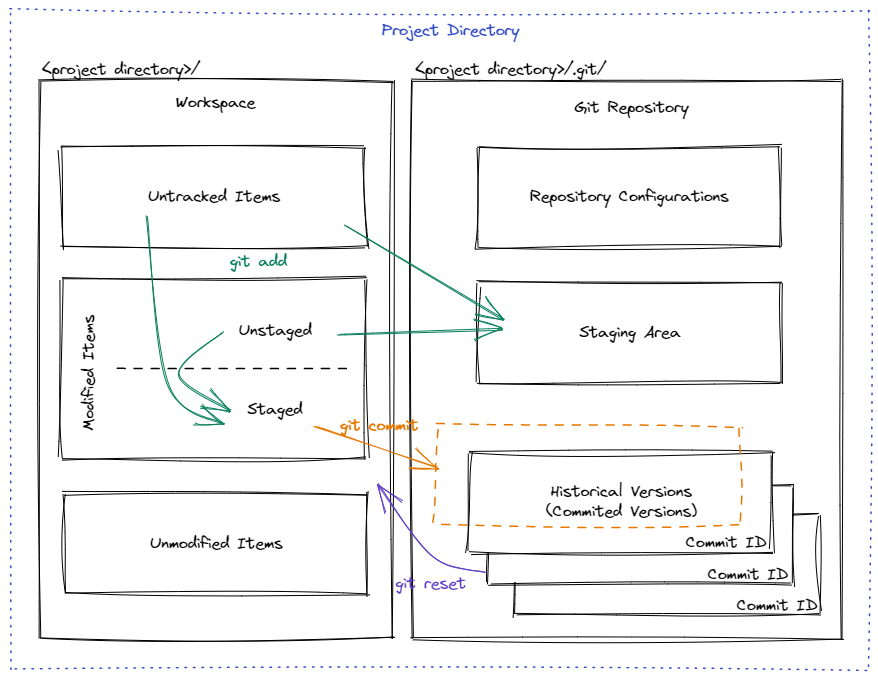
\includegraphics[width=350pt]{chapters/part-3/figures/gitbasics.png}
	\caption{The project directory managed by Git.} \label{ch:sma:fig:gitbasics}
\end{figure}

\begin{table}
	\centering \caption{Different file status in a Git managed project.}\label{ch:sma:tab:gitbasics}
	\begin{tabularx}{\textwidth}{lX}
		\hline
		Status & Description \\ \hline
		Untracked & Newly added or renamed items in the project directory.  \\ 
		Modified (Unstaged) & Modified items from the last version that has not been registered in the staged area.  \\ 
		Modified (Staged) & Modified items from the last version that has been registered in the staged area. Notice that an untracked item can be staged directly, skipping ``modified (unstaged)'' step. Use \verb|git add| to stage items. \\ 
		Unmodified & Unmodified items from the last version. Use \verb|git commit| to update a new version, which would change all the staged items into unmodified items. \\ \hline
	\end{tabularx}
\end{table}

Use \verb|git status| to check the file status in the project. An example is given below.
\begin{lstlisting}
$ git status
On branch master

Changes to be committed:
  (use "git restore --staged <file>..." to unstage)
	modified:   chapters/ch-software-management-advanced/ch.tex

Changes not staged for commit:
  (use "git add <file>..." to update what will be committed)
  (use "git restore <file>..." to discard changes in working directory)
	modified:   appendix/ap.tex
	modified:   main.pdf

Untracked files:
  (use "git add <file>..." to include in what will be committed)
	chapters/ch-software-management-advanced/figures/
\end{lstlisting}
where \verb|ch.tex| is a modified (staged) item; \verb|ap.tex| and \verb|main.pdf| modified (unstaged) items, and \verb|figures/| an untracked item.

It takes a two-step procedure to back up the project in the Git repository. In the first step, the user flags the changed items (either newly added, renamed, or modified) to be backed up in the next version. In the second step, the user actually backs up the items. The first and second steps are called ``stage'' and ``commit'' respectively. Notice that it is possible to run a single line of command to execute both steps, but logically it still takes two steps.

Git tracks the name and content of the items that the user has staged in the ``staging area'' as shown in Fig. \ref{ch:sma:fig:gitbasics}. Think of staging items as taking a snapshot of the items. However, the snapshot at this stage is temporary and has not been backed up in the repository yet. The actual backup happens later when the staged items are committed. To stage an item, use
\begin{lstlisting}
$ git add <item name>
\end{lstlisting}
which registers the item in the staging area, thus also changes its status from untracked or modified (unstaged) to modified (staged). If an item is modified after it has been staged, Git will distinguish the ``staged portion'' and ``unstaged portion'' of that item. If using \verb|git status| to check its status, the item will be listed as both staged and unstaged. Unstaged items, either untracked or modified, will remain its status after the commit. Sometimes for convenience, \verb|git add -A| can be used to add all untracked or modified items to the staging area.

Use \verb|git commit| to commit the staged items and back them up in the repository as follows.
\begin{lstlisting}
$ git commit [<item name>]
\end{lstlisting}
The above command commits the project and creates a version in the Git repository. It is possible to specify items, in which case Git only commits the specified items and leave the rest items as they are. A commit ID is automatically assigned to the commit. Notice that the user will be asked to provide a ``comment message'' with the commit, which should be used to briefly explain what has been changed in this commit.

A flag \verb|-a| with \verb|git commit| stages all changes made to the project, then implements the commit command. A flag \verb|-m| simplifies the message recording process and allows the user to key in the message directly after the command. An example is given below.
\begin{lstlisting}
$ git status
On branch master

Changes not staged for commit:
  (use "git add <file>..." to update what will be committed)
  (use "git restore <file>..." to discard changes in working directory)
        modified:   A Notebook on Linux/chapters/ch-software-management-advanced/ch.tex
        modified:   A Notebook on Linux/main.pdf

no changes added to commit (use "git add" and/or "git commit -a")

$ git commit -am "add introduction to git command"
[master e2e977e] add introduction to git command
 2 files changed, 5 insertions(+), 4 deletions(-)

$ git status
On branch master

nothing to commit, working tree clean
\end{lstlisting}

To check the commit logs, i.e., all historical commits including their associated timestamps, authors, commit IDs and comment messages, use \verb|git log| as shown in the example below. Notice that the commit logs can be very long. Only a few commits are given for illustration purpose.
\begin{lstlisting}
$ git log
commit e3475e673d8c2a087de6b4423188c51e80af3e5d (HEAD -> master)
Author: sunlu <sunlu.electric@gmail.com>
Date:   Wed Aug 31 15:16:52 2022 +0800

    git

commit 3ab6d1473a7e48d4d890509ddb5a87274c023e6c
Author: sunlu <sunlu.electric@gmail.com>
Date:   Tue Aug 30 15:50:06 2022 +0800

    k8s

commit f6a1e3d779305e966602ecd7589c05f56dd2ad0f
Author: sunlu <sunlu.electric@gmail.com>
Date:   Mon Aug 29 16:31:18 2022 +0800

    more on docker and kubernetes

commit e2de5b28db7982f57d0ad51361d5161b884f2efe
Author: sunlu <sunlu.electric@gmail.com>
Date:   Sun Aug 28 21:38:48 2022 +0800

    add docker sections
\end{lstlisting}
where notice that \verb|HEAD| is a reference that points to the latest commit in a branch. Filters can be added as optional arguments for the \verb|git log| command. More details are given at \textit{https://git-scm.com/docs/git-log}.

And finally, to restore to a previous commit version, use \verb|git reset| or \verb|git revert|. Notice that \verb|git reset| and \verb|git revert| can both be used to restore the workspace to a previous stage, but they differ significantly. In general, \verb|git reset| ``erases'' the past commits, and it is often used in the case where the changes and commits to be reset have not been uploaded to the upstream or shared distributively. Command \verb|git revert| on the other hand create a new commit that undoes all the changes, and it is often used when the changes and commits to revert are already distributed.

The command \verb|git reset| is often used as follows.
\begin{lstlisting}
$ git reset <option> <commit ID>
\end{lstlisting}
where \verb|<option>| is often \verb|--hard|, \verb|--mixed| or \verb|--soft|, and \verb|<commit ID>| can be the ID of any commit in the git log, or for shorcut \verb|HEAD| the latest commit, \verb|HEAD^| or \verb|HEAD~1| the second latest commit, \verb|HEAD~2| the third latest commit, and so on.

The options \verb|--hard|, \verb|--mixed| and \verb|--soft| work differently. All these options move \verb|HEAD| to the specified commit, and remove all commits afterwards from the repository. The \verb|--hard| option reverts the workspace back to when the specified commit happened (meaning that there would be no way to undo the reset command). Both \verb|--mixed| and \verb|--soft| do not change the workspace. The \verb|--mixed| option leaves all the changes from the specified commit to today as unstaged, while \verb|--soft| leaves them as staged. If no \verb|--hard|, \verb|--mixed| or \verb|--soft| is given, \verb|--mixed| will be used as the default option.

Notice that \verb|git reset| does not help if the unwilling changes and commits to be reverted have already been pushed and synchronized to a remote server or to other collaborators. This is because \verb|git reset| erases the history, and as a result \textit{git} would think that the reset repository is ``left behind'' when it synchronizes with other repositories. Consequently, it will simply synchronizes the changes and commits back.

In such cases, consider using \verb|git revert| instead. Syntax wise they work similarly. Instead of erase the history, \verb|git revert| creates a new commit whose content is copied and pasted from a past commit.

\subsection{Branch Management}

``Branch'' is one of the core features of Git, and it plays an important role in collaborative development of a project. There are two types of branches, namely the local branch and the remote branch. The remote branch is often the upstream mirror of the local branch used for sharing and synchronizing the project development with others. The details will be introduced in Section \ref{ch:sma:sec:rrm}. Only local branches are considered in this section.

To list down all the local branches, use
\begin{lstlisting}
$ git branch
\end{lstlisting}
and the current working branch will be highlighted. The current working branch is also referred as the ``head branch'' or the ``active branch''.

To create a new branch from the current branch, and to delete a branch, use
\begin{lstlisting}
$ git branch <new branch name> [<commit ID>]
$ git branch -d <branch name>
\end{lstlisting}
respectively. The optional \verb|<commit ID>| when creating a new branch allows the user to create a branch on top of a specified historical commit instead of the latest commit.

To rename a branch, use
\begin{lstlisting}
$ git branch -m [<old branch name>] <new branch name>
\end{lstlisting}
where if no \verb|<old branch name>| is specified, the current working branch will be renamed.

To switch to a different working branch, use \verb|git checkout| or \verb|git switch| as follows.
\begin{lstlisting}
$ git checkout <branch name>
$ git switch <branch name>
\end{lstlisting}
Notice that when there are uncommitted changes in the current branch, Git may forbid the user to switch to another branch (the rules are too complicated to be explained here). Therefore, it is recommended to commit the changes before switching to a different branch. When switching to another branch, the workspace will change accordingly to the target branch.

To merge a branch back to the current branch, use
\begin{lstlisting}
$ git merge <branch name>
\end{lstlisting}
and fill in the comments accordingly. For example, checkout to master branch, and use \verb|git merge <slave branch name>| to merge the features in the slave branch to the master branch. This often happens when the slave branch has finished developing and testing a new feature and is prepared to add the feature to the stable master branch. By default, Git automatically deletes the merged branch. This behavior can be changed in the configuration.

\begin{shortbox}
\Boxhead{Pull Request}

In a collaborative project, the master branch is managed very carefully because everything on that branch will affect the project deeply. There is often a group of senior developers who manage the master branch. Any code to be added to the master branch must be checked by one or a few of them.

When a slave branch wants the features developed on that branch to be merged to the master branch, the owner of the slave branch needs to raise a ``pull request''. As its name suggests, it requests the master branch to pull the updates from the slave branch. The master branch managers will then view and check the slave branch, making sure that everything is correct before they approve the merging.

\end{shortbox}

An alternative way of integrating two branches is \verb|git rebase|, which ``rewires'' the two branches into a linear single branch. Use \verb|git rebase| as follows.
\begin{lstlisting}
$ git rebase <branch name>
\end{lstlisting}
A demonstrative Fig. \ref{ch:sma:fig:gitrebase} explains the differences between \verb|git merge| and \verb|git rebase|. It is clear from Fig. \ref{ch:sma:fig:gitrebase} that by using \verb|git rebase|, all feature commits are integrated into the master repositories to form a single repository tracking line, which differs largely from \verb|git merge|.
\begin{figure}[htbp]
	\centering
	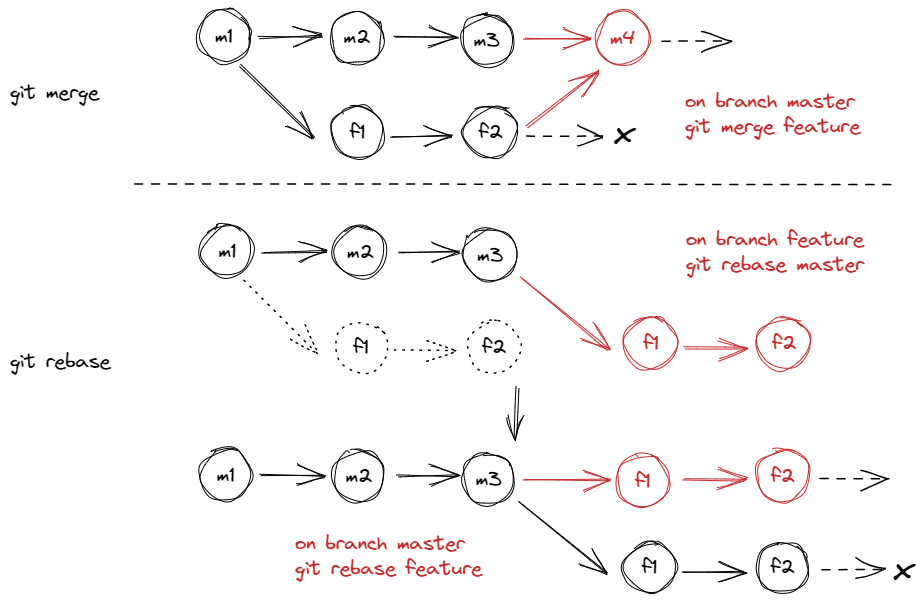
\includegraphics[width=350pt]{chapters/part-3/figures/gitrebase.png}
	\caption{Two approaches of integrating branches, \texttt{git merge} VS \texttt{git rebase}.} \label{ch:sma:fig:gitrebase}
\end{figure}

An intuitive way to understand \verb|git rebase| is given as follows. Imagine two branches $A$ and $B$ that have diverged from the same commit $O$. On branch $A$, execute \verb|git rebase B|. Here is a step-by-step breakdown of what happens:
\begin{enumerate}
	\item Identify common ancestor of the current branch $A$ and the rebase branch $B$, which is commit $O$ in this example.
	\item Back up commits happened on branch $A$ since commit $O$. Assume they are commits $A_1$, $A_2$, ..., $A_n$.
	\item Reset branch $A$ to Branch $B$ and $A$ now starts from the tip of $B$.
	\item Reapply commits $A_1$, $A_2$, ..., $A_n$ on the reset $A$ in a sequential manner, potentially leading to conflicts that need to be resolved manually.
\end{enumerate}
After the rebase operation, the history of branch $A$ appears as if it was developed sequentially from the end of branch $B$, effectively integrating the changes of $B$ into $A$ in a linear history.

\section{Remote Repository Management} \label{ch:sma:sec:rrm}

In collaborative projects, the repository and branches are stored and shared in one or more cloud servers. Each developer can interact with the repository on the cloud by pulling changes or pushing updates. The developer does not directly make changes to the repository or branches on the cloud. Instead, he clone the repository to his local machine and manipulate branches locally. The local repository and branches are then synchronized with the cloud repository and branches using Git commands. This is known as remote repository management and it is introduced in this section.

Depending on the cloud servers that host the remote repository, different services might be available. In the scope of this notebook, GitHub is considered as the remote repository host. GitHub is an internet hosting service for software development and sharing using Git. A user can create, manage, share and co-develop remote repositories on GitHub. Notice that GitHub is not the only place to host remote repositories. Some alternatives include \textit{GitLab} and \textit{Gitee}. Using Git, it is even possible to build a repository hosting server on premises using a regular computer. In this notebook, only GitHub is studied.

An \textit{https} URL is associated with each remote repository on GitHub, for example \textit{https://github.com/torvalds/linux.git} for Linux kernel. This URL can be used to download the remote repository to a local machine, or to link (synchronize) a local repository with that remote repository.

Consider the case where there is already a remote repository, either under the user's GitHub account or from the community. To download a clone of an existing repository to the local machine, use
\begin{lstlisting}
$ git clone <repository URL> [<local directory>]
\end{lstlisting}
and to maintain the local repository up-to-date with the remote repository, regularly use
\begin{lstlisting}
$ git remote update
$ git pull
\end{lstlisting}
to synchronize the local repository with the remote one.

\begin{shortbox}
\Boxhead{Should I use \texttt{git pull}?}

One may argue whether it is a good idea to use \verb|git pull|. Although convenient, \verb|git pull| is an integration of two commands, \verb|git fetch| and \verb|git merge| (or \verb|git rebase|) executed sequentially. It may be ``safer'' to manually run the two commands separately.
\end{shortbox}

The local commits can also be pushed to the remote repository using
\begin{lstlisting}
$ git push
\end{lstlisting}
if the remote repository is under the user's account, or if the owner of the remote repository gives the user the permission. Notice that when pushing updates to the remote repository, GitHub may require login credentials, for example username and password pair or SSH key, for permission checks.

Consider another case where there is already a well developed local repository. An empty remote repository has just been created on GitHub which is to be setup to mirror the local repository. To link the remote and local repositories, navigate to the local repository and use
\begin{lstlisting}
$ git remote add <remote repository name> <repository URL>
\end{lstlisting}
which will register the remote repository URL in the local configuration file. A commonly used remote repository name is ``origin''. The next step is to map the local current working branch with a branch in the remote repository, which would be used as the default source/target branch when running \verb|git pull| and \verb|git push|. This can be done as follows.
\begin{lstlisting}
$ git branch --set-upstream-to <remote repository name> <remote repository branch>
\end{lstlisting}
Notice that this step is not required if the project is cloned from a remote repository using \verb|git clone| introduced earlier, as it will automatically setup the upstream using the source of the clone.

From there on, use \verb|git push| and \verb|git pull| normally.

By assigning upstream branch to a local branch and \verb|git push| the local branch to the upstream, Git will update or create the remote branch accordingly. A remote branch can be deleted with a \verb|-d| flag while using \verb|git push|.

\section{\textit{GitHub Actions}}

\textit{GitHub Actions} is essentially a tool that allows the user to define a pipeline of actions when something changed in the GitHub remote repository, for example a pull request is raised, a new commit is pushed, etc. \textit{Actions} is useful as part of CI/CD. More details are given in Appendix \ref{ch:cicd}.
 
\chapter{Database}

Database and database manage systems (DBMS) are introduced in this and consecutive chapters. Both relational and non-relational databases are covered. Tools and languages to manipulate databases, such as structured query language (SQL) for relational databases, are introduced.

\section{Relational Database}

Database, in a broad view, refers to an organized collection of data of any format. In this sense, any file format that hosts information in a meaningful and explainable way, such as \textit{CSV}, \textit{XML} and \textit{JSON}, is a database. These file formats often work fine when the data is stored in a centralized manner and its size small.

As the data size grows, the robustness and efficiency of storing and retrieving data become challenging, and different database models have been proposed to tackle it. Dedicated software, namely DBMS, is developed to manage and maintain the database and provide an interface for the users to create, retrieve, update and delete data. Different database models require different database engines and DBMS, and different DBMS may provide different interfaces for the users.

There are many database models available in the market. The most widely seen database models can be divided into two categories, namely the relational databases (RDB) and the non-relational databases.

Relational database was proposed in 1970s by IBM. Some important features of a relational database include the following.
\begin{itemize}
	\item Structure the data as ``relations'', which is a collection of tables, each consisting of a set of rows (also known as tuple/record) and columns (also known as attribute/field).
	\item For each table, a primary key, either being a column or a combination of several columns, is defined that can uniquely distinguish a row from others.
	\item Provide relational operations that manipulate the data in the tables, for example, joining tables together and aligning them using an attribute.
\end{itemize}

SQL, a domain-specific language, can be used in managing RDB and interfacing relational DBMS.  Most commercialized RDB management systems (RDBMS) adopt SQL as the query language. There are alternatives, but they are rarely used compared to SQL. There is a evolving standard on what operations should an RDBMS support using SQL. The latest version as of this writing is \verb|SQL:2023|.

Examples of relational databases include \textit{Oracle}, \textit{MySQL}, \textit{Microsoft SQL Server}, \textit{MariaDB}, \textit{IBM Db2}, \textit{Amazon Redshift}, \textit{Amazon Aurora} and \textit{PostgreSQL}.

An example of a table used in RDB is given in Table \ref{ch:db:tab:relationaldbexample}. The table has a name \verb|user| and 4 attributes \verb|user_id|, \verb|user_email|, \verb|membership| and \verb|referee_id|. A table should have an attribute (or a set of attributes) defined as the primary key. In this example, \verb|user_id| is assigned to be the primary key as denoted by the asterisk. The primary key is used to uniquely identify a row in the table. A primary key can consist a single column or multiple columns. When a primary key is composed of multiple columns, it is called a composite key. A table should have one and only one primary key.

Depending on the meaning behind the primary key, it can be divided into two types, namely surrogate key and natural key. A surrogate key is like a serial number or an incremental ID which serves only for recording and distinguishing rows and does not have a physical meaning. In contrast, a natural key such as a timestamp, email, citizenship IC number, reflects some meaningful information in the real world.

\begin{table}
	\centering \caption{An example of a relational database table.} \label{ch:db:tab:relationaldbexample}
	\begin{tabular}{|c|c|c|c|}
		\hline
		\multicolumn{4}{|c|}{user} \\ \hline
		\verb|user_id|$^*$ & \verb|user_email| & \verb|membership| & \verb|referee-id| \\ \hline
		sunlu & sunlu@xxx.com & premium & NULL \\ \hline
		xingzhe & xingzhe@yyy.com & basic & sunlu \\ \hline
		\ldots & \ldots & \ldots & \ldots \\ \hline
	\end{tabular}
\end{table}

A foreign key is the attribute(s) that link a table to another table. It is often the primary key of another table that in some way links to this table. For example, consider another table \verb|membership_type| as defined in Table \ref{ch:db:tab:relationaldbexampleanother}. In the first Table \ref{ch:db:tab:relationaldbexample}, column \verb|membership| can be a foreign key which points to \verb|membership_type| in the second Table \ref{ch:db:tab:relationaldbexampleanother}.

\begin{table}
	\centering \caption{A second database table in the example.} \label{ch:db:tab:relationaldbexampleanother}
	\begin{tabular}{|c|c|c|}
		\hline
		\multicolumn{3}{|c|}{membership} \\ \hline
		\verb|membership_type| & \verb|monthly_price| & \verb|annual_price| \\ \hline
		none & 0 & 0 \\ \hline
		basic & 5 & 50 \\ \hline
		premium & 10 & 80 \\ \hline
	\end{tabular}
\end{table}

The introducing of foreign key helps to maintain the consistency and integrity of the database. For example, when adding a new member to Table \ref{ch:db:tab:relationaldbexample}, the DBMS will first check whether the membership type is registered in Table \ref{ch:db:tab:relationaldbexampleanother}. If not, the insert operation will be rejected. This guarantees that all registered members have valid membership types.

Notice that a table can have multiple foreign keys. The foreign key can not only relate a table to another, but also relate a table to itself. For example, the ``referee-id'' attribute in Table \ref{ch:db:tab:relationaldbexample} could be the foreign key that links to ``user-id'' of the same table.

\section{Non-Relational Database}

Non-relational databases (NoSQL databases) gained their popularity in the $2000$s. In contrast to RDBs, NoSQL databases do not store data in tables like an RDB, but in key-value pairs, graphs, documents, or other formats. They are more flexible, efficient and easier to use in some applications than an RDB. Examples of NoSQL databases include \textit{Redis}, \textit{Azure CosmosDB}, \textit{Oracle NoSQL Database}, \textit{Amazon DynamoDB}, \textit{MongoDB}, \textit{AllegroGraph} and many more.

Unlike SQL which applies to almost all RDBMS, there is no universally adopted language for NoSQL DBMS. Each NoSQL DBMS often has its unique query language tailored to its specific data model. We use ``NoSQL'' to refer to a collective set of (very different and not interchangeable) languages used for NoSQL databases management. It is impossible to cover all the different types of NoSQL databases and their corresponding DBMS manipulation languages in this notebook. Only brief introductions to some example databases are given in later chapters.

Database services, both RDB and NoSQL, have become critical to our daily life and they are massively deployed on servers. In many applications they work together to deliver the service.

\section{Structured Query Language}

As of this writing, RDB is the most commonly used database, and SQL is its standard manipulating and querying language. They are introduced below.

\subsection{RDB Naming Conventions} \label{ch:db:subsec:tables}

It is recommended that the following naming conventions be applied to databases, tables and columns.
\begin{itemize}
\item General rules:
\begin{itemize}
\item Use natural collective terms over plurals, for example, ``staff'' over ``employees''.
\item Use only letters, numbers, and underscores.
\item Begin with a letter and may not end with an underscore.
\item Avoid using abbreviations unless commonly understood.
\item Avoid using prefixes.
\end{itemize}
\item Table:
\begin{itemize}
	\item Do NOT use the same name for a table and one of its columns.
	\item Do NOT concatenate two table names to create a third relationship table.
\end{itemize}
\item Column:
\begin{itemize}
	\item Use singular name for columns.
	\item Avoid using over simplified terms such as ``id''.
	\item Use only lowercase if possible.
\end{itemize}
\item Alias:
\begin{itemize}
	\item Use keyword \verb|AS| to indicate an alias.
	\item The correlation name should be the first letter of each word of the object name.
	\item If there is already the same correlation name, append a number.
\end{itemize}
\item Stored procedure: always contain a verb in the name of a stored procedure.
\item Uniform suffixes:
\begin{itemize}
	\item \verb|_id|: primary key.
	\item \verb|_status|: flag values.
	\item \verb|_total|: the total number of a collection of values.
	\item \verb|_num|: a number.
	\item \verb|_date|: a date.
	\item \verb|_name|: the name of a person or a product.
\end{itemize}
\end{itemize}

\subsection{General Introduction to SQL}

SQL is the most widely used language for interacting with DBMS for data query and maintenance. SQL is very powerful and flexible in its full capability, and it is hardly possible to cover everything in one section. Hence, in this section only the basic SQL operations are introduced.

Notice that the support of different DBMS to SQL may differ slightly. This is because an DBMS may (in fact, very likely) fail to adopt everything in the latest SQL standard. However, most of the commands especially the widely used ones such as creating tables, inserting rows and most of the querying, shall be universally consistent.

SQL is a hybrid language consisting of the following 4 sub-languages.
\begin{itemize}
  \item Data query language: query information and metadata of a database.
  \item Data definition language: define database schema.
  \item Data control language: control user access and permission to a database.
  \item Data manipulation language: insert, update and delete data from a database.
\end{itemize}

SQL supports variety of data types, and different DBMS may cover slightly different data types. Some of the most commonly used data types are summarized in Table \ref{ch:db:tab:sqldatatypes}. Nowadays, many DBMS supports more complicated types such as objects (the associated database is also known as the object-relational database), and many more. For the full list of data types that a DBMS supports, check the manuals and documents of that DBMS.

\begin{table}
	\centering \caption{Widely used SQL data types.}\label{ch:db:tab:sqldatatypes}
	\begin{tabularx}{\textwidth}{lX}
		\hline
		Data Type & Description \\ \hline
		INT/INTEGER & Integer, with a range of -2147483648 to 2147483647. When marked ``UNSIGNED'', the range becomes 0 to 4294967295. Some relevant data types are TINYINT, SMALLINT, MEDIUMINT, and BIGINT, which have different ranges. \\ 
		DEC/DECIMAL(size,d) & An exact fixed-point number. The total number of digits and the number of digits after decimal point are specified by ``size'' and ``d'', respectively. Some relevant data types are DOUBLE(size,d), which can also be used to specify a floating point. Notice that DEC/DECIMAL is usually preferable in most occasions. \\ 
		CHAR(size) & A fixed length string with the specified length in characters. \\ 
		VARCHAR(size) & A variable length string, with the specified maximum string length in characters. \\ 
		BOOL/BOOLEAN & This is essentially a 1-digit integer, where 0 stands for ``false'' and otherwise ``true''. \\ 
		BLOB & A binary large object with maximum 65535 bytes. \\ 
		DATE & A date by format ``YYYY-MM-DD''. \\ 
		TIME & A time by format ``hh:mm:ss''. \\ 
		DATETIME & A combination of date and time by format ``YYYY-MM-DD hh:mm:ss''. \\ 
		TIMESTAMP & A timestamp that measures the number of seconds since the Unix epoch. The format is ``YYYY-MM-DD hh:mm:ss''. Unlike DATETIME which is meaningful only if the timezone is known, TIMESTAMP does not rely on timezone. \\ \hline
	\end{tabularx}
\end{table}

SQL defines reserved keywords for database manipulation. The keywords have specific meanings and cannot be used as user-defined variable names. Commonly used SQL keywords are summarized in Tables \ref{ch:db:tab:sqlkeywords1}, \ref{ch:db:tab:sqlkeywords2} and \ref{ch:db:tab:sqlkeywords3}.

\begin{table}
	\centering \caption{Widely used SQL keywords (part 1: names).}\label{ch:db:tab:sqlkeywords1}
	\begin{tabularx}{\textwidth}{lX}
		\hline
		Keyword & Description \\ \hline
		CONSTRAINT & A constraint that limits the value of a column. \\ 
		DATABASE & A database. \\ 
		TABLE & A table. \\ 
		COLUMN & A column (attribute, field) of a table. \\ 
		VIEW & A view, which is a virtual table that does not store data by itself but only reflects the base tables data. \\ 
		INDEX & An index, which is a pre-scan of specific column(s) of a table and can be used to speed up future queries related to the column(s). Notice that unlike a view, an index needs to be stored together with the table. \\ 
		PRIMARY KEY & The primary key of a table. \\ 
		FOREIGN KEY & A foreign key defined in a table that links to a (different) table. \\ 
		PROCEDURE & A procedure that defines a list of database operations to be executed one after another \\ \hline
	\end{tabularx}
\end{table}

\begin{table}
	\centering \caption{Widely used SQL keywords (part 2: actions).}\label{ch:db:tab:sqlkeywords2}
	\begin{tabularx}{\textwidth}{lX}
		\hline
		Keyword & Description \\ \hline
		CREATE & Create a database (CREATE DATABASE), a table (CREATE TABLE), a view (CREATE VIEW), an index (CREATE INDEX) or a procedure (CREATE PROCEDURE). \\ 
		ADD & Add a column in an existing table, or a constraint to an existing column. \\ 
		ALTER & Modify columns in a table (ALTER TABLE), or a data type of a column (ALTER COLUMN). \\ 
		SET & Specify the columns and values to be updated in a table. \\ 
		DROP & Delete a column (DROP COLUMN), a constraint (DROP CONSTRAINT), a database (DROP DATABASE), an index (DROP INDEX), a table (DROP TABLE), or a view (DROP VIEW). \\ 
		CHECK & Define a constraint that limits the value that can be placed in a column. \\ 
		DEFAULT & Define a default value for a column. \\ 
		INSERT INTO & Insert a new row into a table. \\ 
		UPDATE & Update an existing row in a table. \\ 
		DELETE & Delete a row from a table. \\ 
		EXEC & Executes a stored procedure. \\ \hline
	\end{tabularx}
\end{table}

\begin{table}
	\centering \caption{Widely used SQL keywords (part 3: queries).}\label{ch:db:tab:sqlkeywords3}
	\begin{tabularx}{\textwidth}{lX}
		\hline
		Keyword & Description \\ \hline
		SELECT & Query data from a database. Relevant combinations are SELECT DISTINCT which returns only distinct values; SELECT INTO which copies data from one table into another; SELECT TOP which returns part of the results. \\ 
		AS & Assign an alias to a column or table. \\ 
		FROM & Specify the table where the query is run. \\ 
		WHERE & Filter results that fulfill a specified condition. \\ 
		IN & Specify multiple values in a WHERE clause. \\ 
		AND & Select rows where both conditions are true. \\ 
		OR & Select rows where either condition is true. \\ 
		ALL & Return true if all followed sub-query values meet the condition. \\ 
		ANY & Return true if any followed sub-query value meet the condition. \\ 
		BETWEEN & Select values within a given range. \\ 
		ORDER BY & Sort the results in ascending or descending order. \\ 
		JOIN & Join tables for query. Relevant combinations are OUTER JOIN, INNER JOIN, LEFT JOIN and RIGHT JOIN. \\ 
		EXISTS & Tests for the existence of any record in a sub-query. \\ 
		GROUP BY & Groups the result set when using aggregate functions (COUNT, MAX, MIN, SUM, AVG). \\ 
		UNION & Combines the result sets of multiple select statements. \\
		 \hline
	\end{tabularx}
\end{table}

\subsection{General Syntax}

Notice that different DBMS may use slightly different syntax for the same or similar function. In the rest of the chapter, unless otherwise mentioned, MySQL/MariaDB syntax is used. 

All SQL commands shall end with a semicolon ``\verb|;|''.

The programming of SQL shall follow the following common practices wherever possible. This helps to maintain the good quality and portability of the code.
\begin{itemize}
	\item Use standard SQL functions over user-defined functions wherever possible for better portability.
	\item Do NOT use object-oriented design principles in SQL and database schema wherever possible.
	\item Use UPPERCASE for keywords.
	\item Use \verb|/*<comments>*/| to add comments to the code, otherwise precede comments with \verb|-- <comments>| and finish them with a new line.
\end{itemize}

The naming of database, tables and columns shall follow conventions introduced in Section \ref{ch:db:subsec:tables}.

During the coding, follow the following rules.
\begin{itemize}
	\item Use spaces to align the codes.
	\item Use a space before and after equals (=), and after commas (,).
	\item Use BETWEEN and IN, instead of combining multiple AND and OR clauses.
\end{itemize}

When creating a table, follow the following rules.
\begin{itemize}
	\item Choose standard SQL data types wherever possible.
	\item Specify default values and set up constraints, and put them close to the declaration of the associated column name.
	\item Assign primary key carefully and keep it simple.
	\item Specify the primary key first right after the CREATE TABLE statement.
	\item Implement validation. For example, for a numerical value, use CHECK to prevent incorrect values.
\end{itemize}

\subsection{Database Manipulation}

To list down all the databases running on the server, use
\begin{lstlisting}
SHOW DATABASES;
\end{lstlisting}
To create a database, use
\begin{lstlisting}
CREATE DATABASE <database-name>;
\end{lstlisting}
To select a database, use
\begin{lstlisting}
USE <database-name>;
\end{lstlisting}
To delete a database, use
\begin{lstlisting}
DROP DATABASE <database-name>;
\end{lstlisting}

\subsection{Table Manipulation}

Tables are the fundamental components in an RDB. An example of creating a table using SQL is given below
\begin{lstlisting}
CREATE TABLE <table_name> (
    PRIMARY KEY (<column_name>),
    <column_name_1>    <data-type>    <constraint>,
    <column_name_2>    <data-type>    <constraint>,
                       CONSTRAINT <constraint-name-1>
                       CHECK(<constraint-rule>),
                       CONSTRAINT <constraint-name-2>
                       CHECK(<constraint-rule>)
);
\end{lstlisting}
where in this demonstrative table, 2 columns and 2 constraints are defined.

The \verb|<constraint>| that comes after the data type of a column is used to set an additional restriction to the data in the table. When such restriction is violated, an error would raise to stop the operation. For example, if \verb|NOT NULL| is set as a constraint, then when inserting a row to the table later, the user cannot input NULL for that specific column. Notice that the ``primary key'' can also be set as a constraint named \verb|PRIMARY KEY| using this syntax, although it is a better practice to use \verb|PRIMARY KEY (<column-name>)|.

Commonly used such constraints are summarized into Table \ref{ch:db:tab:constraints}.
\begin{table}
	\centering \caption{Commonly used constraints.}\label{ch:db:tab:constraints}
	\begin{tabularx}{\textwidth}{lX}
		\hline
		Constraint & Description \\ \hline
		\verb|NOT NULL| & Not allowed to be NULL. \\ 
		\verb|UNIQUE| & Not allowed to have duplicated values. \\ 
        \verb|PRIMARY KEY| & Set as primary key, thus, must be not NULL and must remain unique. \\ 
        \verb|FOREIGH KEY| & Set as foreign key. \\ 
        \verb|DEFAULT <value>| & Set a default value. \\ 
        \verb|AUTO_INCREMENT = <value>| & Each time a new row is inserted and NULL or 0 is set for this column, instead of set the column to NULL or 0, automatically generate the next sequence number. The starting value is defined by \verb|<value>| which by default is 1. \\
		 \hline
	\end{tabularx}
\end{table}
As shown by Table \ref{ch:db:tab:constraints}, a default value can be assigned to a column by using the \verb|DEFAULT <value>| constraint. When inserting a new row, the column of that row will be assigned to its default value if no other value is assigned. If no such statement is provided for a column, its default value is NULL.

Upon creation of a table, its basic schema can be reviewed using
\begin{lstlisting}
DESCRIBE <table-name>;
\end{lstlisting}
To list down existing tables, use
\begin{lstlisting}
SHOW TABLES;
\end{lstlisting}
To delete a table, use
\begin{lstlisting}
DROP TABLE <table-name>;
\end{lstlisting}

To edit the column of a table, use either of the following
\begin{lstlisting}
ALTER TABLE <table-name>
ADD <column-name> <data-type>; -- add new column
ALTER TABLE <table-name>
DROP COLUMN <column-name>; -- drop column
ALTER TABLE <table-name>
RENAME COLUMN <old-name> TO <new-name>; -- rename column
ALTER TABLE <table-name>
MODIFY COLUMN <column-name> <data-type>; -- modify column data type (depending on DBMS, syntax may differ)
\end{lstlisting}
or
\begin{lstlisting}
ALTER TABLE <table-name>
ADD CONSTRAINT <constraint-name> CHECK(<constraint-rule>); -- add constraint
ALTER TABLE <table-name>
DROP CONSTRAINT <constraint-name>; -- drop constraint
\end{lstlisting}
Notice that it is possible to change the primary key using the above syntax because essentially the primary key is treated as a constraint named ``primary''. It is not recommended to do so in general.

The foreign key is a key used to point to another table, in many cases other table's primary key. Therefore, the foreign key can be nominated only after the other table has been created. Declare foreign key upon creation of a table as follows. As mentioned, to do this, the other tables must be created beforehand. Two methods to declare a foreign key are shown below.
\begin{lstlisting}
CREATE TABLE <table-name> (
    PRIMARY KEY (<column-name>),
    <column-1>    <data-type>    <constraint>,
    <column-2>    <data-type>    <constraint>,
                  CONSTRAINT <constraint-name-1>
                  CHECK(<constraint-rule>),
                  CONSTRAINT <constraint-name-2>
                  CHECK(<constraint-rule>),
    FOREIGN KEY (<column-name>) REFERENCES <target-table-name>(<target-column-name>), -- method 1
                  CONSTRAINT <constraint-name-3>
                  FOREIGN KEY (<column name>)
                  REFERENCES <target-table-name>(<target-column-name>) -- method 2
);
\end{lstlisting}
where, as can be seen, foreign key is treated as a constraint in the table.

To define a foreign key in an existing table, use
\begin{lstlisting}
ALTER TABLE <table-name>
ADD FOREIGN KEY (<column name>) REFERENCES <referred-table-name>(<referred-column-name>); -- one way
ALTER TABLE <table-name>
ADD CONSTRAINT <constraint-name> FOREIGN KEY (<column name>) REFERENCES <referred-table-name>(<referred-column-name>); -- another way
\end{lstlisting}
To drop a foreign key, use
\begin{lstlisting}
ALTER TABLE <table-name>
DROP CONSTRAINT <constraint-name>;
\end{lstlisting}

There are variety ways of checking the constraints names of a table. An example is given below.
\begin{lstlisting}
SELECT TABLE_NAME, CONSTRAINT_TYPE, CONSTRAINT_NAME
FROM information_schema.table_constraints
WHERE table_name=<table-name>;
\end{lstlisting}

One thing to notice is that upon creation of a foreign key, the referred column becomes the ``parent'' and the foreign key becomes a ``child''. As long as the child exists, the parent cannot be removed from its table. This helps to protect the schema of the database. Should there be any quest to break the schema, this restriction can be overwritten. When defining the foreign key, add an additional claim ``ON DELETE SET NULL'' or ``ON DELETE CASCADE'' as follows.
\begin{lstlisting}
FOREIGN KEY (<column name>) REFERENCES <referred-table-name>(<referred-column-name>) ON DELETE SET NULL
FOREIGN KEY (<column name>) REFERENCES <referred-table-name>(<referred-column-name>) ON DELETE CASCADE
\end{lstlisting}
in the first scenario, the child foreign key will be set to NULL, while in the second scenario, the child relevant rows will be removed.

\subsection{Row Manipulation}

To insert a row into a table, use
\begin{lstlisting}
INSERT INTO <table-name> VALUES (<content>, <content>, ...);
\end{lstlisting}
where the contents shall follow the field sequence as shown by the \verb|DESCRIBE <table-name>| command. To specify the column name while inserting a row, use
\begin{lstlisting}
INSERT INTO <table-name>(<column-name>, <column-name>, ...) VALUES (<content>, <content>, ...);
\end{lstlisting}
Notice that it is also possible to populate multiple rows of a table using one command as follows.
\begin{lstlisting}
INSERT INTO <table-name>(<column-name>, <column-name>, ...)
VALUES (<content>, <content>, ...),
       (<content>, <content>, ...),
       (<content>, <content>, ...);
\end{lstlisting}
where 3 rows are inserted into the table.

Notice that if a foreign key bound exists between two tables, when inserting a row to the child table, the foreign key value of this row must already be defined in the parent table.

Use the following command to query all items in a table, which can be used to check whether the row is added to the table correctly.
\begin{lstlisting}
SELECT * FROM <table-name>;
\end{lstlisting}

To modify the attributes of specific row(s), use
\begin{lstlisting}
UPDATE <table-name>
SET <column-name> = <value>, ...
WHERE <filter-criteria>;
\end{lstlisting}
where \verb|<filter-critera>| is used to filter the rows to which the update is carried out. Commonly used filter criteria are a set of \verb|<cloumn-name> = <value>| separated by \verb|AND| and \verb|OR|. The filter criteria can be set very flexibly and more details are given in later sections. Notice that it is possible to change multiple column values together, by stacking multiple \verb|<column-name> = <value>| separated by ``,''. Similarly, to delete rows from a table, use
\begin{lstlisting}
DELETE FROM <table-name>
WHERE <filter-criteria>;
\end{lstlisting}

Notice that if filter criteria is not specified, i.e., if \verb|WHERE| is missing, all items in the table will be affected.

\subsection{Query}

A typical query looks like the following and it returns the data in a table-like format.
\begin{lstlisting}
SELECT <column-or-statistics>
FROM <table-name-or-combination>
GROUP BY <column-name>
WHERE <filter-criteria>
ORDER BY <column-name>, ...
LIMIT <number>;
\end{lstlisting}
where
\begin{itemize}
\item \verb|<column-or-statistics>| describes the columns to be returned, and specifies the returning information format.
\item \verb|<table-name-or-combination>| describes the source of the information, either being a table, or a joint of multiple tables.
\item \verb|GROUP BY| \verb|<column-name>| groups rows with the same value of the specified column into ``summary rows''.
\item \verb|<filter-condition>| defines the filter criteria and only rows meet the criteria are returned.
\item \verb|ORDER BY <column-name>| allows the items to be returned in a specific order based on ascending/descending order. It is worth mentioning that the \verb|<column-name>| here does not need to appear in the selected returns, and it can be multiple columns separated by ``,''. Use \verb|ASC| (default) or \verb|DESC| after each \verb|<column-name>| to specify ascending or descending order.
\item \verb|LIMIT <number>| restricts the maximum number of rows to be returned.
\end{itemize}
Notice that \verb|SELECT| and \verb|FROM| statements are compulsory in all queries, \verb|WHERE| statement very widely used, and other statements optional case by case.

More details are given below.

The statement \verb|<column-or-statistics>| mainly controls the information to be returned. Commonly seen selected items in \verb|<column-or-statistics>| are summarized as follows.
\begin{itemize}
  \item \verb|*| (asterisk): return all columns.
  \item \verb|<column-name>|: return selected columns.  When multiple fields are returned, use bracket \verb|(<col1>, <col2>, ...)|. The same applies to other return formats below.
  \item \verb|<table-name>.<column-name>|: return selected columns, and to avoid ambiguity, specify table name with the column name. This is useful when the source of data is a joint of multiple tables, some of which share the same column name.
  \item \verb|<column-name> AS <alias>|: return selected columns, and use alias in the returns.
  \item \verb|DISTINCT <column-name>|: return only distinct rows.
  \item \verb|COUNT()|, \verb|SUM()|, \verb|MIN()|, \verb|MAX()|, \verb|AVG()|: return aggregate function of a column instead of all the items in that column. They can be used along with DISTINCT, for example, \verb|COUNT(DISTINCT <column-name>, ...)|.
  \item Simple calculations to the above result, for example \verb|1.5*<column-name>|. Commonly used arithmetic operations are \verb|+|, \verb|-|, \verb|*|, \verb|/|, \verb|%|, \verb|DIV| (integer division).
\end{itemize}
When the column is of date time type or interval type, it is possible to use \verb|EXTRACT()| to select a field of the timestamp or interval. For example,
\begin{lstlisting}
SELECT EXTRACT(YEAR FROM birthday) AS year FROM customer;
\end{lstlisting}
would look into table \verb|customer|, focus on column \verb|birthday| which should be a datetime type, and extract only \verb|year| from the datetime to return the result.

The statement \verb|<table-name-or-combination>| mainly indicates the source table(s). It can be a single table, a joint of multiple tables, or a nest query. More details about joint of multiple tables are illustrated below.

Consider the following example, where two tables are given as follows.
\begin{lstlisting}
> SELECT * FROM test;
+---------+---------+---------+
| test_id | value_1 | value_2 |
+---------+---------+---------+
|       1 | a       |      10 |
|       2 | a       |      20 |
|       3 | a       |      30 |
|       4 | b       |     100 |
|       5 | b       |     200 |
|       6 | c       |    1000 |
|       7 | c       |    2000 |
+---------+---------+---------+

> SELECT * FROM test_join;
+--------------+---------+---------+---------+
| test_join_id | value_1 | value_2 | value_3 |
+--------------+---------+---------+---------+
| a            |      10 |      99 | alpha   |
| b            |     100 |     999 | bravo   |
| d            |   10000 |   99999 | delta   |
+--------------+---------+---------+---------+
\end{lstlisting}

There are different types of joins, namely ``inner join'' (or ``join''), ``left join'', ``right join'' and ``cross join''. They are introduced as follows.

The most intuitive join is the cross join. It returns everything in the two tables like a Cartesian product (that explains why cross join is also called Cartesian join), where the total number of columns are the sum of two tables, the number of rows the product of two tables, as shown below.
\begin{lstlisting}
> SELECT * FROM test CROSS JOIN test_join;
+---------+---------+---------+--------------+---------+---------+---------+
| test_id | value_1 | value_2 | test_join_id | value_1 | value_2 | value_3 |
+---------+---------+---------+--------------+---------+---------+---------+
|       1 | a       |      10 | a            |      10 |      99 | alpha   |
|       1 | a       |      10 | b            |     100 |     999 | bravo   |
|       1 | a       |      10 | d            |   10000 |   99999 | delta   |
|       2 | a       |      20 | a            |      10 |      99 | alpha   |
|       2 | a       |      20 | b            |     100 |     999 | bravo   |
|       2 | a       |      20 | d            |   10000 |   99999 | delta   |
|       3 | a       |      30 | a            |      10 |      99 | alpha   |
|       3 | a       |      30 | b            |     100 |     999 | bravo   |
|       3 | a       |      30 | d            |   10000 |   99999 | delta   |
|       4 | b       |     100 | a            |      10 |      99 | alpha   |
|       4 | b       |     100 | b            |     100 |     999 | bravo   |
|       4 | b       |     100 | d            |   10000 |   99999 | delta   |
|       5 | b       |     200 | a            |      10 |      99 | alpha   |
|       5 | b       |     200 | b            |     100 |     999 | bravo   |
|       5 | b       |     200 | d            |   10000 |   99999 | delta   |
|       6 | c       |    1000 | a            |      10 |      99 | alpha   |
|       6 | c       |    1000 | b            |     100 |     999 | bravo   |
|       6 | c       |    1000 | d            |   10000 |   99999 | delta   |
|       7 | c       |    2000 | a            |      10 |      99 | alpha   |
|       7 | c       |    2000 | b            |     100 |     999 | bravo   |
|       7 | c       |    2000 | d            |   10000 |   99999 | delta   |
+---------+---------+---------+--------------+---------+---------+---------+
\end{lstlisting}
where notice that \verb|CROSS JOIN| can be replaced by a comma ``,''.

In this example, \verb|value_1| from table \verb|test| and \verb|test_join_id| from table \verb|test_join| are corresponding with each other. In this context, the rows with inconsistent \verb|test.value_1| and \verb|test_join.test_join_id| is meaningless and shall be removed. This can be achieved by the following code.
\begin{lstlisting}
> SELECT * FROM test CROSS JOIN test_join
    -> where test.value_1 = test_join.test_join_id;
+---------+---------+---------+--------------+---------+---------+---------+
| test_id | value_1 | value_2 | test_join_id | value_1 | value_2 | value_3 |
+---------+---------+---------+--------------+---------+---------+---------+
|       1 | a       |      10 | a            |      10 |      99 | alpha   |
|       2 | a       |      20 | a            |      10 |      99 | alpha   |
|       3 | a       |      30 | a            |      10 |      99 | alpha   |
|       4 | b       |     100 | b            |     100 |     999 | bravo   |
|       5 | b       |     200 | b            |     100 |     999 | bravo   |
+---------+---------+---------+--------------+---------+---------+---------+
\end{lstlisting}
and this is equivalent to inner join (or simply, join)
\begin{lstlisting}
> SELECT * FROM test JOIN test_join
    -> ON (test.value_1 = test_join.test_join_id);
+---------+---------+---------+--------------+---------+---------+---------+
| test_id | value_1 | value_2 | test_join_id | value_1 | value_2 | value_3 |
+---------+---------+---------+--------------+---------+---------+---------+
|       1 | a       |      10 | a            |      10 |      99 | alpha   |
|       2 | a       |      20 | a            |      10 |      99 | alpha   |
|       3 | a       |      30 | a            |      10 |      99 | alpha   |
|       4 | b       |     100 | b            |     100 |     999 | bravo   |
|       5 | b       |     200 | b            |     100 |     999 | bravo   |
+---------+---------+---------+--------------+---------+---------+---------+
\end{lstlisting}
where \verb|ON (<table1.column-name> = <table2.column_name>)| is used to indicate the association. The number of columns remain unchanged compared with cross join, but the number of rows is reduced.

From table \verb|test| perspective, its rows regarding \verb|value_1| equals to ``a'' and ``b'' are fully included in the inner join results. However, the two rows regarding \verb|value_1=c| is omitted. This is because there is no corresponding row in the other table \verb|test_join| with \verb|test_join_id=c|.

It is possible to ``prevent'' information loss from table \verb|test| by adding these two rows back, with all the columns from table \verb|test_join| filled with NULL. This can be done by left join as follows.
\begin{lstlisting}
> SELECT * FROM test LEFT JOIN test_join
    -> ON (test.value_1 = test_join.test_join_id);
+---------+---------+---------+--------------+---------+---------+---------+
| test_id | value_1 | value_2 | test_join_id | value_1 | value_2 | value_3 |
+---------+---------+---------+--------------+---------+---------+---------+
|       1 | a       |      10 | a            |      10 |      99 | alpha   |
|       2 | a       |      20 | a            |      10 |      99 | alpha   |
|       3 | a       |      30 | a            |      10 |      99 | alpha   |
|       4 | b       |     100 | b            |     100 |     999 | bravo   |
|       5 | b       |     200 | b            |     100 |     999 | bravo   |
|       6 | c       |    1000 | NULL         |    NULL |    NULL | NULL    |
|       7 | c       |    2000 | NULL         |    NULL |    NULL | NULL    |
+---------+---------+---------+--------------+---------+---------+---------+
\end{lstlisting}
One can think of this as temporarily adding a new row to \verb|test_join| with \verb|test_join_id=c| and everything else NULL, before the inner joining.

The same idea applies to right join as well, as shown below.
\begin{lstlisting}
> SELECT * FROM test RIGHT JOIN test_join ON (test.value_1 = test_join.test_join_id);
+---------+---------+---------+--------------+---------+---------+---------+
| test_id | value_1 | value_2 | test_join_id | value_1 | value_2 | value_3 |
+---------+---------+---------+--------------+---------+---------+---------+
|       1 | a       |      10 | a            |      10 |      99 | alpha   |
|       2 | a       |      20 | a            |      10 |      99 | alpha   |
|       3 | a       |      30 | a            |      10 |      99 | alpha   |
|       4 | b       |     100 | b            |     100 |     999 | bravo   |
|       5 | b       |     200 | b            |     100 |     999 | bravo   |
|    NULL | NULL    |    NULL | d            |   10000 |   99999 | delta   |
+---------+---------+---------+--------------+---------+---------+---------+
\end{lstlisting}

Some DBMS supports ``outer join'', which is basically a union of the left and right join results. More about union is introduced later.

The statement \verb|<filter-condition>| applies filtering to the results. Commonly seen filter criteria \verb|<filter-condition>| are summarized as follows.
\begin{itemize}
  \item \verb|<column-name> = <value>|, where \verb|=| can be replaced by \verb|<| (less than), \verb|<=| (less than or equal to), \verb|>| (larger than), \verb|>=| (larger than or equal to) and \verb|<>| (not equal to).
  \item \verb|<column-name> IN (<value>, <value>, ...)|
  \item \verb|<column-name> BETWEEN <value> AND <value>|
  \item \verb|<column-name> LIKE <wildcards>|, which compares the column value (usually a string) with a given pattern.
  \item A combination of the above, with \verb|AND| and \verb|OR| joining everything together.
\end{itemize}

A bit more about wildcard query is introduced as follows. A wildcard character is a ``placeholder'' that represents a group of character(s). Most commonly used wildcard characters in the SQL context include
\begin{itemize}
  \item \verb|_|: any single character.
  \item \verb|%|: any string of characters (including empty string).
  \item \verb|[<c1><c2> ...]|: any single character given in the bracket.
  \item \verb|^[<c1><c2>...]|: any single character not given in the bracket.
  \item \verb|[<c1>-<c2>]|: any single character given within the range in the bracket.
\end{itemize}
Wildcard query can be applied to both CHAR and DATE/TIME types, as they can all be characterized as strings.

The \verb|GROUP BY| groups the rows with the same value of the specified column into ``summary rows''. In each summary row, aggregated information is collected. To further explain this, consider the following example.
\begin{lstlisting}
> SELECT * FROM test;
+---------+---------+---------+
| test_id | value_1 | value_2 |
+---------+---------+---------+
|       1 | a       |      10 |
|       2 | a       |      20 |
|       3 | a       |      30 |
|       4 | b       |     100 |
|       5 | b       |     200 |
|       6 | c       |    1000 |
|       7 | c       |    2000 |
+---------+---------+---------+
\end{lstlisting}
Running the following command gives
\begin{lstlisting}
> SELECT * FROM test GROUP BY value_1;
+---------+---------+---------+
| test_id | value_1 | value_2 |
+---------+---------+---------+
|       1 | a       |      10 |
|       4 | b       |     100 |
|       6 | c       |    1000 |
+---------+---------+---------+
\end{lstlisting}
From the result, it can be seen that summary rows have been created using \verb|GROUP BY|. In the returned table, \verb|value_1| has distinguished values. In this example, it simply picks up the first appearance of the rows in the original table that has distinguished \verb|value_1|, and a lot of information seems to be lost. However, it is worth mentioning that although not displayed, the aggregated information is included.

To verify the presence of the aggregated information, consider running the following command.
\begin{lstlisting}
> SELECT COUNT(*) FROM test GROUP BY value_1;
+----------+
| COUNT(*) |
+----------+
|        3 |
|        2 |
|        2 |
+----------+
\end{lstlisting}
From the result, we can see that the counted number of each summary row is returned. Similarly, the following SQL returns other aggregation information associated with each summary row.
\begin{lstlisting}
> SELECT value_1, COUNT(*), SUM(value_2) FROM test GROUP BY value_1;
+---------+----------+--------------+
| value_1 | COUNT(*) | SUM(value_2) |
+---------+----------+--------------+
| a       |        3 |           60 |
| b       |        2 |          300 |
| c       |        2 |         3000 |
+---------+----------+--------------+
\end{lstlisting}

Finally, \verb|ORDER BY| and \verb|LIMIT| controls the sequence and maximum number of returned rows, respectively.

The returns of multiple queries might be able to \verb|UNION| together, if they are union-compatible. Union simply means concatenate the tables vertically. To union the results, use
\begin{lstlisting}
SELECT <...>
UNION
SELECT <...>
UNION
SELECT <...>
...
SELECT <...>;
\end{lstlisting}
where inside \verb|<...>| are the original query statements. Notice that for the queries to be union-compatible, they must have the same number of columns with identical data type for the associated columns. The names of the column in the returns, if different, follow the first query result. Use alias \verb|AS| to change the names if needed. Duplicated rows in the union will be excluded. If duplications need to be included in the result, certain DBMS provides the \verb|UNION ALL| option.

SQL uses nest queries to add more flexibility. Nest queries plays as the intermediate steps to provide a temporary searching result, from which another query can be executed. Wherever a table name appears in the query, it can be replaced by a \verb|SELECT| statement nested in a bracket ``()''. A demonstrative example is given below. Consider the same tables \verb|test| and \verb|test_join| as follows.
\begin{lstlisting}
> SELECT * FROM test;
+---------+---------+---------+
| test_id | value_1 | value_2 |
+---------+---------+---------+
|       1 | a       |      10 |
|       2 | a       |      20 |
|       3 | a       |      30 |
|       4 | b       |     100 |
|       5 | b       |     200 |
|       6 | c       |    1000 |
|       7 | c       |    2000 |
+---------+---------+---------+

> SELECT * FROM test_join;
+--------------+---------+---------+---------+
| test_join_id | value_1 | value_2 | value_3 |
+--------------+---------+---------+---------+
| a            |      10 |      99 | alpha   |
| b            |     100 |     999 | bravo   |
| d            |   10000 |   99999 | delta   |
+--------------+---------+---------+---------+
\end{lstlisting}
A inner join is provided to the above tables. However, for each \verb|value_1| in the first table, the sum of the associated \verb|value_2|, instead of each individual row, is used. This can be achieved using
\begin{lstlisting}
> SELECT temp.value_1 AS type,
    ->          temp.sum_value_2 AS total_value,
    ->          test_join.value_1 AS minval,
    ->          test_join.value_2 AS maxval,
    ->          test_join.value_3 AS abbrev
    -> FROM (SELECT value_1,
    ->              SUM(value_2) AS sum_value_2
    ->       FROM test GROUP BY value_1) AS temp
    -> JOIN test_join
    -> ON (temp.value_1 = test_join.test_join_id);
+------+-------------+--------+--------+--------+
| type | total_value | minval | maxval | abbrev |
+------+-------------+--------+--------+--------+
| a    |          60 |     10 |     99 | alpha  |
| b    |         300 |    100 |    999 | bravo  |
+------+-------------+--------+--------+--------+
\end{lstlisting}
where notice that alias are quite some times to clarify the logics.

Nest queries can be popular in table joins as well as filter criteria, where the boundary of a variable can be obtained from a nest query.

\subsection{Trigger}

A trigger defines a set of operations to be carried out automatically when something happens to specified tables. For example, in any case a new row is added to a table, a trigger can automatically insert an associated record into another table.

There are mainly 3 types of triggers: DML trigger (triggered by \verb|INSERT|, \verb|UPDATE|, \verb|DELETE|, etc.), DDL trigger (triggered by \verb|CREATE|, \verb|ALTER|, \verb|DROP|, \verb|GRANT|, \verb|DENY|, \verb|REVOKE|, etc.), and CLR trigger (triggered by LOGON event).

A quick DML trigger can be defined as follows.
\begin{lstlisting}
CREATE TRIGGER <trigger-name>
    [BEFORE | AFTER] [INSERT | UPDATE | DELETE] ON <table-name>
    FOR EACH ROW <operation>;
\end{lstlisting}
where \verb|BRFORE| is often used to validate and modify data to be added to \verb|<table-name>|, and \verb|AFTER| is often used to trigger other changes consequent to this change.

In case multiple operations need to be defined, consider using
\begin{lstlisting}
DELIMITER $$
CREATE TRIGGER <trigger-name>
    [BEFORE | AFTER] [INSERT | UPDATE | DELETE] ON <table-name>
    FOR EACH ROW BEGIN
        <operation>;
        ...
        <operation>;
    END$$
DELIMITER ;
\end{lstlisting}
where \verb|DELIMITER $$| and \verb|DELIMITER ;| is used to temporarily change the delimiter for the \verb|BEGIN...END| statement. It is possible to build slightly complicated logics in the operations, for example to build conditional statements.

Use \verb|NEW| in the operation(s) to represent the rows that is added/updated/deleted from the \verb|table-name|.

Use the following to drop a trigger.
\begin{lstlisting}
DROP TRIGGER <trigger-name>;
\end{lstlisting}

\subsection{SQL Demonstrative Example}

An an example to demonstrate the use of SQL, a database is created from scratch. MariaDB is used as the DBMS in this example. More about MariaDB is introduced in later Section \ref{ch:db:sec:mariadb}. The database is used in the smart home project to track the resources obtained and consumed by the user. The resources in this context may refer to groceries bought from the supermarket, books purchased online, subscriptions of magazines and services, etc. For simplicity, the prompt is ignored in the rest of this section.

Check the existing databases as follows.
\begin{lstlisting}
SHOW DATABASES;
\end{lstlisting}
A database named \verb|smart_home| is created as follows.
\begin{lstlisting}
CREATE DATABASE smart_home;
\end{lstlisting}
Select the database as follows.
\begin{lstlisting}
USE smart_home;
\end{lstlisting}
With the above command, \verb|smart_home| is selected as the current database.

Based on the database schema design, a few tables need to be created. We shall start with creating \verb|asset|, \verb|accessory|, \verb|consumable| and \verb|subscription| tables as follows.

The \verb|asset| table is used to trace assets in the home. They are often expensive and comes with a serial number or a warranty number, and shall persist for a long time (a few years, at minimum). Examples of assets include beds, televisions, computers, printers, game consoles. The \verb|accessory| table is used to trace relatively cheaper accessories than assets. Though they are designed to last long, they may not have an serial number. Examples of accessories include books, charging cables, coffee cups. The \verb|consumable| table is used to trace items that is meant to be used up or expire. Examples of consumable items include food, shampoo, A4 printing paper. And finally the \verb|subscription| table is used to trace subscriptions of services. Examples of these services include software license (either permanent license or annual subscription license), magazine subscriptions, membership subscriptions, and digital procurement of a movie.

The serial number or warranty number for assets are used as the primary key of \verb|asset| table. For the other three tables, surrogate keys are used. Each table has a column \verb|product_type_id| that specifies the type of the item, such as ``television'', ``cooker'', ``fruit'', ``software''. The types in these tables are given by integer indices. A separate \verb|product_type| relates the indices with their associated meanings. The same applies to \verb|product_brand_id| and \verb|payment_method_id|.

Create \verb|asset| table as follows.
\begin{lstlisting}
CREATE TABLE asset (
	PRIMARY KEY (serial_num),
	serial_num                  VARCHAR(50)     NOT NULL,
	product_type_id             INT(5),
	product_brand_id            INT(5),
	product_name                VARCHAR(50)     NOT NULL,
	receipt_num                 VARCHAR(50),
	procured_date               DATE            NOT NULL DEFAULT (CURRENT_DATE),
	procured_price              DECIMAL(10,2),
	payment_method_id           INT(5),
	warranty_date_1             DATE            NOT NULL DEFAULT (CURRENT_DATE),
	warranty_date_2             DATE            NOT NULL DEFAULT (CURRENT_DATE),
	expire_date                 DATE            NOT NULL DEFAULT '9999-12-31',
	CONSTRAINT warranty_after_procured
	CHECK(warranty_date_1 >= procured_date AND warranty_date_2 >= warranty_date_1),
	CONSTRAINT expire_after_procured
	CHECK(expire_date >= procured_date)
);
\end{lstlisting}
where
\begin{itemize}
	\item \verb|serial_num|: the serial number, MAC number or registration ID that can be used to uniquely identify the asset.
	\item \verb|product_type_id|: type index.
	\item \verb|product_brand_id|: brand index.
	\item \verb|product_name|: full name of the product that can uniquely specify the asset on the market.
	\item \verb|receipt_num|: receipt and/or warranty number.
	\item \verb|procured_date|: date of procurement.
	\item \verb|procured_price|: price of the product as procured.
	\item \verb|payment_method_id|: payment method.
	\item \verb|warranty_date_1|: warranty expiration date (free replace or repair); leave it as the procured date if no such warranty is issued.
	\item \verb|warranty_date_2|: second warranty expiration date (partially covered repair); leave it as the procured date if no such warranty is issued.
	\item \verb|expire_date|: the date when the asset expires or needs to be returned. For example, in Singapore a car ``expires'' in 10 years from the day of procurement.
\end{itemize}
Notice that constraints and default values have been added to the table creation. An SQL script is used contain the code, and
\begin{lstlisting}
	$ mariadb -u <user-name> -p < <script-name>
\end{lstlisting}
is used to execute the script, which is more convinient than typing all the lines in the MariaDB console.

Similarly, create the rest 3 tables for the resources as follows.
\begin{lstlisting}
CREATE TABLE accessory (
	PRIMARY KEY (item_id),
	item_id                     INT(5)          AUTO_INCREMENT,
	product_type_id             INT(5),
	product_brand_id            INT(5),
	product_name                VARCHAR(50)     NOT NULL,
	receipt_num                 VARCHAR(50),
	procured_date               DATE            NOT NULL DEFAULT (CURRENT_DATE),
	procured_number             DECIMAL(10,2)   NOT NULL DEFAULT 1.00,
	procured_unit_price         DECIMAL(10,2),
	procured_price              DECIMAL(10,2),
	payment_method_id           INT(5),
	expire_date                 DATE            NOT NULL DEFAULT '9999-12-31',
	CONSTRAINT expire_after_procured
	CHECK(expire_date >= procured_date)
);
	
CREATE TABLE consumable (
	PRIMARY KEY (item_id),
	item_id                     INT(5)          AUTO_INCREMENT,
	product_type_id             INT(5),
	product_brand_id            INT(5),
	product_name                VARCHAR(50)     NOT NULL,
	receipt_num                 VARCHAR(50),
	procured_date               DATE            NOT NULL DEFAULT (CURRENT_DATE),
	procured_number             DECIMAL(10,2)   NOT NULL DEFAULT 1.00,
	procured_unit_price         DECIMAL(10,2),
	procured_price              DECIMAL(10,2),
	payment_method_id           INT(5),
	expire_date                 DATE            NOT NULL DEFAULT (CURRENT_DATE),
	CONSTRAINT expire_after_procured
	CHECK(expire_date >= procured_date)
);
	
CREATE TABLE subscription (
	PRIMARY KEY (item_id),
	item_id                     INT(5)          AUTO_INCREMENT,
	product_type_id             INT(5),
	product_brand_id            INT(5),
	product_name                VARCHAR(50)     NOT NULL,
	receipt_num                 VARCHAR(50),
	procured_date               DATE            NOT NULL DEFAULT (CURRENT_DATE),
	procured_price              DECIMAL(10,2),
	payment_method_id           INT(5),
	expire_date                 DATE            NOT NULL DEFAULT (CURRENT_DATE),
	CONSTRAINT expire_after_procured
	CHECK(expire_date >= procured_date)
);
\end{lstlisting}

Create the tables for users, product types, product brands and payment methods as follows.
\begin{lstlisting}
CREATE TABLE user (
	PRIMARY KEY (user_id),
	user_id                     INT(5),
	first_name                  VARCHAR(50)     NOT NULL,
	last_name                   VARCHAR(50)     NOT NULL,
	email                       VARCHAR(50)     NOT NULL UNIQUE
);
	
CREATE TABLE product_type (
	PRIMARY KEY (product_type_id),
	product_type_id             INT(5)          AUTO_INCREMENT,
	product_type_name           VARCHAR(50)     NOT NULL UNIQUE,
	product_type_name_sub       VARCHAR(50)     NOT NULL DEFAULT ('na')
);
	
CREATE TABLE product_brand (
	PRIMARY KEY (product_brand_id),
	product_brand_id            INT(5)          AUTO_INCREMENT,
	product_brand_name          VARCHAR(50)     NOT NULL UNIQUE
);
	
CREATE TABLE payment_method (
	PRIMARY KEY (payment_method_id),
	payment_method_id           INT(50)         AUTO_INCREMENT,
	user_id                     INT(5),
	payment_method_name         VARCHAR(50)     NOT NULL
);
\end{lstlisting}

Finally, create foreign keys as follows.
\begin{lstlisting}
ALTER TABLE payment_method
ADD FOREIGN KEY (user_id)
REFERENCES user(user_id);
ALTER TABLE asset
ADD FOREIGN KEY (product_type_id)
REFERENCES product_type(product_type_id);
ALTER TABLE asset
ADD FOREIGN KEY (product_brand_id)
REFERENCES product_brand(product_brand_id);
ALTER TABLE asset
ADD FOREIGN KEY (payment_method_id)
REFERENCES payment_method(payment_method_id);
ALTER TABLE accessory
ADD FOREIGN KEY (product_type_id)
REFERENCES product_type(product_type_id);
ALTER TABLE accessory
ADD FOREIGN KEY (product_brand_id)
REFERENCES product_brand(product_brand_id);
ALTER TABLE accessory
ADD FOREIGN KEY (payment_method_id)
REFERENCES payment_method(payment_method_id);
ALTER TABLE consumable
ADD FOREIGN KEY (product_type_id)
REFERENCES product_type(product_type_id);
ALTER TABLE consumable
ADD FOREIGN KEY (product_brand_id)
REFERENCES product_brand(product_brand_id);
ALTER TABLE consumable
ADD FOREIGN KEY (payment_method_id)
REFERENCES payment_method(payment_method_id);
ALTER TABLE subscription
ADD FOREIGN KEY (product_type_id)
REFERENCES product_type(product_type_id);
ALTER TABLE subscription
ADD FOREIGN KEY (product_brand_id)
REFERENCES product_brand(product_brand_id);
ALTER TABLE subscription
ADD FOREIGN KEY (payment_method_id)
REFERENCES payment_method(payment_method_id);
\end{lstlisting}

\section{General Ways to Connect to RDB}

This section discusses the tools or program interfaces used along with the DBMS. Many software programs provide interface or toolkit to connect to a database. For example, MATLAB uses database toolbox to connect to SQLite or Microsoft SQL server. Python, as a ``glue'' language, also provide variety of packages to connect to different databases. IDEs such as VSCode can connect to databases using extensions.

Python provides variety of libraries to access RDS, many of which use embedded SQL codes to interact with the DBMS. Depending on the DBMS, different libraries and commands can be used, some of which more general and the other more specific to a particular DBMS.

In this section, both \verb|pandas| and \verb|mariadb| libraries are introduced. The \verb|pandas| library provides data manipulation and analysis tools, and it provides \verb|pandas.io.sql| that allows connecting to a DBMS and embedding SQL commands into the python code. The \verb|mariadb| library, on the other hand, is dedicated for MariaDB connection. Like \verb|pandas.io.sql|, it also allows embedding SQL commands to interface the DMBS.

As pre-requisitions, make sure that the following has been done.
\begin{itemize}
	\item The DBMS has been configured to allow remote access.
	\item Make sure that an account has been registered in DBMS that has the privilege of operation from a remote machine.
	\item Make sure that the firewall configuration is correct.
\end{itemize}

For DBMS configuration, in the case of MariaDB, use the following code in the shell to check the location of the configuration files.
\begin{lstlisting}
$ mysqld --help --verbose
\end{lstlisting}
Typical locations of the configuration files are \verb|/etc/my.cnf| and \verb|/etc/mysql/my.cnf|. In the configuration file, use the following to disable binding address.
\begin{lstlisting}
[mysqld]
skip-networking=0
skip-bind-address
\end{lstlisting}

For account setup, in the DBMS console, use something like
\begin{lstlisting}
> GRANT ALL PRIVILEGES ON *.* TO '<user-name>'@'<ip-address>' IDENTIFIED BY '<user-password>' WITH GRANT OPTION;
\end{lstlisting}
where \verb|'<ip-address>'| is the remote machine that runs the Python program. If the Python codes are running locally, simply use \verb|'localhost'|.

It might be necessary to install MariaDB database development files in the DMBS host machine for the Python libraries to be introduced to function properly. Install the development as follows.
\begin{lstlisting}
	$ sudo apt install libmariadb-dev
\end{lstlisting}

\vspace{0.1in}
\noindent \textbf{PANDAS Library}
\vspace{0.1in}

Python library \verb|pandas| is one of the essential libraries for data analysis. It provides flexible interfaces and tools for data reading and processing and works very well with different data formats and engines including CSV, EXCEL and DBMS. This section focuses mainly on the interaction of \verb|pandas| with DBMS. Therefore, the detailed use of \verb|pandas| for data analysis, etc., are not covered in this section.

A class \verb|pandas.DataFrame| is defined in \verb|pandas| as the backbone to store and process data. The data attribute of \verb|pandas.DataFrame| is a \verb|numpy| array. Many functions are provided to read different data formats into \verb|pandas| data frame, which makes reading data easy and convenient. An example of reading a CSV file is given below.
\begin{lstlisting}
import pandas as pd
df = pd.read_csv(<file-name>)
print(df)
print(df.head(<number>))
print(df.tail(<number>))
print(df.info())
\end{lstlisting}
where \verb|head()|, \verb|tail()| gives the first and last rows of the data frame, and \verb|info()| checks the data frame basic information including shape and data types of the columns. Check \verb|df.columns| for all the columns of the data frame. Details specific to a column can be accessed via \verb|df.[<column-name>]|. Many functions are provided to further abstract the details, such as grouping and counting. Use \verb|df.loc(<row-index-list>, <column-name-list>)| to check the content of specified rows and columns.

With \verb|pandas| and other relavent libraries, Python can connect to a database and execute a query. An example of using \verb|pandas| to connect to an Microsoft SQL server and implement a query is given below. Notice that different DBMS may require different database connectivity driver standards, and there are mainly two of them, namely open database connectivity (ODBC) and Java database connectivity (JDBC). Microsoft adopts ODBC, and a separate package is required in the Python program to connect to the Microsoft SQL server.
\begin{lstlisting}
import pyodbc
import pandas.io.sql as psql

server = "<server-url>,<port>"
database = "<database>"
uid = "<uid>"
pwd = "<pwd>"
driver = "<driver>" # such as "{ODBC Driver 17 for SQL Server}"

# connect to database
conn = pyodbc.connect(
server = server,
database = database,
uid = uid,
pwd = pwd,
driver = driver
)

# get cursor
cursor = conn.cursor()

# execute sql command
query = """<query>"""
runs = psql.read_sql_query(query, conn)
\end{lstlisting}
The above codes returns a data frame corresponding to the result set of the query string, which is saved in \verb|runs|.

\vspace{0.1in}
\noindent \textbf{MARIADB Library}
\vspace{0.1in}

Use the following code to test connectivity from Python to the database.
\begin{lstlisting}
import mariadb
import sys

user = "<user>"
password = "<password>"
host = "<server-url>"
port = "<port>" # MariaDB default: 3306
database = "<database>"

# connect to database
try:
conn = mariadb.connect(
user = user,
password = password,
host = host,
port = port,
database = database
)
except mariadb.Error as e:
print(f"Error connecting to MariaDB Platform: {e}")
sys.exit(1)

# get cursor
cur = conn.cursor()

# execute sql command
cur.execute("<sql-command>")
\end{lstlisting}
Notice that for query, the result is stored in the cursor object. Use a for loop to view the results.

\chapter{RDB Example: MySQL and MariaDB} \label{ch:db:sec:mariadb}

Commonly seen DBMS examples include Oracle Database, MySQL, Microsoft SQL Server, PostgreSQL, SQLite, MariaDB, and many more. Some of them are briefly introduced in this section. Here are some examples.

MariaDB and MySQL are two widely used relational DBMS. MariaDB is initially a fork of MySQL, and in this sense they share many similarities. While MySQL moves towards a dual license approach (free community license and paid enterprise license with proprietary code), MariaDB is designed to be fully open-source under GNU license, and plays as a replacement of MySQL.

In general, MariaDB supports a larger varieties of data engines and new features, and it is claimed to be faster, more powerful and advanced than MySQL. However, it lacks some of the enterprise features provided by MySQL. The users can gain some of these features by using open-source plugins. The most recent new features in MySQL and MariaDB are also diverging.

Some of the main features of MySQL and MariaDB are summarized as follows.
\begin{itemize}
	\item Good performance (very fast) in general, for a medium size database. Hence, it is popular in many web applications.
	\item Ease of use.
	\item Supports in-memory tables to handle read-heavy write-lite tasks.
	\item Not very flexible, as compared to PostgreSQL where more complex data types, queries, and functions add-ons are supported.
\end{itemize}

Different databases may propose different minimum system requirements. There is no standard on how these minimum requirements are calculated. Therefore, it is often unfair to directly compare the requirements of different databases. Nevertheless, a summary table is given in Table \ref{ch:db:tab:rdbrequirements}. Notice that this is merely an estimation and can differ largely from practice.

\begin{table}
	\centering \caption{An estimation of DBMS hardware requirements.} \label{ch:db:tab:rdbrequirements}
	\begin{tabular}{|c|c|c|c|c|}
		\hline
		 & \multirow{2}{*}{OS} & \multicolumn{3}{c|}{Minimum Requirements} \\ \cline{3-5}
		 & & CPU & RAM & Disk* \\ \hline
		 MySQL (E) & All* & 2 core & 2 GB & 1.3 GB \\ \hline
		 MySQL (C) & All & 1 core & 1 GB & 1.3 GB \\ \hline
		 MariaDB & All & 1 core & 400MB & 660 MB \\ \hline
		 PostgreSQL & All & 1 core & 1 GB & 40MB \\ \hline
		 Firebird & All & 1 core & 12MB & 15MB \\ \hline
	\end{tabular}
	\begin{flushleft}
	\footnotesize
	$^{*}$ Some installations may come with default test database and logs. The disk usage can be reduced if those files are removed after installation. \\
	$^{**}$ ``All'' refers to Linux, MacOS and Windows. Different platforms may have different minimum requirements. \\
    \end{flushleft}
\end{table}

In the remaining of this section, MariaDB is used for demonstration.

\section{Installation}

To install MariaDB, follow the instruction on the official website. Different OS, such as RHEL and Ubuntu, may require different ways of installation. For example, on RHEL
\begin{lstlisting}
$ sudo yum update
$ sudo yum install mariadb-server
\end{lstlisting}
and on Ubuntu,
\begin{lstlisting}
$ sudo apt update
$ sudo apt install mariadb-server
\end{lstlisting}
Notice that MySQL can be installed instead by replacing \verb|mariadb-server| with \verb|mysql-server|. Similarly, replacing \verb|mariadb| with \verb|mysql| in the rest of this section, wherever applicable, would work for MySQL.

MariaDB server can be controlled using \verb|systemctl| which is introduced in Section \ref{ch:sa:sec:sc}. For example, to start MariaDB, use
\begin{lstlisting}
$ sudo systemctl start mariadb.service
\end{lstlisting}
and to check its status, use
\begin{lstlisting}
$ sudo systemctl status mariadb
\end{lstlisting}

\section{MariaDB Basic Configuration}

After installation of and starting MariaDB, use
\begin{lstlisting}
$ sudo mysql_secure_installation
\end{lstlisting}
to run a quick security-related configuration such as creating password for the root user, and deleting test database.

Log in to MariaDB console using
\begin{lstlisting}
$ sudo mariadb
\end{lstlisting}
Notice that when \textit{sudo} privilege is used, the user should be brought to the root account of the DBMS. Without sudo privilege, a user name and a password is required to log in to the DBMS as follows.
\begin{lstlisting}
$ mariadb -u <user-name> -p
Enter Password:
\end{lstlisting}
Depending on the setup, remote log in to the database from other machine, especially using root account, might be forbidden.

\section{DBMS Console}

After logging in to MariaDB console, a prompt that looks like the following would show up.
\begin{lstlisting}
MariaDB [(none)]>
\end{lstlisting}
from where an admin account can be created as follows.
\begin{lstlisting}
MariaDB [(none)]> GRANT ALL PRIVILEGES ON *.* TO '<user-name>'@'localhost' IDENTIFIED BY '<user-password>' WITH GRANT OPTION;
MariaDB [(none)]> FLUSH PRIVILEGES;
\end{lstlisting}
By using an admin account instead of the root account in daily operations, the security risk is reduced.

Notice that remote access to a database is by default forbidden. A command similar with the above is required to enable remote access. Wildcard expression can be used for the IP address, if necessary, to allow a user to access the database from multiple machines.

To check existing users and their IP addresses to whom access has been granted, use
\begin{lstlisting}
SELECT host, user FROM mysql.user;
\end{lstlisting}

Finally, use
\begin{lstlisting}
MariaDB [(none)]> exit
\end{lstlisting}
to quite MariaDB console.

\section{Run SQL File}

In many occasions, instead of executing SQL commands line by line, an SQL file is prepared in advance and the DBMS is asked to execute the SQL file as a whole. In the Linux shell, execute the following command and MariaDB shall be able to execute an SQL file on the specified host, on behalf of the user, on the selected database.
\begin{lstlisting}
$ mariadb --host="mysql_server" --user="user_name" --database="database_name" --password="user_password" < "file.sql"
\end{lstlisting}
If the user already logs into the MariaDB console, use the following command instead.
\begin{lstlisting}
MariaDB [(none)]> source file.sql
\end{lstlisting}

\chapter{RDB Example: PostgreSQL}

PostgreSQL (or Postgres) is a powerful open-source relational database project. It is gaining a lot of popularity recently.

\section{Brief Introduction}

PostgreSQL is claimed to be the world's most advanced open-source RDB, and it has some great features. It is a object-relational database where the user can define customized data types in the form of objects. The database functions are modularized, meaning that it has a small base installation (only 40MB) as given in Table \ref{ch:db:tab:rdbrequirements}, and the user can expand its capability by installing additional modules per required. It complies very well with the latest SQL standard, with additional powerful add-ons.

Though powerful and efficient, PostgreSQL has not grown as popular as some other databases such as Oracle, Microsoft SQL server, and MySQL. One of the reasons for this is the lack of enterprise tier support. Being under PostgreSQL license (an open-source license similar to BSD and MIT), the available support is mostly from the community. With that being said, PostgreSQL is mature and has been adopted in some large enterprises. Of course the IT department of these companies need to work hard to maintain the database. In addition, great flexibility often means a steeper learning curve, making mastering PostgreSQL generally more difficult than other aforementioned databases.

However, with the populating use of microservices where the database efficiency and performance becomes absolutely critical, PostgreSQL is gaining more and more attentions. It is especially popular when using inside containers.

Some of the main features of PostgreSQL are summarized as follows.
\begin{itemize}
	\item Object-relational database.
	\item Excellent adherence to SQL standard.
	\item Excellent performance and scalability.
	\item Multi-version concurrency control.
	\item Modularization of features, i.e., light weight base installation and scalable add-ons.
	\item Disk-based database, and does not support in-memory tables. As a compensation, it has robust caching mechanisms that speed up reading and writing.
	\item Steep learning curve.
\end{itemize}

\section{Installation and Authentication}

The installation of PostgreSQL depends on the OS. As of this writing, the latest version of RHEL 9.4 is used as an example. Both installation and authentication to the database are introduced.

\subsection{Installation}

PostgreSQL supports a large range of operating systems including Linux, MacOS, Windows, and more. The source code and very detailed documentations of PostgreSQL are available on its websites and can be downloaded to a local machine freely. Due to the lite weight of the base installation, PostgreSQL can be used conveniently in containers. The associated images can be found on Docker Hub.

To install PostgreSQL directly on a host machine, simply follow the instructions on the official website, where command line tools are provided for Linux users, and installer for windows users. For example, to install and enable PostgreSQL 16 on RHEL 9.4 running on \verb|x86_64|, use
\begin{lstlisting}
$ sudo dnf module install postgresql:16/server
$ sudo postgresql-setup --initdb
$ sudo systemctl start postgresql.service
$ sudo systemctl enable postgresql.service
\end{lstlisting}

After installation, use command \verb|pg_ctl| to control the server, and \verb|psql| to log in to the server. Notice that PostgreSQL installation may come with PgAdmin, the GUI for the DBMS, which can also be used to interact with the databases.

\subsection{Regular Authentication}

The default ``root'' user of a PostgreSQL database is ``\verb|postgres|''. A database of the same name ``\verb|postgres|'' is also created automatically. A sudoer can log in to this account as follows.
\begin{lstlisting}
$ sudo -u postgres psql postgres
postgres=#
\end{lstlisting}
where \verb|postgres=#| is the prompt of the DBMS console.

After logging in to the database as user \verb|postgres|, the user can create users and databases using
\begin{lstlisting}
postgres=# CREATE ROLE <username> LOGIN PASSWORD '<password>';
postgres=# CREATE DATABASE <database name> WITH OWNER = <username>;
\end{lstlisting}
and log in to the database as the user by
\begin{lstlisting}
$ psql -h localhost -d <database name> -U <username> -p <port>
\end{lstlisting}
where \verb|<port>| is defined in the configuration file and it is \verb|5432| by default.

\subsection{Peer Authentication}

Given that the user already logged in to the OS with his username in the OS, it is possible to use peer authentication if the login is from the local host and the PostgreSQL username is the same with the OS username.

Quickly create a user in PostgreSQL with the same username as OS using
\begin{lstlisting}
$ sudo -u postgres createuser -s $USER
\end{lstlisting}
which essentially logs in as PostgreSQL and creates a user of \verb|$USER|. With the user created, create a database for the user using
\begin{lstlisting}
$ createdb <database name>
\end{lstlisting}
Then log in to PostgreSQL using peer authentication as follows
\begin{lstlisting}
$ psql -d <database name>
<username>=>
\end{lstlisting}
where \verb|<username>=>| is the prompt to a regular user

If the database name happens to be the same with \verb|$USER|, simply use
\begin{lstlisting}
$ psql
<username>=>
\end{lstlisting}
to login to the database.

After logging in to the database, use \verb|\du| and \verb|\l| to check the users and the databases in PostgreSQL, and use \verb|SHOW port;| to check the port that PostgreSQL is running on which by default should be \verb|5432|.

\subsection{Run PostgreSQL in Containers}

To use PostgreSQL in containers, either download and run PostgreSQL images from Docker Hub, or create a Dockerfile like the following that installs and configures PostgreSQL on top of an Alpine base image. An example of such Dockerfiles is given below.
\begin{lstlisting}
FROM alpine
RUN apk update
# install postgresql
RUN apk add postgresql
RUN mkdir /run/postgresql
RUN chown postgres:postgres /run/postgresql/
USER postgres
WORKDIR /var/lib/postgresql
RUN mkdir /var/lib/postgresql/data
RUN chmod 0700 /var/lib/postgresql/data
RUN initdb -D /var/lib/postgresql/data
# prepare user scripts
RUN mkdir /var/lib/postgresql/user-scripts
RUN chmod 0700 /var/lib/postgresql/user-scripts
COPY ./start.sh /var/lib/postgresql/user-scripts
COPY ./setup_db.sql /var/lib/postgresql/user-scripts
COPY ./populate_db.py /var/lib/postgresql/user-scripts
# prepare user data
RUN mkdir /var/lib/postgresql/user-data
RUN chmod 0700 /var/lib/postgresql/user-data
COPY ./google_stock_price.csv /var/lib/postgresql/user-data
#
CMD ["/bin/sh", "/var/lib/postgresql/user-scripts/start.sh"]
\end{lstlisting}

\section{PostgreSQL-Specific New Data Types}

PostgreSQL supports a large range of data types, more than other databases such as MySQL and MariaDB. In addition to the commonly seen numeric types, character types, date and time types and boolean type, the following data types are supported.
\begin{itemize}
	\item Currency (monetary) types.
	\item Geometric types, including points, line segments, boxes, paths, polygons and circles.
	\item Network address types, such as IPv4 and IPv6 addresses and MAC addresses.
	\item Array types and associated functions such as accessing, modifying and searching arrays.
	\item Composite types and associated functions.
	\item Many more.
\end{itemize}

\section{PostgreSQL User-Defined Data Types}

User-defined data types can be used to demonstrate the object-relational database aspect of PostgreSQL. It essentially means that the attribute of an element can be an object, and can have some complex and comprehensive features.

To create customized data types, use the following syntax
\begin{lstlisting}
/*Composite Types*/
CREATE TYPE name AS
( [ attribute_name data_type [ COLLATE collation ] [, ... ] ] );

/*Enumerated Types*/
CREATE TYPE name AS ENUM
( [ 'label' [, ... ] ] );

/*Range Types*/
CREATE TYPE name AS RANGE (
SUBTYPE = subtype
[ , SUBTYPE_OPCLASS = subtype_operator_class ]
[ , COLLATION = collation ]
[ , CANONICAL = canonical_function ]
[ , SUBTYPE_DIFF = subtype_diff_function ]
[ , MULTIRANGE_TYPE_NAME = multirange_type_name ]
);

/*Base Types*/
CREATE TYPE name (
INPUT = input_function,
OUTPUT = output_function
[ , RECEIVE = receive_function ]
[ , SEND = send_function ]
[ , TYPMOD_IN = type_modifier_input_function ]
[ , TYPMOD_OUT = type_modifier_output_function ]
[ , ANALYZE = analyze_function ]
[ , SUBSCRIPT = subscript_function ]
[ , INTERNALLENGTH = { internallength | VARIABLE } ]
[ , PASSEDBYVALUE ]
[ , ALIGNMENT = alignment ]
[ , STORAGE = storage ]
[ , LIKE = like_type ]
[ , CATEGORY = category ]
[ , PREFERRED = preferred ]
[ , DEFAULT = default ]
[ , ELEMENT = element ]
[ , DELIMITER = delimiter ]
[ , COLLATABLE = collatable ]
);
\end{lstlisting}
For example,
\begin{lstlisting}
CREATE TYPE sex_type AS
enum ('M', 'F');
\end{lstlisting}
which creates a new data type called \verb|sex_type|, and it can take enumerated value of either \verb|M| or \verb|F|.

\section{PostgreSQL Stored Procedural and Functions}

Many databases including Oracle SQL, Microsoft SQL Server, MySQL, MariaDB and PostgreSQL, support stored procedures and user defined functions. This feature has been there for a very long time, but it is often not introduced in a typical introductory course. Though useful, they may introduce performance and portability issues, hence need to be handled with caution. Besides, nowadays it is often regarded as a better practice to implement the logics in the application layer, not in DBMS. Nevertheless, they are briefly introduced as follows.

The following is an example to define a function using SQL.
\begin{lstlisting}
CREATE OR REPLACE FUNCTION add_int(int, int)
RETURNS int AS
'
SELECT $1+$2;
'
LANGUAGE SQL
\end{lstlisting}
where notice that the input variable types are given in the bracket (use \verb|()| if there is no input), the output following \verb|RETURNS| (use \verb|void| if there is no output), and the SQL operations in between quotations \verb|'|, which is a deliminator and can be replaced by something else, such as the following
\begin{lstlisting}
CREATE OR REPLACE FUNCTION add_int(int, int)
RETURNS int AS
$body$
SELECT $1+$2;
$body$
LANGUAGE SQL
\end{lstlisting}

Instead of using \verb|$1|, \verb|$2| to refer to a input, names can be assigned together with types as follows.
\begin{lstlisting}
CREATE OR REPLACE FUNCTION add_int(var1 int, var2 int)
RETURNS int AS
$body$
SELECT var1+var2;
$body$
LANGUAGE SQL
\end{lstlisting}

Notice that so far we have been using SQL as the programming language for the functions, as indicated by \verb|LANGUAGE SQL|. Notice that PostgreSQL also supports other languages, such as PL/pgSQL, which is a procedural programming language supported by PostgreSQL. It closely resembles Oracle's PL/SQL language. ``PL'' in these terms represents ``Procedural Language''.

The following is a list of languages supported by PostgreSQL.
\begin{itemize}
	\item Naive installation:
	\begin{itemize}
		\item PL/pgSQL
		\item SQL
		\item C
	\end{itemize}
	\item Extension:
	\begin{itemize}
		\item PL/Python
		\item PL/Perl
		\item PL/Java
		\item PL/R
		\item and more.
	\end{itemize}
\end{itemize}

SQL is sufficient to carry out simple and straight forward tasks such as adding two numbers, as shown in the earlier example. However, when comes to handling conditional statements and loops, etc., procedural language is required. When the function is complex, it is sometimes impossible or inefficient to implement it using SQL, and PL/pgSQL and other procedural languages can solve this problem. An example is given below.
\begin{lstlisting}
CREATE OR REPLACE FUNCTION increment_value(value INT, increment INT)
RETURNS INT AS $$
DECLARE
	result INT;
BEGIN
	IF increment > 0 THEN
		result := value + increment;
	ELSE
		RAISE EXCEPTION 'Increment must be positive';
	END IF;
	RETURN result;
END;
$$ LANGUAGE plpgsql;
\end{lstlisting}

With the above been said, though convenient and powerful it might be in some use cases, it is often a good practice to keep complex logic in application layer, for logic consistency and database portability.

\section{Manipulation and Query}

PostgreSQL adopts SQL for database manipulation and query. SQL has been introduced in earlier sections, hence it is not repeated here. Only selected unique features to PostgreSQL are introduced.

While PostgreSQL server is running, enter its console using \verb|psql| from the shell. One can tell PostgreSQL console by its prompt which looks something like
\begin{lstlisting}
postgres-#
\end{lstlisting}
or
\begin{lstlisting}
postgres->
\end{lstlisting}
with ``postgres'' the current selected database. It is also possible to specify user name, default database, and other configurations when connecting to PostgreSQL server. Instead of running \verb|psql| as admin, use
\begin{lstlisting}
$ psql -h <host> -p <port> -U <username> <default_database>
\end{lstlisting}

Once in PostgreSQL console, use \verb|help| to display the basic commands, including \verb|\copyright| that shows the distribution terms, \verb|\h| to check SQL commands, \verb|\?| to check psql commands, and \verb|\q| to quit PostgreSQL console, etc. Notice that both SQL and psql commands can be used in PostgreSQL console.

Some widely used psql commands are summarized in Table \ref{ch:db:tab:psqlcommands}. Most, if not all, psql commands start with a back slash ``\verb|\|''.

\begin{table}
	\centering \caption{Widely used psql commands.}\label{ch:db:tab:psqlcommands}
	\begin{tabularx}{\textwidth}{lX}
		\hline
		Command & Description \\ \hline
		\verb|SELECT VERSION();| & Check PostgreSQL version. \\ 
		\verb|\l| & List databases. \\ 
		\verb|\c <database>| & Switch databases. \\ 
		\verb|\d| & Describe items. By default, it lists the tables in the current database, and describe each of them. \\ 
		\verb|\dt| & List tables. \\ 
		\verb|\dv| & List views. \\ 
		\verb|\dn| & List schema. \\ 
		\verb|\df| & List functions. \\ 
		\verb|\du| & List users. \\ 
		\verb|\d <table>| & Describe a table. \\ 
		\verb|\s| & Show command history. \\ 
		\verb|\h| & Show help. \\ 
		\verb|\?| & Show psql commands. \\ 
		\verb|\!cls| & Clear screen. \\ 
		\verb|\q| & Quit DBMS shell. \\
		\hline
	\end{tabularx}
\end{table}

SQL commands, such as creating a database, have been introduced earlier, hence is not repeated here.

\chapter{NoSQL Database Example: MongoDB}

MongoDB is a source-available, cross-platform, general-purpose, document-oriented database program. Classified as a NoSQL database program, MongoDB uses BSON (an extension of JSON) documents with flexible schema to store data. This is not surprising, as MongoDB itself is powered by a JavaScript engine. MongoDB, together with other JavaScript-relevant software such as \textit{Express.js}, \textit{React.js}, \textit{Node.js}, etc., is often used to create database-powered web applications.

Data in MongoDB can be exported or imported from files, such as BSON and JSON files.

\section{Features and Data Model}

MongoDB has some unique features and it applies a different data model compared with RDB and other NoSQL databases.

\subsection{Features}

Comparing with conventional RDBs, MongoDB is better at
\begin{itemize}
	\item Massive data storage (in the order of TBs and PBs);
	\item Frequent and parallel operations when performing insert and query;
	\item Flexible scalability and high availability.
\end{itemize}
Notice that MongoDB as well as many other NoSQL databases are not suitable to handle financial transactions due to the consistency issue that many NoSQL databases suffer. But things might change as new technologies become handy.

Examples of MongoDB-suitable applications include
\begin{itemize}
	\item Posts and streaming management on social media websites or APPs;
	\item Online gaming;
	\item Logistics industry and supply chain management;
	\item IoT data management.
\end{itemize}

As a document-oriented database, MongoDB stores data in documents and collections instead of rows and tables. A document is the basic unit of the storage. A collection is a group of documents on the same/similar topic. Each document in the same collection can adopt its own schema, and it should be self-contained so that when querying the data the user does not need to join collections and map documents. Figure \ref{ch:database:mongotree} gives a demonstrative example of how MongoDB stores and organizes data.
\begin{figure}[htbp]
	\centering
	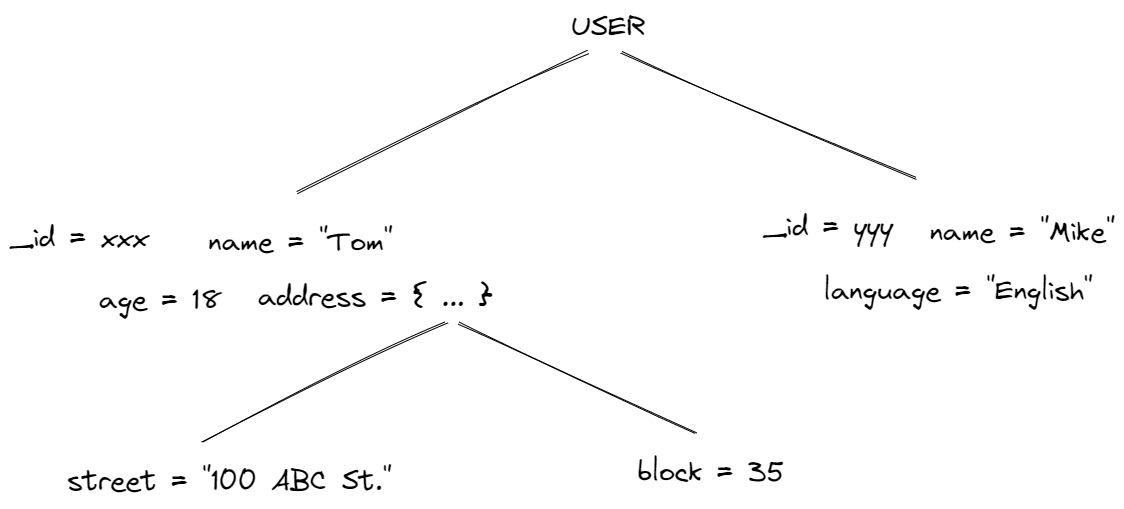
\includegraphics[width=250pt]{chapters/part-3/figures/mongodb_tree.png}
	\caption{A demonstrative example of how MongoDB stores data as (nested) object.} \label{ch:database:mongotree}
\end{figure}

In Fig. \ref{ch:database:mongotree}, a collection ``USER'' is defined. The collection contains two documents. Each document has a few properties. Different document may share common properties such as ``name'' in this example. Each of them can also have unique properties of its own such as ``age'', ``address'' and ``language''. Different properties may have different data types. For example, a property can be string, numeric, or a nested object, or an array of the above. When querying MongoDB, the DBMS is able to return selected properties of documents that meet specific criteria, and sort them in the required order.

\subsection{Data Model}

MongoDB is a document-oriented database program. The data is stored in the format of ``binary JSON'' known as BSON. BSON is an extension of JSON that supports more data types.

\begin{shortbox}
	\Boxhead{JSON VS BSON}
	
	JSON supports the following 6 data types: number, string, boolean, object, array, and null. JSON is text-based, which means that it is essentially a string. It is only a notation of data and does not concern itself with how the data is interpreted in the program that processes the JSON file. For example, ``0'' as a number in a JSON file does not imply whether it is an integer, a 32-bit float, or a 64-bit float.
	
	BSON, on the other hand, is binary-based and hence contains more information. In BSON, more data types are supported, such as different floats, date, timestamp, binary string, regular expression, code, etc. For the same example, ``0'', in BSON different number types are compiled and stored differently. This makes BSON more powerful and efficient (but less intuitive) than JSON.
	
\end{shortbox}

MongoDB uses BSON to store and process data due to its enhanced capability, and uses JSON to display the data.

It is strongly recommended to make the data (document and collection) self-contained. The design of MongoDB architecture should follow depend on how the data would be queried. Data that is accessed together should reside together. This is known as embedding, which adds redundancy to the data storage and make documents bigger, but will make query simpler. Notice that when using embedding, make sure the size of the document is bounded and would not go towards infinity. MongoDB has a maximum $16$MB size limitation for each document.

MongoDB database, unlike relational DB, is by nature not designed for joining. However, MongoDB does support referencing documents and even performing joins (to some extent) through different mechanisms, such as \verb|$lookup| stage in the aggregation pipe.

\section{Installation}

MongoDB, like many other DBMS, has both community and enterprise versions. MongoDB community server can be installed following the instructions in the official website
\begin{lstlisting}
https://www.mongodb.com/try/download/community
\end{lstlisting}
A MongoDB server can host a MongoDB cluster, inside which are many MongoDB databases. Each database can have its own access policy, etc.

To interact with MongoDB DBMS, the quickest way is to use MongoDB shell (also known as ``mongosh''). A description of the shell can be found at
\begin{lstlisting}
https://www.mongodb.com/try/download/shell
\end{lstlisting}
Notice that when installing MongoDB server, it is possible that the server comes with MongoDB Compass, the GUI for MongoDB DBMS. The GUI can also be used to interact with the databases.

Different versions of MongoDB are available. Choose the correct MongoDB version depending on the CPU and the OS of the machine. MongoDB community server installation size is about 500MB.

MongoDB provides enterprise service, MongoDB Atlas, as part of its cloud solution where user can deploy clusters to host databases. With proper gateway setup, the user can connect to MongoDB Atlas clusters from his local server to retrieve data or to manipulate the databases. MongoDB Atlas is briefly introduced in a later section.

\section{MongoDB Shell}

After installing both MongoDB server and MonghDB shell, use
\begin{lstlisting}
$ mongosh
\end{lstlisting}
in the command line to login to the DBMS. JavaScript-like commands are used to manipulate the database, such as creating databases and inserting data.

\subsection{Basic Operation}

The object \verb|db| contains many methods using which the user can access and modify the basic configurations of the database. For example,
\begin{lstlisting}
> db.version()
\end{lstlisting}
gives the version of the database server. More commands can be found using \verb|db.help()|. Some commonly used commands are listed in Table \ref{ch:db:tab:mongodbbasics}.
\begin{table}
	\centering \caption{MongoDB basic commands.}\label{ch:db:tab:mongodbbasics}
	\begin{tabularx}{\textwidth}{lX}
		\hline
		Command & Description \\ \hline
        \verb|db.help()| & Show a list of methods of \verb|db| object. \\ 
		\verb|db.version()| & Show database server version. \\ 
        \verb|db.getUsers()| & Show users. \\ 
        \verb|db.createUser(<content>)| & Create a user. The username, password, roles, etc., needs to be included in the \verb|<content>| area. \\ 
        \verb|db.dropUser(<username>)| & Drop a user. \\ 
        \verb|db.dropDatabase()| & Drop current database. \\ 
		\verb|db.status()| & Show the basic status of the currently selected database, such as its name, number of collections, storage size, etc.  \\
		 \hline
	\end{tabularx}
\end{table}

To display the existing databases, use
\begin{lstlisting}
> show dbs
\end{lstlisting}
On a clean installation, the above should return the 3 default databases, \verb|admin|, \verb|config| and \verb|local|. To switch to a particular database, use
\begin{lstlisting}
> use <database_name>
\end{lstlisting}
Notice that there is no ``create database'' command in MongoDB. To create a database, switch to that database using the above command (even though it does not exist yet), and add some data. The database will be automatically created. This is again a feature closely related to JavaScript.

\subsection{Create Collection and Document}

A MongoDB database contains multiple collections. A collection is similar to a table in an RDB in the sense that it is the collection of data on the same / similar topic. However, unlike tables where schematics such as column names and datatypes are enforced upon creation of the table, a collection does not enforce fields and their data types. The syntax is given below.
\begin{lstlisting}
db.createCollection(<name>, <options>)
\end{lstlisting}

The \verb|<options>| field is optional and allows creating different types of collections, such as time-series collection which is optimized to store time-series sensor data. Probable \verb|<options>| configuration are summarized below.
\begin{lstlisting}
db.createCollection( <name>,
{
	capped: <boolean>,
	timeseries: {                  // Added in MongoDB 5.0
		timeField: <string>,
		metaField: <string>,
		granularity: <string>,
		bucketMaxSpanSeconds: <number>,  // Added in MongoDB 6.3
		bucketRoundingSeconds: <number>  // Added in MongoDB 6.3
	},
	expireAfterSeconds: <number>,
	clusteredIndex: <document>,  // Added in MongoDB 5.3
	changeStreamPreAndPostImages: <document>,  // Added in MongoDB 6.0
	size: <number>,
	max: <number>,
	storageEngine: <document>,
	validator: <document>,
	validationLevel: <string>,
	validationAction: <string>,
	indexOptionDefaults: <document>,
	viewOn: <string>,
	pipeline: <pipeline>,
	collation: <document>,
	writeConcern: <document>
})
\end{lstlisting}
If left empty, a normal collection will be created.

An example of creating a collection inside a database is given below.
\begin{lstlisting}
> use testdb;
> db.createCollection("users");
\end{lstlisting}
Use \verb|show collections| to show the collections in the current database.

\begin{shortbox}
\Boxhead{Should I use semicolon in the end of each MongoDB command?}

If you are using MongoDB shell, then technically speaking, you don't have to. It works both ways. However, if you are using JavaScript environment such as \textit{Node.js} and integrating MongoDB commands as part of the program, you should use semicolon.

For example, to select a database, in MongoDB shell
\begin{lstlisting}
> use myNewDatabase
\end{lstlisting}
or
\begin{lstlisting}
> use myNewDatabase;
\end{lstlisting}
would both work just fine. However, in \textit{Node.js},
\begin{lstlisting}
const newDb = client.db("myNewDatabase");
\end{lstlisting}
the semicolon is highly recommended by JavaScript.

As a conclusion, semicolon is recommended mostly, just to follow the general JavaScript good practice. Although in JavaScript semicolon is also optional due to Automatic Semicolon Insertion (ASI), it is still widely recommended to use semicolon anyway.
\end{shortbox}

Data can be inserted into a collection in the form of documents. It is possible to insert one or multiple documents at a time. To insert documents, first prepare the document in JSON-like format. For example, consider the following documents.
\begin{lstlisting}
{
  name: "Alice",
  age: 20,
  address: "123 Center Park",
  hobbies: ["football", "reading"],
  parents: {
    father: "Chris",
    mother: "Kite"
  }
}

{
  name: "Bob",
  age: Long.fromNumber(25),
  address: "135 Center Park",
  hobbies: BSON.Array(["basketball", "jogging"])
}
\end{lstlisting}
Notice that user ``Alice'' and ``Bob'' in the above example are represented by JSON and BSON respectively. MongoDB uses BSON internally, but it can also take JSON as input, in which case MongoDB driver converts JSON to BSON.

Then use the following syntax to insert the document into the collection.
\begin{lstlisting}
db.<collection_name>.insertOne({...});
db.<collection_name>.insertMany([{...}, {...}, {...}]);
\end{lstlisting}
where \verb|{...}| is the document in JSON or BSON format as shown earlier. To make it more readable, consider do the following instead.
\begin{lstlisting}
const doc = {...};
db.<collection_name>.insertOne(doc);
\end{lstlisting}
which first store the document in \verb|doc|, then pass it to \verb|insertOne()| method. Upon successful insertion, an object id ``\verb|_id|'' will be created automatically and added to the document as another field. The user can also specify \verb|_id| manually. Notice that \verb|_id| serves as the ``primary key'': it must exist and be unique for each document under the same collection.

The above inserting document method creates a collection, if the collection has not been created.

\subsection{Query}

MongoDB uses \verb|find()|, \verb|findOne()| to find documents, where the input is a filter document in the form of a JSON-like string. Details are given below.

To obtain all the document under a collection, use
\begin{lstlisting}
db.getCollection('<collection_name>').find({});
\end{lstlisting}
where an empty query simply matches all documents in the collection. Of course, when \verb|findOne()| is used, it will return only one document.

\begin{shortbox}
\Boxhead{Two Ways to Refer to a Collection}
Notice that
\begin{lstlisting}
db.<collection_name>.<function>()
\end{lstlisting}
is equivalent with
\begin{lstlisting}
db.getCollection('<collection_name>').<function>();
\end{lstlisting}
The first implementation is more convenient while the second more flexible as it supports dynamic naming.
\end{shortbox}

More examples are given below. Assume that there is a collection \verb|posts|, inside which are documents recording the posts by a blogger. Each post may have some comments. The number of comments are recorded in the field \verb|comments| of the documents. To find documents that has a certain field with certain values, use the following
\begin{lstlisting}
db.getCollection('posts').find({comments: 1})
\end{lstlisting}
The above query search documents with field \verb|comments| whose value is $1$ (or whose value is an array that contains $1$ as its element). under collection \verb|posts|. To get those posts with at least $1$ comment, use the following
\begin{lstlisting}
db.getCollection('posts').find({comments: {$gt: 0}})
\end{lstlisting}
where \verb|{$gt: 0}| stands for any value greater than $0$. Commonly seen query operators are given in Table \ref{ch:db:tab:mongodbqueryoperator}, each with an example.

\begin{table}
	\centering \caption{MongoDB basic query operators.} \label{ch:db:tab:mongodbqueryoperator}
	\begin{tabularx}{\textwidth}{llX}
		\hline
		Operator & Description & Example \\ \hline
		\verb|$eq| & Equal & \verb|{age: {$eq: 18}}| \\ 
		\verb|$gt| & Greater than & \verb|{age: {$gt: 18}}| \\ 
		\verb|$gte| & Greater or equal & \verb|{age: {$gte: 18}}| \\ 
		\verb|$lt| & Less than & \verb|{age: {$lt: 18}}| \\ 
		\verb|$lte| & Less or equal & \verb|{age: {$lte: 18}}| \\ 
		\verb|$and| & And & \verb|{$and: [{age: {$gt: 18}}, {sex: 'M'}]}| \\ 
		\verb|$or| & Or &  \verb|{$or: [{age: 18}, {age: 21}]}| \\ 
		\verb|$in| & In & \verb|{name: {$in: ['Alice', 'Bob']}}| \\ 
		\verb|$nin| & Not in & \verb|{name: {$nin: ['Alice', 'Bob']}}| \\
		\hline
	\end{tabularx}
\end{table}

To specifically query for elements in an array, use \verb|$elemMatch| as follows.
\begin{lstlisting}
{ <field>: { $elemMatch: { <query1>, <query2>, ... } } }
\end{lstlisting}
For example,
\begin{lstlisting}
db.scores.find(
	{ results: { $elemMatch: { $gte: 80, $lt: 85 } } }
)
\end{lstlisting}
which returns a document only if: it has a field \verb|results|, and the field \verb|results| is an array, and the array contains at least one such element that is greater or equal than $80$ and less than $85$.

\subsection{Update Document}

Function \verb|updateOne()| is provided to update documents, where the input argument is a tuple containing filtering condition, update and options, following the syntax below.
\begin{lstlisting}
db.<collection_name>.updateOne(filter, update, options)
\end{lstlisting}
Details are given below via an example.
\begin{lstlisting}
db.getCollection('users').updateOne(
	{userId: '0015'},
	{$set: {age: 25}}
);
\end{lstlisting}
The above code query \verb|users| collection, find the document with \verb|userId| being \verb|'0015'|, and change its \verb|age| field to $25$. From this example, it can be seen that the document updating function contains a query and a set of updating operators. Commonly seen updating operators are given in Table \ref{ch:db:tab:mongodbupdateoperator}.

\begin{table}
	\centering \caption{MongoDB basic update operators..}\label{ch:db:tab:mongodbupdateoperator}
	\begin{tabularx}{\textwidth}{llX}
		\hline
		Operator & Description & Example \\ \hline
		\verb|$set| & Add/update field & \verb|{$set: {age: 30 } }| \\ 
		\verb|$unset| & Remove field & \verb|{$unset: {age: ""} }| \\ 
		\verb|$push| & Append to array & \verb|{$push: {age: 25}}| \\ 
		\verb|$inc| & Increase a field & \verb|{$inc: {age: 1} }| \\ 
		\verb|$rename| & Rename field &  \verb|{$rename: {"age": "yearsOld"}}| \\ 
		\verb|$addToSet| & Append to array & \verb|{$addToSet: {hobbies: "reading"}}| \\
		\hline
	\end{tabularx}
	\begin{flushleft}
		\footnotesize
		Notice that \verb|$addToSet| would not append the element if it is already in the array to avoid duplication, while \verb|$push| will append regardless of whether it exists or not.  
	\end{flushleft}
\end{table}

Notice that there is another function, \verb|replaceOne()|, that functions similarly with \verb|updateOne()|. The difference is that \verb|replaceOne()| will replace the entire document, removing all the fields (except \verb|_id|) not mentioned in the update, while \verb|updateOne()| allows editing the mentioned update while leaving unmentioned fields untouched.

It is possible to add \verb|{upsert:true}| as the option to \verb|replaceOne()| function, in which case if no document meets the criteria of the filter, it will create an empty document and implement the updates.

To update documents that meet certain criteria all at once, use \verb|updateMany()| instead. Do note that \verb|updateMany()| is not an atomic operation. It is possible that, for unpredictable reasons, only some of the documents are updated and they will not be rolled back. Use it with caution!

\subsection{Remove Document}

Use either \verb|deleteOne()| or \verb|deleteMany()| to remove documents, with the input the filter document.

\section{MongoDB Compass}

MongoDB Compass is the desktop GUI developed by MongoDB. As a MongoDB client, it can connect to a MongoDB server, either local, remote or MongoDB Atlas, using the connection string. It provides an intuitive user interface that can be used to view and edit the data in the server. 

MongoDB Compass comes with analytical tools and data visualization tools that help the user understand the insight of the data as well as the database structure. It allows the user to define and compose aggregation pipelines that automatically abstract useful aggregated information from the data.

\section{Advanced Query}

It been introduced in the earlier section how \verb|find()| \verb|findOne()| can be used to retrieve documents. The input argument to the above functions is the filter document in JSON-like format, and the documents in the collection that match with the filter document will be returned.

More about query is introduced in this section, such as sorting and limiting the results, returning only selected fields, returning aggregated information, etc.

\subsection{More about \texttt{find()}}

It is worth mentioning that \verb|find()| returns a cursor, but not the documents themselves. One can iterate through the cursor to get all the documents matching the query. This is different from \verb|findOne()| which directly returns a document.

When viewing the data in MongoDB Compass or Atlas, this does not pose an issue. One can simply take \verb|find()| as a function that returns multiple documents. However, in the programming interface, it is important to note the differences between a cursor and a document.

The below are two demonstrative examples how a Python program should treat the returns from \verb|find()| and \verb|findOne()| differently. The same idea applies to other programming languages as well.

\begin{lstlisting}
from pymongo import MongoClient

def find_users():
	client = MongoClient('mongodb://localhost:27017/')
	db = client.mydatabase
	collection = db.users

	cursor = collection.find({ 'age': { '$gte': 18 } })

	# Iterate over the cursor
	for doc in cursor:
		print(doc)
	
	# Alternatively, convert to a list
	results = list(cursor)
	print(results)

	client.close()
\end{lstlisting}

\begin{lstlisting}
from pymongo import MongoClient

def find_one_user():
	client = MongoClient('mongodb://localhost:27017/')
	db = client.mydatabase
	collection = db.users

	# Find one document
	user = collection.find_one({ 'name': "John Doe" })
	print(user)

	client.close()
\end{lstlisting}

Since a cursor, instead of the documents themselves, is returned, we can perform further actions on the return such as sorting the result, etc.

\subsection{Sorting}

Use the following syntax to retrieve and sort the return.
\begin{lstlisting}
cursor.sort({<field>:<value>})
\end{lstlisting}
which sorts the result according to \verb|<field>|. The value ``$1$'' or ``$-1$'' represents the sorting order, either ascending or descending, respectively.

\subsection{Limiting the Number of Returns}

When it is unnecessary to return all the details of all the documents fulfilling the query criteria, it is possible to limit the field number of returned documents which is often helpful with improving the data processing efficiency.

It is possible to limit the number of documents in the returns to improve the query efficiency. This is often used with the \verb|sort()| method. The syntax is as follows.
\begin{lstlisting}
cursor.sort({<field>:<value>}).limit(<number>)
\end{lstlisting}
where \verb|<number>| specifies the number of returns.

\subsection{Limiting the Fields of Returns}

Notice that the full syntax of \verb|find| is
\begin{lstlisting}
db.collection.find( <query>, <projection>, <options> )
\end{lstlisting}
The second argument, \verb|<projection>|, is used to indicate which fields of the documents should be returned. If left blank as by the default, all the fields of the documents will be returned. Notice that the same applies to \verb|findOne()| method.

For example,
\begin{lstlisting}
cursor = collection.find({'age': {'$gte': 18}}, {name:1, age: 1})
\end{lstlisting}
will return the names and ages of all the users whose age is greater than or equal to $18$. By using
\begin{lstlisting}
{ <field1>: <value>, <field2>: <value> ... }
\end{lstlisting}
with \verb|<value>| be either $1$ or $0$, one can control which fields to be included or excluded respectively. The value $0$ is often used with the \verb|_id| field which is always returned unless specifically required not to. Notice that the \verb|<field>| in the syntax can also contain sub fields, in which case quotation marks \verb|"<field>.<subfield>"| must be used.

With some more advanced setups, \verb|<projection>| can also be used to specify what elements in an array to return, and more. For details, check the user manual of \verb|db.collection.find()| function.

\subsection{Counting the Number of Returns}

Consider counting the number of documents fulfilling a particular filter document. Use
\begin{lstlisting}
db.<collection>.countDocuments( <query>, <options> )
\end{lstlisting}

\section{Sharding and Indexing}

Given that MongoDB is often used with big data such as web data or IoT data, efficient query from massive data pool becomes critical. MongoDB implements a few technologies to speed up the query such as sharding and indexing.

\subsection{Sharding}

Sharding is a method of distributing data across multiple servers or instances. In MongoDB, a shard consists of a subset of the total dataset, and each shard is responsible for managing a portion of the data. This distribution allows MongoDB to scale horizontally by adding more servers, thereby spreading the load and the data volume across a cluster. When a query is executed, it only needs to be processed by the shards that contain relevant data, rather than the entire dataset. This can significantly reduce query times in a large, distributed system. Sharding is particularly useful for very large datasets and high throughput operations, where a single server would not be sufficient to store the data or provide acceptable performance.

\subsection{Indexing}

Indexing is a technique used to speed up the retrieval of documents within a database. MongoDB uses indexes to quickly locate a document without having to scan every document in a collection. Indexes are a critical component of database optimization, as they can drastically reduce the amount of data MongoDB needs to retrieve documents for a query. 

When a filter such as \verb|find()|, \verb|findOne()|, or in an aggregation pipeline, \verb|$match| are used, MongoDB automatically utilizes the available indexes to speed up the query, making it more efficient.

When projection is used to limit the fields to be returned, and if it happens that all the returned fields are part of the index, MongoDB would not need to look back into the documents. In this case, the query speed can be significantly faster.

\begin{shortbox}
\Boxhead{MongoDB's B-Tree}

MongoDB primarily uses B-Tree data structures for its indexes. A B-Tree is a self-balancing tree data structure that maintains sorted data in a way that allows searches, sequential access, insertions, and deletions in logarithmic time. The ``B'' in B-Tree stands for ``balanced'' and indicates that the tree is designed to keep the data balanced, ensuring that operations are efficient as the dataset grows. The B-Tree structure allows MongoDB to perform efficient query. Instead of scanning every document in a collection, MongoDB can use the B-Tree index to quickly navigate through a small subset of the data to find the documents that match the query criteria.
\end{shortbox}

However, index by itself is also an argument data structure and it consumes disk and memory space. Each time there is a write operation, the index needs to be updated. Therefore, a very complicated index schema slows down data insertion. It is critical to design appropriate index to optimize the overall performance of the database.

The default index for a collection is ``\verb|_id|'', a compulsory and unique field required by MongoDB. The user can also define index of different types. User-defined index can be unique or non-unique. The index of a collection can be created when the collection is empty, or when there are already some documents.

A MongoDB collection can have multiple indexes, and when you perform a query, MongoDB will choose the most suitable index to use based on the query's criteria.

\subsection{Simple and Compound Index}

There are many options when creating the user-defined index. The following function 
\begin{lstlisting}
db.collection.createIndex(<keys>, <options>, <commitQuorum>)
\end{lstlisting}
creates a user-defined index. A single or a compound of multiple fields in a collection can be used as the index using
\begin{lstlisting}
db.collection.createIndex(
	{
		<field1>: 1,
		<field2>: -1,
		...
	}
)
\end{lstlisting}
Those fields assigned with ``$1$'' or ``$-1$'' is listed as the ascending and descending index. The choice of order determines how the index sorts the indexed field's values, which can affect the performance of certain queries.

The data types of the selected field(s) can be scalar, string, or even a nested object. MongoDB has an internal mechanism that can convert different data types into a format that can be indexed and sorted efficiently.

The order of fields in a compound index can significantly impact query performance in MongoDB. Following the principle of ``equality, sort, range'' when defining compound indexes is a good practice to optimize queries.

\begin{itemize}
	\item Equality. Fields that are used in equality conditions (\verb|=|) should come first in the index. These fields are used to narrow down the search space quickly.
	\item Sort. Fields that are used for sorting the results should come next. Sorting fields in the index help MongoDB to efficiently retrieve documents in the desired order without additional sorting.
	\item Range. Fields that are used in range queries (\verb|<|, \verb|<=|, \verb|>|, \verb|>=|, \verb|$in|, etc.) should be placed last. Range queries can benefit from being at the end of the index because they can take advantage of the already reduced search space provided by the equality and sort fields.
\end{itemize}

It is possible to use the \verb|<options>| argument to set additional constraints to the index, for example, to enforce its value to be unique.

\subsection{Multi-key Index}

When defining index on an array field, the index is known as multi-key index. Like the scalar fields, multi-key index can also be both single or compound. It is also possible to mix scalar keys with array keys.

Syntax wise, defining a multi-key index looks similar with defining a regular single or compound index as follows.
\begin{lstlisting}
db.collection.createIndex(
	{
		<scalar field1>: 1,
		<scalar field2>: 1,
		<array field>: 1
	}
)
\end{lstlisting}
The only limitation is that there can be only one array key per index.

Behind the screen, MongoDB treats each element in the array key as a separate index value. Likewise, each element in the array of the index can be scalar, string, or nested object.

\subsection{Hide and Remove Index}

It is not recommended to modify the index of a collection frequently, as deleting and recreating index take time and resources. Sometimes we do need to remove a redundant index if it is adding too much writing cost.

It is possible to test the query performance if an index were to be removed before actually removing it. This can be done by temporarily hide the index. MongoDB would not use hidden index in the query, though it will still update the index when new data is written in.

To hide an index, use
\begin{lstlisting}
db.<collection>.hideIndex(<index>)
\end{lstlisting}
where \verb|<index>| can be either a string or a document that indicates the status of the index. An example is given below.

Consider a restaurant collection, with the following user-defined index:
\begin{lstlisting}
db.restaurants.createIndex( { borough: 1, ratings: 1 } );
\end{lstlisting}
Now the collection should have 2 indexes, the first the default index with \verb|_id| field, the second the compound index composed of \verb|borough| and \verb|ratings| fields.

The user-defined compound index can be hidden by one of the two syntax below.
\begin{lstlisting}
db.restaurants.hideIndex( "borough_1_ratings_1" ); // option 1
db.restaurants.hideIndex( { borough: 1, ratings: 1 } ); // option 2
\end{lstlisting}

After hiding the user-defined index, the index status becomes
\begin{lstlisting}
[
	{
		"v" : 2,
		"key" : {
			"_id" : 1
		},
		"name" : "_id_"
	},
	{
		"v" : 2,
		"key" : {
			"borough" : 1,
			"ratings" : 1
		},
		"name" : "borough_1_ratings_1",
		"hidden" : true
	}
]
\end{lstlisting}

To remove an index instead of hiding it, use \verb|dropIndex()| instead of \verb|hideIndex()|. A similar-looking command \verb|dropIndexes()| allows removing multiple indexes at the same time.

\subsection{Performance Evaluation with Index}

To check the indexes of a system, use
\begin{lstlisting}
db.collection_name.getIndexes()
\end{lstlisting}
The index can also be viewed from the graphical UI.

Consider using \verb|explain()| function as follows when carrying out a find operation.
\begin{lstlisting}
db.<collection>.explain().find()
\end{lstlisting}
which will list down the down-to-the-ground stages to carry out the query. Apply the same query to two identical collections, one with index and the other without on different scenarios where:
\begin{enumerate}
	\item The filter document and the projection only contains indexed fields.
	\item The filter document contains indexed fields, but the returns require more fields.
	\item The filter document does not contain indexed fields.
\end{enumerate}
and compare the differences.

\section{Third-Party Connection}

Both MongoDB shell CLI and MongoDB Compass GUI can connect to MongoDB as introduced in earlier sections. Third-party applications can also connect to MongoDB. As of this writing, MongoDB supports libraries for the following developing languages:
\begin{multicols}{4}
\begin{itemize}
	\item \verb|C/C++|
	\item \verb|C#|
	\item \verb|Go|
	\item \verb|Java|
	\item \verb|Kotlin|
	\item \verb|Node.js|
	\item \verb|PHP|
	\item \verb|Python|
	\item \verb|Ruby|
	\item \verb|Rust|
	\item \verb|Scala|
	\item \verb|Swift|
	\item \verb|TypeScript|
\end{itemize}
\end{multicols}
A full list can be found at
\begin{lstlisting}
https://www.mongodb.com/docs/drivers/
\end{lstlisting}

Here is a quick example to connect to MongoDB using Python library \verb|PyMongo|. The installation of the library is not given.
\begin{lstlisting}
import pymongo
from pymongo import MongoClient

def initialize_mongodb_collection(connection_string, database_name, collection_name, index_field):
	client = MongoClient(connection_string)
	db = client[database_name]
	collection = db[collection_name]
	collection.create_index(index_field)

def push_to_mongodb(connection_string, database_name, collection_name, data):
	client = MongoClient(connection_string)
	try:
		db = client[database_name]
		collection = db[collection_name]
		if isinstance(data, dict):
			result = collection.insert_one(data)
			print(result.acknowledged)
			elif isinstance(data, list):
			result = collection.insert_many(data)
			print(result.acknowledged)
		else:
			raise Exception("Data should be a dictionary or a list of dictionaries")
		client.close()
	except Exception as e:
		raise Exception("Unable to insert the document: ", e)

def pull_from_mongodb(connection_string, database_name, collection_name, query_dict):
	results = None
	client = MongoClient(connection_string)
	try:
		db = client[database_name]
		collection = db[collection_name]
		results = collection.find(query_dict) # return iterative object
		client.close()
	except Exception as e:
		raise Exception("Unable to insert the document: ", e)
	return results

\end{lstlisting}
A full instruction to execute the above example can be found at
\begin{lstlisting}
https://www.mongodb.com/docs/languages/python/pymongo-driver/current/get-started/
\end{lstlisting}

\section{Aggregation Framework}

Aggregation is the analysis and summary of data. MongoDB, like many other databases, provides powerful tools to perform aggregation functions such as counting the number of documents, calculating the sum / average of a particular field of filtered documents, etc. Beyond that, MongoDB allows the user to define a pipeline composed of a sequence of data processing procedures for aggregation. This enables autonomous data processing and analysis, and it is useful especially for big data applications. This feature, known as the data aggregation framework or data aggregation pipeline, is one of the most powerful and useful features that MongoDB offers.

Aggregation pipeline is supported in all MongoDB tiers, including MongoDB Community, Enterprise and Atlas.

\subsection{Aggregation Pipeline Syntax}

To apply different aggregation functions, use \verb|aggregate()| as follows.
\begin{lstlisting}
db.<collection>.aggregate( <pipeline>, <options> )
\end{lstlisting}
where \verb|<pipeline>| is usually an array that contains a sequence of aggregation operations including filter, sorting, grouping and transforming, which may look like the following
\begin{lstlisting}
db.<collection>.aggregate([
	{
		$<stage>: {<expression>}
	},
	{
		$<stage>: {<expression>}
	},
	{
		$<stage>: {<expression>}
	}
])
\end{lstlisting}

An example is given blow.
\begin{lstlisting}
db.orders.insertMany( [
	{ _id: 0, name: "Pepperoni", size: "small", price: 19,
		quantity: 10, date: ISODate( "2021-03-13T08:14:30Z" ) },
	{ _id: 1, name: "Pepperoni", size: "medium", price: 20,
		quantity: 20, date : ISODate( "2021-03-13T09:13:24Z" ) },
	{ _id: 2, name: "Pepperoni", size: "large", price: 21,
		quantity: 30, date : ISODate( "2021-03-17T09:22:12Z" ) },
	{ _id: 3, name: "Cheese", size: "small", price: 12,
		quantity: 15, date : ISODate( "2021-03-13T11:21:39.736Z" ) },
	{ _id: 4, name: "Cheese", size: "medium", price: 13,
		quantity:50, date : ISODate( "2022-01-12T21:23:13.331Z" ) },
	{ _id: 5, name: "Cheese", size: "large", price: 14,
		quantity: 10, date : ISODate( "2022-01-12T05:08:13Z" ) },
	{ _id: 6, name: "Vegan", size: "small", price: 17,
		quantity: 10, date : ISODate( "2021-01-13T05:08:13Z" ) },
	{ _id: 7, name: "Vegan", size: "medium", price: 18,
		quantity: 10, date : ISODate( "2021-01-13T05:10:13Z" ) }
] )
	
db.orders.aggregate( [
	// Stage 1: Filter pizza order documents by pizza size
	{
		$match: { size: "medium" }
	},
	// Stage 2: Group remaining documents by pizza name and calculate total quantity
	{
		$group: { _id: "$name", totalQuantity: { $sum: "$quantity" } }
	}
] )
\end{lstlisting}
where both \verb|$match| and \verb|$group| are commonly used stages.

And the return is a cursor pointing to the following array of documents
\begin{lstlisting}
[
	{ _id: 'Cheese', totalQuantity: 50 },
	{ _id: 'Vegan', totalQuantity: 10 },
	{ _id: 'Pepperoni', totalQuantity: 20 }
]
\end{lstlisting}
The return of an aggregation pipeline can be returned to the program for further data mining. It can also create new documents or modify existing documents.

Notice that the design of pipeline affects the performance of the query. There are many supported stages, each with a different list of input arguments. A full list of supported stages can be found from MongoDB's user manual at \cite{mongodb2024aggregation}
under ``Aggregation Stages''. Calculations can be performed along with the aggregation pipeline. The calculations are triggered by aggregation operators. A full list of supported aggregation operators can be found from MongoDB's user manual at \cite{mongodb2024aggregationoperators} under ``Aggregation Operators''.

It is highly recommended that one should read through MongoDB's user manual to learn the aggregation framework. For the convenience of the reader, commonly used stages are introduced as follows.

\subsection{Stage: \texttt{\$match}}

The \verb|$match| stage filters the documents to pass only the documents that match the specified conditions to the next pipeline stage. A general syntax is given below.
\begin{lstlisting}
	{$match: <filter>}
\end{lstlisting}

The \verb|$match| stage should be used in early steps to make the pipeline more efficient.

\subsection{Stage: \texttt{\$group}}

The \verb|$group| stage separates documents into groups according to a ``group key''. The output is one document for each unique group key. Use \verb|null| as the group key to group all documents into a single group. Consequent aggregations are then performed per group.

A general syntax is given below.
\begin{lstlisting}
{
	$group:
	{
		_id: <expression>, // Group key
		<field1>: { <accumulator1> : <expression1> },
		...
	}
}
\end{lstlisting}
where \verb|<accumulator>| indicates what to calculate on the grouped information to put into the \verb|field|. For example, the accumulator can be \verb|$count|.

The following is an example. Let there be a collection ``commodity'', inside which each document represents a product, and has the following 3 fields: ``item'' (item name), ``price'' (unit price) and ``quantity'' (the sold number). The target is to calculate the sold total price for each product.
\begin{lstlisting}
{
	$group :
	{
		_id : "$item",
		totalSaleAmount: { $sum: { $multiply: [ "$price", "$quantity" ] } }
	}
}
\end{lstlisting}
Do notice that to refer to the field name in the documents, use \verb|"$<fieldname>"|.

The return of the above may look like the following
\begin{lstlisting}
[
	{ _id: "apple", totalSaleAmount: 50 },
	{ _id: "banana", totalSaleAmount: 45 }
]

\end{lstlisting}

If \verb|null| were used as the group key, the return would have been
\begin{lstlisting}
[
	{ _id: null, totalSaleAmount: 95 }
]
\end{lstlisting}

To count the number of documents in each group and put it as an additional field, consider using \verb|$sum| as follows.
\begin{lstlisting}
{
	$group: {
		_id: <expression>, // Group key
		count: { $sum: 1 } // Accumulator to count documents
	}
}
\end{lstlisting}

\subsection{Stage: \texttt{\$sort}}

The \verb|$sort| stage sorts the documents in either ascending order or descending order for further processing in the pipeline. The \verb|$sort| stage is sometimes used before \verb|$limit| stage.

A general syntax is given below.
\begin{lstlisting}
{
	$sort:
	{
		<field1>: 1 // or -1
	}
}
\end{lstlisting}
where ``$1$'' and ``$-1$'' indicate the ascending and descending order with respect to the field.

\subsection{Stage: \texttt{\$limit}}

The \verb|$limit| stage selects and filters the first a few items from the pipeline. The input argument is simply a positive integer, as shown in the below example.
\begin{lstlisting}
{
	$limit: 3
}
\end{lstlisting}

\subsection{Stage: \texttt{\$set}}

The \verb|$addFields| or \verb|$set| stage (alias of each other) is used to modify or add fields in the pipeline, using the following syntax.
\begin{lstlisting}
{
	$set:
	{
		<field1>: <new value>,
		<field2>: {<expression>},
		...
	}
}
\end{lstlisting}
The assignment can be either a value or an expression, such as rounding, multiplying by a gain, etc. A list of supported arithmetic aggregation functions is given in Table \ref{tab:mongodb_arithmetic_aggregation}.

\begin{table}
	\centering \caption{MongoDB arithmetic aggregation functions.}\label{tab:mongodb_arithmetic_aggregation}
	\begin{tabularx}{\textwidth}{lX}
		\hline
		Name & Description \\ \hline
		\verb|$abs| &	Returns the absolute value of a number. \\
		\verb|$add| &	Adds numbers to return the sum, or adds numbers and a date to return a new date. If adding numbers and a date, treats the numbers as milliseconds. Accepts any number of argument expressions, but at most, one expression can resolve to a date. \\
		\verb|$ceil| &	Returns the smallest integer greater than or equal to the specified number. \\
		\verb|$divide| &	Returns the result of dividing the first number by the second. Accepts two argument expressions. \\
		\verb|$exp| &	Raises e to the specified exponent. \\
		\verb|$floor| &	Returns the largest integer less than or equal to the specified number. \\
		\verb|$ln| &	Calculates the natural log of a number. \\
		\verb|$log| &	Calculates the log of a number in the specified base. \\
		\verb|$log10| &	Calculates the log base 10 of a number. \\
		\verb|$mod| &	Returns the remainder of the first number divided by the second. Accepts two argument expressions. \\
		\verb|$multiply| &	Multiplies numbers to return the product. Accepts any number of argument expressions. \\
		\verb|$pow| &	Raises a number to the specified exponent. \\
		\verb|$sqrt| &	Calculates the square root. \\
		\verb|$subtract| &	Returns the result of subtracting the second value from the first. If the two values are numbers, return the difference. If the two values are dates, return the difference in milliseconds. If the two values are a date and a number in milliseconds, return the resulting date. Accepts two argument expressions. If the two values are a date and a number, specify the date argument first as it is not meaningful to subtract a date from a number. \\
		\verb|$trunc| &	Truncates a number to its integer. \\
		\hline
	\end{tabularx}
\end{table}

\subsection{Stage: \texttt{\$count}}

The \verb|&count| stage counts the number of the documents passing through the pipeline, and put the number into a field.
\begin{lstlisting}
{
	$count: <field>
}
\end{lstlisting}

An example is given below
\begin{lstlisting}
db.scores.aggregate([
	{
		$match: {
			score: {
				$gt: 80
			}
		}
	},
	{
		$count: "passing_scores"
	}
])
\end{lstlisting}
which count the number of students whose score is greater than $80$. Notice that when using \verb|$group| stage, \verb|count: {$sum: 1}| can be used to count the number of elements in each group. Though both methods counts the number of documents, they are used in different contexts.

\subsection{Stage: \texttt{\$project}}

The \verb|$project| stage changes the shape of the data in the pipeline. It selects which fields to be displayed. In many occasions it is used near the end of the pipeline, right before the data comes out of the pipeline. 

A general syntax looks like the following.
\begin{lstlisting}
{
	$project:
	{
		<field1>: 1,
		<field2>: 0,
		<field3>: <new value>,
		...
	}
}
\end{lstlisting}
where ``$1$'' and ``$-1$'' are used to either include or exclude a field. It can also create new fields or overwrite an existing field, in which case the value of the new fields needs to be specified.

\subsection{Stage: \texttt{\$out}}

The \verb|&out| stage creates a new collection or overwrite an existing collection using the aggregation pipeline result. If \verb|&out| is used, it should be the last stage.
\begin{lstlisting}
{
	$out:
	{
		db: "<database name>",
		coll: "<collection name>"
	}
}
\end{lstlisting}
or
\begin{lstlisting}
{
	$out: "<collection name>"
}
\end{lstlisting}

\section{MongoDB Atlas}

MongoDB Atlas is the MongoDB cloud-based serverless solution. It allows the user to deploy MongoDB on the cloud. The user has the freedom to choose the base cloud service provider including AWS, Azure and Google Cloud. Thanks to Altas, the user has the flexibility to seamlessly change cloud service providers and service tiers without downtime. 

In addition to just a host of the database, Atlas provides varieties of tools that helps the developer to develop applications using the database, such as a centralized cloud-based dashboard, autonomous synchronization with edge devices, etc. Some other examples include Atlas data lake which is optimized for analytical queries. Big data can be stored in Atlas data lake, from where analytical information can be retrieved. Atlas federation allows seamlessly query, transform, and aggregate data from one or more MongoDB Atlas databases and cloud object storage offerings. Atlas chart provides rich tools for MongoDB data visualization. There are many more tools.

As of this writing, Atlas allows the user to choose from 3 different storage tiers:
\begin{itemize}
  \item Shared: the database is stored on shared servers; the user can select the server provider from AWS, Azure and Google Cloud
  \begin{itemize}
    \item M0: free, $512$MB
    \item M2: 2GB, \$$9$ / month
    \item M5: 5GB, \$$25$ / month
  \end{itemize}
  \item Dedicated: the database is stored on dedicated servers with dedicated storage, RAM and multi-core CPUs; $10$GB to $4$TB; \$$0.08$ / hour - \$$33.26$ / hour
  \item Serverless: the database is provided as a microservice, and it automatically scales up and down based on use; up to 1TB; the cost depends on the amount of stored data, the number of read and write operations, the computational cost of backups, etc.
\end{itemize}

\subsection{MongoDB Atlas Dashboard}

To use MongoDB Atlas, register an account with MongoDB Atlas.

Create a database cluster. Select the pricing tier for the database cluster, create a user with admin role and assign him a password, and configure the database cluster access gateway (i.e., a list of IP address that can access the database cluster). Upon creation of the database cluster, the user gains the access to MongoDB Atlas dashboard. The browser-based MongoDB Atlas dashboard can be used to view, add, edit and remove documents, collections and databases.

The newly created database cluster is emply and has no databases, collections or documents. For tutorial purpose, Altas provides a sample database cluster. One can import the data in the sample database cluster into the created empty database cluster. 

MongoDB Atlas dashboard provides data explorer tool that allows the user to view and edit the database directly, without using CLI or code. One can also filter documents from a collection by filtering the fields of the documents. Of course, MongoDB Atlas also provides connection string so that the user can connect to it remotely using CLI, from MongoDB Compass, or from third-party applications.

The following screenshot in Fig. \ref{ch:database:atlasdashboard} gives MongoDB Atlas dashboard. The database cluster, user and gateway can be viewed and configured from the dashboard.

\begin{figure}[htbp]
	\centering
	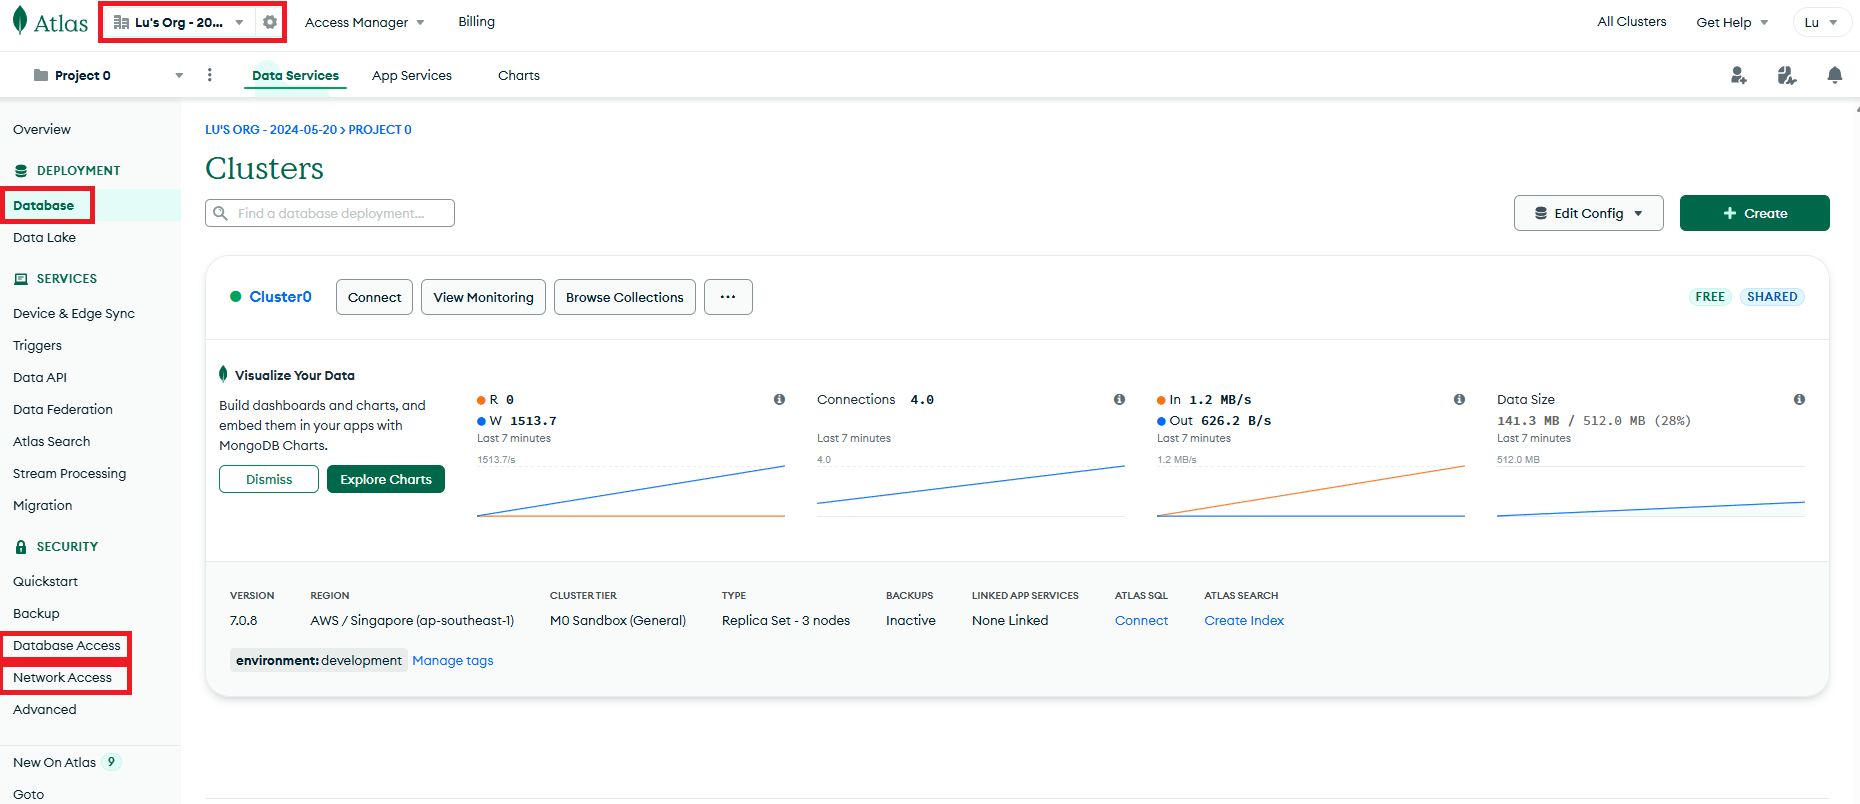
\includegraphics[width=\textwidth]{chapters/part-3/figures/atlas_dashboard.png}
	\caption{A demonstration of MongoDB Atlas dashboard.} \label{ch:database:atlasdashboard}
\end{figure}

To view collections and query for documents, click ``Browse Collections'' in Fig. \ref{ch:database:atlasdashboard} which gives Fig. \ref{ch:database:atlasdashboard2}. This sample database cluster contains multiple databases, each database with several collections, as shown by Fig. \ref{ch:database:atlasdashboard2}.

\begin{figure}[htbp]
	\centering
	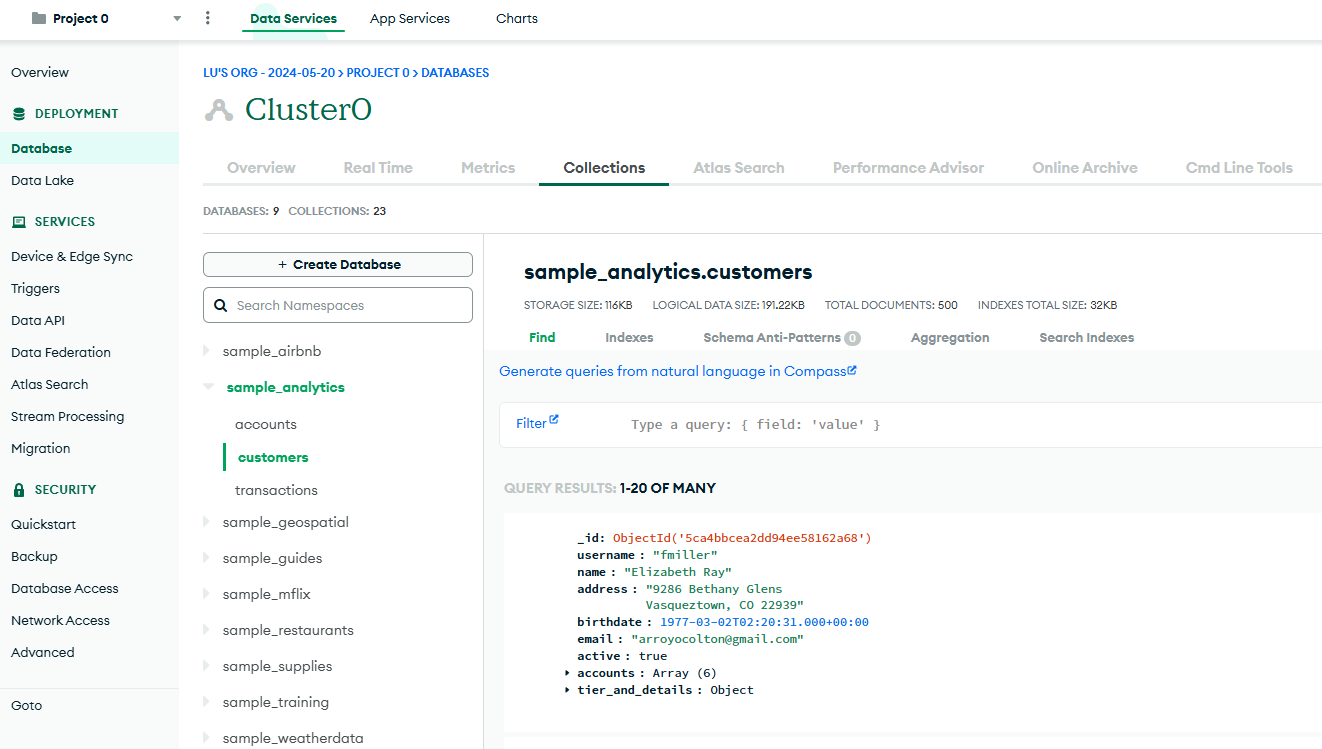
\includegraphics[width=\textwidth]{chapters/part-3/figures/atlas_dashboard_2.png}
	\caption{A demonstration of MongoDB Atlas dashboard where the databases and collections under ``\texttt{Project 0}'', ``\texttt{Cluster0}'' are browsed. Database ``\texttt{sample\_analytics}'', collection ``\texttt{customers}'' is selected. There are $500$ documents under this collection.} \label{ch:database:atlasdashboard2}
\end{figure}

\subsection{Connection String}

Database connection string allows a client to connect to a database server. MongoDB Atlas provides two connection string formats, namely the standard format and the DNS seed list format. The connection string of MongoDB Atlas can be retrieved from the dashboard by clicking ``Connect'' in Fig. \ref{ch:database:atlasdashboard}. It is possible to connect to MongoDB Atlas from:
\begin{itemize}
  \item MongoDB Shell (MongoDB's CLI)
  \item MongoDB Compass (MongoDB's desktop client GUI)
  \item User applications
\end{itemize}
Simply follow the instructions to connect to Atlas from one of the above entries. Notice that as a prerequisite, MongoDB Atlas needs to have the gateway policy to allow such connectivity.

A connection string may look like the following
\begin{lstlisting}
mongodb+srv://<username>:<password>@<server-dns>/?authSource=admin&replicaSet=myRepl
\end{lstlisting}

\subsection{Atlas Search}

Altas search is a powerful full-text search feature provided by Atlas that can access the documents and search for information based on relevance.  It is built on top of Apache Lucene, a high-performance, full-featured text search engine library, and is designed to offer advanced search capabilities beyond the basic query. 

Notice that Atlas search is NOT database query based on \verb|find()|, nor AI-encoder-decoder based semantic search. Unlike traditional MongoDB queries which are based on exact matches or range conditions, Atlas Search provides relevance-based search. This means that search results are ranked by how well they match the search criteria, similar to how web search engines work. From this point of view, Atlas search is more business-user friendly, while MongoDB database search is more for developers and applications.

Atlas search, as well as Apache Lucene, uses search index to collect and parse the data to improve search efficiency. Do NOT confuse the search index with the MongoDB collection index introduced in earlier sections, as they are fundamentally different.

The remaining of this section introduces the use of Atlas search. Notice that Atlas search is power and flexible. Only a scratch is covered here.

\vspace{0.1in}
\noindent \textbf{Create Search Index and Test Atlas Search}
\vspace{0.1in}

Don't confuse Atlas search index or Apache Lucene index with MongoDB collection index. They function fundamentally differently. The purpose of the search index is to provide advanced full-text search capabilities, as so required by Apache Lucene.

MongoDB Atlas dashboard provides a GUI to create and manage search indexes for collections, as shown by the demonstration in Fig. \ref{ch:database:atlassearchdashboard}. All configurations such as index analyzer, search analyzer, etc., are left as default in this example. It will take some time when setting up the search index. 

\begin{figure}[htbp]
	\centering
	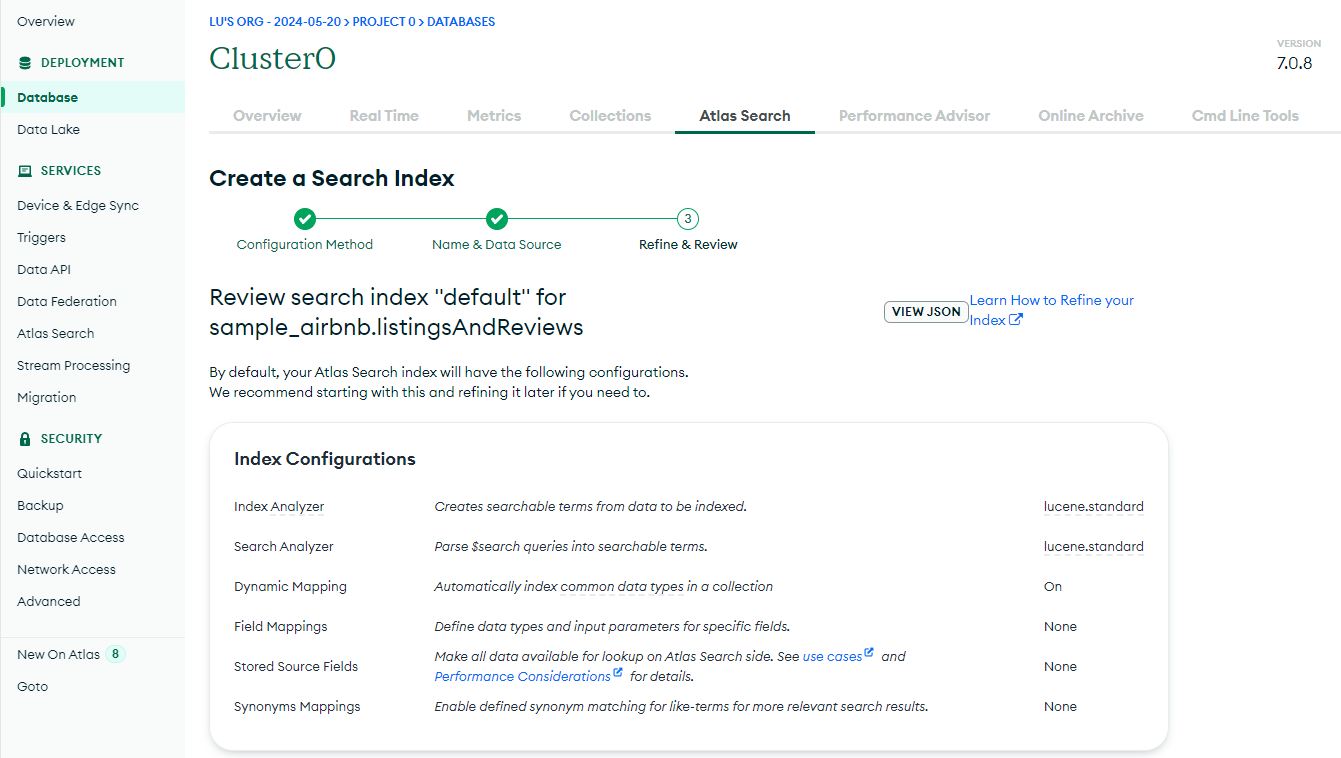
\includegraphics[width=\textwidth]{chapters/part-3/figures/atlas_search_dashboard.png}
	\caption{Atlas search set up search index using the dashboard.} \label{ch:database:atlassearchdashboard}
\end{figure}

With this setup, we can search the documents as if we were using a web searching engine. An example is given in Fig. \ref{ch:database:atlassearchtest}. The most relevant documents with the keyword ``big room'' is returned. Each returned document corresponds with a score.

\begin{figure}[htbp]
	\centering
	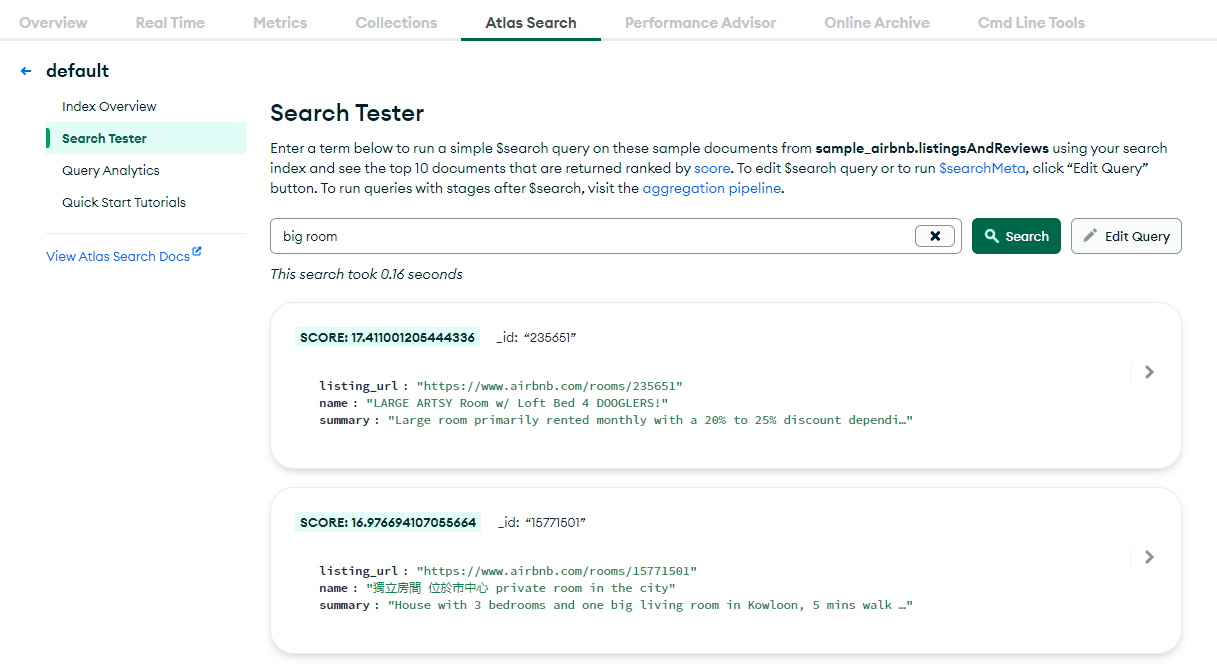
\includegraphics[width=\textwidth]{chapters/part-3/figures/atlas_search_test.png}
	\caption{Atlas search test.} \label{ch:database:atlassearchtest}
\end{figure}

The default search index, as shown by the above example, uses dynamic mapping. It index all the fields in the collection. If we have priori knowledge about which field(s) to query, we can use static mapping which usually returns results faster. 

To use static mapping, click the button ``refine your index'' during the search index creation, disable dynamic mapping, and add fields of interest following the instruction.

\vspace{0.1in}
\noindent \textbf{Use Atlas Search in the Aggregation Pipeline}
\vspace{0.1in}

With Atlas, we can add Atlas search as part in the aggregation pipeline. The associated stage is \verb|$search|. It must be used together with Atlas search. The syntax looks like the following.

\begin{lstlisting}
{
	$search: {
		"index": "<index-name>",
		"<operator-name>"|"<collector-name>": {
			<operator-spec>|<collector-spec>
		},
		"highlight": {
			<highlight-options>
		},
		"concurrent": true | false,
		"count": {
			<count-options>
		},
		"searchAfter"|"searchBefore": "<encoded-token>",
		"scoreDetails": true| false,
		"sort": {
			<fields-to-sort>: 1 | -1
		},
		"returnStoredSource": true | false,
		"tracking": {
			<tracking-option>
		}
	}
}
\end{lstlisting}
which can be defined in the Atlas dashboard under ``Collections'', ``Aggregation''.

\subsection{Schema Pattern}

The schema pattern is the guidance of designing good MongoDB architecture. Schema anti-pattern, on the other hand, refers to the architecture design that causes sub optimal performance.

Commonly seen schema anti-patterns include:
\begin{itemize}
	\item Massive arrays.
	\item Massive number of collections.
	\item Bloated documents.
	\item Unnecessary indexes.
	\item Queries without indexes.
	\item Data that is accessed together but not stored together.
\end{itemize}

Atlas provides tools to help identify these schema anti-patterns. There are different ways to tackle each of these issues.

\chapter{Non-RDB Example: Redis}

Redis, short for \textit{REmote DIctionary Server}, is an open-source in-memory distributed key-value database.

The community version of Redis is free of cost and can be installed on multiple platforms. Redis Cloud, on the other hand, is a paid service with additional features and can be deployed on various cloud platforms such as AWS, Azure, and Google Cloud.

\section{Brief Introduction to Redis}

Redis is an open-source in-memory distributed database. It is a NoSQL database and does not structure and store data in tables. Unlike MongoDB, which stores data using self-contained documents, Redis stores data in key-value pairs. Redis is renowned for its support of in-memory data storage, significantly speeding up data storage, query, and processing. As a result, it is often used as a lightweight data caching tool or a message broker.

The features of Redis are summarized as follows:
\begin{itemize}
	\item In-memory storage: This speeds up reading and writing operations.
	\item Persistence: While primarily an in-memory database, Redis offers various ways to persist data on disk without significantly compromising performance.
	\item Complex data structures and associated atomic operations: Though Redis is a key-value store, it supports more complex data structures than just simple key-value pairs.
	\item High availability via replicas: Redis can create replicas to ensure high availability.
	\item Distributed storage via horizontal partitioning: Redis supports horizontal partitioning for distributed storage.
	\item Lightweight: Redis is designed to be lightweight, making it efficient and easy to use.
\end{itemize}

A potential drawback of Redis is that when it is used in-memory, the data may be lost in the event of a system shutdown. For this reason, a popular way of using Redis is to let it sit between the user and a persistent database running in the backend. In this architecture, Redis serves as a fast-responding replica to enhance the user experience. When the data to retrieve is in Redis, the system does not need to query the backend database and it can return the result in milliseconds, which otherwise would have cost hundreds or thousands of milliseconds.

\section{Installation}

To install Redis on a Linux machine, simply use the package manager of the machine. For example, for RHEL, do the following
\begin{lstlisting}
$ sudo dnf install redis
\end{lstlisting}
to install Redis, and use
\begin{lstlisting}
$ redis-server
\end{lstlisting}
to start the Redis server. Upon starting of Redis, the port number and the process id will pop up. By default, it runs on port $6379$.

To login to Redis on the host machine, simply use
\begin{lstlisting}
$ redis-cli
\end{lstlisting}
to open the CLI to the database. The CLI prompt that looks like
\begin{lstlisting}
127.0.0.1:6379>
\end{lstlisting}
shall show up, from where the user can type in the commands. In the rest of this chapter, we will use \verb|>| as the prompt indicator in the CLI.

\section{Basic Operations}

Basic operations such creating, querying and removing key-value pairs, arrays, sets, and hashes are introduced as follows.

\subsection{Key-Value Pair Operations}

Redis utilizes a key-value based data structure in the database. Therefore, the basic operations of Redis include creating, querying and deleting key-pair values. Notice that Redis CLI commands are not case sensitive in general, though in the examples below upper-case commands are used.

To set or overwrite a key-pair value, use
\begin{lstlisting}
> SET <key> <value>
\end{lstlisting}
where notice that both the key and the value are to be interpreted as strings. If a value is composed of multiple words in its string, use quotation marks to wrap the content.

To retrieve the value of a key, use
\begin{lstlisting}
> GET <key>
<value>
\end{lstlisting}
Notice that the value is usually returned as a string datatype, even if it is a number. If the key does not exist, it would return \verb|(nil)|.

To check whether a key exists or not, use
\begin{lstlisting}
> EXISTS <key>
\end{lstlisting}
and it will return either \verb|(integer) 1| or \verb|(integer) 0| to indicate whether the key exists or not respectively.

Finally, to remove a key, use
\begin{lstlisting}
> DEL <key>
\end{lstlisting}

To retrieve all the keys in the database, use
\begin{lstlisting}
> KEYS *
\end{lstlisting}

To remove all the keys, use
\begin{lstlisting}
> FLUSHALL
\end{lstlisting}

It is possible to set TTL for a key, so that after a certain amount of time, the key-value pair would be removed automatically. To set TTL for a key, use
\begin{lstlisting}
> EXPIRE <key> <seconds>
\end{lstlisting}
where \verb|<key>| is an existing key. To check the TTL of a key, use
\begin{lstlisting}
> TTL <key>
\end{lstlisting}
where notice that a TTL of \verb|-1| means that the key lives indefinitely, and \verb|-2| the key does not exist probably because its TTL has expired. 

To set TTL of a key upon it is created, use
\begin{lstlisting}
> setex <key> <seconds> <value>
\end{lstlisting}

\subsection{Array Operations}

Redis allows storing array as the value of a key, and it supports array-based operations.

To create or append an array, use
\begin{lstlisting}
> lpush <key> <value last> ... <value first>
\end{lstlisting}
Note that when using \verb|lpush|, the last item in the above input will be treated as the first element. This is because it pushes a new item to the left (beginning) of an array. To push new items from the right (end) of an array, use \verb|rpush| instead as follows.
\begin{lstlisting}
> rpush <key> <value first> ... <value last>
\end{lstlisting}

To retrieve items from an array, use
\begin{lstlisting}
> lrange <key> <start index> <stop index>
\end{lstlisting}
which returns elements indexed from the start index to the stop index, both ends included. Notice that the first element in the array is indexed $0$. When the stop index is set to $-1$, all items from the start index to the end of the array is to be returned. Hence, to return everything in an array, set the start and stop indexes to be $0$ and $-1$ respectively.

Finally, to remove an item from an array from its two ends, use
\begin{lstlisting}
> LPOP <key>
<first value>
\end{lstlisting}
or
\begin{lstlisting}
> RPOP
<last value>
\end{lstlisting}
which returns and at the same time removes the first or the last item in the array respectively.

\subsection{Set Operations}

It is not convenient to trace whether an item exists or not in an array introduced above. For that use case, consider using sets instead. A set is a collection of elements where each value is unique and has no orders.

To create and add items to a set, use
\begin{lstlisting}
> SADD <key> <value> <value> ...
\end{lstlisting}
where \verb|<key>| is the name of the set. Notice that elements in a set cannot duplicate, otherwise it will trigger an exception.

To check whether an item is in a set, use
\begin{lstlisting}
> SISMEMBER <key> <value>
\end{lstlisting}
which returns either $0$ (not exist) or $1$ (exist).

To remove an item from a set, use
\begin{lstlisting}
> SREM <key> <value> <value>
\end{lstlisting}

To retrieve all the elements from a set, use
\begin{lstlisting}
> SMEMBERS <key>
\end{lstlisting}

\subsection{Hashes}

Hashes allows the user to store objects, i.e., a set of key-value pairs. Note that nested object is not supported.

To create, overwrite or add fields to a hash, use
\begin{lstlisting}
> HSET <key> <field> <value> <field> <value> ...
\end{lstlisting} 

To retrieve a hash or a particular field of a fash, use the following.
\begin{lstlisting}
> HGET <key> <field>
\end{lstlisting}
returns the value of the selected field of a hash, and
\begin{lstlisting}
> HGETALL <key>
\end{lstlisting}
returns all field-value pairs of a hash.

To check whether a field has been defined for a hash, use
\begin{lstlisting}
> HEXISTS <key> <field>
\end{lstlisting}
which returns either $0$ (not exist) or $1$ (exist).

To delete fields from a hash, use
\begin{lstlisting}
> HDEL <key> <field> <field> ...
\end{lstlisting}
Note that if all the fields of a hash are deleted, the hash itself will disappear.

\section{Redis in Practice}

A commonly seen architecture of implementing Redis is given in Fig. \ref{ch:database:redisarchitecture}. The idea is that the program that needs to retrieve the information from the backend persistent database should search for the in-memory Redis database first. If the data is already stored in Redis and has not expired its TTL, the program will not query data from the backend database, but to directly retrieve data from Redis. Redis plays as a replica of the database to speed up reading.

\begin{figure}[htbp]
	\centering
	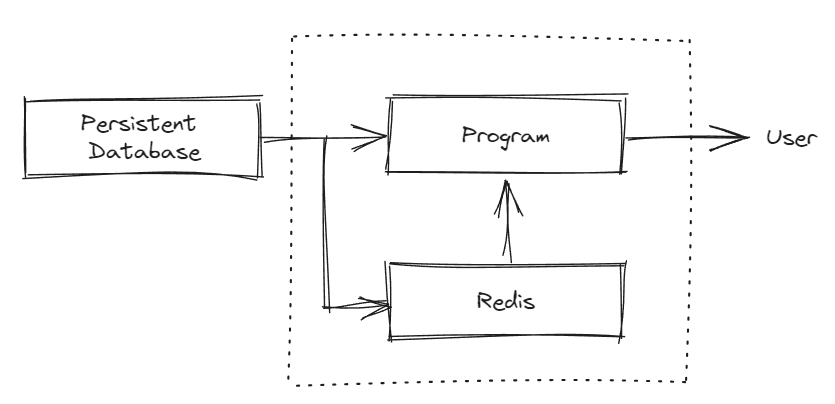
\includegraphics[width=0.8\textwidth]{chapters/part-3/figures/redis_architecture.png}
	\caption{A commonly seen architecture of implementing Redis.} \label{ch:database:redisarchitecture}
\end{figure}

Other than replica of database for reading, the following gives a list use cases where Redis may be helpful:
\begin{itemize}
	\item Data caching
	\item Message brokering
	\item Distributed locking
	\item Real-time data streaming, processing and analyzing
\end{itemize}

In addition to Redis CLI which a user can use to interact with Redis from the console, Redis also supports the following main languages. The program in these languages can connect to Redis via the Redis client.
\begin{itemize}
\item Python
\item C\# / .NET
\item Node.js
\item Java
\item Go
\end{itemize}
More information is given at \cite{redis2024client}.






\chapter{Virtualization and Containerization} \label{ch:vac}

Virtualization and containerization are widely appreciated technologies for distributing multiple instances of applications on single or multiple physical servers. The primary objective of these technologies is to enhance resource utilization efficiency while ensuring isolation between applications.

\section{Introduction}

One of the major differences between a server and a PC is that the former is usually shared among multiple users or applications at the same time. Though working on the same machine, a user would usually want a private working environment not interrupted by other users. In other words, a user would want to ``virtually'' work on an independent machine with his own CPU, RAM, I/O, OS, drivers and storage, despite that the actual hardware is shared with others. This can be achieved through \textit{virtualization}, which enables running multiple operating systems on a single physical server in an uninterrupted and logically separated manner. The virtually independent computer of such kind is often called a \textit{virtual machine} (VM).

Deploying a new VM generally consumes a considerably large amount of time and resources. This is because different VMs on the same server are separated at the OS level, with each VM requiring its own OS installation. Consider a scenario where there are hundreds of small applications (microservices), each requiring a similar but separate environment. Launching VMs for each and every of them is resource-intensive and can become an unnecessary waste of resource when these applications could have shared the same OS kernel and operated within their own isolated workspace.

In the above scenario, a more efficient approach is to deploy a single VM and place each application in a ``container'' with its own customized drivers and configurations. A container is similar to a VM in the sense that it provides a degree of isolation from others, but it is typically ``lighter'' than a VM because it doesn't need to virtualize or duplicate the whole OS as VMs do. This makes containers cheaper to launch and manage.

The technology used to deploy and manage containers is known as \textit{containerization}. A container contains all the configuration and requirement information of an application. Running a container on different platforms would consistently generate the same expected result. This has made the sharing and rapid deployment of containers remarkably easy and convenient. The similarities and differences of personal PCs, VMs, and container applications are summarized in Fig. \ref{ch:vac:fig:pcvmcontainersructure}.

\begin{figure}
	\centering
	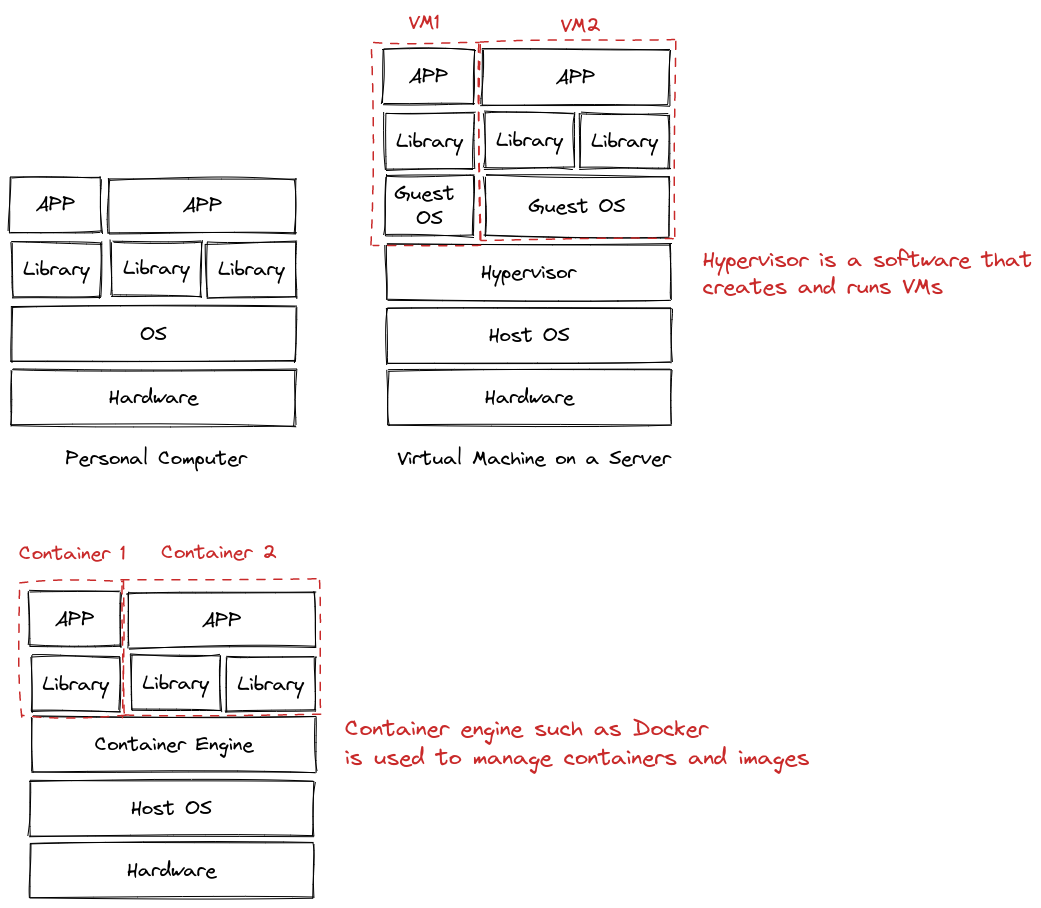
\includegraphics[width=350pt]{chapters/part-3/figures/pcvmcontainerstructure.png}
	\caption{System architectures of PC, VM and container.} \label{ch:vac:fig:pcvmcontainersructure}
\end{figure}

As an analogy, think of running an APP as cooking a dish. The hardware corresponds with the physical resources in the kitchen such as the cooktop and gas. The OS corresponds with the cook. The OS requires drivers and libraries to run the APP correctly. The drivers and libraries correspond with the specific skills or cookers for the dish. Finally, the APP is corresponding with the expected dish.

In the most simple configuration, a dedicated machine is used to run an APP. This is like constructing a dedicated kitchen and hiring a dedicated cook for each dish. The cook is trained to master all necessary skills required for that specific dish. This is shown in Fig. \ref{ch:vac:fig:acookinakitchen}.
\begin{figure}[htbp]
	\centering
	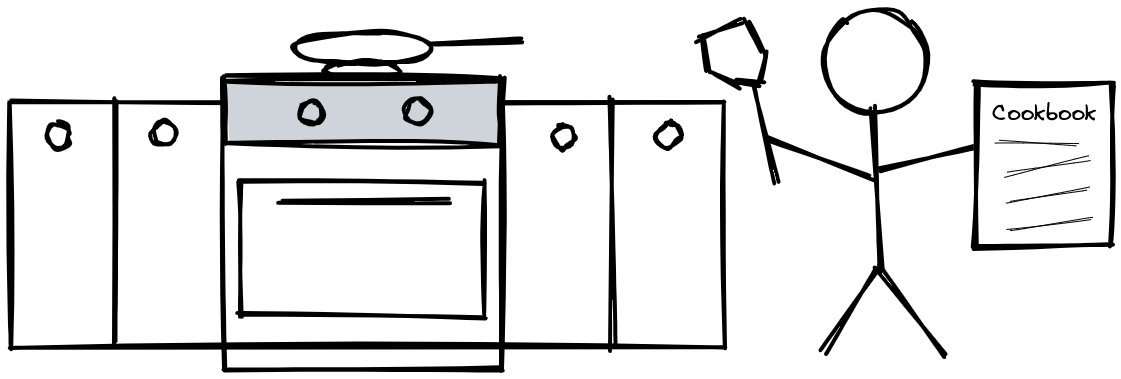
\includegraphics[width=300pt]{chapters/part-3/figures/acookinakitchen.png}
	\caption{PC implementation: a cook in a kitchen.} \label{ch:vac:fig:acookinakitchen}
\end{figure}

In a VM implementation, a large and capable kitchen is setup in advance as shown in Fig. \ref{ch:vac:fig:manycooksinakitchen}. For each dish, a cook is hired. Each cook is trained with the skills necessary for his assigned dish. All cooks share the same kitchen. This implementation is more efficient than Fig. \ref{ch:vac:fig:acookinakitchen}, as there is no need to scale up the kitchen for a new dish. By sharing the resources among the cooks, the kitchen can be utilized more efficiently.
\begin{figure}[htbp]
	\centering 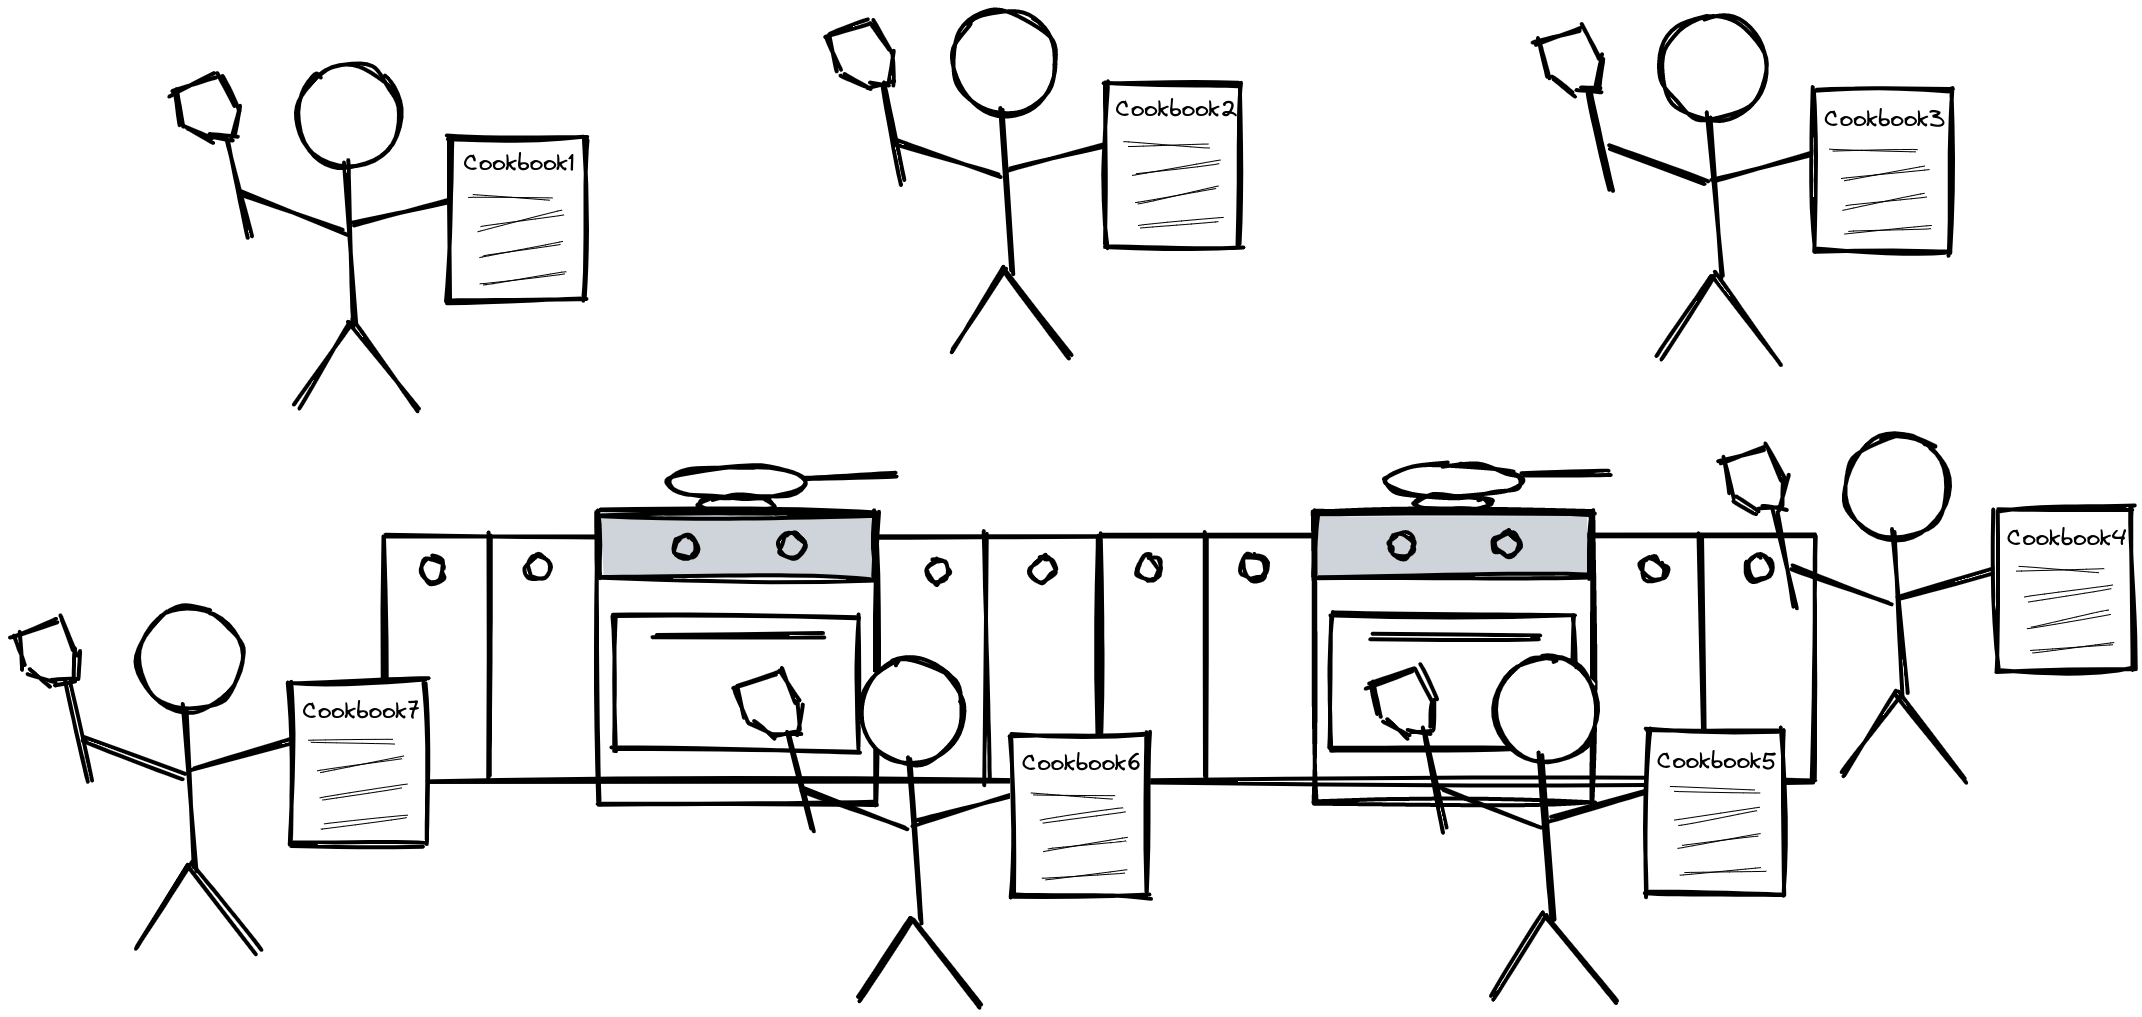
\includegraphics[width=350pt]{chapters/part-3/figures/manycooksinakitchen.png}
	\caption{VM implementation: many cooks in a kitchen, each with a different cookbook.} \label{ch:vac:fig:manycooksinakitchen}
\end{figure}

While Fig. \ref{ch:vac:fig:manycooksinakitchen} might be a popular practice in many restaurants, it is still too costly to hire a new cook for each dish. In a containerization implementation, a cook usually handles a category of dishes, as shown in Fig. \ref{ch:vac:fig:multitaskcook}. Of course, each dish will stay in its own fry-pan in an isolated way. For each dish, its recipe is provided that gives all information required to prepare the dish consistently. As long as the cook is good at multi-tasking and has the basic skill sets for general dishes, Fig. \ref{ch:vac:fig:multitaskcook} is usually a more efficient implementation than Figs. \ref{ch:vac:fig:acookinakitchen} and \ref{ch:vac:fig:manycooksinakitchen}.

\begin{figure}[htbp]
	\centering
	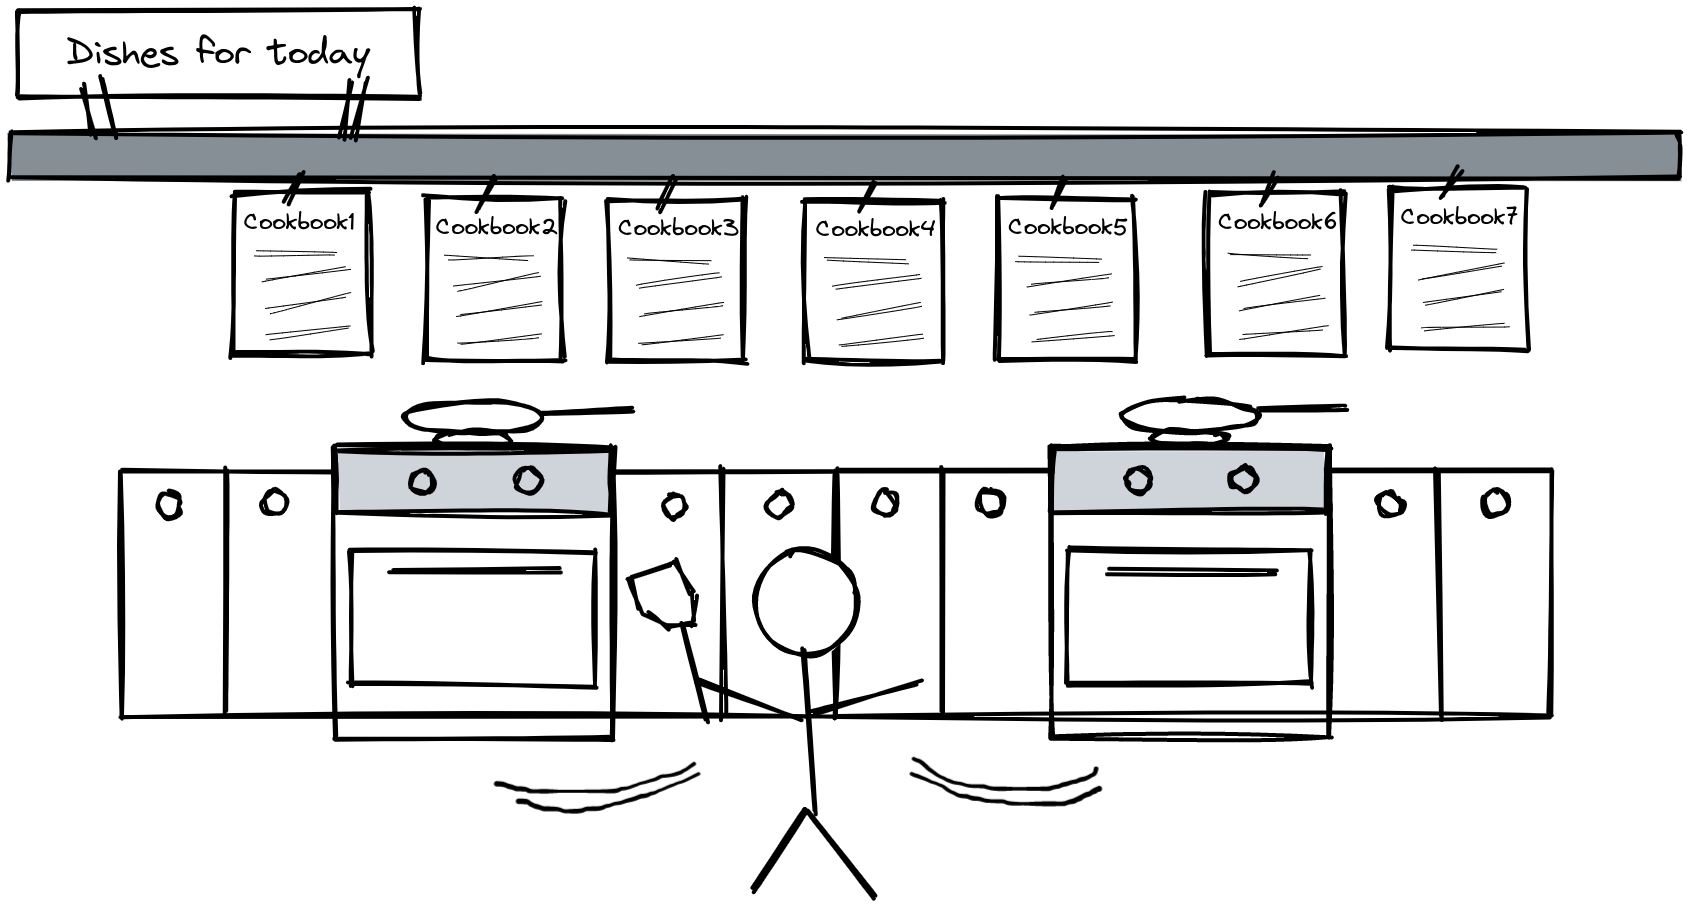
\includegraphics[width=350pt]{chapters/part-3/figures/multitaskcook.png}
	\caption{Container implementation: one cook in a kitchen, handling multiple dishes, each has a cookbook and stays in its own pan.} \label{ch:vac:fig:multitaskcook}
\end{figure}

Just like a recipe guaranteeing the consistency of dishes, in containerization, an ``image'' guarantees the consistent behavior of container instances. An image is basically a collection of prerequisites and configurations to start a container efficiently and consistently. Images can be shared among machines to replicate the containers even if the machines adopt different underlying infrastructures such as hardware and OS.

\section{Virtualization and Containerization}

Virtualization and containerization have been studied for decades. This section gives a brief introduction to both technologies.

\subsection{Virtualization}

In a conventional data center, multiple physical servers are deployed, and each server has a single associated application. Servers may share the same LAN and network-attached storage (NAS) for data exchanging. A big issue of this implementation is the utilization efficiency of the servers and the unevenly distributed loads: some of the servers may not be utilized efficiently, while others may be overwhelmed. To deploy a new application, a new server must be purchased, which can take months of time. With more and more servers, the management and IT cost may grow exponentially.

To solve this problem, we need a systematical and automated way of integrating the resources in a data center and re-distributed them to the applications in an efficient manner. Virtualization is one of the most important technology used in this framework. Virtualization is essentially about running a system on a ``virtualized machine'', where by saying ``virtualized'' we mean that the machine is not a physical machine, but a virtual execution environment that is emulated and managed by a special software running on the actual machine known as the ``hypervisor''. The setup should be transparent to the applications in the sense that the applications perform the same way as if it were running on a dedicated physical machine.

Depending on the items to be virtualized, virtualization can be divided into the following categories.
\begin{itemize}
  \item Virtualization of equipment, mainly network resources and storages. This results in virtual local area network (VLAN), virtual private network (VPN), NAS and storage area network (SAN).
  \item Virtualization of operating systems. This results in the well-known VM and virtual desktop.
  \item Virtualization of application running environments. An example is Java virtual machine (JVM) that allows Java to generate consistent result while running on different machines.
\end{itemize}

There are different virtualization architectures. Commonly seen components shared by different architectures often include
\begin{itemize}
	\item Host OS. The OS that resides on the physical machine, on which virtualization tools run.
	\item Virtual Machine Monitor (VMM), also known as the hypervisor. This is a software that runs on the host OS, managing all the guest OSs, providing them interface to the host OS and the hardware.
	\item VM, the system that runs in an virtualized isolated environment.
\end{itemize}
Host OS, VMM and VM relationship is shown in Fig. \ref{ch:vac:fig:acookinakitchen}.

Different virtualization techniques are used in different types of VMMs. They can be widely divided into the following categories.
\begin{itemize}
	\item Full virtualization. The VMM virtualizes everything including the hardware. The guest OS can run on the VM without modification or adaptation, just like running on any other machine.
	\item Para-virtualization. The VMM does not virtualize hardware. The guest OS is modified to certain extent to suit the VMM of this type.
	\item Hardware-assisted virtualization. The processor of the system is specifically designed to provide certain VM functions. These functions, after passing through VMM, are directed and executed on the hadrware, thus enhancing system performance.
\end{itemize}

VMM is able to virtualize hardware resources such as CPU, memory and I/O. For the virtualization of CPU, the key is to virtualize privileged instructions (a set of instructions that can only be executed by software running in privileged mode, usually the OS) for the guest OS, so that the guest OS would think it is directly talking to a CPU. This is challenging because guest OS usually does not possess the privilege due to the VM architecture. If the requests of the guest OS contain privileged instructions, the CPU will deny the request. When that happens, an exception will be raised to the VMM which will take care of the privileged instructions sequentially. Since hypervisor runs in privileged mode, it can execute those instructions.

For the virtualization of memory, VMM uses shadow page table to assign memory pages to different VMs. The maximum memory allocated to a VM can change dynamically.

For the virtualization of I/O, the development trend is that I/O operations will be less and less rely on software and OS, and more and more on hardware. The VMM directly maps the I/O hardware interface to the VMs.

\begin{shortbox}
	\Boxhead{Hypervisor VS Host OS, Who is the Boss?}
	Both the hypervisor and the host OS can run in privilege mode (also known as ``Ring 0'' in x86 architecture). However, notice that at one time there can be only one boss, i.e., there can be only one entity that runs in Ring 0 at the same time.
	
	Depending on the type of the hypervisor configuration, this entity can be either the hypervisor or the host OS. In a type 1 hypervisor configuration, the hypervisor itself runs in Ring 0 and manages all hardware resources directly. In a type 2 hypervisor configuration, the host OS runs in Ring 0, and the hypervisor runs in a lower privileged ring.
\end{shortbox}

\subsection{Containerization}

Containerization is an alternative virtualization approach to VM that can also virtualize independent workspaces for applications. Comparing with VM, containers are often lighter, hence more efficient for massive microservices deployment. Depending on the context, the term ``container'' may refer to one or more of the following 3 concepts: container runtime, container engine, and container orchestration.

Container runtime refers to the backend software that actually executes the containers. Examples of widely used container runtimes are ``containerd'', ``runc'' and ``cri-o''. 

It is often inconvenient for users to talk to container runtimes directly. Container engine is the interface for a user or software to manage images and containers. Examples of container engines include ``docker'' and ``podman''. 

Finally, container orchestration is the software that strategically deploy, monitor, restart, and terminate the containers on servers. It can scale up and down the number of containers based on the demanding, and balance the API calls each container receives. Container orchestration is very useful in production environment of large-scale services. One of the most widely used container orchestrations is ``kubernetes''.

Notice that though container runtime is always a must-have, container engine and container orchestration are not.

\section{Docker Container Basics} \label{ch:vac:sec:dc}

This section introduces docker. Notice that though being famous for docker container engine, docker as a company or community provides many revolutionary container related tools and services that go far beyond a container engine brand. Many tools and technologies of docker are used in container runtimes and container engines of other brands.

This section focuses mostly on the introduction of docker container engine.

\subsection{Docker Engine VS Alternatives}

Docker engine is the most popular container engine available on the market as of 2023, and it is free of charge for open-source, personal and small business usage. More details of docker can be found at \textit{https://docs.docker.com/}.

But does that mean docker engine is the absolutely best and perfect container engine solution?

Docker has surely revolutionized how we use containerization technology in software development and deployment, and it has been one of the most popular and beloved container engine solutions. However, it is worth mentioning that docker engine is not the only available container engine. For example, as explained earlier podman is an alternative to docker. It supports the same interface as docker in its CLI (as if podman were an alias), and claims to have better performance and security. As a matter of fact, RHEL already started the transition from docker to podman from RHEL 8. Nowadays, installing docker on the latest versions of RHEL is possible but tedious. On the other hand, installation of podman on RHEL, if it had not been pre-installed, can be done simply by
\begin{lstlisting}
$ sudo dnf install podman
\end{lstlisting}
Kubernetes, a famous container orchestration, is also dropping docker support according to their statement ``docker support in the kubernetes is now deprecated and will be removed in a future release''. Some may even argue that ``containers are alive, but the role that docker plays is shrinking''. Many open-source initiatives such as podman are gaining popularity.

Docker has some disadvantages indeed. For one thing, docker uses docker server (docker daemon), a single piece of software running in the backend of the system, to support all the services. This creates a single-point-of-failure in the system. Docker requires root privileges, and it starts a container on behalf of the root user. This means that the program running inside the container and the users in the docker group can potentially bypass the OS access control and gain root access, which introduces security risk. These shortages are to some extent addressed by other container engines such as podman which is daemon-less and does not necessarily need to run on root user's behalf.

This is not to say that Docker is falling behind as a whole. Some key techniques that docker introduced are widely used in all different types and brands of container runtimes and engines. It is just that people do not like some of the features of docker engine, and alternative tools are being developed to fix these problems, the latter of which starting drawing more and more attention. Docker still enjoys widespread usage and support due to its massive community, wealth of online resources, and extensive compatibility with numerous tools and platforms. Nevertheless, for demonstration purpose, for the remaining sections docker is used throughout this notebook. Since podman provides the same interface, it is probable that podman can be used likewise to replicate all the results.

As of 2023, docker is still the dominating container market engine, with a market share of over $80\%$.

\subsection{Docker Installation}

To install docker on a Linux machine, go to \textit{https://www.docker.com/} to look for the instruction. The installation steps differ depending on the host machine. As explained earlier, RHEL uses podman as its recommended container engine, and podman comes with RHEL installation. 

In this section, consider installing docker engine on Ubuntu. Some of the key steps are summarized as follows. Remove existing docker engine, if any.
\begin{lstlisting}
$ sudo apt-get remove docker docker-engine docker.io
$ sudo apt-get remove containerd runc
\end{lstlisting}
Add docker's official GPG key and set up the repository.
\begin{lstlisting}
$ sudo apt-get update
$ sudo apt-get install ca-certificates curl gnupg lsb-release
$ sudo mkdir -p /etc/apt/keyrings
$ curl -fsSL https://download.docker.com/linux/ubuntu/gpg | sudo gpg --dearmor -o /etc/apt/keyrings/docker.gpg
$ echo \
  "deb [arch=$(dpkg --print-architecture) signed-by=/etc/apt/keyrings/docker.gpg] https://download.docker.com/linux/ubuntu \
  $(lsb_release -cs) stable" | sudo tee /etc/apt/sources.list.d/docker.list > /dev/null
\end{lstlisting}
Install docker.
\begin{lstlisting}
$ sudo apt-get update
$ sudo apt-get install docker-ce docker-ce-cli containerd.io docker-compose-plugin
\end{lstlisting}
where notice that \verb|docker-compose| is a toolkit to manage containers using CLI. It is a handy tool in the testing environment.

To test whether docker is installed correctly, run
\begin{lstlisting}
$ sudo docker run hello-world
\end{lstlisting}
and if everything is done correctly, a message started with ``Hello from Docker!'' will be displayed in the console, together with a brief introduction to how docker works.

Notice that to use docker commands, sudo privilege is required. To avoid typing \verb|sudo| each time running a docker command, add the user to the docker group as follows. In the rest of the section, \verb|sudo| is neglected for docker commands.
\begin{lstlisting}
$ sudo usermod <user name> -aG docker
\end{lstlisting}

Docker installs at least two piece of software on the machine, namely docker CLI and docker server. The CLI is the interface to the user, and the server the daemon. Docker runs natively on Linux OS. If docker is installed on non-Linux system such as Windows or macOS, ``docker desktop'' is used which includes a Linux VM to host the docker daemon and run Linux-based containers.

\subsection{Docker Container Management}

\vspace{0.1in}
\noindent \textbf{Launch}
\vspace{0.1in}

To create and run a container from an image, simply use
\begin{lstlisting}
$ docker run <configuration> <image>
\end{lstlisting}
Docker will search the local and remote repositories for the image, download the image if necessary, and start a container from that image. By default, \verb|docker run| starts a container in attached mode (frontend mode) unless flag \verb|-d| is used. After successful execution and completion of all the tasks, the container will enter ``Exited'' status. 

For example, consider running a container of \textit{alpine} using the command below. A screen shot is given in Fig. \ref{ch:vac:fig:dockerrunexp}.
\begin{lstlisting}
$ docker run -it --name test-alpine alpine
\end{lstlisting}
where \verb|-i| stands for ``interactive'', which keeps the container's standard input (i.e., the console in this example) open so that the user can actively interact with the container. Option \verb|-t| allocates a pseudo-TTY to the container. TTY stands for ``TeleTYpewriter'', which enforces the I/O of the container to follow the typical terminal format and allows the user to interact with the container like a traditional terminal, hence making the interactive interface a bit more user-friendly. Flags \verb|-it| are often used when running a container in attached mode. Finally, \verb|--name| assigns a name to the container. Without an assigned name, docker will assign a random name to the container.
\begin{figure}[!htb]
	\centering
	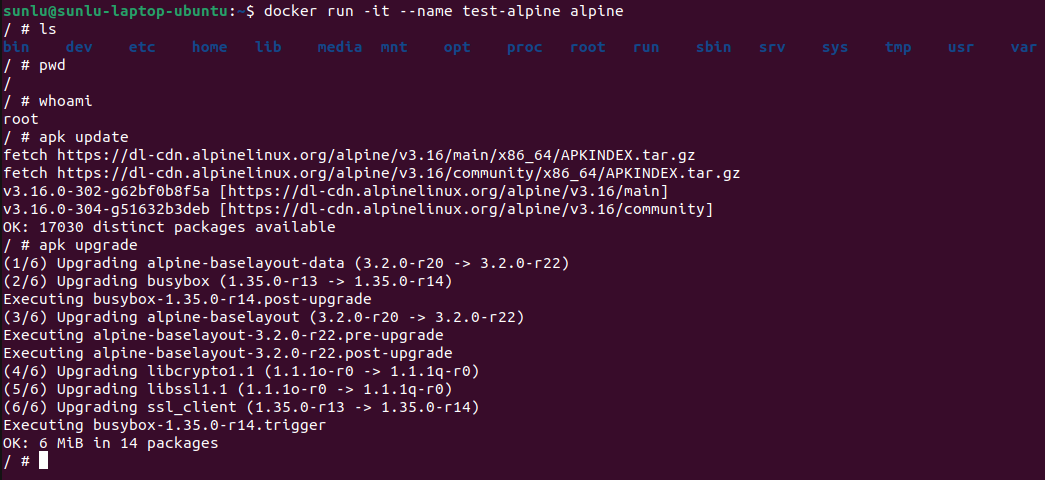
\includegraphics[width=350pt]{chapters/part-3/figures/dockerrunexp.png}
	\caption{An example of running \textit{apline} container, with interactive TTY and name \textit{test-apline}.} \label{ch:vac:fig:dockerrunexp}
\end{figure}

It can be seen from Fig. \ref{ch:vac:fig:dockerrunexp} that once the container is started, the user can interact with the container via shell and perform actions such as listing items in the current directory in the container. This is because the container is running in attached mode, and flags \verb|-it| map the the containers input and output with the console.

While keeping the container running, open another terminal and use \verb|docker container ls| to check the status of the container. More about \verb|docker container ls| are introduced later. The container \verb|test-alpine| shall appear in the list, as shown in Fig. \ref{ch:vac:fig:dockerrunexppart2}.
\begin{figure}[!htb]
	\centering
	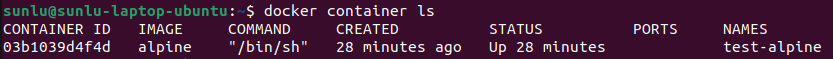
\includegraphics[width=250pt]{chapters/part-3/figures/dockerrunexppart2.png}
	\caption{List the running container \textit{test-apline}.} \label{ch:vac:fig:dockerrunexppart2}
\end{figure}
After exiting from Fig. \ref{ch:vac:fig:dockerrunexp} (by using \verb|exit| in \textit{alpine}), the container will transfer its status from ``running'' to ``exited'', as shown in Fig. \ref{ch:vac:fig:dockerrunexppart3}.
\begin{figure}[!htb]
	\centering
	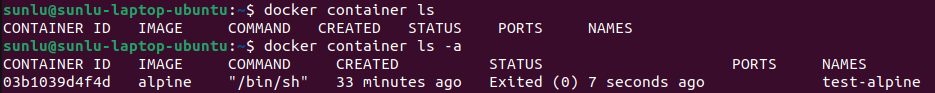
\includegraphics[width=250pt]{chapters/part-3/figures/dockerrunexppart3.png}
	\caption{List the exited container \textit{test-apline}.} \label{ch:vac:fig:dockerrunexppart3}
\end{figure}

Functional wise, \verb|docker run| executes two commands behind the screen, namely \verb|docker create| and \verb|docker start|, where \verb|docker create| creates a container and \verb|docker start| starts the container by executing the startup script defined in the image. These two commands can be used separately. For example, to start an exited container, use
\begin{lstlisting}
$ docker start <container>
\end{lstlisting}

\begin{shortbox}
\Boxhead{Differences between \texttt{docker run} and \texttt{docker start}}

Do note the fundamental differences between \verb|docker run| and \verb|docker start|. First of all, \verb|docker run| starts a container from an image and it always creates a new container, whereas \verb|docker start| starts an existing but exit container. Secondly, \verb|docker run| runs a container in attached mode by default unless \verb|-d| flag is used, while in contrast \verb|docker start| runs a container in detached (backend) mode by default unless \verb|-a| is used. 
\end{shortbox}

An example of using \verb|docker run| with \verb|-d| flag to start a container in detached mode is given below.
\begin{lstlisting}
$ docker run -d --name test-background-alpine alpine
\end{lstlisting}
By changing \verb|-it| to \verb|-d|, the container runs in the backend silently. The status of the container, after executing the above command, will stay running and can be displayed by \verb|docker container ls|.

Commonly used commands regarding launching a container are given in Table \ref{ch:vac:tab:launchcontainer}.

\begin{table}[!htb]
	\centering \caption{Commonly used docker commands to launch a container.}\label{ch:vac:tab:launchcontainer}
	\begin{tabularx}{\textwidth}{llX}
		\hline
		Command & Flag & Description \\ \hline
		\verb|docker run| & --- & Launch a container from an image in attached mode by default. If the image cannot be found locally, it downloads the image from the remote repository automatically. \\
        \verb|docker start| & --- & Start an existing but exit container in detached mode by default. \\
        \verb|docker run| & \verb|-i| & Keep the standard input of the container open when launching the container. \\ 
        \verb|docker run| & \verb|-d| & Launch the container in the backend and keep it running. \\ 
        \verb|docker run| & \verb|--rm| & Automatically remove the container when exiting. The removed container will not be listed in \verb|docker container ls -a|. This is usually used with temporary containers during debugging. \\ 
        \verb|docker run| & \verb|-t| & Allocate a pseudo-TTY. The flag usually comes with the flags \verb|-i| or \verb|-d|, to form \verb|-it| or \verb|-dt|. \\ 
        \verb|docker run| & \verb|--restart| & Enforce restart of the container upon exiting. This is usually used on containers running in the backend. Commonly used restart configurations include \verb|--restart no| (do not restart), \verb|--restart on-failure[:<max retries>]| (restart if exits with an error flag), \verb|--restart always| (always restart when exists). \\ 
        \verb|docker run| & \verb|--name| & Assign a name to the container. \\
		\hline
	\end{tabularx}
\end{table}

It is worth mentioning that file system snapshot and startup commands are defined inside an image. See Section \ref{ch:vac:sec:di} for more details. When a container starts, the file system snapshot is pasted to the container file system, and the startup commands executed. It is possible to overwrite the startup commands when starting a container, simply by amending the revised startup commands to the image name as follows.
\begin{lstlisting}
$ docker run <image> <revised command>
\end{lstlisting}
where \verb|<revised command>| must be defined in the image, or otherwise an error will be raised.

\vspace{0.1in}
\noindent \textbf{Interaction}
\vspace{0.1in}

For a container running in the backend, use \verb|docker exec| to execute a shell command in that container as follows.
\begin{lstlisting}
$ docker exec <container> <command>
\end{lstlisting}
To enable the TTY shell of a container running in the backend, use
\begin{lstlisting}
$ docker exec -it <container> <command>
\end{lstlisting}
If \verb|<command>| is replaced by the shell name used in the container, this would open the terminal of the container. Notice that the shell used by the application running inside the container may differ from the one used in the host machine. In the case of an \textit{alpine} image based container, \verb|ash| is the default shell. For a \textit{ubuntu} image based container, \verb|bash| is often used. To exit from the TTY shell while keep the container running in the backend, use shortcut key \verb|Ctrl+p+q|. An alternative way to interact with containers running in the backend is to use
\begin{lstlisting}
$ docker attach <container>
\end{lstlisting}
to attach local standard input, output, and error streams to a running container. Similar with the previously introduced \texttt{docker exec -it} command, \texttt{docker attach} also starts the shell of the application running in the container. Use \verb|Ctrl-C| to quite the shell.

\vspace{0.1in}
\noindent \textbf{Stop and Removal}
\vspace{0.1in}

To stop, kill or restart a container running in the backend, use
\begin{lstlisting}
$ docker stop <container>
$ docker kill <container>
$ docker restart <container>
\end{lstlisting}
respectively. The difference between \verb|docker stop| and \verb|docker kill| concerns with how the OS manages process. When \verb|docker stop| is used, a  \verb|SIGTERM| signal is sent to the main process that the container runs. The container still has a little bit of time (maximum $10$ seconds) to terminate the job and clean up. When \verb|docker kill| is used, \verb|SIGKILL| signal is sent to the process, and the process is terminated immediately. When a container is stopped, it enters exited status.

To remove an exited container, use
\begin{lstlisting}
$ docker (container) rm <container>
\end{lstlisting}
where \verb|container| can be neglected. Alternatively, use
\begin{lstlisting}
$ docker container prune
\end{lstlisting}
to remove all exited containers. Notice that there is a more powerful command
\begin{lstlisting}
$ docker system prune
\end{lstlisting}
which removes not only exited containers but also unused network configurations, dangling images and cache.

\vspace{0.1in}
\noindent \textbf{Rename}
\vspace{0.1in}

To rename a container (without changing its container ID or anything else), use
\begin{lstlisting}
$ docker rename <container-old-name> <container-new-name>
\end{lstlisting}

\vspace{0.1in}
\noindent \textbf{Monitoring}
\vspace{0.1in}

Use
\begin{lstlisting}
$ docker container ls
\end{lstlisting}
to check the list of running containers, and
\begin{lstlisting}
$ docker container ls -a
\end{lstlisting}
the list of all containers, running or exited. Alternatively, \verb|docker ps|, \verb|docker ps -a| can also be used to list down containers just like \verb|docker container ls|, \verb|docker container ls -a|.

To check the processes that is running in the container, use
\begin{lstlisting}
$ docker top <container>
\end{lstlisting}

To quickly check container status including resource consumption (CPU, memory usage, etc.), use
\begin{lstlisting}
$ docker stats [<container>]
\end{lstlisting}
where the user can choose to list down all containers or a specified container. To show more detailed information of a container, including its status, gateway, IP address, etc., use
\begin{lstlisting}
$ docker inspect <container>
\end{lstlisting}
Finally, to check the logs of a container such as its standard output or error message, use
\begin{lstlisting}
$ docker logs <container>
\end{lstlisting}

\vspace{0.1in}
\noindent \textbf{File Exchange with Host Machine}
\vspace{0.1in}

There are multiple ways and protocols to access the files in a container, depending on the I/O setup of the container. For a container running locally, \verb|docker cp| can be used for file transfer between the container and the host machine as follows. From container to host machine:
\begin{lstlisting}
$ docker cp <container>:<source> <destination>
\end{lstlisting}
and from host machine to container:
\begin{lstlisting}
$ docker cp <source> <container>:<destination>
\end{lstlisting}
where \verb|<source>| and \verb|<destination>| refer to the path to the source and destination, respectively, located in the host machine or the container.

\vspace{0.1in}
\noindent \textbf{Commit}
\vspace{0.1in}

A container is usually generated from an image. It is also possible to do vise versa, i.e., packaging a container into an image. Notice that this is generally not recommended. Images shall be created mostly from Dockerfile, as will be introduced in Section \ref{ch:vac:sec:di}.

To create an image from a container, use
\begin{lstlisting}
$ docker commit <container> <image>
\end{lstlisting}
or
\begin{lstlisting}
$ docker commit -c 'CMD ["<startup command>"]' <container> <image>
\end{lstlisting}
where \verb|docker commit| command saves the container's file changes or settings into a new image, which allows easier populating containers or debugging in a later stage. Notice that \verb|docker commit| does not save everything of the container into the image, and it is not the only way an image is created.

\vspace{0.1in}
\noindent \textbf{Ports Publishing}
\vspace{0.1in}

By default, containers do not expose any ports to the outside world. A container can be accessed only from its host machine using APIs provided by docker, such as \verb|docker cp| to transfer files and \verb|docker exec| to execute commands, but not network protocols. The user can allow public access from the internet by publishing the ports of the container using
\begin{lstlisting}
$ docker run -p <host machine port>:<container port> <image>
\end{lstlisting}
when starting a container. To publish multiple ports, use multiple \verb|-p| flags in a command.

More about containerized application connectivity to the internet, to the host machine and to other containerized applications are introduced in later sections.

\subsection{An Example: Deploy a Containerized Application}

An example of setting up a web server in containers from scratch is given in this section. For simplicity, everything happens on a single physical server. Only one container is used and the load balancer and the shared services are not included in the example.

As a first step, create a container from the official \textit{nginx} image as follows. Notice that it is also possible to create a container from \textit{apline}, and install \textit{nginx} on \textit{apline}.
\begin{lstlisting}
$ docker run -dt --name simple-web nginx
\end{lstlisting}

Next, create the configuration file for \textit{nginx}, and also the \textit{html} files to be used as the static web page. For convenience, the files are created and edited in the host machine, then copied to the container. The following \textit{default.conf} and \textit{index.html} have been created, respectively. The configuration file \textit{default.conf} is given below.
\begin{lstlisting}
server {
	listen 80 default_server;
	listen [::]:80 default_server;
	root /var/www/html/;
}
\end{lstlisting}
The \textit{html} file \textit{index.html} is given below.
\begin{lstlisting}
<html>
	<body>
		<h1>Hello World!</h1>
	</body>
</html>
\end{lstlisting}
Use \verb|docker copy| to copy the two files to the designed locations in the container as follows. Notice that for read-only configuration files, unlike what we are doing now, a good practice is to build them into the read-only image layers. Keep in mind that this serves only as an demonstrative example. More about images are given in later sections.
\begin{lstlisting}
$ docker exec simple-web mkdir -p /var/www/html
$ docker cp default.conf simple-web:/etc/nginx/conf.d/default.conf
$ docker cp index.html simple-web:/var/www/html/index.html
\end{lstlisting}
where \verb|mkdir -p| creates the directories along the given path, if not exist. Notice that the file name in the destination can be ignored if it is the same with the source, i.e., the copy commands can be replaced by
\begin{lstlisting}
$ docker cp default.conf simple-web:/etc/nginx/conf.d/
$ docker cp index.html simple-web:/var/www/html/
\end{lstlisting}

Change the ownership of the \textit{html} file as follows, so that the current user \textit{nginx} is able to access that file.
\begin{lstlisting}
$ docker exec simple-web chown -R nginx:nginx /var/www/html
\end{lstlisting}

Finally, reload and configuration file and restart the web server as follows.
\begin{lstlisting}
$ docker exec simple-web nginx -s reload
\end{lstlisting}

To test the web server running inside the container, obtain the IP address of the container using
\begin{lstlisting}
$ docker inspect simple-web | grep IPAddress
\end{lstlisting}
and open a browser to key in the obtained IP address. If everything is done correctly, the browser should try to access port 80 of the container, and the ``Hello World!'' web page shall show up.

For easy sharing and populating of the container, commit the container into a new image using \verb|docker commit| as follows. The new image can be used to populate the web server, just like ``web01'' container given below.
\begin{lstlisting}
$ docker commit simple-web simple-web-image
$ docker run -dt --name web01 -p 80:80 simple-web-image
\end{lstlisting}
where \verb|-p <host machine port>:<container port>| is used to map ports. Notice that different from the previous container ``\textit{simple-web}'', the new container ``\textit{web01}'' IP address port 80 is mapped with the port 80 of the host machine. Therefore, the web page hosted in ``\textit{web01}'' can be accessed not only by the host machine, but also by other machines in the same network with the host machine.

\section{Docker Volume and Bind Mount} \label{ch:vac:subsec:dockervolume}

When a container is running, files inside it can be accessed or copied bidirectionally using the \verb|docker cp| command. However, all data created or modified during the container's life cycle resides in the container's writable layer. More about the concept of layers are introduced in later section. If the container is removed, all data stored in its writable layer is also lost.

To ensure data persistence, it is best practice to use Docker volumes or bind mounts. Both methods link storage on the host machine to the container, allowing data to persist even if the container is removed.
\begin{itemize}
  \item Docker volumes are fully managed by Docker. The user does not directly interact with the storage on the host machine. There are two types of docker volumes, the anonymous volume and the named volume.
  \item Bind mounts, on the other hand, allow the user to specify and manage the storage location on the host machine, providing direct control over the data.
\end{itemize}

In addition to data persistence, named docker volumes and bind mount can also play as a hub to shared data among multiple containers, which facilitates data exchange and allows containers to work on the same dataset. 

\subsection{Volume}

In this section, we only consider named docker volume.

To create a docker volume, use
\begin{lstlisting}
$ docker volume create <volume>
\end{lstlisting}
Notice that docker volume is fully managed by docker. The user cannot, and does not need to specify where the data should be stored in the host machine.

To list down volumes and to inspect a volume, use
\begin{lstlisting}
$ docker volume ls
$ docker volume inspect <volume>
\end{lstlisting}
respectively. Notice that when using \verb|docker volume inspect|, docker gives the mount point of the volume. However, the mount point is often a place in a virtual machine that docker creates, therefore, difficult to locate in the host machine. Like said earlier, the user should not access the data of a volume from the host machine directly.

Finally to remove specific an unused volume(s) or all unused volumes, use
\begin{lstlisting}
$ docker volume rm <volume>
$ docker volume prune
\end{lstlisting}
respectively. When a volume is removed, all the data is lost.

When starting a container from an image, volumes can be mapped with the internal storage inside the container by using \verb|-v| flag as follows
\begin{lstlisting}
$ docker run -v <volume>:<container path>[:ro] <image>
\end{lstlisting}
which should mount \verb|<volumn>| to \verb|<container internal path>|. If \verb|<volumn>| is not created before hand, docker will create a docker volumn with the name. The optional \verb|:ro| can be used if it is a read-only volume, i.e., the container can only read from the volume but not write back to the volume. This can become handy if the volume is shared by multiple containers and only one of them is allowed to writer to the volume while others being only the listener.

Notice that if not specifying the volume name when using flag \verb|-v|, i.e.,
\begin{lstlisting}
$ docker run -v <container-path> <image>
\end{lstlisting}
an anonymous volume will be created and used. Further more, if \verb|--rm| is used, when the container is stopped, the container together with the anonymous volume will be removed. A use case of anonymous volume is given in the later section.
 Anonymous volumes can also be set up in the Dockerfile.

\subsection{Bind Mount}

Bind mount works similarly as docker volume, except that the user controls the location on the host machine where the data is persisted. Recall
\begin{lstlisting}
$ docker run -v <volume>:<container-path>[:ro] <image>
\end{lstlisting}
which associate a named docker volume to the path in the container. Instead of \verb|<volume>|, specify the path in the host machine as follows
\begin{lstlisting}
$ docker run -v <host-machine-path>:<container-path>[:ro] <image>
\end{lstlisting}
in which case docker will persist and synchronize the data on the paths inside and outside the container. Quotation marks can be used \verb|"<host-machine-path>"| if there are spaces or special characters in the host machine path. Notice that the specified host machine path should be accessible by docker. Likewise, the optional \verb|:ro| can be used to prevent the container from overwriting the host machine.

Bind mount is often used in development stage where the developer wants to map application source code or data on his host machine into the container directly. When the application is ready for shipping, the consolidated source code and data should be built into the image. You cannot expect the end user to have a separate copy of the source code and data on his machine, and to use bind mount each time he starts the application. 

Following that spirit, a developer can create a ``utility container''. He can start a container in \verb|-it| mode, install everything he needs to develop an application in that container, and develop the application there. Using bind mount, all the code he writes will be mirrored to his host machine. With this approach, he does not need to install all the dependencies of the application in his host machine.

\subsection{Multiple Volumes}

It is possible to run a container with multiple \verb|-v| flags, each pointing to a different path in the container. Should there be any clashes, the rules with more specific path wins. For example, consider
\begin{lstlisting}
-v <volume or path 1>:/app -v <volume or path 2>:/app/data
\end{lstlisting} 
used together in a \verb|docker run| command. In this example, \verb|/app/data| will be mounted to \verb|<volume or path 2>| and everything else in \verb|/app| to \verb|<volume or path 1>|. 

Consider
\begin{lstlisting}
-v <volume or path 1>:/app -v /app/data
\end{lstlisting} 
which mount an anonymous volume to \verb|/app/data| to protect it from being overwritten by any content in \verb|<volume or path 1>|. This is a good use case of anonymous volume.

\section{Container Communication}

In practice, a containerized application needs to communicate with applications running outside the container to request services such as API calls. Commonly seen use cases are as follows.
\begin{itemize}
	\item Containerized application requests services from the Internet.
	\item Containerized application requests services from the host machine, for example, from a database deployed on the host machine.
	\item Containerized application requests services from other containerized applications.
\end{itemize}

With proper port mapping using \verb|-p|, the communication with the Internet is automatically enabled. Therefore, the focus of this section is mainly on data exchange and API calls between the container and the host machine or other containers.

\subsection{Communication with Host Machine}

The containerized application may request services from the host machine. In this case, the application code needs to be modified to enable communications with the host machine. An example is given below.

Consider a simple scenario where the containerized application needs to send a request to the host machine to trigger an API call of MongoDB. Notice that the MongoDB is installed on the host machine and not in the container.

If the application were running on the host machine instead of in a container, it can communicate with the MongoDB server using a connecting string that looks like the following
\begin{lstlisting}
'mongodb://localhost:27017/<database name>'	
\end{lstlisting}
and it should be part of the application code. However, it would not work if the same code is used in the containerized application. The code needs to be modified as follows.
\begin{lstlisting}
'mongodb://host.docker.internal:27017/<database name>'	
\end{lstlisting}
where \verb|host.docker.internal| is a recognized domain by docker that refers to the host machine. Docker translates the domain to the IP address of the host machine.

Notice that \verb|host.docker.internal| can be used to refer to the host machine not only with MongoDB requests, but also with other requests such as a general HTTP request.

\subsection{Communication with Other Containers}

Two containers running on the same machine can always talk to each other via the host machine. However, this may become inefficient in some applications. Therefore, we need to investigate on direct container-to-container communication.

As a basic solution, cross container communication can be done following the example given below. Notice that this is not a common practice in production environment as it is not robust and efficient.

Consider a simple scenario where there are two containers, one running the application and the other hosting a MongoDB. 

The container with MongoDB deployment is started as follows.
\begin{lstlisting}
$ docker run -d --name mongodb mongo 	
\end{lstlisting}
where \verb|mongo| is the official docker image for MongoDB on Docker Hub.

The IP address of the MongoDB container can be found using
\begin{lstlisting}
$ docker container inspect mongodb	
\end{lstlisting}
where \verb|mongodb| is the name of the container specified in the earlier command. In the result of the inspection, look for \verb|IPAddress| under \verb|NetworkSettings|.

Then in the application code, replace \verb|localhost| in the connecting string
\begin{lstlisting}
'mongodb://localhost:27017/<database name>'	
\end{lstlisting}
with the IP address of the container.

Notice that each time a container is deployed, its network settings are done by docker and they differ from machine to machine. Therefore, this basic approach only works temporarily in development environment and should not be used in the production environment.

As a more established approach to realize cross container communication, docker allows the user to create container networks. All containers in a container network have reserved IP addresses assigned by docker and they can talk to each other.

To create a container network, use
\begin{lstlisting}
$ docker network create <network name>
\end{lstlisting}
Then to associate an container with that container network, use \verb|--network| as follows
\begin{lstlisting}
& docker run --network <network name>	<image name>
\end{lstlisting}
If two containers are put under the same container network, they can talk to each other. 

Consider the earlier example. We can create a container network using
\begin{lstlisting}
$ docker network create my-network
\end{lstlisting}
and launch MongoDB as a containerized application in the container network using
\begin{lstlisting}
$ docker run -d --network my-network --name mongodb mongo
\end{lstlisting}
In the application code, use
\begin{lstlisting}
'mongodb://mongodb:27017/<database name>'	
\end{lstlisting}
as the connecting string, and launch it in the same container network. Docker will automatically resolve \verb|mongodb| as the correct container with that container name when the application sends out the outbound request.

Notice that when using container network for cross container communication, there is no need to do port match using \verb|-p|. Indeed, \verb|-p| is used only when the container needs to talk to the outside world through the host machine. Cross container communication as well as container to host machine communication happens inside the host machine, thus not requiring port mapping.

\section{Docker Image} \label{ch:vac:sec:di}

Images are used to create containers. An image performs like a blueprint that encapsulates all the necessary information needed to spawn a container. It includes initial configurations, requisite libraries, and other pertinent metadata. Docker images are highly portable and can be shared across various machines and platforms. This section delves deeper into the construction and functionality of docker images.

\subsection{Dockerfile Programming}

An image shall contain everything needed to create and initialize a container. This includes but not limited to:
\begin{itemize}
  \item Necessary steps to create a container
  \item Files to support the application
  \item Libraries, tools and dependencies
\end{itemize}
In addition, an image shall be designed and organized in such a way that it is portable, reusable and light, and can be used to easily populate large number of containers. For better inheritability, an image might be based on another existing image, which is called its parent image. An image with no parent, such as the official \textit{hello-world} image from docker bub, is called a base image.

The most common and flexible way to create a docker image is to build from Dockerfile. The Dockerfile is a text document that serves as the blueprint for constructing a docker image. Generally speaking, a Dockerfile follows the following flow:
\begin{enumerate}[(1)]
	\item Specify base image
	\item Add additional configurations
	\begin{itemize}
		\item Setup file system
		\item Install dependencies and other programs
		\item ...
	\end{itemize}
	\item Specify startup command
\end{enumerate}
A more detailed step-by-step guidance example is given later. The relationship between Dockerfile, image and container is illustrated in Fig. \ref{ch:vac:fig:dockerfiletoimage}. Notably, the Dockerfile itself isn't included within the resulting image.

\begin{figure}[!htb]
	\centering
	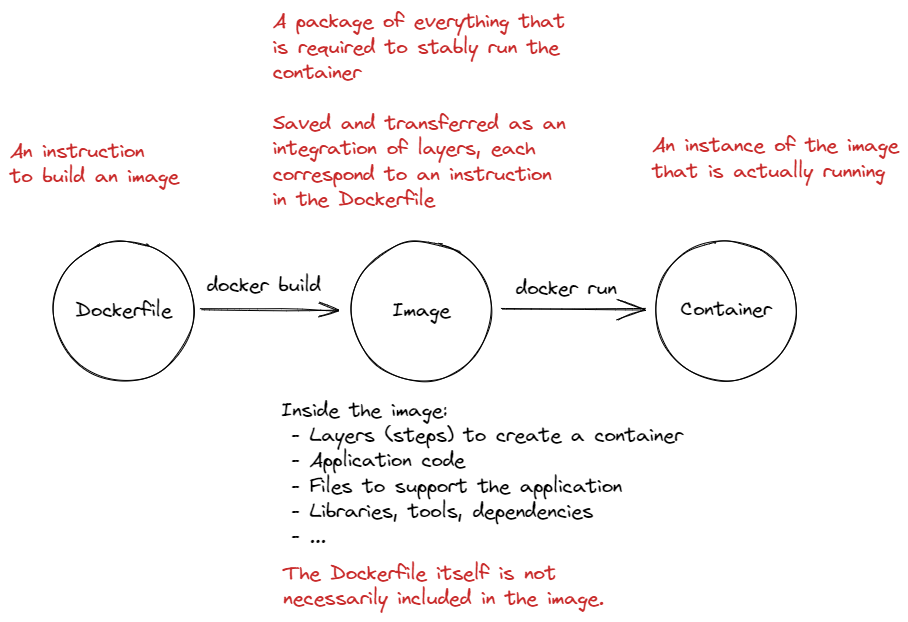
\includegraphics[width=350pt]{chapters/part-3/figures/dockerfiletoimage.png}
	\caption{A demonstration of how Dockerfile, image and container link to each other.} \label{ch:vac:fig:dockerfiletoimage}
\end{figure}

Since a docker image's primary role is to serve as a template for containers, many Dockerfile commands appear like a ``step-by-step'' recipe for container creation. Each instruction corresponds to an ``image layer''. An image is, in essence, an amalgamation of these layers. It is stored and distributed in this format. If images share layers (for instance, different versions of the same app), these shared layers are not saved or transferred redundantly, hence significantly reducing image sizes. More details can be found at \textit{https://docs.docker.com/storage/storagedriver/}.

\begin{shortbox}
\Boxhead{Docker Image Layers}

Docker containers employ a special file system known as the Union File System (UFS), which is well suited to the ``layer'' concept. UFS facilitates file sharing between the container and the host machine, along with combining read-only upper layers and writable lower layers, among other functions. 

A demonstration to illustrate this concept is given in Fig. \ref{ch:vac:fig:dockerlayerdemo}.

\end{shortbox}

\begin{figure}[!htb]
	\centering
	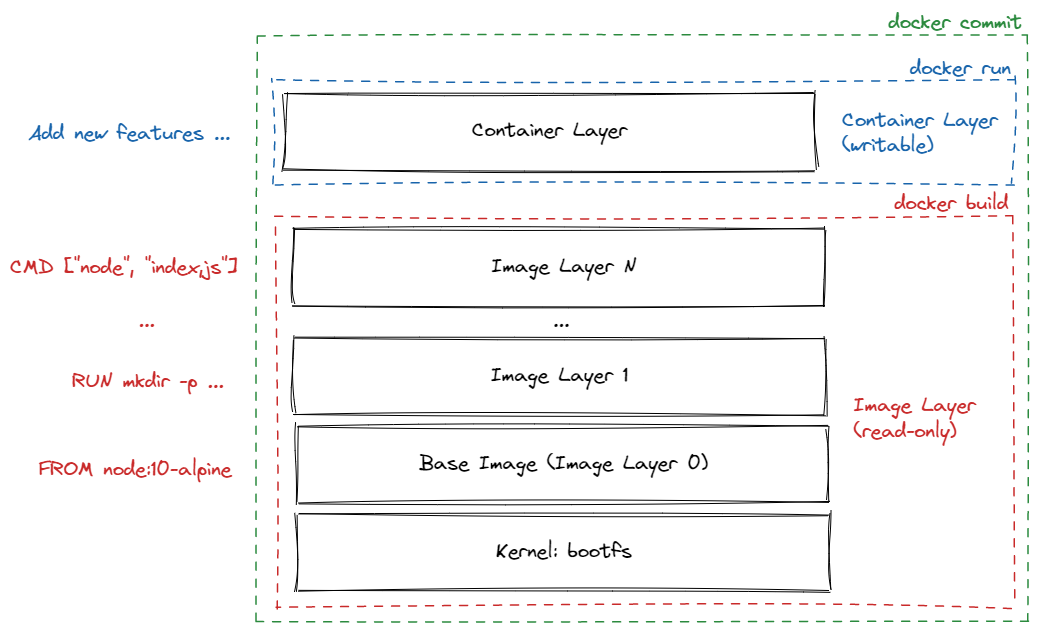
\includegraphics[width=350pt]{chapters/part-3/figures/dockerlayerdemo.png}
	\caption{A demonstration of docker image layer structure.} \label{ch:vac:fig:dockerlayerdemo}
\end{figure}

Just as a quick example, the Dockerfile to build the official \textit{hello-world} image from docker hub looks like the following.
\begin{lstlisting}
FROM scratch
COPY hello /
CMD ["/hello"]
\end{lstlisting}
In the example above, \verb|FROM scratch| signifies that this image is a base image without a parent. The \verb|COPY hello /| instruction copies the \textit{hello} binary script from the image to the root directory of the container. Lastly, \verb|CMD ["/hello"]| runs the \textit{hello} binary script.

In general, a typical Dockerfile includes the following instructions to build an image. These instructions allow the image to know how to create a container, automatically construct the file system directory structure, install necessary packages, and run the app:
\begin{enumerate}[(1)]
  \item Define parent image.
  \item Create filesystem directory.
  \item Set working directory.
  \item Copy files.
  \item Configure registry.
  \item Install packages.
  \item Copy more files after package installation.
  \item Switch to the correct user.
  \item Expose port.
  \item Run the application.
\end{enumerate}

The commonly used keywords to be used in a Dockerfile to realize the above instructions, such as \verb|FROM|, \verb|RUN|, are explained in Table \ref{ch:vac:tab:keywordsdockerfile}. 

It is worth highlighting the distinction between \verb|RUN| and \verb|CMD|. The \verb|RUN| command is executed during the building of the image, which creates a virtual representation of the environment to run the service. Therefore, \verb|RUN| is used to prepare the environment, for example, to install necessary libraries. On the other hand, command \verb|CMD| simply specifies the default command to run when the container starts. It is in built together with the image, but not considered as a read-only image layer. Indeed, the contents in \verb|CMD| can even be overwritten if the user wishes to do so when \verb|docker run| executes.

\begin{table}[!htbp]
	\centering \caption{Critical keywords used in a Dockerfile.}\label{ch:vac:tab:keywordsdockerfile}
	\begin{tabularx}{\textwidth}{lX}
		\hline
		Syntax & Description \\ \hline
		\verb|FROM <image>[:<tag>]| & Define the parent image. A Dockerfile must start with a \verb|FROM| instruction. A Dockerfile can contain multiple \verb|FROM| instructions for multi-stage build, in which case the last \verb|FROM| statement is the base image of the outcome image and the earlier \verb|FROM| instructions creates intermediate images that can be used by the outcome image. An optional \verb|:<tag>| following \verb|<image>| can be used to specify the version of the image to use as the base. By default, the latest version of the image is used. \\ 
		\verb|RUN <command>| & Execute a shell command using \verb|/bin/sh -c|. \\ 
		\verb|WORKDIR <path>| & Set the working directory from the point onward. This prepares the working directory for the upcoming \verb|RUN|, \verb|COPY|, etc., commands. \\ 
		\verb|ADD <src> <dest>| & Add (Copy) \verb|<src>|, either a directory/file or URL, to \verb|<dest>|. An optional \verb|[--chown=<user>:<group>]| can be used to specify the owner and group of the added files. \\ 
		\verb|COPY <src> <dest>| & Copy \verb|<src>|, a directory/file, to \verb|<dest>|. An optional \verb|[--chown=<user>:<group>]| can be used to specify the owner and group of the added files. Notice that \verb|COPY| is similar with \verb|ADD|. \verb|COPY| is easier but less powerful than \verb|ADD|. It cannot handle tar or URL. \\ 
		\verb|USER <user>| & Switch user for the instructions beyond this point. \\ 
		\verb|EXPOSE <port>| & Specifies the ports that the container shall listen to. An optional \verb|/<protocol>| following \verb|<port>| can be used to specify the protocol for communication. \\
        \verb|VOLUME ["<path>"]| & Attaches an anonymous volume to the specified path inside the container. \\
		\verb|CMD ["<exe>", "p1", ...]| & The user-script command. This is the last instruction in the Dockerfile that usually starts the APP. Notice that a Dockerfile can only contain one \verb|CMD| instruction. The executable command name and the parameters are put into a list. This user-script can be overwritten by \texttt{docker run <image> <other commands>} when running the container. \\
		\hline
	\end{tabularx}
\end{table}

Besides Table \ref{ch:vac:tab:keywordsdockerfile}, there are other Dockerfile keywords that can significantly simplify the design and maintenance of the image. For example, \verb|ENV <key>=<value>| assign a value to an environmental variable which can later be referred as \verb|$<key>| in the Dockerfile. An example is given below.
\begin{lstlisting}
ENV PORT=80
EXPOSE $PORT # this is interpreted as EXPOSE 80
\end{lstlisting}
Notice that environmental variables are accessible by the application code. They can be overwritten during \verb|docker run|. This means that the user can potentially use environmental variable to dynamically change the behavior of the application in the container when using \verb|docker run|. There are several benefits of doing this, for example, to enhance security. For example, if there is a password that the user needs to key in during the start of the container, the developer may want to put it as environmental variable and let the user to fill in, instead of hardcode the password in Dockerfile.

Another useful features of Dockerfile is the Dockerfile argument. It leaves a ``space'' in the Dockerfile that the developer can later fill in when he builds the image. An example is given below.
\begin{lstlisting}
ARG DEFAULT_PORT[=80]
ENV $DEFAULT_PORT
EXPOSE $PORT
\end{lstlisting}
The default value \verb|[=80]| is optional. When building the image, use \verb|--build-arg <variable-name>=<value>| to override the argument value. Notice that unlike environmental variables, Dockerfile arguments are not accessible by the application code or by the \verb|CMD| instruction.

Additionally, \verb|LABEL <key>="<value>"| assigns a tag to the image, which can be displayed when \verb|docker inspect <container>| is used.

Dockerfile programming can be very flexible and complicated at the same time. The advanced materials goes beyond the scope of this notebook.

Examples of Dockerfiles are given below, one from \textit{docs.docker.com} and the other from Linux Academy. The docker image layer structure of the second example is given in Fig. \ref{ch:vac:fig:dockerlayerdemo} as a demonstration. Notice that in Fig. \ref{ch:vac:fig:dockerlayerdemo}, \verb|bootfs| refers to the ``boot file system'', including the bootloader and the Linux kernel. Upon creation of a container using \verb|docker run|, a container layer will be added to the image, as shown by the blue dashed box in Fig. \ref{ch:vac:fig:dockerlayerdemo}. In the container, all the changes made is saved into the container layer.

To generate a new image to include the changes made in the container, use \verb|docker commit|, which essentially commits the container layer as the latest image layer in the new image, as shown by the green dashed box in Fig. \ref{ch:vac:fig:dockerlayerdemo}.

\begin{lstlisting}
# First Example
FROM golang:1.16
WORKDIR /go/src/github.com/alexellis/href-counter/
RUN go get -d -v golang.org/x/net/html
COPY app.go ./
RUN CGO_ENABLED=0 GOOS=linux go build -a -installsuffix cgo -o app .

FROM alpine:latest
RUN apk --no-cache add ca-certificates
WORKDIR /root/
COPY --from=0 /go/src/github.com/alexellis/href-counter/app ./
CMD ["./app"]
\end{lstlisting}

\begin{lstlisting}
# Second Example
FROM node:10-alpine
RUN mkdir -p /home/node/app/node_modules && chown -R node:node /home/node/app
WORKDIR /home/node/app
COPY package*.json ./
RUN npm config set registry http://registry.npmjs.org/
RUN npm install
COPY --chown=node:node . .
USER node
EXPOSE 8080
CMD ["node", "index.js"]
\end{lstlisting}

With the Dockerfile ready, use \verb|docker build| to build an image. An example is given as follows.
\begin{lstlisting}
$ docker build <path/url> -t <image name>
\end{lstlisting}
or
\begin{lstlisting}
$ docker build <path/url> -t <user name>/<image name>:<tag>
\end{lstlisting}
where \verb|<path/url>| is the path or URL to the directory where the Dockerfile locates (does not need to contain ``\verb|/Dockerfile|'' in its end), and \verb|-t| gives a tag, in this case an image name, to the image to build. For the convenience of sharing, it is recommended that all images to be pushed to a public registry (such as Docker Hub) shall be tagged with user name and version. Notice that the tag can be changed later after the image is built.

It is worth mentioning that \verb|docker build| builds the images by layers in the Dockerfile, and it will not re-build the same layer to which point no changes are made. This feature suggests that we should put the common and static layers in the early part of Dockerfile, and customized and user-defined layers in the late part, thus making the building (and also sharing, as will be introduced later) of the images more efficient.

Use \verb|.dockerignore| to exclude any files that should not be built into the image. Such files may include caches, the Dockerfile itself, etc.

\subsection{Docker Image Management}

The most commonly used image operations can be categorized as follows.
\begin{itemize}
  \item Create an image.
  \item Create a container from an image.
  \item Upload and download an image from a remote server.
  \item Manage local images, such as listing down all images, deleting an image, etc.
\end{itemize}

The first two operations have been introduced in earlier sections. The third and last ones are introduced below. Use the following command to search for an image on the default remote repository server (Docker Hub).
\begin{lstlisting}
$ docker search <image name>
\end{lstlisting}
Use the following command to download or update an image from the default remote repository server as follows. Notice that different from \verb|docker run|, this command will not start a container from the image.
\begin{lstlisting}
$ docker pull <image name>
\end{lstlisting}
Notice that since images are stored by layers, if two images share common layers, it is unnecessary to pull the shared layers repeatedly when downloading the second image, if the first image already exists in the host machine. Command \verb|docker pull| is smart enough to automatically detect shared layers, and avoid duplicating download of layers.

Use the following commands to list down or remove images.
\begin{lstlisting}
$ docker image ls
$ docker image rm <image name>
$ docker rmi <image name> # same as docker image rm
$ docker image prune # remove all problematic images
$ docker image prune -a # remove all unused images
\end{lstlisting}
where \verb|prune| removes all problematic images, and \verb|prune -a| removes all unused images from local.

Use the following command to inspect an image, and list down its metadata details.
\begin{lstlisting}
$ docker image inspect <image name>
\end{lstlisting}

\subsection{Docker Image Sharing with Docker Hub}

There are two ways to share an image:
\begin{itemize}
	\item Share the Dockerfile and APP source code so that the receiver can build docker image from his end.
	\item Share the image directly.
\end{itemize}
It is often more convenient to share the built image instead of the Dockerfile and the source code. However, a docker image is stored and managed by layers and cannot be shared simply by file transfer. 

Docker Hub is a commonly used server for storing and sharing docker images. It is also the default remote repository server of docker engine. However, do notice that Docker Hub is not the only remote docker image server. Some alternatives are Amazon Elastic Container Registry, Red hat Quay, Azure Container Registry, Google Container Registry, etc.

After registering an account on docker bub, use the following command to login to the Docker Hub from your local machine.
\begin{lstlisting}
$ docker login --username=<user name>
Passowrd:
\end{lstlisting}

Assume that there is an image in the local machine, and an empty repository on Docker Hub. In order to push the local image to the Docker Hub, the first step is to add the remote repository and the ``\textit{RepoTags}'' in the local image as follows.
\begin{lstlisting}
$ docker tag <image name> <user name>/<repository name>:<version>
\end{lstlisting}
where \verb|<version>| is a tag usually used to distinguish the different branches or versions of the images on Docker Hub. For the first image upload, it can simply be \verb|latest|.

Use the following command to push the image to Docker Hub.
\begin{lstlisting}
$ docker push <user name>/<repository name>
\end{lstlisting}

Notice that when using \verb|docker run| on an image with out a specified version and the image is not stored locally, Docker will automatically search and pull the latest version of that image from the remote repository, usually Docker Hub by default. However, if the image already exists locally, Docker simply uses that image and will not automatically check the remote repository for the latest version. To update the local image, manually use \verb|docker pull| to pull the latest or specific version of the image from the remote repository.

\section{Multi-Container Orchestration}

As introduced earlier, docker engine can be used to build and share images as well as start, monitor, and stop containers. It can be difficult for a user to manage containers manually when a lot of them are deployed. Container orchestrators such as Portainer and Kubernetes are helpful with managing containers. Many of these tools are able to automatically adjust the number of containers and balance their loads.

Many applications nowadays are multi-service multi-container applications. This trend has made container orchestration very useful in practice.

\subsection{Docker Compose}

Consider building and launching a multi-container applications. Multiple \verb|docker build| and \verb|docker run| commands need to be executed in specific order, and each command coming with a long list of arguments. Doing this manually can be tedious and introduce a high chance of human error.

A docker compose file is essentially a configuration file in YAML, usually named \verb|docker-compose.yml| (in later versions of docker compose, it can also be named \verb|compose.yml|). It plays as the user script or configuration file that automate the processes. Docker compose can process that configuration file, then build and launch containers accordingly. From that sense, docker compose can be seen as a container orchestration tool. 

This section gives a brief introduction to the preparation of a docker compose file. Examples of docker compose files can be found elsewhere online, such as \texttt{github.com/docker/awesome-compose}. 

A typical docker compose file looks like the following.

\begin{lstlisting}
version: "<compose file format version>"
services:
  <container name 1>:
    image: "<image name>"
    container_name: "<container name>"
    volumes:
      - <volume name 1>:<container path> # named volume
      - <container path> # anonymous volume
      - <host path>:<container path> # bind mount
      - ...
    environment:
      - <variable name 1>=<value 1>
      - <variable name 2>=<value 2>
      - ...
    env_files:
      - <path to environmental variable file 1>
      - <path to environmental variable file 2>
      - ...
    networks:
      - <network name>
    ports:
      - "<host port>:<contianer post>"
  <container name 2>:
    build:
      context: <path to Dockerfile directory>
      dockerfile: <name of docker file>
    volumes:
      - <volume name 2>:<container path> # named volume
      - <container path> # anonymous volume
      - <host path>:<container path> # bind mount
      - ...
    environment:
      - <variable name 1>=<value 1>
      - <variable name 2>=<value 2>
      - ...
    env_files:
      - <path to environmental variable file 1>
      - <path to environmental variable file 2>
      - ...
    networks:
      - <network name>
    ports:
      - "<host port>:<contianer post>"
    depends_on:
      - <container name>
      - ...
volumes:
  <volume name 1>: # for named volumes only
  <volume name 2>:
  ...
\end{lstlisting}
Some highlights are as follows.
\begin{itemize}
	\item \verb|version| tells the the compose file format version. Docker compose will then parse the compose file accordingly. 
	
	Different compose file format version may support different fields. If the version field is omitted, the composed file is parsed according to the latest version.
	
	\item \verb|services| describes the container(s) to be deployed. Each container is corresponding with a subcomponent under services.
	
	For simple containers whose image is readily available without \verb|docker build|, the following fields are commonly used in the subcomponent.
	
	\begin{itemize}
		\item \verb|image| specifies the image.
		\item \verb|container_name| specifies the container name; if not specified, default names will be used which are still human-readable.
		\item \verb|volumes| defines volumes and bind mounts.
		\item \verb|environment| defines environmental variables. 
		\item \verb|env_file| includes a file inside which are environmental variables.
		\item \verb|networks| adds the service to a docker network. Notice that this is often not necessary as all the services will be automatically added to the same newly created default docker network by default, unless a network is specified.
		\item \verb|ports| maps host ports to container ports.
		\item \verb|depends_on| lists containers that need to be launched before the current container.
	\end{itemize}
	
	In the case where a new image needs to be built before launching the container, docker compose file requires the following fields to build the image.
	
	\begin{itemize}
		\item \verb|build| gives the paths to the docker file.
		
		\begin{itemize}
			\item \verb|context| gives the directory of the docker file. Everything to be built into the image must be in this directory or its subdirectories.
			\item \verb|dockerfile|: the name of the Dockerfile.
		\end{itemize}
		
		Notice that one can simply use \texttt{build: <context>} if Dockerfile is named \verb|Dockerfile|.
		
	\end{itemize}
	
	\item \verb|volumes| lists all the named volumes used by the services.
\end{itemize}

A docker compose file example is given below. This example is taken from \texttt{awesome-compose} on GitHub. 
\begin{lstlisting}
version: "3.8"
services:
  web:
    image: nginx
    volumes:
      - ./nginx/nginx.conf:/tmp/nginx.conf
    environment: 
      - FLASK_SERVER_ADDR=backend:9091  
    command: /bin/bash -c "envsubst < /tmp/nginx.conf > /etc/nginx/conf.d/default.conf && nginx -g 'daemon off;'" 
    ports:
      - 80:80
    depends_on:
      - backend
  backend:
    build:
      context: flask
      target: builder
    # flask requires SIGINT to stop gracefully
    # (default stop signal from Compose is SIGTERM)
    stop_signal: SIGINT
    environment:
      - FLASK_SERVER_PORT=9091
    volumes:
      - ./flask:/src
    depends_on:
      -  mongo  
  mongo:
    image: mongo
\end{lstlisting}

Finally, execute docker compose as follows.
\begin{lstlisting}
$ docker-compose up -d
\end{lstlisting}
if the docker compose file is named as the default name (usually \verb|docker-compose.yml|), or
\begin{lstlisting}
$ docker-compose -f <docker compose file name> up -d
\end{lstlisting}
if otherwise. Docker images shall be built and containers be launched accordingly. And to shutdown all the services, simply use
\begin{lstlisting}
$ docker-compose down
\end{lstlisting}

Docker compose would not re-build the images by default if it thinks that the images it will use have been built before. To enforce rebuild, consider using \verb|--build| flag. Alternatively, use 
\begin{lstlisting}
$ docker-compose build
\end{lstlisting}
to build the images in the docker compose file without launching any container.

\subsection{Portainer}

Portainer is an open-source container management tool. It has a web-based dashboard user interface. Notice that Portainer itself also runs in a container.

Before starting a Portainer container, it is a good practice to first create a docker volume for Portainer to store the database. Use the following command to create such docker volume.
\begin{lstlisting}
$ docker volume create portainer_data
\end{lstlisting}
Then run a Portainer container using
\begin{lstlisting}
$ docker run -d -p 8000:8000 -p 9000:9000 -p 9443:9443 --name portainer --restart=always -v /var/run/docker.sock:/var/run/docker.sock -v portainer_data:/data portainer/portainer-ce
\end{lstlisting}
where ports 8000, 9000 and 9443 are used for hosting HTTP traffic in development environments, hosting web interface, and hosting HTTPS or SSL-secured services, respectively. The \verb|docker.sock| is the socket that enables the docker server-side daemon to communicate with its command-line interface. The image name for Portainer community edition (distinguished form the business edition) is \verb|portainer/portainer-ce|.

Use \verb|https://localhost:9443| to login to the container. The following page in Fig. \ref{ch:vac:fig:portainerlogin} should pop up in the first-time login, asking the user to create and administration user.
\begin{figure}[htbp]
	\centering
	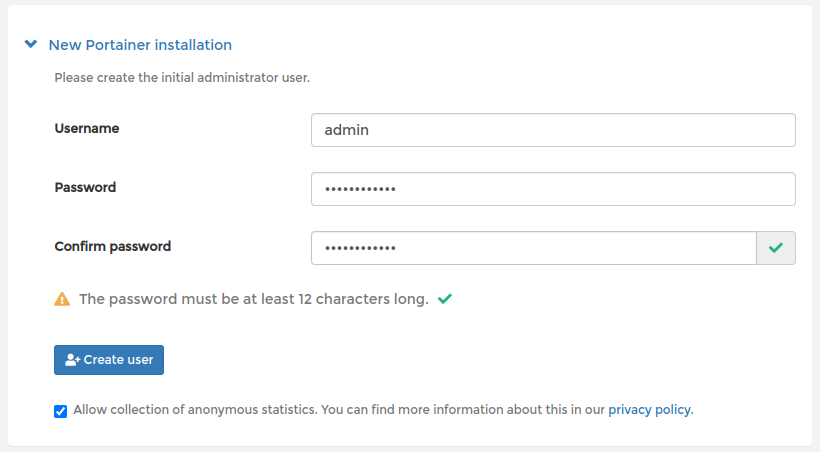
\includegraphics[width=350pt]{chapters/part-3/figures/portainerlogin.png}
	\caption{Portainer login page to create admin user.} \label{ch:vac:fig:portainerlogin}
\end{figure}

After creating the admin user and logging in, the status of images, containers and many more can be monitored via the dashboard, as shown in Figs. \ref{ch:vac:fig:portainerdashboard1}, \ref{ch:vac:fig:portainerdashboard2} and \ref{ch:vac:fig:portainerdashboard3}. Notice that in Fig. \ref{ch:vac:fig:portainerdashboard3}, using the ``quick action'' buttons, the user can check the specifics of the container and interact with its console, just like using \verb|docker container inspect| and \verb|docker exec|
\begin{figure}[htbp]
	\centering
	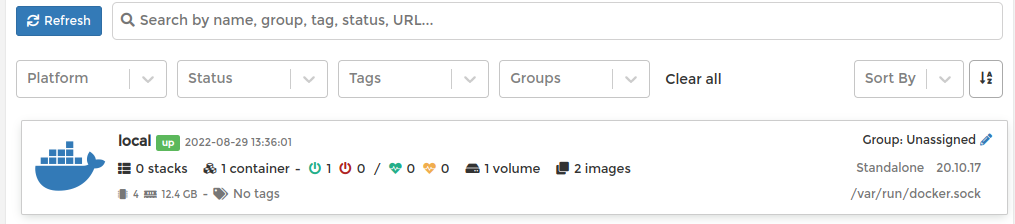
\includegraphics[width=350pt]{chapters/part-3/figures/portainerdashboard1.png}
	\caption{Portainer dashboard overview of docker servers.} \label{ch:vac:fig:portainerdashboard1}
\end{figure}

\begin{figure}[htbp]
	\centering
	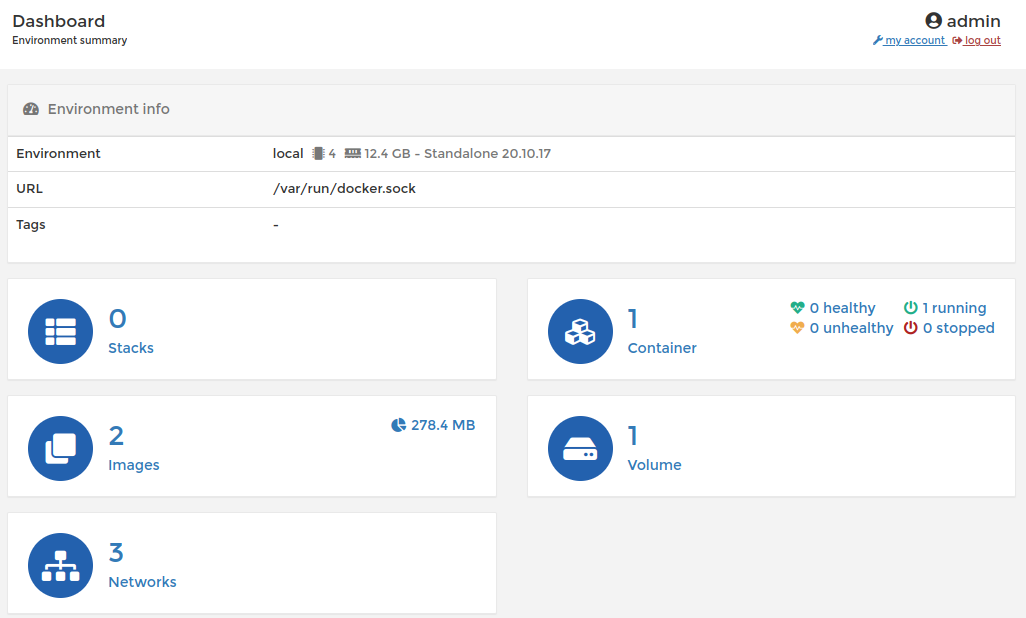
\includegraphics[width=350pt]{chapters/part-3/figures/portainerdashboard2.png}
	\caption{Portainer dashboard overview in a docker server.} \label{ch:vac:fig:portainerdashboard2}
\end{figure}

\begin{figure}[htbp]
	\centering
	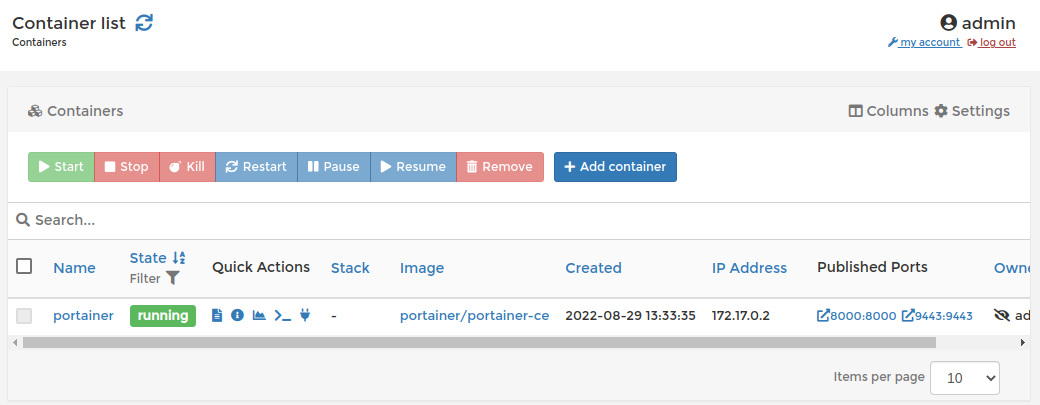
\includegraphics[width=350pt]{chapters/part-3/figures/portainerdashboard3.png}
	\caption{Portainer dashboard list down of all running containers.} \label{ch:vac:fig:portainerdashboard3}
\end{figure}

In summary, Portainer is an easy-to-use container management tool with clean graphical interface that a user can quickly get used to without a steep learning curve.

\section{Container Deployment in Production Environment}

So far we have been discussing container development and local testing. One of the most important selling points of containerization is that it is easy to ship applications. This is because the environment that supports an application is packaged together with the application in the image, which ensures that the application can run consistently whatever the host server is. 

Nevertheless, when the application is pushed to production environment, some adjustments need to be made. To name a few, below is a list of probable adjustments when shipping from development to production.

\begin{itemize}
	\item Bind mounts should not be used. Use \verb|COPY| to encapsulate all the resources needed, and use volume if data persistence is required.
	\item Some container setups may need to be changed.
	\item For multi-container applications, the containers may need to be deployed on multiple hosts.
\end{itemize}

This section discusses the deployment of containers on the cloud in production environment. Notice that for large scale applications deployment in the production environment, container orchestration tool such as Kubernetes is almost certainly necessary. Kubernetes and its cloud deployment are discussed in the later chapter and they are not considered in this section. 

\subsection{Docker-Supporting Hosting Providers}

Assume that the application can run correctly on the host machine. To deploy it on the Internet and allow public access, the first step is to find a docker-supporting hosting provider. There are many such providers, the most popular of which include Amazon Web Services (AWS), Microsoft Azure and Google Cloud. They are not just docker hosting providers but more general cloud services providers.

Details about the cloud services providers and cloud computing are beyond the scope of this notebook. Only the services relevant to container deployment are introduced here. AWS is considered.

\subsection{EC2-Based Approach}

The most intuitive way to deploy containers on AWS is to use EC2. To do that, the following steps are required.

\begin{enumerate}
	\item Start EC2, and enable SSH access to the EC2 from the local machine.
	\item Install docker on the EC2 instance.
	\item Upload the images which have been built in the local machine to the EC2 instance.
	\item Start the containers on EC2.
	\item Enable public access to the EC2 by publishing its IP address.
\end{enumerate}

Notice that EC2-based deployment is not the best practice as AWS and many other cloud service providers have managed container management services such as Elastic Container Service (ECS) and Elastic Kubernetes Service (EKS). However, for illustration purpose, we will start from EC2-based deployment.

The key steps to launch and connect to a EC2 instance from a Linux local machine are given below.
\begin{enumerate}
  \item Create and configure the EC2 instance from AWS dashboard.
  \item In the last step of EC2 instance configuration, create or select a key pair. The key pair is used later to SSH to the instance. Download the private key pair. The name of the private key pair is by default \verb|<key pair name>.pem|. 
  \item Change the ACL of the private key pair to \verb|400| to disable public view using \texttt{chmod 400 <key pair name>.pem}.
  \item Launch the EC2 instance from AWS dashboard. Wait until the instance state becomes ``running''. Locate the public DNS of the instance from the dashboard which usually looks like \texttt{<serial number>.<region>.compute.amazonaws.com}.
  \item SSH to the EC2 instance using \texttt{ssh -i "<key pair name>.pem" <username>@<public dns>}.
\end{enumerate}
To install and start docker on the EC2 instance, use
\begin{lstlisting}
$ sudo yum update -y
$ sudo yum install docker
$ sudo systemctl start docker
\end{lstlisting}
To upload an image from the local machine to the EC2 instance, use Docker Hub as a bridge. The user can then launch containers on the EC2 instance the same way he would do on a local machine. Lastly, to enable public access to the EC2 from HTTP, configure the security group inbound rules attached to the EC2 instance. By default, the only allowed inbound rule is SSH using TCP protocal via port range 22 from all IP addresses. Depending on the applications running on the EC2 instance, the user may want to add more inbound rules, for example, enabling HTTP/HTTPS access via port 80.

For multi-container applications, the user can upload all necessary images to Docker Hub, and on the EC2 instance simply execute a docker compose file. Notice that the docker compose file should use the images on Docker Hub instead of building any on the fly. In production environment, all the images should be pre-built.

The EC2-based approach has some disadvantages compared with ECS and EKS that will be introduced in later sections. There are at least the following disadvantages.
\begin{itemize}
  \item Lack of robustness. EC2 belongs to the Infrastructure as a Service (IaaS) family where AWS only supports the infrastructure (in this case, the VM) and not anything running on it (in this case, docker and the containerized application). The user needs to deal with all the ``accidents'' that may break the system such as someone launching a cybor attack on the VM. This makes the solution less robust.
  \item Difficult to scale. The total computational power of the application depends on the setup of VM which is pre-determined and cannot be easily scaled up or down on the fly.
  \item Difficult to manage. The user needs to SSH to the VM to audit and upgrade the applications, which can become annoying.
\end{itemize}
This makes EC2-based container approach almost always suboptimal compared with ECS and EKS.

\subsection{Managed-Service-Based Approach}

ECS and EKS are the recommended manages service of AWS for containerized applications. EKS will be introduced in the later chapter with Kubernetes. This section discusses ECS. 














\chapter{Kubernetes}

Kubernetes is one of the most widely used container orchestration tools. Many cloud platforms provide Kubernetes support. Many opponent container orchestration tools are built on top of Kubernetes.

\section{Kubernetes Basics}

\mync{Kubernetes}, also known as \mync{k8s}, is an open-source container orchestration system originally developed by Google. It automates the deployment, health screening and scaling of containers for containerized applications.

As an orchestration tool, Kubernetes mainly focuses on the following tasks:
\begin{itemize}
	\item Monitor the status of the containers, and restart / replace broken ones.
	\item Balance the load assigned to the containers.
	\item Strategically scale up and down the number of containers based on the total load.
\end{itemize}
From the above, Kubernetes can be seen as a more powerful practice of what docker compose tries to do. It comes with additional features such as the support on multi-server deployment.

Managed services such as ECS can also do container orchestration. However, these managed services are often proprietary and inclusive to a particular cloud service provider. With such proprietary services, it is difficult to migrate the applications across platforms or to local premises. Kubernetes, on the other hand, is open-source and platform-independent, hence would not pose that problem.

Nowadays, many cloud service providers also support Kubernetes-based container deployment solutions such as \myabb{Elastic Kubernetes Service}{EKS} by AWS and \myabb{Google Kubernetes Engine}{GKE} by Google Cloud. They are also managed services to some extend and each platform usually have some unique features, but in general the application can be migrated across platforms without too much difficulty.

\begin{shortbox}
	\Boxhead{Kubernetes and Docker Engine}
	
	Kubernetes was built on top of docker engine. It used a special program \verb|dockershim| to talk to the underlying docker engine. Recently, however, docker support has been deprecated in Kubernetes. Consequently, \verb|dockershim| has also been removed. Now Kubernetes directly talks with container runtimes.
\end{shortbox}


\subsection{Infrastructure}

Figure \ref{ch:vac:fig:kubernetescluster} demonstrates the key components Kubernetes has inside its cluster.
\begin{figure}[!htb]
	\centering
	\includegraphics[width=250pt]{chapters/part-3/figures/k8sarchitecture.png}
	\caption{Kubernetes cluster and its key components.} \label{ch:vac:fig:kubernetescluster}
\end{figure}
As shown in Fig. \ref{ch:vac:fig:kubernetescluster}, Kubernetes manages containers in a centralized ``master-worker'' manner, where the \mync{master node} (also known as \mync{control plane}) in yellow interacts with the user and schedules the Pods to be deployed for each work node. The \mync{work nodes} (also known as \textbf{nodes}, for short) in green, on the other hand, process the application data. The arrows in Fig. \ref{ch:vac:fig:kubernetescluster} represents the control flow. Notice that the application data flows differently and it does not pass through the master. There can be multiple master nodes (in replica mode) and worker nodes, though only one of each is shown in Fig. \ref{ch:vac:fig:kubernetescluster}.

Key components in the master and the nodes and their functions are summarized in Table \ref{ch:vac:tab:keycomponents}.

\begin{table}[!htb]
	\centering
	\caption{Key components in Kubernetes master and nodes.} \label{ch:vac:tab:keycomponents}
	\begin{tabularx}{\textwidth}{llX}
		\hline
		Component & Location & Description \\
		\hline
		\verb|etcd| & Master & A distributed key-value pair database that stores the status of the Kubernetes cluster. The consistency of the distributed database is achieved based on Raft consensus algorithm. \\ \hline
		API server & Master & The gateway to handle all interactions with the Kubernetes cluster. For example, \verb|kubectl| requests from the user are handled by API server. \\ \hline
		Scheduler & Master & The optimizer that calculates the desired Pod distributions among all nodes based on the total load and the hardware limits. Notice that scheduler is not involved into load balance directly. A separate load balancer service can be created to actually direct the traffic. \\ \hline
		Controller Manager & Master & A set of controllers or control functions to reconcile the actual Kubernetes cluster status with what has been calculated by the scheduler and stored in \verb|etcd|. \\ \hline
		Kubelet & Node & Local controller for the node. It ensures that all the Pods assigned to the node are running, and it keeps listening to the master for further instructions. \\ \hline
		Kube Proxy & Node & The internet service provider in the node. \\
		\hline
	\end{tabularx}
\end{table}

Each node can host multiple Pods. A Pod object is a single container or a collection of containers for a single task, and it is also the smallest unit that Kubernetes controls directly. Notice that in Kubernetes, containers never run directly in a node. They are always grouped into Pods. More details about the Pod object are introduced in later Section \ref{ch:vac:sec:objects}.

Both master and nodes can run on multiple servers or VMs. For master, multiple master replicas can run in parallel to take care of user requests and provide database services. The ``decision makers'', i.e. the controller manager and scheduler, run only on one of the master nodes which is elected via a leader election process. Should the decision maker master fail, one of the replicas will be promoted. For nodes, multiple nodes can run together to precess information in parallel and Kubernetes manages the distribution of load among them.

It is worth mentioning that many services cluster-level services such as ClusterIP, NodePort, LoadBalancer and Ingress Controllers, though being cluster-level, run in worker nodes but not in the master. 

\subsection{Installation}

Kubernetes is not a single piece of software but more an architecture that involves many pieces of software such as:
\begin{itemize}
  \item \verb|kubectl| the CLI
  \item \verb|kube-apiserver| the API server
  \item \verb|etcd| the distributed key-value pair database
  \item \verb|kube-scheduler| the scheduler
  \item \verb|kube-controller-manager| the control manager
  \item Kubelet
  \item Kube Proxy
  \item Kubernetes-supported container runtime such as \verb|containerd|
  \item Container Network Interface (CNI) plugin such as Calico
  \item \ldots
\end{itemize}
The installation guidance of Kubernetes can be found at its official website \textit{kubernetes.io}. In a production environment, the administrator shall install and configure the above tools on the servers by himself. This gives him the flexibility of customizing the tools. However, the process can be tedious and requires experience.

In this notebook, for demonstration purpose, we will use Minikube to help build a Kubernetes cluster. Minikube is an open-source software developed by the Kubernetes community to start a VM and run a single-node Kubernetes cluster on a local machine. It automates most of the tools installations and configurations which is in favour of the scope of this notebook. 

We still need to install Minikube and also \verb|kubectl|. As introduced earlier, \verb|kubectl| is used to interact with Kubernetes clusters deployed either locally or remotely. It is always recommended to have \verb|kubectl| installed on the local machine wherever the Kubernetes cluster is deployed. The installation of \verb|kubectl| can be found at Kubernetes website at
\begin{lstlisting}
https://kubernetes.io/docs/tasks/tools/install-kubectl-linux/
\end{lstlisting}
Minikube installation can be found at
\begin{lstlisting}
https://minikube.sigs.k8s.io/docs/start/
\end{lstlisting}

Once Minikube is installed, start it using
\begin{lstlisting}
$ minikube start
\end{lstlisting}
When starting Minikube, it automatically detects which container engine to use, and some configurations might be required subsequently.

When running Minikube, it uses existing VM engines such as VirtualBox, or container engines such as docker and podman installed on the local machine to start a VM or container that hosts Kubernetes. Therefore, it will need to execute the VM tools or the container engines. In naive RHEL, Minikube needs to execute podman. Some of the commands Minikube need to run require sudo privilege, and as a result, it requires \verb|NOPASSWD| configuration to start the Kubernetes cluster correctly. 

This can be done as follows. Open the sudoer configuration file by
\begin{lstlisting}
$ sudo visudo
\end{lstlisting}
and append
\begin{lstlisting}
<user name> ALL=(ALL) NOPASSWD: /usr/bin/podman
\end{lstlisting}
to the file.

Once Minikube is started, \verb|kubectl| installed on the local machine should be able to detect the Kubernetes running inside. Sse the following command to verify that \verb|kubectl| has detected and connected with the Kubernetes runtime.
\begin{lstlisting}
$ kubectl cluster-info
Kubernetes control plane is running at https://192.168.49.2:8443
CoreDNS is running at https://192.168.49.2:8443/api/v1/namespaces/kube-system/services/kube-dns:dns/proxy
\end{lstlisting}

\begin{shortbox}
\Boxhead{Minikube's Built-in \texttt{kubectl}}

Minikube also comes with a built-in \verb|kubectl|. It is possible to use that \verb|kubectl| instead of installing one separately. To very the existence of the built-in \verb|kubectl|, start Minikube first and then use

\begin{lstlisting}
$ minikube kubectl -- cluster-info
Kubernetes control plane is running at https://192.168.49.2:8443
CoreDNS is running at https://192.168.49.2:8443/api/v1/namespaces/kube-system/services/kube-dns:dns/proxy
\end{lstlisting}
where \verb|--| in the command tells the shell that all the followed arguments shall be passed to \verb|kubectl| inside Minikube, but not \verb|minikube| itself. For convenience, one may want to use alias as follows
\begin{lstlisting}
$ alias kubectl="minikube kubectl --"
\end{lstlisting}

With the above been said, it is still recommended that \verb|kubectl| to be installed on the local machine, not just in the VM. 
\end{shortbox}

It is possible to run Kubernetes cluster directly on a host machine OS without VM if that machine is running Linux. However, this is not recommended for reasons pertaining to access control, security, and isolation. It is generally a better practice to deploy Kubernetes clusters in VMs.

The configuration file for \verb|kubectl| is usually located at \verb|~/.kube/config|. It determines the basic setups of the \verb|kubectl| instance, such as which Kubernetes cluster \verb|kubectl| communicates with.

\subsection{Kubernetes Cluster Manipulation}

There are at least two ways for a user to interact with a Kubernetes cluster and deploy or manipulate services in it.
\begin{itemize}
  \item Imperative approach: use \verb|kubectl| commands to directly start, change or stop Pods and services.
  \item Declarative approach: prepare Kubernetes configuration files that describes the ``desired state'' of the Kubernetes cluster, and use \verb|kubectl -f| command to implement the files. Kubernetes decides how to deploy Pods on servers to achieve the desired state.
\end{itemize}
Both approaches are introduced as follows. 

\vspace{0.1in}
\noindent \textbf{Cluster Deployment with Imperative Approach}
\vspace{0.1in}

The imperative approach, in some sense, destroys the purpose of Kubernetes as a container orchestration tool since the user decides the deployment of Pods and services manually. On the other hand, the declarative approach takes advantage of the full capability of Kubernetes and it is usually considered a better practice. Yet, learning the imperative approach helps the user with getting familiar with \verb|kubectl| commands. In this section, imperative approach and its relevant generally used \verb|kubectl| commands are briefly introduced.

Use the following to view the entire list of \verb|kubectl| supported commands.
\begin{lstlisting}
$ kubectl help
kubectl controls the Kubernetes cluster manager.

 Find more information at: https://kubernetes.io/docs/reference/kubectl/

Basic Commands (Beginner):
  create          Create a resource from a file or from stdin
  expose          Take a replication controller, service, deployment or pod and expose it as a new Kubernetes service
  run             Run a particular image on the cluster
  set             Set specific features on objects

Basic Commands (Intermediate):
  explain         Get documentation for a resource
  get             Display one or many resources
  edit            Edit a resource on the server
  delete          Delete resources by file names, stdin, resources and names, or by resources and label selector

Deploy Commands:
  rollout         Manage the rollout of a resource
  scale           Set a new size for a deployment, replica set, or replication controller
  autoscale       Auto-scale a deployment, replica set, stateful set, or replication controller

Cluster Management Commands:
  certificate     Modify certificate resources
  cluster-info    Display cluster information
  top             Display resource (CPU/memory) usage
  cordon          Mark node as unschedulable
  uncordon        Mark node as schedulable
  drain           Drain node in preparation for maintenance
  taint           Update the taints on one or more nodes

Troubleshooting and Debugging Commands:
  describe        Show details of a specific resource or group of resources
  logs            Print the logs for a container in a pod
  attach          Attach to a running container
  exec            Execute a command in a container
  port-forward    Forward one or more local ports to a pod
  proxy           Run a proxy to the Kubernetes API server
  cp              Copy files and directories to and from containers
  auth            Inspect authorization
  debug           Create debugging sessions for troubleshooting workloads and nodes
  events          List events

Advanced Commands:
  diff            Diff the live version against a would-be applied version
  apply           Apply a configuration to a resource by file name or stdin
  patch           Update fields of a resource
  replace         Replace a resource by file name or stdin
  wait            Experimental: Wait for a specific condition on one or many resources
  kustomize       Build a kustomization target from a directory or URL

Settings Commands:
  label           Update the labels on a resource
  annotate        Update the annotations on a resource
  completion      Output shell completion code for the specified shell (bash, zsh, fish, or powershell)

Subcommands provided by plugins:

Other Commands:
  api-resources   Print the supported API resources on the server
  api-versions    Print the supported API versions on the server, in the form of "group/version"
  config          Modify kubeconfig files
  plugin          Provides utilities for interacting with plugins
  version         Print the client and server version information

Usage:
  kubectl [flags] [options]
\end{lstlisting}

Use
\begin{lstlisting}
$ kubectl create <object type> <object name> --<argument>
\end{lstlisting}
to create and deploy an object, and use
\begin{lstlisting}
$ kubectl get <object type>
\end{lstlisting}
to view deployed objects of certain type. Notice that in \verb|kubectl get| is usually followed by the plural form of the object type. An example is given below.
\begin{lstlisting}
$ kubectl create deployment <deployment name> --image=<image name>
$ kubectl get deployments
\end{lstlisting}
Deployment object is deployed in the above example. More about Deployment object will be given in later Section \ref{ch:vac:sec:objects}. It is one of the most commonly used Kubernetes objects and serves well as an example to illustrate imperative approach. Notice that the image assigned to the deployment, in the above example \texttt{hello-world}, needs to be reachable by Kubernetes. In this example, the image is to be deployed by the Kubernetes cluster deployed in the Minikube environment, and hence any image locally built in the host machine will not be reachable. The image has to be stored on an online registry.

The deployed Pods will be default have a cluster-level internal IP. There are the following problems with this internal IP: it is dynamic, and it is not accessible from outside the cluster. To expose the IP and port, a separate Service object needs to be used as follows.
\begin{lstlisting}
$ kubectl expose deployment <deployment name> --type=<service type>
\end{lstlisting}
where Service object type can be \verb|ClusterIP|, \verb|NodePort|, \verb|LoadBalancer|, etc. More about Service object will be given in later Section \ref{ch:vac:sec:objects}.

To scale up and down the number of Pods in a Deployment object, use
\begin{lstlisting}
$ kubectl scale --replicas=<number> deployment <deployment name>
\end{lstlisting}

And finally to update the image of the deployment, use
\begin{lstlisting}
$ kubectl set image deployment/<deployment name> <container name>=<image name: tag>
\end{lstlisting}
For example,
\begin{lstlisting}
$ kubectl set image deployment/nginx-deployment my-nginx-container=nginx:1.25.1
\end{lstlisting}

The user can check the status of the roll out by
\begin{lstlisting}
$ kubectl rollout status deployment/<deployment name>
\end{lstlisting}
When Kubernetes is rolling out a new version, the old version will not be shutdown. This minimizes the blackout time when an application is being updated.

The user can check the history of the roll out using
\begin{lstlisting}
$ kubectl rollout history deployment/<deployment name> [--revision=<revision index>]
\end{lstlisting}
where \verb|[--rivision]| will provides details to the roll out.

To roll back to an earlier version in the history, use
\begin{lstlisting}
$ kubectl rollout undo deployment/<deployment name> [--to-revision=<revision index>]
\end{lstlisting}
where if \verb|--to-revision| is not used, the command rolls back to the earlier latest version.

\vspace{0.1in}
\noindent \textbf{Cluster Deployment with Declarative Approach}
\vspace{0.1in}

Kubernetes configuration files describe the desired final status of the Kubernetes cluster. Should these files be passed to Kubernetes, it should be able to determine the processes to deploy relevant Kubernetes objects and eventually realize and maintain the desired state. This is known as the declarative approach and it is the default and recommended way Kubernetes shall be used. The declarative approach has at least the following advantages over the imperative approach:
\begin{itemize}
  \item It automates the Kubernetes deploying by using configuration files instead of the user running \verb|kubectl| commands manually, which simplifies the process and reduces human error.
  \item It leverages on the container orchestration capability of Kubernetes.
\end{itemize}
These advantages are critical especially in large-scale projects when there are multiple Kubernetes objects in the cluster.

The details of Kubernetes objects are introduced in later Section \ref{ch:vac:sec:objects}. In this section, a simple example is used to illustrate the basic commands for the declarative approach. Below is an example from the Kubernetes website. It contains the configuration of two objects.
\begin{lstlisting}
apiVersion: apps/v1
kind: Deployment
metadata:
  name: nginx-deployment
  labels:
    app: nginx
spec:
  replicas: 3
  selector:
    matchLabels:
      app: nginx
  template:
    metadata:
      labels:
        app: nginx
    spec:
      containers:
      - name: nginx
        image: nginx:1.14.2
        ports:
        - containerPort: 80
\end{lstlisting}

Some commonly used fields used in the Kubernetes configuration files are briefly summarized below.
\begin{itemize}
	\item \verb|apiVersion|: The API version of the object. Different object types are supported in different API versions.
	\item \verb|kind|: The object type.
	\item \verb|metadata|: The name and labels of the object. 
	\item \verb|spec|: The specifications of the object. Different object types require different specifications.
\end{itemize}
More details of the configuration file composing of each type of Kubernetes object are introduced in later Section \ref{ch:vac:sec:objects}. 

With the image and the configuration files ready, the next step is to deploy the nodes, Pods, and containers. The \verb|kubectl| CLI is used to instruct Kubernetes to deploy the objects as follows.
\begin{lstlisting}
$ kubectl apply -f <configuration file> / <files directory>
\end{lstlisting}
This essentially asks the master node in the Kubernetes cluster to start taking actions following the Kubernetes configuration files, such as to inform the nodes to start creating Pods and containers. The master node also keeps monitoring the status of each work node, to make sure that everything is running as planned. If there is a container failure, etc., the master node will guide the associated note to restart the container.

It is possible to consolidate the configuration files of objects into one configuration file. To do that, use \verb|---| to split the configurations for each object in the conjunctive configuration file as follows. It is of personal preference whether to use conjunctive configuration files or separate configuration files for all objects.
\begin{lstlisting}
<configurations for object 1>
---
<configurations for object 2>
---
<...>
\end{lstlisting}
The order of the configurations appears in the file usually does not matter. However, it is often considered a better practice to put cluster-level objects such as Service objects in front of work split objects such as Development objects.

With the help of Kubernetes declarative approach, it is possible to update the cluster simply by revising the configuration files, and pass them to Kubernetes as if the cluster is to be deployed for the first time. Kubernetes automatically checks revised configuration files, comparing them with existing running objects, and update them if necessary.

It is recommended to check the status of the Pods using \verb|kubectl get pods| once the cluster is updated. After the update, the Pods should be restarted, and hence the ``RESTARTS'' tag shall increase. To ensure that the update is successful, use \verb|kubectl describe| to check the details of the relevant objects.

Notice that there is a limitation on what can be updated to an existing Kubernetes deployment. For an existing object, only certain fields in the Kubernetes configuration files are allowed to be revised. For example, for a Pod, the image can be changed while the ports cannot. Some objects types are more flexible than others when comes to object updating. The user shall choose wisely what object types to use considering what updates need to be made in future.

To revert what has been applied in a Kubernetes configuration file, use
\begin{lstlisting}
$ kubectl delete -f <configuration file>
\end{lstlisting}
The user can also delete certain types of objects by labels by
\begin{lstlisting}
$ kubectl delete <object type 1>[, <object type 2>, ...] -l <label>
\end{lstlisting}

\vspace{0.1in}
\noindent \textbf{Kubernetes Cluster Status Check}
\vspace{0.1in}

To retrieve the status of a group of objects, use
\begin{lstlisting}
$ kubectl get <object type>
\end{lstlisting}
where \verb|<object type>| can be \verb|pods|, \verb|services|, etc. For more details of a specific object, use
\begin{lstlisting}
$ kubectl describe <object type> <object name>
\end{lstlisting}
for example, to check the containers running in a Pod. If \verb|<object name>| is neglected, Kubernetes returns detailed information of all objects of the given object type. For a running object, use
\begin{lstlisting}
$ kubectl logs <object name>
\end{lstlisting}
to check the log file of that object.

Minikube provides a web-based dashboard where the user can conveniently check the status of the cluster. Use
\begin{lstlisting}
$ minikube dashboard
\end{lstlisting} 
to start the dashboard and follow the instructions on the concole to open the dashboard. The dashboard gives the detailed information of running objects in the Kubernetes cluster, such as the healthy status of Pods, the cluster-level internal IP of objects, etc.


Kubernetes treats the above as an update and will action accordingly.

\section{Basic Kubernetes Objects} \label{ch:vac:sec:objects}

Kubernetes supports a long list of objects, and the list is growing along with Kubernetes version. The list can be displayed by
\begin{lstlisting}
$ kubectl api-resources
\end{lstlisting}

It is hardly possible to cover all the Kubernetes objects in this notebook. This section only introduces the commonly used basic Kubernetes objects summarized in Table \ref{ch:vac:tab:objtype}.
\begin{table}[!htb]
	\centering
	\caption{Commonly used Kubernetes object types.} \label{ch:vac:tab:objtype}
	\begin{tabularx}{\textwidth}{lX}
		\hline
		Object Type & Description \\
		\hline
		Pod & Represents a single instance of a process running in the cluster. A Pod contains one or multiple containers that work closely to deliver a basic function. It is the smallest unit of process in Kubernetes. \\ \hline
		Deployment & Manages the deployment and scaling of a set of identical Pods, ensuring the desired number of replicas are running and providing rolling updates for seamless application upgrades. \\ \hline
		Service & Enables network access to the node or to a set of Pods using a stable IP address and DNS name. It provides load balancing across multiple Pod replicas and allows external traffic to be directed to the appropriate Pods. \\ \hline
		ConfigMap & Stores configuration data in key-value pairs, which can be consumed by Pods as environment variables, command-line arguments, or mounted as files. \\ \hline
		Volume & Provides a way to provision and manage persistent storage resources in a cluster. \\
		\hline
	\end{tabularx}
\end{table}

\subsection{Pod Object}

\mync{Pod} object is the smallest and most fundamental unit in a node that Kubernetes interacts with. A Pod is essentially a ``wrap'' that hosts one or multiple containers that work closely with each other. Pod contains shared resources such as volumes for all the containers it hosts. The containers in a Pod can also communicate each other via \verb|localhost|. A Pod has a cluster-internal IP by default.

Just like a container, Pods are designed to be ephemeral. Kubernetes can start and stop them depending on the load and the traffic coming into the cluster, and when they are removed, their data vanishes. Of course there are many ways to persist the data, for example by directing the data into a volume or a database.

The user can deploy Pods using either \verb|kubectl| command imperatively or in Kubernetes configuration files declaratively. However, the user would not do so in practice, as it destroys the purpose of using Kubernetes.

A Pod is assigned with a cluster-level internal IP by default, and that IP can be used for communications inside the Kubernetes cluster. It has the following problems though, making the IP address difficult to use:
\begin{itemize}
  \item The IP address is internal the cluster, hence useless to entities outside the container.
  \item Even for communications inside the cluster, the IP address is not convenient to use since it is dynamic.
\end{itemize}

\subsection{Deployment Object}

It is more often that the user would want to deploy Deployment objects instead of Pods. A \mync{Deployment} object serves as the ``controller'' of one or a group of identical Pods, and it serves as a good example to illustrate declarative approach where the user specifies a desired state and the Deployment object carries out the necessary procedures to realize that state. A Deployment object can do at least the following for the Pods it manages:
\begin{itemize}
  \item Start and stop the Pods strategically at different word nodes.
  \item Monitor the healthy status of the Pods and strategically restart them when necessary.
  \item Scale up and down the number of Pods.
  \item Balance the loads that go into each Pod.
  \item Update or roll back the Pods.
\end{itemize}

As an example, a Kubernetes cluster file that deploys an Deployment object is given below. Notice that Deployment object is supported in API version \verb|apps/v1|.
\begin{lstlisting}
apiVersion: apps/v1
kind: Deployment
metadata:
  name: nginx-deployment
  labels:
    app: nginx
spec:
  replicas: 3
  selector:
    matchLabels:
      app: nginx
  template:
    metadata:
      labels:
        app: nginx
    spec:
      containers:
        - name: nginx
          image: nginx
          ports:
            - containerPort: 80
\end{lstlisting}
Some highlights under \verb|spec| are introduced below.
\begin{itemize}
	\item \verb|replicas|: the number of Pods under the Deployment object should maintain. The value can be zero if no Pods need to be deployed initially.
	\item \verb|selector.matchLabels|: a set of labels, which if a Pod possesses, will be monitored and likely managed by the Deployment object.
	\item \verb|template|: the template that describes the Pods this Deployment object creates, including:
    \begin{itemize}
      \item \verb|metadata.labels|: the labels the Pods will inherit.
      \item \verb|spec.containers|: the containers details, such as name, image, port, etc.
    \end{itemize}
\end{itemize}
Notice that a Deployment object can deploy only identical Pods from the same template. If different types of Pods need to be deployed, different Deployment objects are required. However, under one Pod, there can be multiple containers populated from different images. Notice that \texttt{template.spec.containers} contains a list of containers, each with its name, image, ports, etc. Append that list if multiple containers are required under the same Pod.

An alternative to \texttt{selector.matchLabels} is \texttt{selector.matchExpressions}, the later of which provides a more powerful and flexible way of mapping labels. More details of \texttt{selector.matchExpressions} is not introduced in this notebook, as \texttt{selector.matchLabels} should serve well in most scenarios.

\begin{shortbox}
\Boxhead{Labels in \texttt{selector} and \texttt{template}}

It may feel redundant that the same labels appear twice under both \texttt{selector.matchLabels} and \texttt{template.metadata.labels}. This sense of redundancy often stems from the assumption that a Deployment object should watch (and only watch) the Pods it creates.

In reality, multiple controllers can ``monitor'' the same Pods, potentially for metrics, auditing, or other read-only operations. A Pod has exactly one owner which is the controller that creates the Pod, but it can be monitored by other controllers or tools via label selector.

By splitting \texttt{selector.matchLabels} and \texttt{template.metadata.labels} instead of automatically inheriting one from the other, Kubernetes provides flexibility in how Pods and Deployment objects are architected. Additional labels can be added in the template to support other purposes—like monitoring, cost allocation or environment tagging without affecting the Deployment’s fundamental ownership of those Pods.

\end{shortbox}

When a new version of an image becomes available, we may want to update the containers accordingly. Re-apply the same configuration file would not help, as Kubernetes would reject apply request if no change is detected in the configuration file. It would not check whether the image is in its latest version. The following imperative command which has been introduced earlier can be used to update the image.
\begin{lstlisting}
$ kubectl set image deployment/<deployment name> <container name>=<image name: tag>
\end{lstlisting}
The image in the specified container will be updated. Notice that the new image will be downloaded only if it has a different tag. This encourages the developer to update the tag formally when publishing images.

Some optional yet useful configurations that Deployment object supports are briefly introduced as follows.

The \verb|livenessProbe| under \verb|spec.containers| of Deployment objects allows the user to define how the healthiness of the container shall be monitored. For example, the user can define a watch dog by asking the container to send an HTTP get request to certain port at certain frequency, and so on. Notice that Kubernetes has default liveness probe mechanism. Still, the flexibility where the user can override it with a custom probe is appreciated.

By default, the Deployment object will pull the images when
\begin{itemize}
  \item The image is not saved in the locally, in which case Kubernetes has to pull the image.
  \item The \verb|:latest| tag is used with the image, in which case Kubernetes will pull the image each time before launching the containers.
\end{itemize}
The \texttt{spec.containers.imagePullPolicy} of Deployment objects can be used to change the policy of pulling the image. For example, if \texttt{imagePullPolicy: Always} is used, the Deployment project will always pull the image before starting the containers.

\subsection{Service Object} \label{ch:vac:subsec:k8snetworking}

A \mync{Service} object is used to build network services in a Kubernetes cluster. As introduced earlier, though objects such as Pods will be automatically assigned with cluster-level internal IPs, they are close to useless in practice. Service objects can be used to build a more useful and robust network infrastructure for a Kubernetes cluster.

There are 4 subtypes of Service objects, including
\begin{itemize}
	\item ClusterIP: a ClusterIP Service object is assigned with a static cluster-level internal IP which is useful for communications of services within the cluster.
	\item NodePort: a NodePort Service object exposes a port on all the work nodes, using which outside entities can communicate with the NodePort Service object and then talk to objects inside the Kubernetes cluster. Notice that NodePort is often used in development environment and not production environment, in which case there are other preferable solutions such as LoadBalancer.
	\item LoadBalancer: a LoadBalancer Service object is essentially a NodePort Service object integrated with an externally provisioned load balancer. Notice that Kubernetes does not ship with this load balancer, but rather provides an interface that connects to the external load balancer often provided by the cloud service provider.
	\item ExternalName: an ExternalName Service object instructs Kubernetes to create a DNS alias within the cluster’s DNS. This lets Pods in the cluster use a short, consistent service name to reach an external resource.
\end{itemize}

A Service object configuration file may look like the following.
\begin{lstlisting}
apiVersion: v1
kind: Service
metadata:
  name: client-service
spec:
  selector:
    app: nginx
  ports:
    - protocol: 'TCP'
      port: <port>
      targetPort: <port>
  type: ClusterIP
\end{lstlisting}
Some highlights are introduced below.
\begin{itemize}
  \item \verb|spec.selector|: a list of labels with which the objects can connect to this Service object.
  \item \verb|spec.ports.port|: port exposed by the ClusterIP Service object to the cluster.
  \item \verb|spec.ports.targetPort|: port exposed by the containers to the ClusterIP Service object.
\end{itemize}

\subsection{ConfigMap Object}

\mync{ConfigMap object}, as its name suggests, is used to create a configuration map.

Before diving into ConfigMap object, a closely related to concept, Kubernetes environment variable, is introduced as follows. \mync{Kubernetes environment variable} refers a list of key-value pairs defined in the Kubernetes configuration file. The processes started by the Kubernetes configuration file can then access these environment variables.

For example, consider deploying a Deployment object as follows.
\begin{lstlisting}
apiVersion: apps/v1
kind: Deployment
metadata:
  name: my-app-deployment
spec:
  replicas: 1
  selector:
    matchLabels:
      app: my-app
  template:
    metadata:
      labels:
        app: my-app
    spec:
      containers:
        - name: my-app-container
          image: my-app-image
          ports:
            - containerPort: 8080
          volumeMounts:
            - name: data-volume
              mountPath: /data
              subPath: data-from-container
          env:
            - name: <name1>
              value: <value1>
            - name: <name2>
              value: <value2>
      volumes:
          - name: data-volume
            persistentVolumeClaim:
              claimName: my-pvc
\end{lstlisting}
where under the \texttt{spec.template.spec.containers.env} tag, a list is defined containing key-value pairs of the environment variables. The applications can then access these variables. For example, if the source code of the application is in Python, the variables can be accessed by
\begin{lstlisting}
import os
os.environ['MYCUSTOMVAR']
\end{lstlisting}
The syntax differs per programming language.

In the above example, the environment variables are integrated with the configuration file of the Deployment object, which can sometimes be inconvenient as it makes the file more complicated than it should have been. ConfigMap object tackles the this issue by allowing the user to define a dedicated Kubernetes object that stores the configuration parameters.

A ConfigMap object can be defined as follows. The example is taken from \cite{kubernetes2024doc}.
\begin{lstlisting}
apiVersion: v1
kind: ConfigMap
metadata:
  name: myconfigmap
data:
  <var1>: <value1>
  <var2>: <value2>
\end{lstlisting}
It can be seen from the example that a ConfigMap is nothing but a collection of key-value pairs. The name of the configuration file, in this example \texttt{game-demo}, can be included in the Pod or Deployment object configuration files as follows.
\begin{lstlisting}
apiVersion: v1
kind: Pod
metadata:
  name: env-configmap
spec:
  containers:
    - name: envars-test-container
      image: nginx
      env:
        - name: CONFIGMAP_USERNAME
          valueFrom:
            configMapKeyRef:
              name: myconfigmap
              key: <var1>
\end{lstlisting}
Just like in the case of integrating environment variables, \verb|env| is defined. The difference is that instead of 
\begin{lstlisting}
env:
  - name: <name1>
    value: <value1>
\end{lstlisting}
which specifically lists the values,
\begin{lstlisting}
env:
  - name: <name1>
    valueFrom:
      configMapKeyRef:
        name: myconfigmap
        key: <var1>
\end{lstlisting}
is used where the ConfigMap object is attached under \verb|valueFrom|. By this setup, the value of \verb|<var1>| which has been defined in the ConfigMap, in this example \verb|<value1>|, will be assigned to \verb|<name1>|.

As a special case of configuration information storage, Kubernetes uses \mync{Secrets object} to save sensitive data. It provides different ways for the program to access confidential information without the user hard coding passwords into the configuration files. Details about Secrets object can be found at \cite{kubernetes2024doc}.  

\subsection{Ephemeral Volume} \label{subsec:ephemeral_volume}

Volumes are handy tools to persist data so that it will not vanish when containers shut down. Container volumes have been introduced in Section \ref{ch:vac:subsec:dockervolume}, where they are useful for users deploying containers locally with a container engine like Docker or Podman.

For a similar purpose, Kubernetes also supports volumes. However, there are notable differences between how Kubernetes and local container engines implement volumes. For example, while a local container engine mounts volumes into containers, Kubernetes mounts volumes into Pods. More details are introduced in this section.

There are two types of volumes in Kubernetes. Examples of each type are also given.
\begin{itemize}
  \item \mync{Ephemeral Volume}: A volume defined inline within a Pod specification. It vanishes when the Pod is removed. The volume can be used to share information among multiple containers in the same Pod. These volumes do not exist as standalone Kubernetes objects, but part of the Pod's \verb|spec.volumes|.
      \begin{itemize}
        \item emptyDir: An initially empty directory what can be used for containers to share information. It also persists data when the container (not Pod) crashes, and help it to regain the lost information when the container is restarted.
      \end{itemize}
  \item \mync{Persistent Volume}[PV]: A standalone Kubernetes object representing a piece of storage. It does not vanish even if the associated Pods are removed, depending on its reclaim policy. A PV can be mounted to Pods as persistent storage and enables data sharing across Pod restarts or among multiple Pods.
\end{itemize}
A Pod can issue a \mync{Persistent Volume Claim}[PVC], which is not a volume by itself but rather a request for storage. Kubernetes will then look for existing PVs meeting the PVC's requirements, or if dynamic provisioning is enabled, create a new PV that satisfies the claim.

Ephemeral volumes are introduced in this section, and PVs, in the next section.

Below is an example of deploying emptyDir, a commonly used ephemeral volume \cite{kubernetes2024doc}. As introduced earlier, an ephemeral volume is claimed as part of the Pod specifications, and it follows the Pod's life cycle. 
\begin{lstlisting}
apiVersion: v1
kind: Pod
metadata:
  name: test-pd
spec:
  containers:
    - image: registry.k8s.io/test-webserver
      name: test-container
      volumeMounts:
        - mountPath: /cache
          name: cache-volume
  volumes:
    - name: cache-volume
      emptyDir:
        sizeLimit: 500Mi
\end{lstlisting}

Ephemeral volumes can also be used with Deployment object. An example is given below.
\begin{lstlisting}
apiVersion: apps/v1
kind: Deployment
metadata:
  name: nginx-deployment
  labels:
    app: nginx
spec:
  replicas: 3
  selector:
    matchLabels:
      app: nginx
  template:
    metadata:
      labels:
        app: nginx
    spec:
      containers:
        - name: nginx
          image: nginx
          ports:
            - containerPort: 80
          volumeMounts:
            - mountPath: /cache
              name: cache-volume
      volumes:
        - name: cache-volume
          emptyDir: {}
\end{lstlisting}
Notice that the volume is defined under the Pods specifications the same way as in the earlier Pod object configuration example. The size limit is removed. In this example, 3 replicas Pods will be deployed and each of them will have its own emptyDir ephemeral volume. 

These emptyDir ephemeral volumes, though under the same Deployment object, are not shared across Pods. Consequently, if user requests happen to land on different Pods (for example, because the container in the original Pod crashed and needed restarting, making that Pod temporarily unavailable), there is no way for the new Pod to retrieve information stored on the first Pod's local emptyDir. This means user-specific data left on the first Pod will remain inaccessible to the other Pods, especially if there is no mechanism for session persistence or ``sticky sessions''. This can be an issue with multiple replica Pods applications.

For the pods running on the same node to be able to share information, consider using hostPath instead. The hostPath is essentially a volume mounts from the host node's filesystem into the Pods. The data in hostPath persists even if the Pods are removed or replaced. A path on the node needs to be specified. An example is given below.
\begin{lstlisting}
apiVersion: apps/v1
kind: Deployment
metadata:
  name: nginx-deployment
  labels:
    app: nginx
spec:
  replicas: 3
  selector:
    matchLabels:
      app: nginx
  template:
    metadata:
      labels:
        app: nginx
    spec:
      containers:
        - name: nginx
          image: nginx
          ports:
            - containerPort: 80
          volumeMounts:
            - mountPath: /cache
              name: cache-volume
      volumes:
        - name: cache-volume
          hostPath:
            path: /data # path in the host machine
            type: DirectoryOrCreate # policy
\end{lstlisting}
where \texttt{DirectoryOrCreate} means the path is a directory, and if it does not exist, create that directory. 

It is a bit tricky whether to consider hostPath as an ephemeral volume or PV. The reasons are given below.
\begin{itemize}
	\item hostPath is Ephemeral volume because:
	\begin{itemize}
		\item It can be claimed as Pod or Deployment specs instead of a standalone PV.
		\item It has many restrictions compared with other PVs. For instance, it is tied to a single node and cannot be used for cross-node data persistence or sharing. This destroys the purpose of Kubernetes to some extent.
		\item When the node is restarted (this can happen in the Kubernetes context because nodes are often VMs), the data disappears.
		\item For the above reasons, hostPath is rarely used in production environment.
	\end{itemize}
	\item hostPath is PV because:
	\begin{itemize}
		\item It is Pod-independent and can survive Pod failure.
		\item It can also be claimed as standalone Kubernetes object. But of course, this does not clear its restrictions.
	\end{itemize}
\end{itemize}
In this section, hostPath is introduced as an ephemeral volume. In the next Section \ref{subsec:persistentvolume}, hostPath will be introduced again as a PV, and it will be claimed as a standalone Kubernetes object and consumed by PVC.

\subsection{Persistent Volume} \label{subsec:persistentvolume}

Unlike ephemeral volumes defined in the specs of Pods and Deployment objects, PVs are independently defined Kubernetes objects and are Pod-independent. Pods and Deployments can then use PVCs to claim the PVs. Notice that PVCs can also be used to provision PVs if no existing PVs meet the requirements. Details are introduced in this section.

Kubernetes supports many PV types. For example, hostPath which has been introduced earlier in Section \ref{subsec:ephemeral_volume} can also be claimed as a standalone Kubernetes PV object as follows. The example is taken from \cite{kubernetes2024doc}.
\begin{lstlisting}
apiVersion: v1
kind: PersistentVolume
metadata:
  name: task-pv-volume
  labels:
    type: local
spec:
  storageClassName: manual
  capacity:
    storage: 10Gi
  accessModes:
    - ReadWriteOnce
  hostPath:
    path: "/mnt/data"
\end{lstlisting}
Notice that \texttt{storageClassName}

Different PVs support different access modes. A list of commonly used access modes are summarized in Table \ref{tab:access_modes_pv}. In the case of hostPath, ``ReadWriteOnce'' can be used.
\begin{table}[!htb]
	\centering \caption{Commonly used access modes for PVs.}\label{tab:access_modes_pv}
	\begin{tabularx}{\textwidth}{lX}
	\hline
	Access Mode & Description \\
	\hline
	ReadWriteOnce & The volume can be mounted as read-write by multiple Pods on a single node. \\
	ReadOnlyMany & The volume can be mounted as read-only by multiple Pods on multiple nodes. \\
	ReadWriteMany & The volume can be mounted as read-write by multiple Pods on multiple nodes. \\
	\hline
	\end{tabularx}
\end{table}

An example of a PVC is given below. The hostPath PV introduced in the earlier example meets the requirement of this PVC. Notice that it is possible to tie a PVC with a PV, in which case the PV name can be claimed in the PVC under \verb|spec.volumeName|. However, this is not the case in the example below. Instead of specifying a particular PV, it specifies the required resources and let Kubernetes decide which PV to use.
\begin{lstlisting}
apiVersion: v1
kind: PersistentVolumeClaim
metadata:
  name: task-pv-claim
spec:
  storageClassName: manual
  accessModes:
    - ReadWriteOnce
  resources:
    requests:
      storage: 3Gi
\end{lstlisting}
It is worth mentioning that multiple PVCs can land on the same PV, in which case the PVCs share the resources the PV has. For that, the PV should be ``powerful enough'' to support all the PVCs at the same time.

Finally, a Pod can add a PVC to \verb|spec.volumes| as follows.
\begin{lstlisting}
apiVersion: v1
kind: Pod
metadata:
  name: task-pv-pod
spec:
  volumes:
    - name: task-pv-storage
      persistentVolumeClaim:
        claimName: task-pv-claim
  containers:
    - name: task-pv-container
      image: nginx
      ports:
        - containerPort: 80
          name: "http-server"
      volumeMounts:
        - mountPath: "/usr/share/nginx/html"
          name: task-pv-storage
\end{lstlisting}

When implementing the configurations, the user shall apply PV, then PVC, then Pod or Deployment objects that use the PVC.

In addition to the Kubernetes naive PV types, many cloud providers provide storage solutions, for example, AWS's \myabb{Elastic Block Store}{EBS}, \myabb{Elastic File System}{EFS}, etc. Kubernetes provides a universal interface known as the \mync{Container Storage Interface}[CSI] which can be used to connect to these storage systems. Obviously, these storage systems are Pod- and node-independent and will persist regardless of the status of the Kubernetes cluster. They are considered third-party PVs.

Examples of configuring AWS's EBS as Kubernetes PV can be found at \cite{aws2024csiebsexamples}, where CSI is used to back up the connectivity. One of the examples is pasted below. The prerequisite is to install \texttt{aws-ebs-csi-driver} and to have an AWS account with an EBS volume created.
\begin{lstlisting}
apiVersion: v1
kind: PersistentVolume
metadata:
  name: test-pv
spec:
  accessModes:
  - ReadWriteOnce
  capacity:
    storage: 5Gi
  csi:
    driver: ebs.csi.aws.com
    fsType: ext4
    volumeHandle: {EBS volume ID}
  nodeAffinity:
    required:
      nodeSelectorTerms:
        - matchExpressions:
            - key: topology.kubernetes.io/zone
              operator: In
              values:
                - {availability zone}
\end{lstlisting}

\section{Connectivity}

This section explores common connectivity challenges in Kubernetes, including Pod-internal, Cluster-internal, and external communication. In the earlier Section \ref{ch:vac:subsec:k8snetworking}, Service object has been introduced as part of the building blocks of Kubernetes connectivity. In this section, Service object is revisited with more details introduced. Other relevant Kubernetes objects such as Ingress object are also introduced.

Notice that in production environment, third-party technologies such as RabbitMQ (a messaging system not covered in this notebook) might be used to enhance the communication between components. This section, however, focuses on the native solutions of Kubernetes.

\subsection{Pod-Internal Communication}

Assume that two applications are running inside the same pod but in two different containers, and each of them exposes a different port. In their source code, they can reach to each other via \verb|localhost| followed by the exposed port of the other container. For example, of the application wants to send an HTTP request to the other application in the other container, it can use
\begin{lstlisting}
'http://localhost:<port>/<content>'
\end{lstlisting}
as the input argument to the command.

A better practice is to use environmental variables to pass the address to the source code. For example in JavaScript, consider
\begin{lstlisting}
`http://${process.env.TARGET_ADDRESS}:80/<content>`
\end{lstlisting}
and in the Kubernetes configuration file that launches the Deployment, under \verb|containers|, use
\begin{lstlisting}
containers:
  - name: <application>
    image: <application image>:latest
    env:
      - name: TARGET_ADDRESS
        value: localhost
\end{lstlisting}

\subsection{Cluster-Internal Communication}

Cluster-internal communication or Pod-to-Pod communication cannot be done in the same straight forward manner as Pod-internal communication. This is because Kubernetes by default assumes that the Pods in the cluster are distributed everywhere, not necessarily on the same node. As a result, applications running in another Pod cannot be reached with fixed IP or default domain such as \verb|localhost|.

In the case of Cluster-internal communication, we need to use Service object, in particular, ClusterIP Service object to establish the communication. ClusterIP Service object has been introduced in Section \ref{ch:vac:subsec:k8snetworking}. Here an example is used to demonstrate the association of a ClusterIP Service object to an application, as a recap.

In the Kubernetes configuration file of the application, assign a label to the Pod to be deployed. Later, ClusterIP Service object can refer to this label for the Pod. For example, in the Development object below \texttt{app: nginx} is assigned to the 
\begin{lstlisting}
apiVersion: apps/v1
kind: Deployment
metadata:
  name: nginx-deployment
  labels:
    app: nginx
spec:
  replicas: 3
  selector:
    matchLabels:
      app: nginx
  template:
    metadata:
      labels:
        app: nginx # this is the label
    spec:
      containers:
        - name: nginx
          image: nginx
          ports:
            - containerPort: 80
\end{lstlisting}
In the Kubernetes configuration file of the ClusterIP Service object, use the label in the \verb|selector| as follows.
\begin{lstlisting}
apiVersion: v1
kind: Service
metadata:
  name: client-service
spec:
  selector:
    app: nginx
  ports:
    - protocol: 'TCP'
      port: <port>
      targetPort: <port>
  type: ClusterIP
\end{lstlisting}
With the above been done, all the request sent to the ClusterIP Service object will be automatically forwarded to the application. Any application in the Kubernetes cluster who wants to reach the application shall now reach the ClusterIP Service object instead.

When a Service object such as the aforementioned ClusterIP Service object is created, an environment variable is automatically created by Kubernetes which can be conveniently used to reach the that object. The name of the object is derived from the Service name. In this example, the ClusterIP Service name is
\begin{lstlisting}
client-service
\end{lstlisting}
And hence the environment variable name is
\begin{lstlisting}
CLIENT_SERVICE
\end{lstlisting}
which capitalizes all the characters and replace dash \verb|-| with underscore \verb|_|. The source code of the source application can then use this environment variable to reach the target application, for example with JaveScript,
\begin{lstlisting}
`http://${process.env.CLIENT_SERVICE}:80/<content>`
\end{lstlisting}

Notice that the environment variable with Service object is generated automatically. Therefore, there is no need for the user to declare that variable under \verb|env|. One thing to notice is that the environment variable is available only with Kubernetes. Hence when switching back to a local container engine, the changes made in the source code, 
\begin{lstlisting}
`http://${process.env.CLIENT_SERVICE}:80/<content>`
\end{lstlisting}
will raise an error that says \verb|CLIENT_SERVICE| is undefined.

An alternative and more convenient approach is to use a cluster-internal \myabb{Domain Name System}{DNS} server. In the late versions of Kubernetes, CoreDNS \cite{coredns2025corends}, a fast and flexible DNS server, is automatically shipped and ready-to-use.

To use the DNS inside the cluster, simply adopt back to the environment variable approach we used in Pod-internal communication
\begin{lstlisting}
`http://${process.env.TARGET_ADDRESS}:80/<content>`
\end{lstlisting}
and
\begin{lstlisting}
containers:
  - name: <application>
    image: <application image>:latest
    env:
      - name: TARGET_ADDRESS
        value: "<service name>.<namespace>"
\end{lstlisting}
but instead of using \verb|localhost| as the case of Pod-internal communcation, use \texttt{"<service name>.<namespace>"}, where \verb|<namespace>| is by default \verb|default|. So in this example,
\begin{lstlisting}
containers:
  - name: <application>
    image: <application image>:latest
    env:
      - name: TARGET_ADDRESS
        value: "client-service.default"
\end{lstlisting}

In Kubernetes, namespaces provide a mechanism for isolating groups of resources within a single cluster. Names of resources need to be unique within a namespace, but not across namespaces. More about namespace can be found at \cite{kubernetes2024doc}.

\subsection{External Communication}

For the communication between Pods and outside world, it is recommended to use the LoadBalancer Service object as follows. The use of LoadBalancer Service object is similar with that of ClusterIP Service object, with \texttt{spec.type} changed to LoadBalancer.
\begin{lstlisting}
apiVersion: v1
kind: Service
metadata:
  name: client-service
spec:
  selector:
    app: nginx
  ports:
    - protocol: 'TCP'
      port: <port>
      targetPort: <port>
  type: LoadBalancer
\end{lstlisting}

Notice that Kubernetes does not ship with a default load balancer and the LoadBalancer Service object merely provides an interface for third-party load balancer often issued by the cloud service provider. Despite not providing the load balancer implementation, this approach effectively bridges the boundary of the Kubernetes cluster for external access.

An external client will connect to the public IP or DNS name provided by the external load balancer on \verb|<port>|, and Kubernetes forwards that traffic to \verb|<targetPort>| on the Pod. The external IP is not determined by the Service configuration file but assigned by the environment that provisions the load balancer. For example, if the Kubernetes is deployed by Minikube, then
\begin{lstlisting}
$ minikube service <service name>
\end{lstlisting}
where \texttt{service name} being the name of theLoadBalancer Service object should return its public IP address. When deploying the service on a cloud service provider, the IP can be made static and a global domain name can be assigned for that IP address.

\subsection{Ingress Object}

Kubernetes Ingress object manages layer 7 (HTTP/HTTPS) routing. It is protocol-aware and allows the user to setup routing rules based on URIs, hostnames, paths, etc. It works with ingress controllers such as NGINX Ingress Controller (\textit{github.com/kubernetes/ingress-nginx}) to route the load to the nodes.

A demonstrative example of ingress service realization is given in Fig. \ref{ch:vac:fig:ingress_service}. In this implementation framework, the configuration file, mainly consists of routing rules, is used to define an the ingress controller which manages the runtime that controls inbound traffic. In some applications such as NGINX Ingress Controller, the ingress controller and the runtime are integrated together.

\begin{figure}[!htb]
	\centering
	\includegraphics[width=350pt]{chapters/part-3/figures/ingress_service.png}
	\caption{An example of ingress service framework.} \label{ch:vac:fig:ingress_service}
\end{figure}

Below is an example of a Ingress object configuration file from \cite{kubernetes2024doc}.
\begin{lstlisting}
apiVersion: networking.k8s.io/v1
kind: Ingress
metadata:
  name: minimal-ingress
  annotations:
    nginx.ingress.kubernetes.io/rewrite-target: /
spec:
  ingressClassName: nginx-example
  rules:
  - http:
      paths:
      - path: /testpath
        pathType: Prefix
        backend:
          service:
            name: test
            port:
              number: 80
\end{lstlisting}

\section{Kubernetes Cloud Deployment}

Many cloud service providers provide support for Kubernetes deployment. Recall from earlier that AWS supports ECS as the default managed container service. While being very powerful and flexible, the problem with ECS is that it is difficult to migrate across platforms because ECS is proprietary. Once ECS is used, the application is tied to AWS unless the user wishes to setup the configurations all over again on other platforms.

AWS EKS, on the other hand, allows the user to deploy a Kubernetes-based cluster using AWS resources. It allows more flexible migration of the cluster across different platforms. The Kubernetes cluster created and managed by EKS is known as a EKS cluster.

\subsection{Setup and Connect to EKS Cluster} \label{subsec:setupeks}

The following has to be configured when setting up EKS.

\begin{itemize}
  \item Select Kubernetes version.
  \item Select cluster service role which tells AWS resources the EKS cluster can access, such as database, EC2, Container Registry, etc. 
  \item Configure AWS \myabb{Virtual Private Cloud}{VPC}, the AWS network service.
  \item Configure logging.
\end{itemize}

Make sure that AWS CLI is installed on the local machine. Login to the AWS account from the AWS CLI. Once the EKS cluster is setup and active, the user can modify the \verb|kubectl| configuration file which can be found at \texttt{~/.kube/config} so that it points to the EKS cluster. This can be done using AWS CLI as follows.
\begin{lstlisting}
$ aws eks update-kubeconfig --region <region name> --name <eks cluster name>
\end{lstlisting}
With the above, \verb|kubectl| will talk to the EKS cluster but not the local Kubernetes clusters such as the one in Minikube.

\subsection{Configure Node Group}

In the AWS dashboard under the EKS cluster just created, the user needs to configure nodes by adding node groups. This includes at least the following setups.
\begin{itemize}
  \item Attach roles to the node group, for example, to allow nodes to use AWS \myabb{Elastic Compute Cloud}{EC2} and Container Registry.
  \item Select OS for the nodes.
  \item Select EC2 instance type and disk size which will be configured for the nodes.
  \item Select minimum and maximum number of nodes.
  \item Configure AWS VPC for the nodes.
\end{itemize}

It can be seen from the above that node configuration is essentially EC2 configuration. Once these EC2 instances are started, the user can view there status from the AWS dashboard under EC2. However, these EC2 instances shall be managed by EKS entirely and the user should not login to them. EKS should install Kubernetes components upon starting these EC2 instances.

\subsection{Apply Kubernetes Configuration Files}

The Kubernetes configuration files does not need to be uploaded to the cloud. The user can use \verb|kubectl| to apply the configurations to the EKS cluster. Notice that \verb|kubectl| should link to the EKS cluster but not a local Kubernetes cluster such as Minikube. The configuration of \verb|kubectl| to link to the EKS cluster has been introduced earlier in Section \ref{subsec:setupeks}.

At this stage, AWS container registry has not been enabled, so make sure that all the images used in the EKS cluster are from Docker Hub.

\subsection{Use Volumes}

Volumes such as emptyDir and hostPath have been introduced in earlier Sections \ref{subsec:ephemeral_volume} and \ref{subsec:persistentvolume}. They are not useful in the context of EKS cluster.Volume type emptyDir is ephemeral and tied with a Pod, and it is not much useful with the EKS cluster in the production environment where Pods can get started and removed frequently. Volume hostPath can only apply to single node applications which is often not the case with EKS cluster.

With EKS cluster, it is more common to use AWS storage such as EBS, EFS to persist data. CSI is used to link EKS cluster with those storages. PVC is used in the Kubernetes configuration files to claim storage for the applications.

Details of attaching the third-party storage systems such as EFS to Kubernetes services such as EKS are not introduced in details here mainly because the procedures differ from platform to platform. The user should check the user manual for the specific service he wants to use. In general, the user needs to do the following:
\begin{itemize}
  \item Create the storage system with the cloud service provider.
  \item Configure firewall settings and security groups so that the Kubernetes cluster can reach the storage system.
  \item Install necessary drives locally so that \verb|kubectl| supports the storage system related functions.
  \item Create a PV object with a Kubernetes configuration file. Include the storage system specifications such as IP address and drivers in the configuration file, usually under \texttt{spec.csi}. More details are given in \cite{kubernetes2024doc}.
  \item Create a PVC object corresponding with the PV.
\end{itemize}
With the above been done, the EKS cluster objects can use the PVC to persist data.

\section{Kubernetes IDE and Alternatives}

While powerful, Kubernetes and \verb|kubectl| CLI are not beginner friendly. The followings are possible to tackle this issue.
\begin{itemize}
  \item User Kubernetes IDE, which provides a more user-friendly Kubernetes control graphical interface. Examples include LENS \cite{lens2025homepace}. 
  \item User alternative container orchestration tools which are often less flexible and complicated but more user-friendly.
\end{itemize}

Portainer is an open-source container orchestrator that has a user-friendly interface and is relatively easier to use than the more powerful and famous container orchestrator Kubernetes which is introduced in the next chapter. In this section, it is used as an example, just to give the reader an idea what container orchestrators in the market may look like. The section does not go into details about Portainer.

Before starting a Portainer container, it is a good practice to first create a docker volume for Portainer to store the database. Use the following command to create such docker volume.
\begin{lstlisting}
$ docker volume create portainer_data
\end{lstlisting}
Then run a Portainer container using
\begin{lstlisting}
$ docker run -d -p 8000:8000 -p 9000:9000 -p 9443:9443 --name portainer --restart=always -v /var/run/docker.sock:/var/run/docker.sock -v portainer_data:/data portainer/portainer-ce
\end{lstlisting}
where ports 8000, 9000 and 9443 are used for hosting HTTP traffic in development environments, hosting web interface, and hosting HTTPS or SSL-secured services, respectively. The \verb|docker.sock| is the socket that enables the docker server-side daemon to communicate with its command-line interface. The image name for Portainer community edition (distinguished form the business edition) is \verb|portainer/portainer-ce|.

Use \verb|https://localhost:9443| to login to the container. The following page in Fig. \ref{ch:vac:fig:portainerlogin} should pop up in the first-time login, asking the user to create and administration user.
\begin{figure}[!htb]
	\centering
	\includegraphics[width=350pt]{chapters/part-3/figures/portainerlogin.png}
	\caption{Portainer login page to create admin user.} \label{ch:vac:fig:portainerlogin}
\end{figure}

After creating the admin user and logging in, the status of images, containers and many more can be monitored via the dashboard, as shown in Figs. \ref{ch:vac:fig:portainerdashboard1}, \ref{ch:vac:fig:portainerdashboard2} and \ref{ch:vac:fig:portainerdashboard3}. Notice that in Fig. \ref{ch:vac:fig:portainerdashboard3}, using the ``quick action'' buttons, the user can check the specifics of the container and interact with its console, just like using \verb|docker container inspect| and \verb|docker exec|.
\begin{figure}[!htb]
	\centering
	\includegraphics[width=350pt]{chapters/part-3/figures/portainerdashboard1.png}
	\caption{Portainer dashboard overview of docker servers.} \label{ch:vac:fig:portainerdashboard1}
\end{figure}

\begin{figure}[!htb]
	\centering
	\includegraphics[width=350pt]{chapters/part-3/figures/portainerdashboard2.png}
	\caption{Portainer dashboard overview in a docker server.} \label{ch:vac:fig:portainerdashboard2}
\end{figure}

\begin{figure}[!htb]
	\centering
	\includegraphics[width=350pt]{chapters/part-3/figures/portainerdashboard3.png}
	\caption{Portainer dashboard list down of all running containers.} \label{ch:vac:fig:portainerdashboard3}
\end{figure}

In summary, Portainer is an easy-to-use container management tool with clean graphical interface that a user can quickly get used to without a steep learning curve. 
\chapter{HTTP Server}

A commonly seen Linux application is to host a web service. ``LAMP'', an acronym that stands for Linux, Apache, MySQL, and PHP, is a classic architecture for that application. In this structure, Linux serves as the host OS for the server or for the container orchestration, Apache the web service provider, MySQL (or its alternatives) the backend database, and finally PHP the programming language for web development.

Database services, both RDB and NoSQL, have been introduced in earlier chapters. Apache HTTP server is introduced in this chapter. Programming languages for web application such as PHP, Java, \verb|.NET| framework, \verb|c#|, JavaScript and CSS are not covered in this notebook.

Notice that Apache is not the only web service provider in the market. Alternative choices include Nginx, Node.js and many more. They are briefly introduced in the end of the chapter.

\section{Brief Introduction to Apache HTTP Server}

Web server is a network service that serves contents to a client over the internet. The client can be a web browser or any software that supports the pre-agreed communication protocol, one of the most popular ones being the hypertext transport protocol (HTTP). Details about HTTP protocol is not introduced in this notebook.

\textit{Apache HTTP server}, also known as \textit{httpd} in RHEL, is one of the web service providers in the market. It is an open-source web server project developed by the Apache Software Foundation. A full list of projects managed by the Apache Software Foundation can be found at \cite{apache2024projects}. Some of the widely appreciated applications in the list include Apache Spark, Apache Iceberg, and many more.

This chapter introduces the basic configuration and usage of Apache HTTP server on RHEL. For more details or Apache HTTP server on other platforms, visit the Apache HTTP Server website at \textit{https://httpd.apache.org/}. 

\section{Installation of Apache HTTP Server}

Apache HTTP server can be installed and executed on the host machine or deployed in a container.

\subsection{Apache HTTP Server Installation on Host Machine}

The package for Apache HTTP server on RHEL repositories is \verb|httpd|. To install Apache HTTP server on RHEL, use
\begin{lstlisting}
$ sudo dnf install httpd
\end{lstlisting}

To start and enable \verb|httpd|, use
\begin{lstlisting}
$ sudo systemctl start httpd
$ sudo systemctl enable httpd
\end{lstlisting}

A testing page is provided. Upon installation, retrieve the testing page by
\begin{lstlisting}
$ curl localhost
\end{lstlisting}
and the test page HTML will show up in the console. Alternatively, use a web browser to visit the host server at port $80$ to see the web page visually that looks like Fig. \ref{ch:vac:fig:httpdtestpage}. Notice that firewall may need to be configured to allow HTTP TCP access on port $80$, which can be done by
\begin{lstlisting}
$ sudo firewall-cmd --permanent --add-port=80/tcp
$ sudo firewall-cmd --reload
\end{lstlisting}
Firewall configurations will be introduced in more details in later part of the notebook under Linux security.

\begin{figure}[htbp]
	\centering
	\includegraphics[width=350pt]{chapters/part-3/figures/httpdtestpage.png}
	\caption{Apache HTTP server test page on RHEL.} \label{ch:vac:fig:httpdtestpage}
\end{figure}

\subsection{Apache HTTP Server Execution in Container}

Apache HTTP server also has a Docker image, and it can run in a container. More information can be found at \cite{docker2024httpd}. In short, one can build the image using the following Dockerfile 
\begin{lstlisting}
FROM httpd:latest
COPY ./public-html/ /usr/local/apache2/htdocs/
\end{lstlisting}
followed by
\begin{lstlisting}
$ docker build -t <image name> .
$ docker run -dit --name <container name> -p 8080:80 <image name>
\end{lstlisting}
where \verb|./public-html/| is a directory on the host machine that contains all the HTML files. Alternatively, download and run the image from Docker Hub by
\begin{lstlisting}
$ docker run -dit --name <container name> -p 8080:80 -v "$PWD":/usr/local/apache2/htdocs/ httpd:latest
\end{lstlisting}

In the remaining of this chapter, we assume that Apache HTTP server is installed on the host machine. With that being said, all the configurations and functions should work similarly if it were run in a container.

\section{Apache HTTP Server Configuration and Deployment}

Configuration files setup the environmental variables (such as the location of the web pages, the port number, etc.) and control the behavior of the web server. Apache HTTP server configuration files include
\begin{itemize}
	\item \verb|/etc/httpd/conf/httpd.conf|: the main configuration file
	\item \verb|/etc/httpd/conf.d/|: an auxiliary directory of configurations files included in the main configuration file
	\item \verb|/etc/httpd/conf.modules.d/|: an auxiliary directory that contains configuration files for modules
\end{itemize}

Commonly used configurations are introduced in this section.

\subsection{Virtual Host Configuration}

\begin{shortbox}
	\Boxhead{Default Host VS Virtual Host}
	
	By default, an HTTP server deploys one website and all the website contents such as HTML files, JavaScript files and CSS files shall be stored in \verb|/var/www/html/|. The idea of virtual host is to enable one HTTP server to deploying multiple websites, each stored in their associated subdirectory \verb|/var/www/html/<virtual host name>/|. The virtual host information such as the port number, document root, etc., needs to be configured in \verb|httpd.conf| the main configuration file.
	
	Even if deploying only one website, it is still rather a good practice to use a virtual host than to use the default host for consistency and ease of management.
\end{shortbox}

To deploy a virtual host, the main configuration file \verb|httpd.conf| shall be appended with the following content.
\begin{lstlisting}
<VirtualHost *:80>
	ServerAdmin <username>@example.com
	ServerName example.com
	DocumentRoot /var/www/html/example
	ErrorLog /var/log/httpd/example_error.log
	CustomLog /var/log/httpd/example_access.log combined
</VirtualHost>
\end{lstlisting}
where \verb|example| and \verb|example.com| can be replaced with the website name. Note that this is only a simple configuration with only the document root location, server name, and log locations. A practical virtual host configuration is usually more complex and filled with more details such as security policies, etc.

It is possible to add a configuration file for the particular virtual host at \verb|/etc/httpd/conf.d/|. In this example
\begin{lstlisting}
/etc/httpd/conf.d/example.conf
\end{lstlisting}
can be created and included as part of the main configuration file. This is optional and can become useful when the configuration is complicated.

With above setup, use
\begin{lstlisting}
http://<server name>
\end{lstlisting}
to browse the virtual host, where
\begin{itemize}
	\item The \verb|<server name>| matches the \verb|ServerName| or \verb|ServerAlias| in the configuration file
	\item A DNS needs to be setup as a prerequisite, otherwise \verb|<server name>| cannot be resolved.
\end{itemize}

\subsection{Kerberos Authentication Configuration}

Kerberos is a network authentication protocol. User registration and authentication have become a widely adopted feature in modern websites so that they can distinguish and provide different contents for different users. Kerberos can be used to back up this feature. Details of Kerberos is not given in this notebook. 

RHEL uses GSS-Proxy module to provide support for Apache HTTP server running on it to perform Kerberos authentication. For that, make sure that \verb|gssproxy| package is installed. 




\section{A Brief Introduction to Website Development}










\section{Other Web Servers}

\part{Linux Security}
\chapter{Introduction to OS Security}

Linux, as well as other OSs, uses variety of methods to protect the system and the data. The chapters in this part of the notebook introduce some of these security methods. As cloud computing is getting more and more popular, virtualization security is also discussed.

\section{Basics}

The background, motivation, and basic concepts of computer security are introduced in this section.

\subsection{Risks and Attacks}

No computer or OS are absolutely safe. Risks can be introduced by the subjects listed below.
\begin{itemize}
	\item Software bugs. The OS and application software may have bugs which leave backdoors to malware.
	\item Malicious users. A user may perform illegal actions that damage other users sharing the same servers or services.
	\item Unauthorized access. The user or a program may intentionally or accidentally try to access confidential data that they should not view.
\end{itemize}
A risk will most likely not turn into an actual disaster by nature. However, when a hacker or a malicious user initiate an attack deliberately taking advantage of the risk, it may cause troubles.

The attacks can be divided into the following categories.
\begin{itemize}
	\item Malware. The attacker disguises a piece of malware code as a legitimate software. When the software is executed, the malware carries out harmful activities.
	\item System Penetration. The attacker accesses a protected system bypassing security checks.
	\item Man-in-the-Middle Attack (MitM). The attacker intercepts communications between legitimate entities, and steal or modify the contents of the communication.
	\item Denial of Service (DoS). The attacker overwhelms a system and paralyzes its service by sending a lot of requests to the system, more than it can handle.
	\item Network Sniffing. The attacker passively logs information from the internet, and use them for future attacks.
	\item TEMPEST (Van Eck phreaking). The attacker collects and analyses data measured from electromagnetic emissions of devices such as mobile phones, and decode information from the measurements.
	\item Social Engineering. The attacker gathers information of the victims by cheating, phishing emails, etc.
\end{itemize}

To protect the users from the attacks, we need both computer security and communication security. This notebook focuses on computer security, specifically OS security.

\subsection{General Security Architecture}

It is impractical to secure every component of a system (hardware, OS kernel, OS services, application services, user interface, users, etc.) with a singular universal protection method. Therefore, a more common approach is to implement a layered security architecture as shown in Fig. \ref{ch:ossec:fig:layerstructure}. In this paradigm, the system is segregated into distinct layers such as the hardware layer, the OS layer, and the application layer. Each layer employs its own security mechanisms targeting specific vulnerabilities.
\begin{figure}[htbp]
	\centering
	\includegraphics[width=200pt]{chapters/part-4/figures/os_layer.png}
	\caption{Layer structure of an operating system.} \label{ch:ossec:fig:layerstructure}
\end{figure}

Among all these layers, securing the OS is particularly crucial for several reasons:
\begin{itemize}
	\item Breaches in both hardware and application software often exploit vulnerabilities within the OS. By securing the OS, threats to other layers can be substantially mitigated. Even if certain applications are compromised, a robust OS can limit the extent and spread of the damage.
	\item If the OS is compromised, safeguarding other layers becomes extremely difficult. Most components across layers interact frequently with the OS and they typically operate under the assumption that the OS is trustworthy.
\end{itemize}

A system is considered secure if the following criteria are met.
\begin{itemize}
	\item It is secure upon booting, and
	\item It never perform an action so that it can become insecure from a secure condition.
\end{itemize}
Notice that just for clarification, there are some slight differences between ``secure'' and ``trusted'' as follows. System security is the ultimate goal. A system is either secure or insecure, and we want it to stay secure all the time. Trustworthy, on the other hand, is a graded feature that we use to describe an entity in the system. We can, for example, say which parts (services, users, etc.) of the system is trustworthy, and to what extent they can be trusted.

\subsection{Standards and Requirements}

There are many official standards on computer security. For example, Trusted Computer System Evaluation Criteria (TCSEC) published in 1985, also known as the ``orange book'', is one of the earliest standards in this domain. It divides system into different tiers in terms of security, including
\begin{itemize}
	\item A: Verified protection
	\item B: Mandatory protection
	\begin{itemize}
		\item B3: Security Domains
		\item B2: Structured Protection
		\item B1: Labeled Security Protection
	\end{itemize}
	\item C: Discretionary protection
	\begin{itemize}
		\item C2: Controlled Access Protection
		\item C1: Discretionary Security Protection
	\end{itemize}
	\item D: Minimal protection
\end{itemize}
Notice that TCSEC is considered outdated due to the rapid advancement of technology. Nowadays, commercialized PCs and OS such as Windows 11 pro, MacOS, RHEL, implement robust security mechanisms that align with various aspects of TCSEC criteria of different tiers, some of which required by Tier B and even Tier A. While TCSEC remains a classic and milestone, newer standards have been developed and adopted globally by various countries and organizations.

In the scope of Linux, there is an open-project, ``Security Enhanced Linux (SELinux)'' that enables mandatory access control in Linux. It started as an add-on module of Linux kernel, and today it has become a default module.

In general, the requirements of secure computer systems include
\begin{itemize}
	\item Confidentiality. Data, as well as the existence of the data, is not leaked to unauthorized entities.
	\item Integrity. The data can be trusted, and it cannot be modified by unauthorized entities.
	\item Accountability. It is possible to trace and audit the actions performed by users and programs.
	\item Availability. The system should be resistant to attacks and consistently provide services.
\end{itemize}
The primary objective of studying computer security is to ensure that the aforementioned requirements are consistently met and upheld. Regrettably, there is no systematic approach guaranteeing that these requirements are met at all times.

\section{Elements of Security}

Key components in security schema include:
\begin{itemize}
	\item Security policy. It defines what needs to be protected and what the desired security outcomes are.
	\item Security mechanism. It defines the tools, methods, and procedures employed to enforce the security policy.
	\item Security assurance: It defines the means by which we evaluate the efficacy of the security mechanism.
\end{itemize}

\subsection{Security Policy}

A security policy establishes the standards and objectives that a system must adhere to, outlining the rules that both users and programs are expected to follow. Deviations from these stipulations or breaches of the rules can compromise the security of the system. A security policy often comprises a set of sub-policies, which may be categorized into areas like confidentiality policies, integrity policies, and so on.

Different systems may implement different policies. There are two commonly seen security policies that concern most of the systems. They are
\begin{itemize}
  \item Confidentiality policies: preventing the unauthorized disclosure of information.
  \item Integrity policies: preventing the unauthorized alteration of information.
\end{itemize}

For the sake of clarity and to ensure that no misunderstandings arise, it is crucial for the security policy to be articulated in a precise and consistent manner. Instead of relying on colloquial or vague terminology, we use security policy model and policy language to formally and precisely describe the security policy. Security policy model should be ambiguity-free and easy to comprehend. Though it does not assume or restrict the security mechanism to be used to fulfill the policy, it should give some guidance to how the mechanisms can be designed. At the minimum, it should make sure that the policy is reachable.

More details of security policy, especially security model, is introduced in later sections. There are classic security models such as HRU model that has been proved useful and inspiring.

\subsection{Security Mechanism}

Security mechanisms are the means and tools to fulfill the security policies. Security mechanisms can be widely divided into 3 types:
\begin{itemize}
  \item Prevention: (most commonly seen) protect system from being damaged.
  \item Detection: detect potential risks and damages.
  \item Recovery: recover a compromised system back to a secure system.
\end{itemize}

Different systems uses different security mechanisms to fulfill different security policies. Some important concepts are introduced below.

One of the most commonly used security mechanisms is access control, which monitors and controls the accessibility of a resource (known as objects) from users or programs (known as subjects). Access control is managed by reference monitor. Reference monitor refers to the combination of hardware and software that practices access control using the architecture given in Fig. \ref{ch:ossec:fig:reference_monitor}.

\begin{figure}[htbp]
	\centering
	\includegraphics[width=200pt]{chapters/part-4/figures/reference_monitor.png}
	\caption{Reference Monitor Architecture.} \label{ch:ossec:fig:reference_monitor}
\end{figure}

Another important concept is security kernel. Security kernel refers to a small piece of code running in the kernel of OS that addresses system security.

Both reference monitor and security kernel shall have the following features:
\begin{itemize}
  \item Completeness. They must be active all the time, and no process can bypass them.
  \item Isolation. Their content cannot be modified by unauthorized personals.
  \item Verification. They can be audited, and their effectiveness can be proved and verified. (This implies that their realization cannot be too complicated.)
\end{itemize}

\subsection{Security Assurance}

Security assurance refers to the degree of confidence in the security features, practices, procedures, and architecture of an information system. It ensures that the system enforces the security policy effectively. Below are key aspects of security assurance:

\begin{itemize}
	\item \textbf{Verification and Validation}:
	\begin{itemize}
		\item Verification: Checking that the system complies with specifications and is correctly implemented.
		\item Validation: Ensuring the system meets user's needs and its intended purpose.
	\end{itemize}
	
	\item \textbf{Assessment and Evaluation}:
	\begin{itemize}
		\item Evaluating the effectiveness of security controls.
		\item Assessing compliance with security standards.
	\end{itemize}
	
	\item \textbf{Testing}:
	\begin{itemize}
		\item Conducting tests to identify security vulnerabilities.
		\item Penetration testing and automated vulnerability scanning.
	\end{itemize}
	
	\item \textbf{Certification and Accreditation}:
	\begin{itemize}
		\item Certification: Evaluation of security features of a system.
		\item Accreditation: Approval to operate in a secure environment.
	\end{itemize}
	
	\item \textbf{Risk Management}:
	\begin{itemize}
		\item Identifying, assessing, and mitigating risks.
	\end{itemize}
	
	\item \textbf{Audit and Compliance}:
	\begin{itemize}
		\item Regular audits for policy and standard compliance.
		\item Maintaining logs and records for security events.
	\end{itemize}
	
	\item \textbf{Continuous Monitoring}:
	\begin{itemize}
		\item Real-time threat detection and response.
	\end{itemize}
	
	\item \textbf{Documentation}:
	\begin{itemize}
		\item Maintaining records of security policies, procedures, and changes.
	\end{itemize}
	
	\item \textbf{Training and Awareness}:
	\begin{itemize}
		\item Training users and administrators in security best practices.
		\item Creating organizational awareness of security threats.
	\end{itemize}
\end{itemize}

Security assurance is an ongoing process that is critical for ensuring that a system is secure by design, in implementation, and in deployment, adapting to new vulnerabilities and attack vectors over time.

\subsection{Trusted Computing Base}

System boundary refers to the boundary between the system and outside world. Everything in the system is protected by the system following the requirements specified by the security policy. 

Security perimeter refers to the imaginary boundary that distinguishes security-relevant components and non-security-relevant components in the system. Security-relevant components include OS, system files, administrators and his files and programs, etc. Non-security-relevant components include user program, user profiles, I/O devices, etc. A demonstrative figure from \cite{gasser1988building} is given in Fig. \ref{ch:ossec:fig:system_boundary}. 

\begin{figure}[htbp]
	\centering
	\includegraphics[width=300pt]{chapters/part-4/figures/system_boundary.png}
	\caption{Reference Monitor Architecture \cite{gasser1988building}.} \label{ch:ossec:fig:system_boundary}
\end{figure}

The Trusted Computing Base (TCB) encompasses all the hardware and software components that are crucial for enforcing a system's security policy. This dual perspective implies that:

\begin{itemize}
	\item Security Assurance. Efforts must be made to ensure that the TCB components are as secure as possible. Any vulnerability within the TCB could potentially compromise the security of the entire system. Therefore, the integrity, confidentiality, and availability of the TCB are of utmost importance.
	\item Assumption of Trust. When designing security mechanisms for the system, the TCB is assumed to be inherently secure and trustworthy. Security mechanisms rely on the TCB to operate correctly and to enforce security policies effectively. This assumption is fundamental to the system's architecture, as the TCB underpins the security of all other components.
\end{itemize}

The TCB can be likened to a police department in a city. Just as citizens rely on the police force to uphold the law and protect public safety, a system relies on the TCB, the ``police security bureau'' of the system, to enforce its security policies and maintain the integrity of its operations. Similarly, the well-being and readiness of the police officers are paramount to the security of the city. In the case of the TCB, ensuring the security of these trusted components is crucial because a compromise to any part of the TCB could undermine the security of the entire system. The system defenses are only as robust as the TCB's integrity and resilience.

Non-trusted components, while not central to the system security architecture, are analogous to the various elements of a city that the police department does not directly oversee. If these elements are compromised, the immediate risk is localized. However, securing non-trusted components is also important. We always want each and every component in the system to work properly. Maybe more importantly, we want to prevent them from becoming weak links that could be exploited to attack the TCB.

The goal is to keep the TCB, our ``police department'', as streamlined and strong as possible. A smaller, well-protected TCB simplifies the task of maintaining system security and reduces the potential attack surface.

\section{Access Control}

In the realm of computer security, a ``subject'' refers to an active entity that initiates an action, typically a user who takes an active role. On the other hand, an ``object'' refers to a passive entity that receives or is acted upon by the action. In most contexts, objects are files, data, or programs. Processes and threads can simultaneously act as both subjects and objects.

The term ``access'' is used to describe when a subject performs actions on an object. This can encompass various activities such as creating, reading, executing, editing, or deleting the object. Access control is a mechanism that assists systems in determining whether to grant or deny specific permissions, dictating which subjects can access particular objects and what actions they can undertake with those objects. 

Typically, a user who plays subject is required to first identify himself by logging into an account of the system using a valid authentication methods. A user or a program that plays subject needs to be assigned with a ``role''. The program can only execute if its role possesses the necessary permissions to do so, including access to required resources like CPU, memory, disk space, and databases.

We use access control matrix to describe the association of subject and object. A demonstrative graph is given in Fig. \ref{ch:ossec:fig:acmatrix}. In this demonstration, like introduced in Section \ref{ch:fm:sec:accesscontrollist}, ``read'', ``write'' and ``execute'' permissions are controlled, each using $3$-bit ``r'', ``w'' and ``x'', together forming the nine permission bits.
\begin{figure}[htbp]
	\centering
	\includegraphics[width=300pt]{chapters/part-4/figures/acmatrix.png}
	\caption{A demonstration of access control matrix.} \label{ch:ossec:fig:acmatrix}
\end{figure}

The most popular ways to manage the access control matrix include discretionary access control (DAC) and mandatory access control (MAC).

\subsection{Discretionary Access Control}

In the DAC model, the owner of the data, or the group to which the owner belongs, determines the access control matrix for the data. This means that the owner has complete authority over who can access the data and in what manner. Additionally, the owner has the flexibility to delegate full access privileges to others if desired. This level of flexibility makes DAC a popular choice in many operating systems, including Linux.

Under DAC, the operating system can track the capability of each user's access to data. One method involves using a capability list, which outlines all the data a user can access. The users cannot modify their own capability lists. However, they can extend their access capabilities to other users. When a capability list is associated with each subject rather than individual users, it is referred to as a profile. Conversely, an object can be assigned an ACL as introduced in Section \ref{ch:fm:sec:accesscontrollist} that records which users or subjects have access. This latter method of assigning ACLs to objects is more widely adopted.

As mentioned in Section \ref{ch:fm:sec:accesscontrollist}, in Linux access control is managed through a system of ``9 permission bits''. These bits define the accessibility for three distinct user categories: the owner, the group (the primary group of the owner, or a group the owner specifies), and others. Each category's permissions are represented by three bits, indicating whether the data is readable (\verb|r| or \verb|-|), writable (\verb|w| or \verb|-|) and executable (\verb|x| or \verb|-|). 

While this method is straightforward, it does have limitations, notably its simplistic division of subjects into only three categories, which may not offer sufficient flexibility for all use cases. But it suits most of our needs on a personal computer.

\subsection{Mandatory Access Control}

Though flexible, DAC adds risks to the system. A malware such as a Trojan horse is able to change ACL of files on behalf of the data owner without his notice or permission. To tackle this issue, consider MAC instead. MAC is popular on machines with sensitive data, such as government servers.

Unlike DAC where the owner can change the ACLs of his files, when MAC is implemented, the owner cannot change the ACLs of the files. Only the system can change the ACLs of the files according to predefined security policies.

As a special case of mandatory access control, consider multi-label security mechanism. In this implementation, security labels are assigned to both subjects and objects. Only the subject with a equal or higher security level than the object can access that object.











\chapter{Security of Services and Applications}

The previous chapter introduced general OS security mechanisms. This chapter discusses security mechanisms of services and software running on the OS such as database. Notice that network and communication security is a stand alone topic not considered in this chapter. 

\section{Database Security}

Many Apps, both local and online, heavily rely on database to manage information. For example, online shopping APP uses database to record transaction history. Online banking uses database to store and manage customer capitals. The data stored in a database is often critical and confidential, and the database service providers need to try their best to prevent data loss and leaking, and to ensure the integrity and availability of the database.

When a database is under attack, the worst scenario may go beyond data damage. Examples are given below.
\begin{itemize}
	\item Paralyze database service.
	\item Change and remove data illegally.
	\item Steel data.
	\item Attack and gain unauthorized access to the underlying OS, and damage or control the entire server.
	\item Deploy Trojan horse program for other servers connected to the database server.
\end{itemize}

It is possible that the attacker hides and disguises the attacking command into SQL injection to open a back door or to retrieve unauthorized data such as confidential information.

\begin{shortbox}
\Boxhead{Secure DBMS and Secure OS}
It is worth introducing the relationship between a security-enhanced OS and security-enhanced DBMS. In short, they make a better each other, forming a ``security chain'' together. A secure OS boosts the security of the database. A poor OS, on the other hand, harms the DBMS security level because data is essentially stored on hard drive which can be penetrated if the OS is down.

There are two common ways of forming a security-enhanced DBMS from a normal DBMS. The first way is to upgrade the DBMS kernel codes for additional security features. This can be complicated and requires a high-level mathematics, databases and programming skills, but can provide a safe DBMS. Obviously, this applies to only open-source databases. The second way is to build a ``wrapper'' for the DBMS to interface with the users and API calls This usually requires less skill sets and can be applied to both open-source and proprietary databases, but can only provide mediocre security.
\end{shortbox}

\subsection{Database Security Risks Categories}

Depending on the identity and the access level of the attacker, database security risks can be divided into the following categories as shown in Table \ref{ch:securityaccessories:tab:dbsecurityriskscategories}.
\begin{table}
	\centering \caption{DB security risks categories and associated security methods.} \label{ch:securityaccessories:tab:dbsecurityriskscategories}
	\begin{tabular}{|c|c|c|}
		\hline
			& With Authentication & Without Authentication \\ \hline
		\multirow{2}{*}{Internal} & Developer, manager, etc. & Irrelevant employee, etc. \\
		& Access control and audit & Encoding \\ \hline
		\multirow{2}{*}{External} & Customer, vendor, etc. & Hacker, visitor, etc. \\
		& Outsourced DB security methods & SQL injection prevention \\
		\hline
	\end{tabular}
\end{table}
Different database security risks categories may tell completely different stories on how an attacker plans his attack. For example, a developer may leave a backdoor in the program which he can use to access confidential data. A vendor may bring the hard drive of the database outside the managed premises, after which he can use variety of tools to crack the database and obtain the data.

To tackle the challenges, different security methods need to be applied to prevent each and every risks category. A high-level summary is given in Table \ref{ch:securityaccessories:tab:dbsecurityriskscategories}. Details are given in later sections.

\subsection{Database Access Control}

There are different types of access control, some of which widely adopted to all different types of databases, while others may apply to only high-level secure databases. Some access control schema apply to both database and OS, the most popular ones being DAC and MAC which have already been introduced in earlier sections when discussing OS security. They are re-addressed for database as follows.

DAC restricts access to objects based on the identity of the subject, i.e. the user or the group of the user. The accessibility of an object is determined by the owner of the object. The same idea has been adopted by Linux in file management.

As introduced earlier in database chapters, in DBMS, use syntax that looks like the following to grand and revoke access of an object from a subject.
\begin{lstlisting}
GRANT <privilege> ON <table/view> TO <subject>
REVOKE <privilege> ON <table/view> FROM <subject>
\end{lstlisting}
In practice, it is common that the database manager sets up different set of views for different user groups, each set of views containing everything that the user group requires. Grant access to only the associated views to the user groups. This can hopefully prevent a user from accessing data confidential to him.

The problem of DAC is that it can ``lose control'' sometimes, making a user bypassing the restriction. For example, a user who has been revoked from access may still be able to access the data if he had created a procedure that reads the data, and his access to that procedure is not revoked. Many DBMS tries to provide some protection against this, for example, by integrating security labels into the SQL that the user injects. When a user execute an SQL command, in the backend the SQL command is ``reformulated'' to contain user authentication information. In a good implementation, this security mechanism should be made transparent to the user.

Another challenge is that sometimes the user legitimately asks for aggregated information which, however, can only be derived if he has access to data confidential to him. For example, consider a table that stores the scores of a class. A student wants to check his score as well as the average score of the class, which makes perfect since. However, the scores of all the students are required to derive the average score. If the access of the student is limited to his score alone, he will not be able to get the average score of the class.

Different from DAC where the owner of an object choose his preference of who can access the data and the preference can change case by case, in MAC the rules are enforced by the system administrator consistently and globally. The user cannot overwrite security policy even on his own data. This reduces the chance of human error, hence providing a higher level of security. The cost is the flexibility in the user experience, and the complexity of setting up global rules especially on a large database. MAC is often used in government database where huge amount of confidential and sensitive data is managed with heavy responsibility.

In multi-level security DBMS (MLS), also know as multi-layer DBMS, each piece of data in a database is associated with a security label that reads like ``unclassified'', ``confidential'', ``secret'', ``top secret'', etc. This security label is a compulsory attribute to all the data. Users also have security labels that determines the level of accessibility. When querying the same database, different users will get different results based on the security level of each piece of data. The higher the security label of the user, the more information he is able to retrieve.

MLS is often used as part of MAC which is introduced earlier in this section.

In addition to query, the security labels also affect how \verb|INSERT| and other database manipulation commands work. Obviously, the user needs to have a higher layer (or at least equal) security label than the data, in order to insert, edit or remove it. 

There might be an interesting case where a row with higher security label already exists in the table, and a  user with a lower security label who cannot detect that data wants to insert into the table a new row with the same primary key. In a normal database, this operation would have been rejected due to the duplication of primary key. However, in MLS, this action is granted. Otherwise, the user with lower security label would sense the existence of the higher security label data. This technology is known as polyinstantiation, a method used to avoid covert channels by allowing multiple rows with the same primary key but with different data, based on different security levels. Polyinstantiation occurs when multiple rows in table appear to have the same primary key when viewed at different security levels.

Covert channel refers to a ``disguised'' channel that transfer information between entities while violating the security policy. In many cases, the channel is built from a list of operations, all of which legitimate by itself alone. These operations, when combined together, creates this unexpected bug outbound designer's intention. An example of a convert channel is as follows.
\begin{enumerate}
  \item Entity A, with higher privileges, encodes secret information in binary format.
  \item Periodically, entity A change the permission of a file that can be sensed by entity B. The encoded binary format is used to setup the permissions.
  \item Entity B listens to the permission of that file to obtain the binary format data.
  \item Entity B decodes the binary format to obtain the secret information.
\end{enumerate}
By doing the above, entity A is able to transfer a secret information to entity B who has a lower layer security label and should not touch the data. Notice that entity A may not be a human traitor, but a malware program.

Covert channel uses unintended system mechanisms for communication, which is often low efficient. As a result, the bandwidth of the covert channel is often much lower than a regular communication channel. Besides, a fast covert channel is likely to be easier to detect, which is something that the hackers want to avoid.

\subsection{Security-Enhanced DBMS Solutions in a Glance}

To wrap up, different security-enhanced DBMS solutions are now available on the market as follows.

\vspace{0.1in}
\noindent \textbf{Normal DBMS on Security-Enhanced OS}
\vspace{0.1in}

In the early stage, no additional security features is added to the DBMS. It is just that the DBMS is running on a secure OS with MAC enabled. The database is often put into the group with highest sensitivity level. The problem of this implementation is that all users who legitimately access the database have to be in the same highest sensitivity group, which violates the principle of access control. The output of the database, whatever it might be, is considered generated from the highest sensitivity group, and needs to be audited each time before release. This severely adds human cost.

\vspace{0.1in}
\noindent \textbf{MLS}
\vspace{0.1in}

MLS, also known as ``trusted database'', adopts security-enhanced DBMS that uses security labels to mark all the data and users. It is secure and flexible, and the details have been introduced in the earlier section. The only obvious problem for MLS is that it is difficult to realize. For third-party MLS, the customer never know whether there is a backdoor, unless he check all the codes (millions of lines of codes) that realize the DBMS by himself, which is enormously tedious and sometimes impossible.

\vspace{0.1in}
\noindent \textbf{Security Wrapper}
\vspace{0.1in}

An alternative to MLS is use normal OS and DBMS, and add a ``filter'' between DBMS and the users. This filter serves as a wrapper to the DBMS, and it uses security stamps to manage data transmission. All the data stored in the database can be encoded, and only users with the correct keys can decode them. This forms an encoded database with security wrapper.

\vspace{0.1in}
\noindent \textbf{Distributed Database}
\vspace{0.1in}

Till this point, it can be seen that the key to database security is to prevent data leakage from high security tier databases to low security tier databases. MLS tries to label the data carefully to isolate high security tier data from low security tier data, while the secure OS and secure wrapper try to prevent low security tier user from accessing high security tier data. Distributed database is another approach trying to further isolate the data of different security tiers: use different database, or even run them on different machines, in the first place.

Some system runs multiple DBMS kernels concurrently on a single server, each kernel managing a security layer of data. The compromise of one kernel does not necessarily mean that other layers are compromised. This may make the DBMS safer, but it will create high computational burden to the system. High security sometimes means low efficiency, and low efficiency can be bad for commercialized databases. It is also a challenge how to balance the trade-off between security, efficiency and cost.

Other system runs multiple DBMS kernels on concurrently on multiple servers, each server in charge of a security tier. Low security tier databases are synchronized to high security tier servers (bot not wise versa). This architecture design is robust to covert channel, but the data consistency and availability becomes a challenge.

\subsection{Outsourced Database Security}

Some enterprise outsources the database management and maintenance to IT companies such as Microsoft, Oracle or other database service providers. Security challenges introduced by cloud/vendor-based database differ largely from on-premises databases mainly because the DBMS itself is not reliable.

\vspace{0.1in}
\noindent \textbf{User-Encrypted Data: Prevent Data Leakage}
\vspace{0.1in}

There is a risk that the third-party database service provider may leak the data intentionally or unintentionally.

An intuitive solution of this problem is to encrypt the data in the user-end before saving into the database. A downside of this is that when we want to retrieve data from the database using an SQL query, the DBMS may have a difficult time interpreting and filtering the data. ``Searchable encryption'' is required in this case. It allows filtering of data without decrypting it first.

The result from the outsourced database needs to be audited, mainly to check the authenticity, completeness and freshness of the returned information. Part of the reason is that searchable encryption may fail to return the correct and complete result. More importantly, the underlying assumption is that we cannot entirely trust the DBMS in the first place.

\vspace{0.1in}
\noindent \textbf{Watermark: Prevent Data Modification}
\vspace{0.1in}

Watermark can be used to identify the owner and authenticity of the data. It does not affect the normal usage of data, and it is hardly detectable by a third-party, but can be checked and audited conveniently by the party who assigned the watermark. Watermark shall be difficult to remove. The water mark is often added to the least significant bits of a numerical data.

Problems of watermark include
\begin{itemize}
	\item It allows multiple entities to assign watermark to the same database. It is difficult to tell who the original owner of the database is.
	\item If a user wants to remove the watermark, he can simply remove all the LSBs of the data.
\end{itemize}

\subsection{Big Data Security}

As Industry 4.0 and IoT become more and more popular, we are collecting more data than ever in the history. Many activities such as building data driven models rely heavily on the big data. The major cloud service providers offer enterprise-tier databases optimized for big data management, both SQL and NoSQL such as Dynamo DB by Amazon and Cosmos DB by Azure, Microsoft.

There are some unique challenges when comes to the security of big data. This is not surprising as big data is generated, distributed and utilized very differently from the conventional data.
\begin{itemize}
	\item Access control. 
	\begin{itemize}
		\item Data generated in big data comes from variety of sources by different types of users. It is difficult to track all the sources and all the users to determine the data accessibility and security tiers using traditional method.
		\item AI model is used to assist categorizing sources and users, and assigning security tiers.
	\end{itemize}
	\item Control and maintenance of data when it is distributed.
	\begin{itemize}
		\item It is difficult to protect the privacy of the owner of the user when his data is published into a big data pool. It is possible to use AI model to find the owner of anonymously published data.
		\item The key is to deny suspicious query and prevent a single entity from querying aggregated information.
	\end{itemize}
\end{itemize}

\section{Virtualization Security}

Virtualization has been introduced in Chapter \ref{ch:vac}. While having many beneficial features, the use of virtualization brings new challenges to system security.

\subsection{Security Concerns}

Some major security concerns of VMs are listed below.
\begin{itemize}
	\item Isolation between VMs.
	\item Migration of VMs.
	\item VM monitoring and supervisory.
\end{itemize}

VMs are naturally isolated due to the virtualization mechanism. Ideally, though running on the same physical server, a VM cannot bypass the monitored I/O to talk to another VM. When two VMs need to talk, VMM builds special communication channels for the VMs, usually a message queue or a piece of shared memory space. However, this does not guarantee the absolute isolation of information between two VMs. They may fail to wipe out all the data when handling over the hardware resources to another VM. There are potential covert channels where two VMs may communicate with each other, for example via the utilization rate of a hardware resource. 

Migration happens frequently in VM applications due to its frequent scaling up and down. When migrating VMs from one server to the other, it is possible that the undercover malware is also migrated. In such cases, the malware can spread across servers and it will be difficult to trace back to its original source. 

Conventionally, the MAC address of the hardware can be used as the unique identity of a machine. This does not apply to VMs. This makes some of the security measures difficult to implement.

When running a VM, the user who deploys the VM usually have administrative access to the VM guest OS. As introduced earlier in Chapter \ref{ch:vac}, VMM may allow VM guest OS to run some instructions in privileged mode. If there is a flaw in the VMM, the software running in the VM may take advantage of that and use it to attack other VMs hosted on the same server.

\subsection{VMM Security}

The security of VMM is key to the security of VMs as VMM has full control of the hardware and it manages and interacts with all the VMs. If VMM is compromised, all the VMs running on the system is exposed to high risk. In this sense, VMM is the single-point-of-failure to the entire system, hence needs to be monitored at all time.

A secure VMM architecture is helpful. Such architecture can be designed on top of an existing VMM. In practice, the secure VMM architecture may separate critical (``over-powered'') functions of VMM into different domains, and provide additional interface for security monitoring of the VMM. 














\appendix

\chapter{Measures of Distributions} \label{ch:measuresdistribution}

Given the probability function or PDF of a random variable, a lot of information can be extracted. Commonly seen measures of a distribution are introduced in this chapter.

\section{Expectation}

In probability and statistics sense, \textit{expectation} (also known as \textit{mean}) describes the average value of a random variable, if the variable is generated many times. For discrete random variable $X$, the expectation is given below.
\begin{eqnarray}
  \textup{E}(X) &=& \sum_{i=1}^{n}x_iP(x_i) \label{eq:expectationdiscrete}
\end{eqnarray}
where $\textup{E}(\cdot)$ is used to denote the expectation, and $n$ the cardinality of the sample space. In the case of countably infinite sample space, replace $n$ with $\infty$ in \eqref{eq:expectationdiscrete}. For continuous random variable, it is
\begin{eqnarray}
  \textup{E}(X) &=& \int_{-\infty}^{\infty}xf(x)dx \label{eq:expectationcontinuous}
\end{eqnarray}
Expectation is sometimes denoted by $\mu$ in literatures.

Some features of expectation calculation are given below.
\begin{eqnarray}
  \textup{E}(cX) &=& c\textup{E}(X) \nonumber \\
  \textup{E}(X+Y) &=& \textup{E}(X) + \textup{E}(Y) \nonumber
\end{eqnarray}
where $c$ is a constant and $X$, $Y$ are two random variables. These features can be easily derived from \eqref{eq:expectationdiscrete} and \eqref{eq:expectationcontinuous}. Furthermore, if $X$, $Y$ are independent, recall $f(x,y) = f_X(x)f_Y(y)$,
\begin{eqnarray}
  \textup{E}(XY) &=& \int_{-\infty}^{\infty}\int_{-\infty}^{\infty} xyf(x, y)dxdy \nonumber \\
  &=& \int_{-\infty}^{\infty}xf_X(x)dx \times \int_{-\infty}^{\infty}yf_Y(y)dy \nonumber \\
  &=& \textup{E}(X)\textup{E}(Y) \nonumber
\end{eqnarray}

\section{Variance and Standard Deviation}

Variance and standard deviation describe how spread samples are from its expectation. It is defined as follows.
\begin{eqnarray}
  \textup{Var}(X) &=& \textup{E}\left(\left(X-\textup{E}(X)\right)^2\right) \label{eq:vardef} \\
  &=& \textup{E}\left(X^2-2X\textup{E}(X)+\textup{E}(X)^2\right) \nonumber \\
  &=& \textup{E}\left(X^2\right)-\textup{E}(X)^2 \label{eq:varderived} \\
  \textup{Std}(X) &=& \sqrt{\textup{Var}(X)} \nonumber
\end{eqnarray}
Variance and standard deviation are sometimes denoted as $\sigma^2$ and $\sigma$ respectively. Notice that \eqref{eq:varderived} also implies that $\textup{E}\left(X^2\right) \geq \textup{E}(X)^2$, a conclusion used in many lemma derivations.

For continuous random variables, from \eqref{eq:varderived} the variance is
\begin{eqnarray}
  \textup{Var}(X) &=& \int_{-\infty}^{\infty} (x-\textup{E}(X))^2f(x)dx \nonumber
\end{eqnarray}
Think of $X$ as an estimation of a parameter $\theta$. If the estimation is non biased, $E(X)=\theta$. Therefore, from the above equation, for a non-biased estimation, the variance of the estimates (left) equals to the MSE of the estimate (right) with sample numbers approaching infinity.

Some features of variance calculation are given below.
\begin{eqnarray}
  \textup{Var}(cX) &=& c^2\textup{Var}(X) \nonumber
\end{eqnarray}
For independent random variables $X$ and $Y$,
\begin{eqnarray}
  \textup{Var}(X\pm Y) &=& \textup{Var}(X) + \textup{Var}(Y) \nonumber
\end{eqnarray}

Mean and standard deviation can be used to standardize a random variable as follows.
\begin{eqnarray}
  X^* &=& \dfrac{X-\mu}{\sigma} \nonumber
\end{eqnarray}
where $\mu$, $\sigma$ are the mean and standard deviation of random variable $X$ respectively. The standardized random variable, $X^*$, has a mean of $0$ and standard deviation of $1$.

\section{Moments} \label{sec:moments}

In mathematics, the $r$-th moment of a continuous function $f(x)$ about $c$ is defined as follows.
\begin{eqnarray}
  \mu_n &=& \int_{-\infty}^{\infty}(x-c)^nf(x)dx \nonumber
\end{eqnarray}

By simply saying \textit{moment} without specifying $c$, it is by default that $c=0$. Let $f(x)$ be a PDF. In this sense, the $0$-th order and the $1$st order moment of a probability density function can be calculated as follows.
\begin{eqnarray}
  && \mu_0 = \int_{-\infty}^{\infty}f(x)dx = 1 \nonumber \\
  && \mu_1 = \int_{-\infty}^{\infty}xf(x)dx = \textup{E}(X) \nonumber
\end{eqnarray}
where it can be seen that the $0$th and $1$st moments of a PDF are 1 and its mean, respectively.

Further more, let $c=\mu_1$ be the mean of the random variable to calculate the $2$nd order \textit{central moment} $\mu_2$ as follows.
\begin{eqnarray}
  \mu_2 = \int_{-\infty}^{\infty}(x-\mu_1)^2f(x)dx = \textup{Var}(X) \nonumber
\end{eqnarray}
which is the variance of the random variable.

Using mean and variance to further define \textit{standardized moments} as shown below. Define $\bar{\mu}_k$ for $k\geq 3$ as follows.
\begin{eqnarray}
  && \bar{\mu}_k = \dfrac{\mu_k}{\sigma^k} \nonumber
\end{eqnarray}
where
\begin{eqnarray}
	&& \mu_k = \textup{E}\left((X-\mu_1)^k\right) = \int_{-\infty}^{\infty}(x-\mu_1)^kf(x)dx \nonumber \\
	&& \sigma^k = \left(\mu_2\right)^{\dfrac{k}{2}} = \left(\int_{-\infty}^{\infty}(x-\mu_1)^2f(x)dx\right)^{\dfrac{k}{2}} \nonumber
\end{eqnarray}
with $\mu_1$ and $\mu_2$ the mean ($1$st order moment) and variance ($2$nd order central moment) of the random variable respectively.

The $3$-rd and $4$-th order standardized moments are known as the \textit{skewness} and \textit{kurtosis} of the PDF respectively. In some literatures, skewness is denoted by $\gamma_1 = \bar{\mu}_3$, and kurtosis $\gamma_2 = \bar{\mu}_4$.

The skewness $\gamma_1$ is a measure of asymmetry of the PDF. When $\gamma_1 > 0$ or positive skew, the distribution has a long tail on the right side of the PDF. When $\gamma_1 <0$ or negative skew, the distribution has a long tail on the left side. When $\gamma_1 = 0$, the PDF might be symmetric (but not necessarily so). Examples are given in Fig. \ref{fig:skewness_demo}.
\begin{figure}
	\centering
	\includegraphics[width=250pt]{chapters/ch-measures-of-distribution/figures/skewness_demo.eps}
	\caption{Demonstration of PDF with different skewness.} \label{fig:skewness_demo}
\end{figure}

The kurtosis $\gamma_2$ measures the ``tailedness'' of a probability distribution, i.e., whether the PDF has heavy tail or thin tail. The normal distribution, which has $\gamma_2=3$, is often used as a benchmark. Excess kurtosis is kurtosis subtracting $3$, making the normal distribution having the excess kurtosis of $0$. A positive excess kurtosis would mean a ``heavier'' tail than the normal distribution. Examples are given in Fig. \ref{fig:kurtosis_demo}.
\begin{figure}
	\centering
	\includegraphics[width=250pt]{chapters/ch-measures-of-distribution/figures/kurtosis_demo.eps}
	\caption{Demonstration of PDF with different excess kurtosis.} \label{fig:kurtosis_demo}
\end{figure}

\section{Covariance and Correlation}

Covariance and correlation are defined for a joint distribution with multiple random variables. For simplicity, consider only two random variables $X$, $Y$ whose joint distribution is given by $f_{XY}(x, y)$. The idea derived from here can be generated to more variables.

\subsection{One Variable}

The PDF of one variable can be derived from the joint distribution using \eqref{eq:jointpdfdowngrade}. It is straight forward to get the expectation and variance for that variable as follows.
\begin{eqnarray}
  \textup{E}(X) &=& \int_{-\infty}^{\infty}\int_{-\infty}^{\infty}xf(x, y)dxdy \nonumber \\
  \textup{Var}(X) &=& \int_{-\infty}^{\infty}\int_{-\infty}^{\infty}\left(x-\textup{E}(X)\right)^2f(x, y)dxdy \nonumber
\end{eqnarray}

\subsection{Covariance}

The \textit{covariance} of two variables is defined and calculated as follows.
\begin{eqnarray}
  \textup{Cov}(X, Y) &=& \textup{E}\left((x - \textup{E}(X))(y - \textup{E}(Y))\right) \label{eq:covariance1} \\
  &=& \int_{-\infty}^{\infty}\int_{-\infty}^{\infty}(x - \textup{E}(X))(y - \textup{E}(Y))f(x, y)dxdy \label{eq:covariance2}
\end{eqnarray}
where $\textup{Cov}(X, Y)$ is sometimes denoted by $\sigma_{XY}$. Notice that unlike variance that is always positive, covariance can be zero or negative. If $X$, $Y$ are independent variables, $f(x,y) = f_X(x)f_Y(y)$. From \eqref{eq:covariance2}
\begin{eqnarray}
   \textup{Cov}(X, Y) &=& \int_{-\infty}^{\infty}(x - \textup{E}(X))f_X(x)dx \times \int_{-\infty}^{\infty}(y - \textup{E}(Y))f_Y(y)dy \nonumber \\
   &=& 0 \nonumber
\end{eqnarray}
If the covariance of the two variables is zero, the two variables are called \textit{uncorrelated}. Independent variables are always uncorrelated. However, uncorrelated variables are not necessarily independent.

Furthermore,
\begin{eqnarray}
  \textup{Cov}(X, Y)^2 &\leq& \textup{Var}(X)\textup{Var}(Y) \nonumber
\end{eqnarray}
The proof is as follows. Notice that lemma \eqref{eq:explemma} is used in the proof.
\begin{mdframed}[frametitle={Lemma}]

For two random variables $X$ and $Y$,
\begin{eqnarray}
	\textup{E}(XY)^2 &\leq&  \textup{E}(X^2)\textup{E}(Y^2) \label{eq:explemma}
\end{eqnarray}
\noindent Proof:
\begin{eqnarray}
	0 &\leq& \textup{E}\left(\left(X-Y\dfrac{\textup{E}(XY)}{\textup{E}(Y^2)}\right)^2\right) \nonumber \\
	&=& \textup{E}\left(X^2-2XY\dfrac{\textup{E}(XY)}{\textup{E}(Y^2)}+\textup{E}(Y^2)\dfrac{\textup{E}(XY)^2}{\textup{E}(Y^2)^2}\right) \nonumber \\
	&=& \textup{E}(X^2) - 2\textup{E}(XY)\dfrac{\textup{E}(XY)}{\textup{E}(Y^2)} + \textup{E}(Y^2)\dfrac{\textup{E}(XY)^2}{\textup{E}(Y^2)^2} \nonumber \\
	&=& \textup{E}(X^2) - 2\dfrac{\textup{E}(XY)^2}{\textup{E}(Y^2)} + \dfrac{\textup{E}(XY)^2}{\textup{E}(Y^2)} \nonumber \\
	&=& \textup{E}(X^2) - \dfrac{\textup{E}(XY)^2}{\textup{E}(Y^2)} \nonumber
\end{eqnarray}
Therefore
\begin{eqnarray}
	\dfrac{\textup{E}(XY)^2}{\textup{E}(Y^2)} &\leq& \textup{E}(X^2) \nonumber \\
	\textup{E}(XY)^2 &\leq&  \textup{E}(X^2)\textup{E}(Y^2) \nonumber
\end{eqnarray}
\end{mdframed}
Using \eqref{eq:explemma} on \eqref{eq:covariance1}, \eqref{eq:vardef} gives
\begin{eqnarray}
	\textup{Cov}(X, Y)^2 &=& \textup{E}\left((x - \textup{E}(X))(y - \textup{E}(Y))\right)^2 \nonumber \\
	&\leq& \textup{E}\left((x - \textup{E}(X))\right)^2\textup{E}\left((y - \textup{E}(Y))\right)^2 \nonumber \\
	&=& \textup{Var}(X)\textup{Var}(Y) \nonumber
\end{eqnarray}
or equivalently
\begin{eqnarray}
	\sigma_{XY}^2 &\leq& \sigma_X^2\sigma_Y^2 \nonumber
\end{eqnarray}
Noticing that while $\sigma_X$, $\sigma_Y$ are always nonnegative, $\sigma_{XY}$ is not,
\begin{eqnarray}
	-\sigma_X\sigma_Y \leq \sigma_{XY} \leq \sigma_X\sigma_Y \label{eq:covlemma}
\end{eqnarray}



\subsection{Correlation}

The \textit{correlation} of two variables is defined and calculated as follows.
\begin{eqnarray}
  \rho &=& \dfrac{\textup{Cov}(X, Y)}{\sqrt{\textup{Var}(X)}\sqrt{\textup{Var}(Y)}} \nonumber \\
   &=& \dfrac{\sigma_{XY}}{\sigma_X\sigma_Y} \nonumber
\end{eqnarray}
From \eqref{eq:covlemma}, apparently $-1\leq \rho \leq 1$. When two variables are uncorrelated or independent, $\rho=0$. If $\rho=1$, it is called \textit{perfect positive correlation}. This happens usually because the two variables are positively linearly depended, for example, $X=2Y$ or $X=Y+1$. If $\rho=-1$, it is called \textit{perfect negative correlation}, and the similar idea applies.

\section{Important Theorems}

There are a few important theorems frequently used in the study of probability and statistics. They are introduced here.

\subsection{Law of Large Numbers}

The \textit{Law of Large Numbers (LLN)} is a theorem that basically says if performing the same experiment a large number of times, the average of the outcomes of the experiments should eventually converge to a certain value which is the empirical expectation of the experiment. The larger number of trails, the closer the average to the empirical expectation.

In mathematical expression, let $X$ be a random variable which represents the outcome of an experiment. Let $X_i$ be a sample of the outcome. According to LLN,
\begin{eqnarray}
  \lim_{n\rightarrow\infty} \sum_{i=1}^{n}\dfrac{X_i}{n} &=& \bar{X} \nonumber
\end{eqnarray}

\subsection{Central Limit Theorem}

\textit{Central Limit Theorem (CLT)} states the following observation. For independent and identically distributed (i.i.d) random variables not necessarily following normal distribution, the empirical mean of the samples taken from these distributions tends towards normal distribution when the number of samples is large.

Let $X$ be a random variable not necessarily following normal distribution, and it has mean and variance of $\mu$ and $\sigma^2<\infty$ respectively. Let $X_i$ be samples of the random variable. The empirical mean of the samples is calculated by
\begin{eqnarray}
	\bar{X}_n &=& \dfrac{1}{n}\sum_{i=1}^{n}X_i \nonumber
\end{eqnarray}
CLT states that $\bar{X}_n$ follows normal distribution when $n$ is large. The mean and variance of the normal distribution are $\mu$ and $\dfrac{\sigma^2}{n}$ respectively, i.e.,
\begin{eqnarray}
	\dfrac{\bar{X}_n-\mu}{\dfrac{\sigma}{\sqrt{n}}} \nonumber
\end{eqnarray}
follows standard normal distribution.

\bibliographystyle{ieeetr}
\bibliography{reference}

\printindex

\end{document}
